\documentclass[cs4size,a4paper,10pt]{ctexart}   

\linespread{1.5}
\usepackage{geometry}%用于设置上下左右页边距
	\geometry{left=2.5cm,right=2.5cm,top=3.2cm,bottom=2.7cm}
\usepackage{xeCJK,amsmath,paralist,enumerate,booktabs,multirow,graphicx,subfig,setspace,listings,lastpage,hyperref}
\usepackage{amsthm, amssymb, bm, color, framed, graphicx, hyperref, mathrsfs}
\usepackage{mathrsfs}  
	\setlength{\parindent}{2em}
	\lstset{language=Matlab}%
\usepackage{fancyhdr}
\usepackage{graphicx}
\usepackage{subfloat}
\usepackage{listings}
\usepackage{xcolor}
\usepackage{float}
\usepackage{paralist}
\usepackage{setspace}
\usepackage{titlesec}
\usepackage{enumitem}
\usepackage{hyperref}
\usepackage{multirow}
\usepackage{threeparttable}
\usepackage{autobreak}



\hypersetup{
	colorlinks=true,
	linkcolor=black
}

\setenumerate{partopsep=0pt,topsep=0pt}
\setitemize{itemsep=0pt,partopsep=0pt,topsep=0pt}

\titlespacing*{\section}{0pt}{3pt}{3pt}
\titlespacing*{\subsection}{0pt}{2pt}{2pt}
\titlespacing*{\subsubsection}{0pt}{1pt}{1pt}
\titlespacing*{\paragraph}{0pt}{0pt}{0pt}

\ctexset{secnumdepth=4,tocdepth=4}
\setlength{\parindent}{0pt}
\setstretch{1.2}


\setCJKmainfont[BoldFont={FZHei-B01},ItalicFont={FZKai-Z03}]{FZShuSong-Z01} 
\setCJKsansfont[BoldFont={FZHei-B01}]{FZKai-Z03} 
\setCJKmonofont[BoldFont={FZHei-B01}]{FZFangSong-Z02}
\setCJKfamilyfont{zhsong}{FZShuSong-Z01} 
\setCJKfamilyfont{zhhei}{FZHei-B01} 
\setCJKfamilyfont{zhkai}[BoldFont={FZHei-B01}]{FZKai-Z03} 
\setCJKfamilyfont{zhfs}[BoldFont={FZHei-B01}]{FZFangSong-Z02} 
\renewcommand*{\songti}{\CJKfamily{zhsong}} 
\renewcommand*{\heiti}{\CJKfamily{zhhei}} 
\renewcommand*{\kaishu}{\CJKfamily{zhkai}} 
\renewcommand*{\fangsong}{\CJKfamily{zhfs}}


\definecolor{mKeyword}{RGB}{0,0,255}          % bule
\definecolor{mString}{RGB}{160,32,240}        % purple
\definecolor{mComment}{RGB}{34,139,34}        % green
\definecolor{mNumber}{RGB}{128,128,128} 

\lstdefinestyle {njulisting} {
	basewidth = 0.5 em,
	lineskip = 3 pt,
	basicstyle = \small\ttfamily,
	% keywordstyle = \bfseries,
	commentstyle = \itshape\color{gray}, 
	basicstyle=\small\ttfamily,
	keywordstyle={\color{mKeyword}},     % sets color for keywords
	stringstyle={\color{mString}},       % sets color for strings
	commentstyle={\color{mComment}},     % sets color for comments
	numberstyle=\tiny\color{mNumber},
	numbers = left,
	captionpos = t,
	breaklines = true,
	xleftmargin = 2 em,
	xrightmargin = 2 em,
	frame=tlrb,
	tabsize=4
}

\lstset{
style = njulisting, % 调用上述样式 
flexiblecolumns % 允许调整字符宽度
}


%================= 基本格式预置 ===========================
\usepackage{fancyhdr}
\pagestyle{fancy}
\lhead{\textsc{Operating System}}
\rhead{第六章\ 并发程序设计}
\cfoot{\thepage}
\renewcommand{\headrulewidth}{0.4pt}
\renewcommand{\theenumi}{(\arabic{enumi})}
\CTEXsetup[format={\bfseries\zihao{-3}}]{section}
\CTEXsetup[format={\bfseries\zihao{4}}]{subsection}
\CTEXsetup[format={\bfseries\zihao{-4}}]{subsubsection}


\renewcommand{\contentsname}{目录}  
\begin{document}

	\begin{center}
		{\huge\textbf{第六章\ 并发程序设计}}
	\end{center}
	%---------目录---------% 
	\pagenumbering{Roman}
	\tableofcontents
	\clearpage

 	%---------正文---------% 
	\pagenumbering{arabic}
	\setcounter{page}{1}
	\setlength{\parskip}{0.65em}
	
	\section{并发程序设计}
	\subsection{并发程序设计的概念}

	\subsubsection{顺序程序设计}

	程序是实现算法的操作(指令)序列
	\begin{itemize}
		\item 程序顺序执行是指其在处理器上的执行是严格有序的,即只有在前一个操作结束后,才能开始后续操作,这称为程序执行的内部顺序性
		\item 将一个具体问题的求解过程设计成一个程序或者若干个严格按序执行的程序序列,这称为程序执行的外部顺序性
		\item 传统程序设计方法是基于顺序程序设计的,即将程序设计成顺序执行的指令序列,不同程序也按先后顺序执行
	\end{itemize}

	顺序程序设计的特性:
	\begin{itemize}
		\item 程序执行的顺序性:程序指令执行是严格按序的
		\item 计算环境的封闭性:程序运行时如同独占受操作系统保护的资源
		\item 计算结果的确定性:程序执行结果与执 行速度和执行时段无关
		\item 计算过程的可再见性:程序对相同数据 集的执行轨迹是确定的
	\end{itemize}

	\subsubsection{并发程序设计}

	顺序程序设计系统的效率相当低,对于下图例子而言,其处理器的使用效率仅为$52/(78+52+20)=35\%$

	\begin{figure}[H]
		\centering
		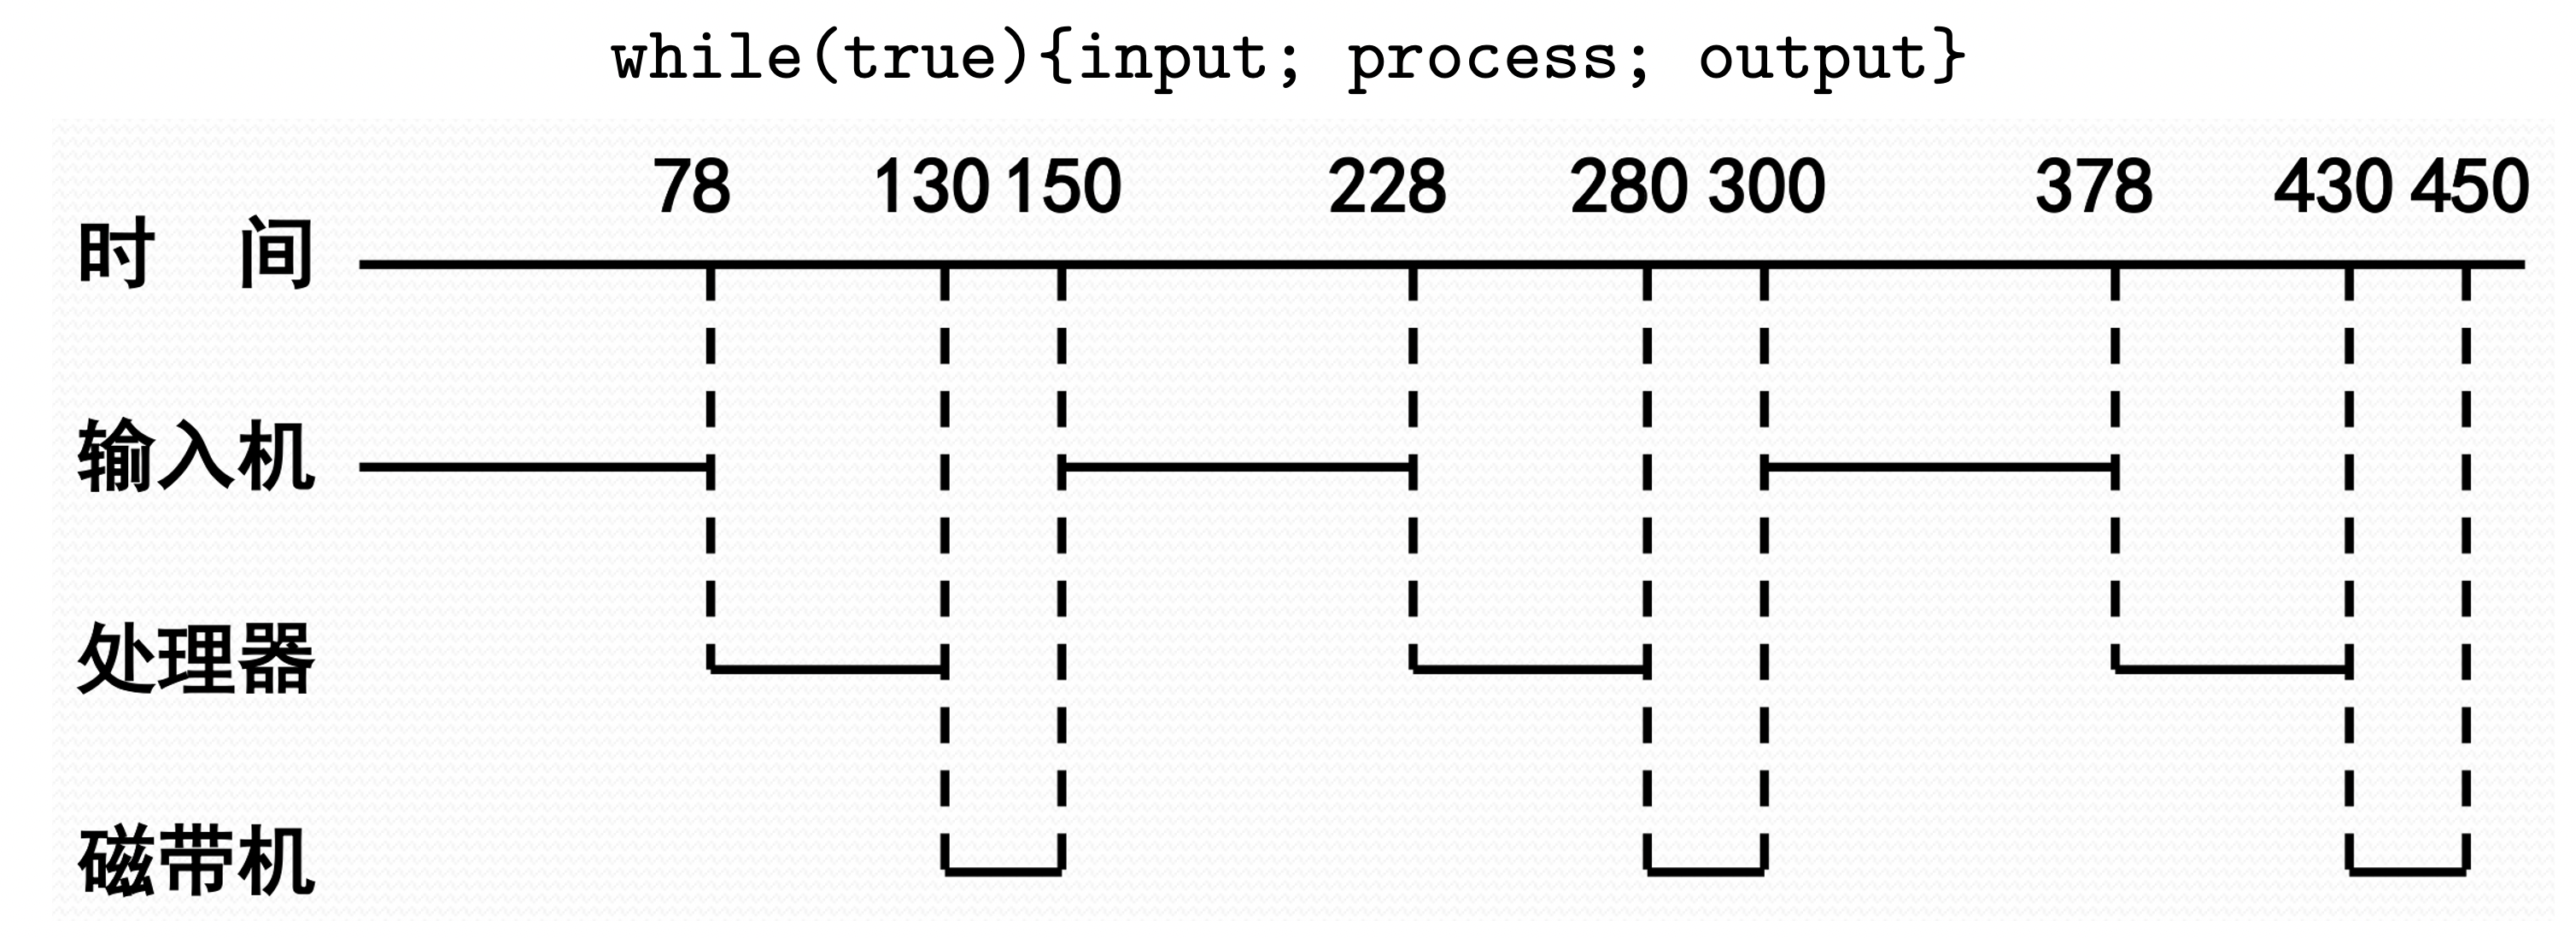
\includegraphics[width=0.65\textwidth]{img/6.1.1.2.1}
	\end{figure}

	换一种设计思路,设计3个独立运行的程序,让它们同时进入多道程序系统去并发执行
	\begin{itemize}
		\item 假定循环次数为$n$,处理器的使用效率$=(52n)/(78n+52+20)$,当$n \to \infty$时,处理器的使用效率约为67\%
	\end{itemize}

	\begin{figure}[H]
		\centering
		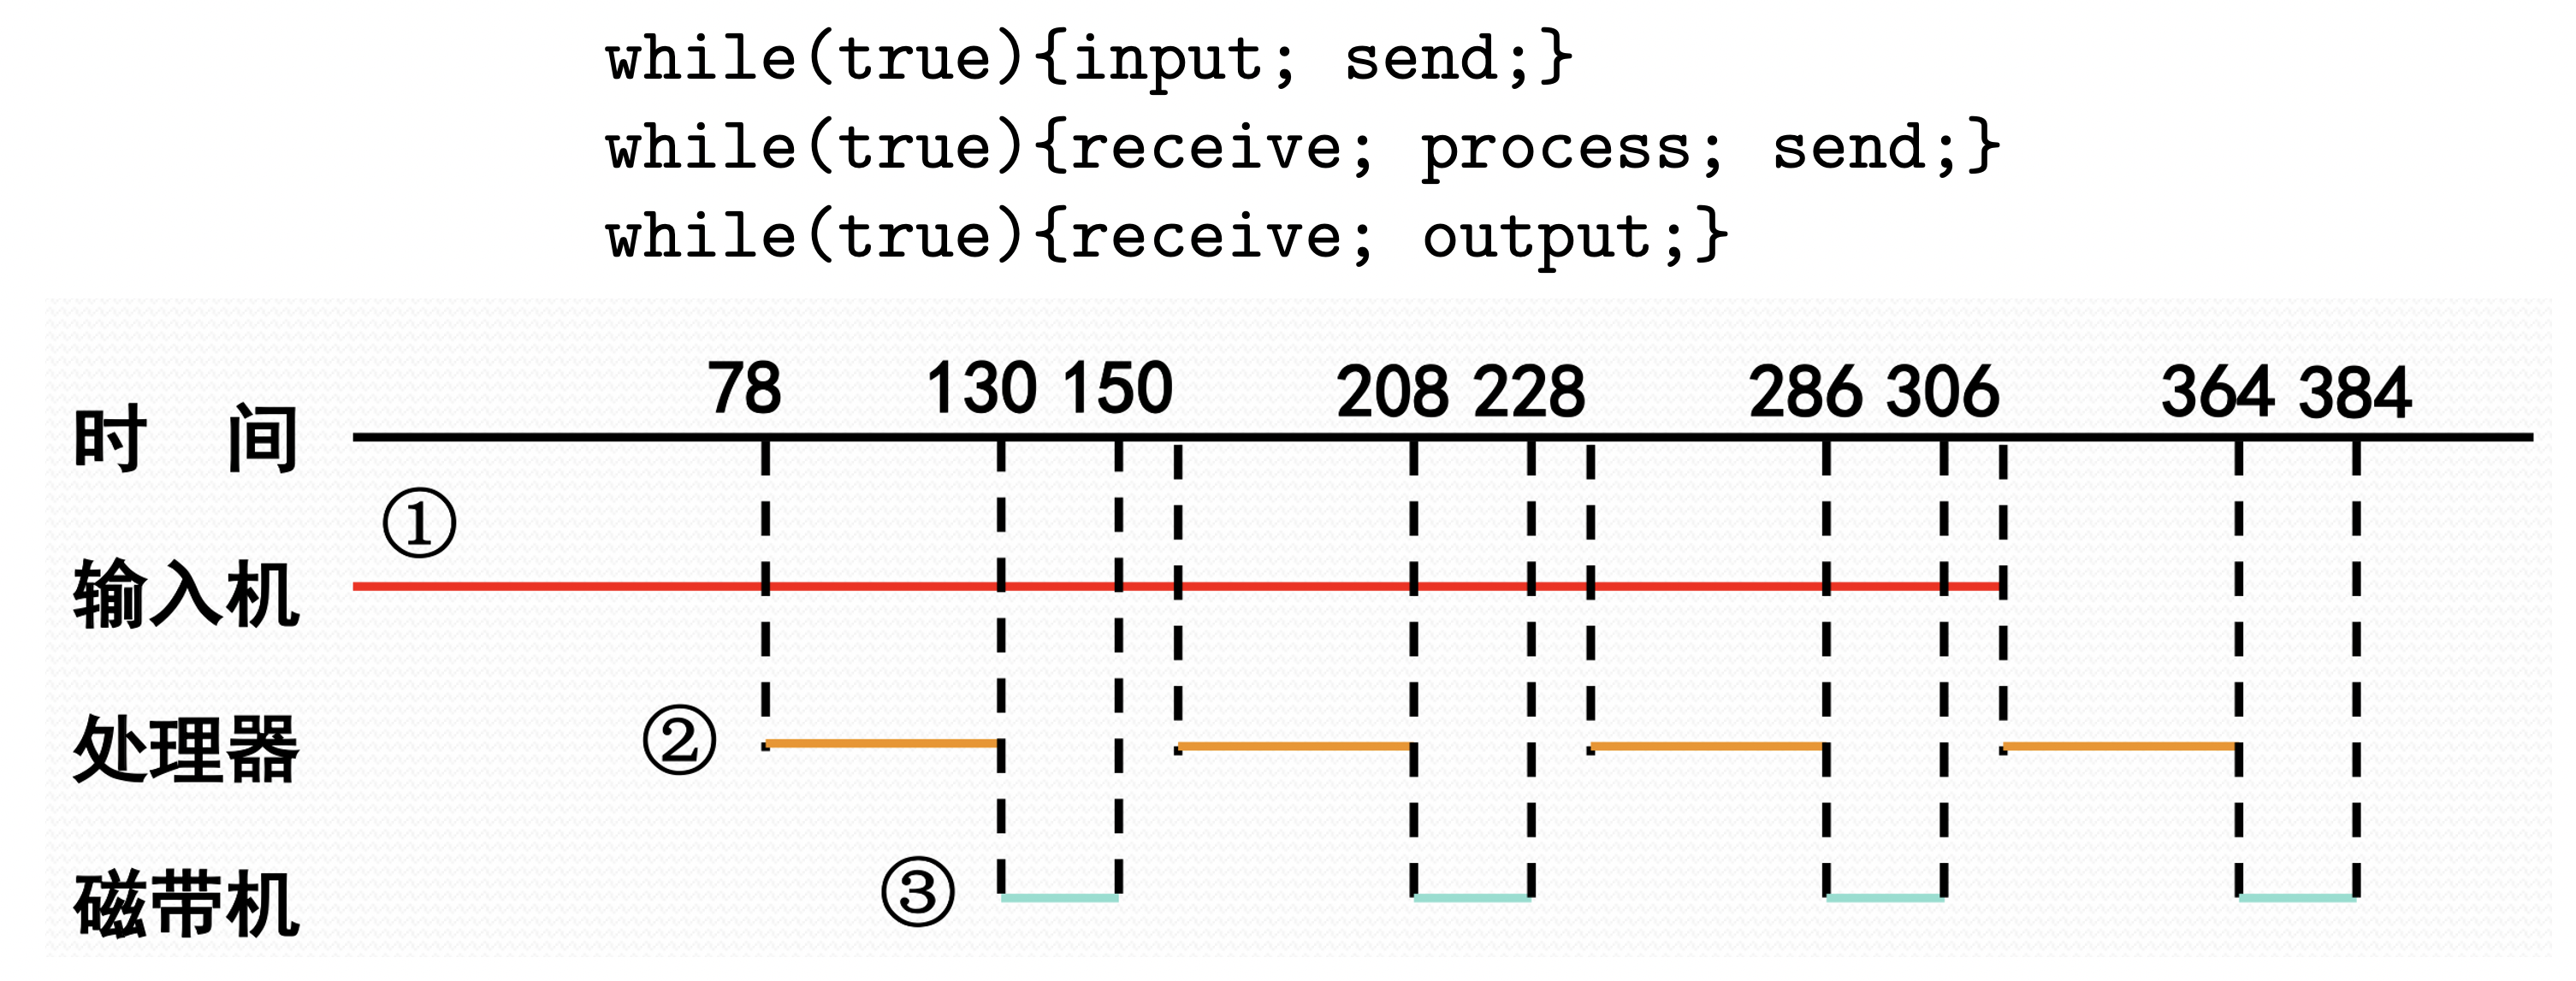
\includegraphics[width=0.65\textwidth]{img/6.1.1.2.2}
	\end{figure}

	顺序程序设计与并发程序设计
	\begin{figure}[H]
		\centering
		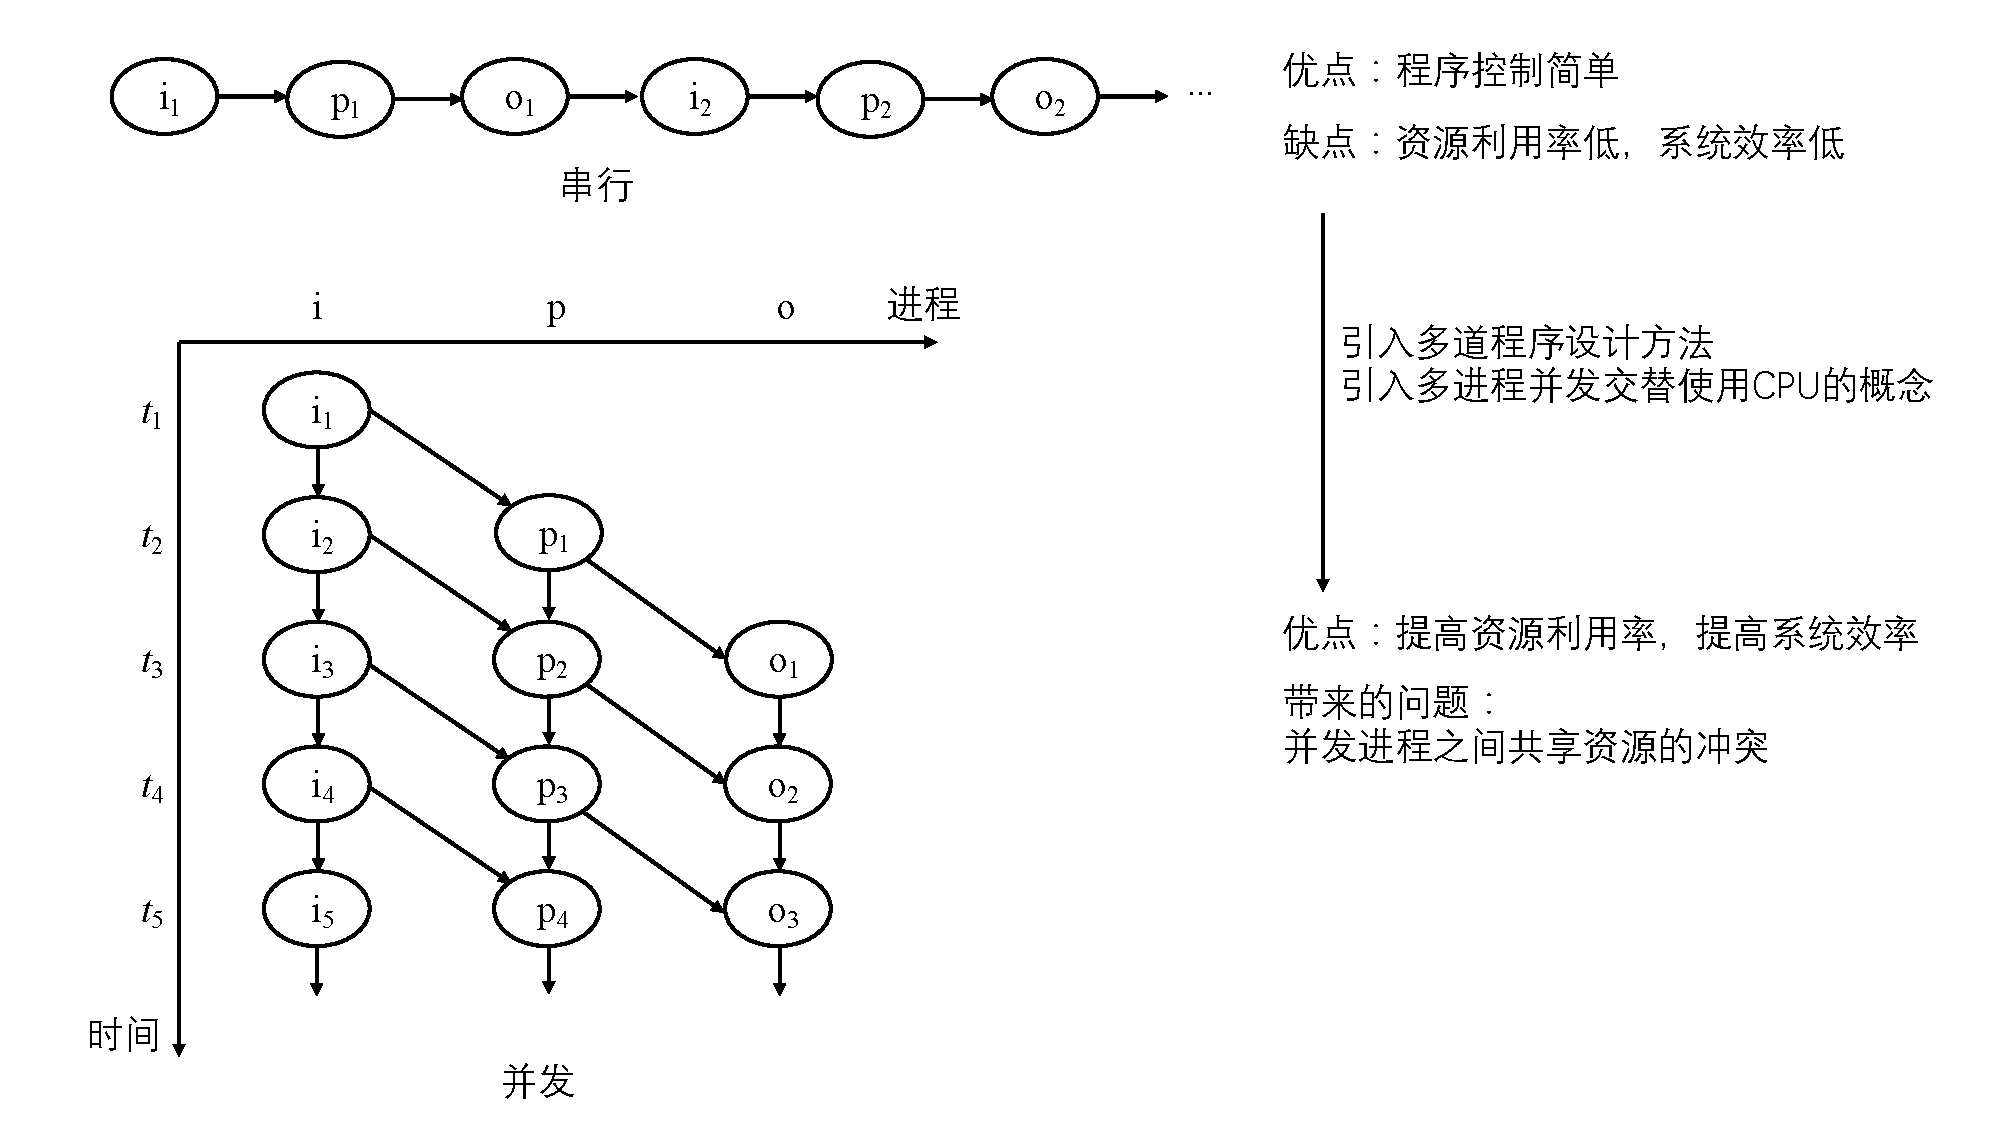
\includegraphics[width=0.75\textwidth]{img/6.1.1.2.3}
	\end{figure}

	程序并发执行是指一组程序的执行在\textbf{时间上是重叠}的,所谓重叠的是指一个程序执行第一条指令是在另一个程序执行完最后一条指令之前开始的
	\begin{itemize}
		\item 在宏观上,并发性反应了一个时间段内有几个程序都处于运行但运行尚未结束的状态
		\item 在微观上,任一时刻都只有一个程序在运行
		\item 并发实质上是处理器在几个程序之间的多路复用,对有限物力资源强制性使多用户共享,消除计算机部件之间的互等现象,提高资源利用率
		\item 并发使得程序失去了封闭性、顺序性、确定性和可再现性
	\end{itemize}

	并发程序设计的特性:
	\begin{itemize}
		\item \textbf{并行性:}多个进程在多道程序系统中并发执行或者在多处理器系统中并行执行,提高了计算效率
		\item \textbf{共享性:}多个进程共享软件资源
		\item \textbf{交互性:}多个进程并发执行时存在制约,增加了程序设计的难度
	\end{itemize}

	并发程序设计的优点:
	\begin{itemize}
		\item 对于单处理器系统,能够有效利用资源,让处理器和设备、设备和设备同时工作,充分发挥硬件设备的并行工作能力
		\item 对于多处理器系统,能够让进程在不同处理器上物理地并行工作,加快计算速度
		\item 对于简化程序设计而言,编写并发执行的小程序进度较快,更容易保证正确性
	\end{itemize}

	\subsection{并发进程的制约关系}

	\subsubsection{无关与交互的并发进程}
	并发进程可能是无关的,也可能是交互的
	\begin{itemize}
		\item 无关的并发进程:一组并发进程分别在不同的变量集合上运行,一个进程的执行与其他并发进程的进展无关
		\item 交往的并发进程:一组并发进程共享某些变量,一个进程的执行可能影响其他并发进程的结果
	\end{itemize}

	并发进程的无关性是进程的执行与时间无关的一个充分条件,该条件在1966年由Bernstein提出。假设:
	$$
	\begin{aligned}
		& R(P_i)={a_{1},a_{2},\cdots, a_{n}},\ \mbox{表示程序}P_i\mbox{在执行期间所引用的变量集} \\
		& W(P_i)={b_{1},b_{2},\cdots b_{m}},\ \mbox{表示程序}P_i\mbox{在执行期间所改变的变量集}
	\end{aligned}
	$$
	若两个进程的程序$P_1$和$P_2$能满足 Bernstein 条件,即引用变量集与改变变量集的交集为空集:
	$$R(P_1)\cap W(P_2) \cup R(P_2) \cap W(P_1) \cup W(P_1) \cap W(P_2) = \emptyset$$
	则并发进程的执行与时间无关,并发执行的程序可以保持封闭性和可再现性。
	\begin{itemize}
		\item $R(P_1)\cap W(P_2) \cup R(P_2) \cap W(P_1)$,表明一个程序在两次读操作之间存储单元的数据不会被改变
		\item $W(P_1) \cap W(P_2)$,表明程序的写操作结果不会丢失
	\end{itemize}

	\textbf{例:}有如下四条语句
	$$S_1:a=x+y; \ S_2:b=z+1;\ S_3:c=a-b;\ S_4:w=c+1$$
	于是有:$R(S_1)=\{x,y\},\ R(S_2)=\{z\},\ R(S_3)=\{a,b\},\ R(S_4)=\{c\};\ W(S_1)=\{a\},\ W(S_2)=\{b\},\ W(S_3)=\{c\},\ W(S_4)=\{w\}$
	\begin{itemize}
		\item 因为$S_1$和$S_2$满足 Bernstein 条件,所以它们可以并发执行
		\item 而其他语句之间因变量交集之并不为空,表明它们之间是存在交互的,并发执行可能会产生与时间有关的错误
	\end{itemize}

	\subsubsection{与时间相关的程序设计错误}
	两个交互的并发进程,其中一个进程对另一个进程的影响往往是不可预期的,甚至是无法再现的
	\begin{itemize}
		\item 这是因为它们执行时的相对速度不可预测
	\end{itemize}
	
	由于一个进程的执行速度通常无法为另一个进程所预知,对于共享公共变量(资源)的并发进程而言,计算结果往往取决于这一组并发进程执行的相对速度,继而可能导致出现错误,这种错误称为与时间有关的错误
	\begin{itemize}
		\item 表现一:结果错误
		\item 表现二:永远等待
	\end{itemize}

	\paragraph{结果错误}~{}


	\begin{figure}[H]
		\centering
		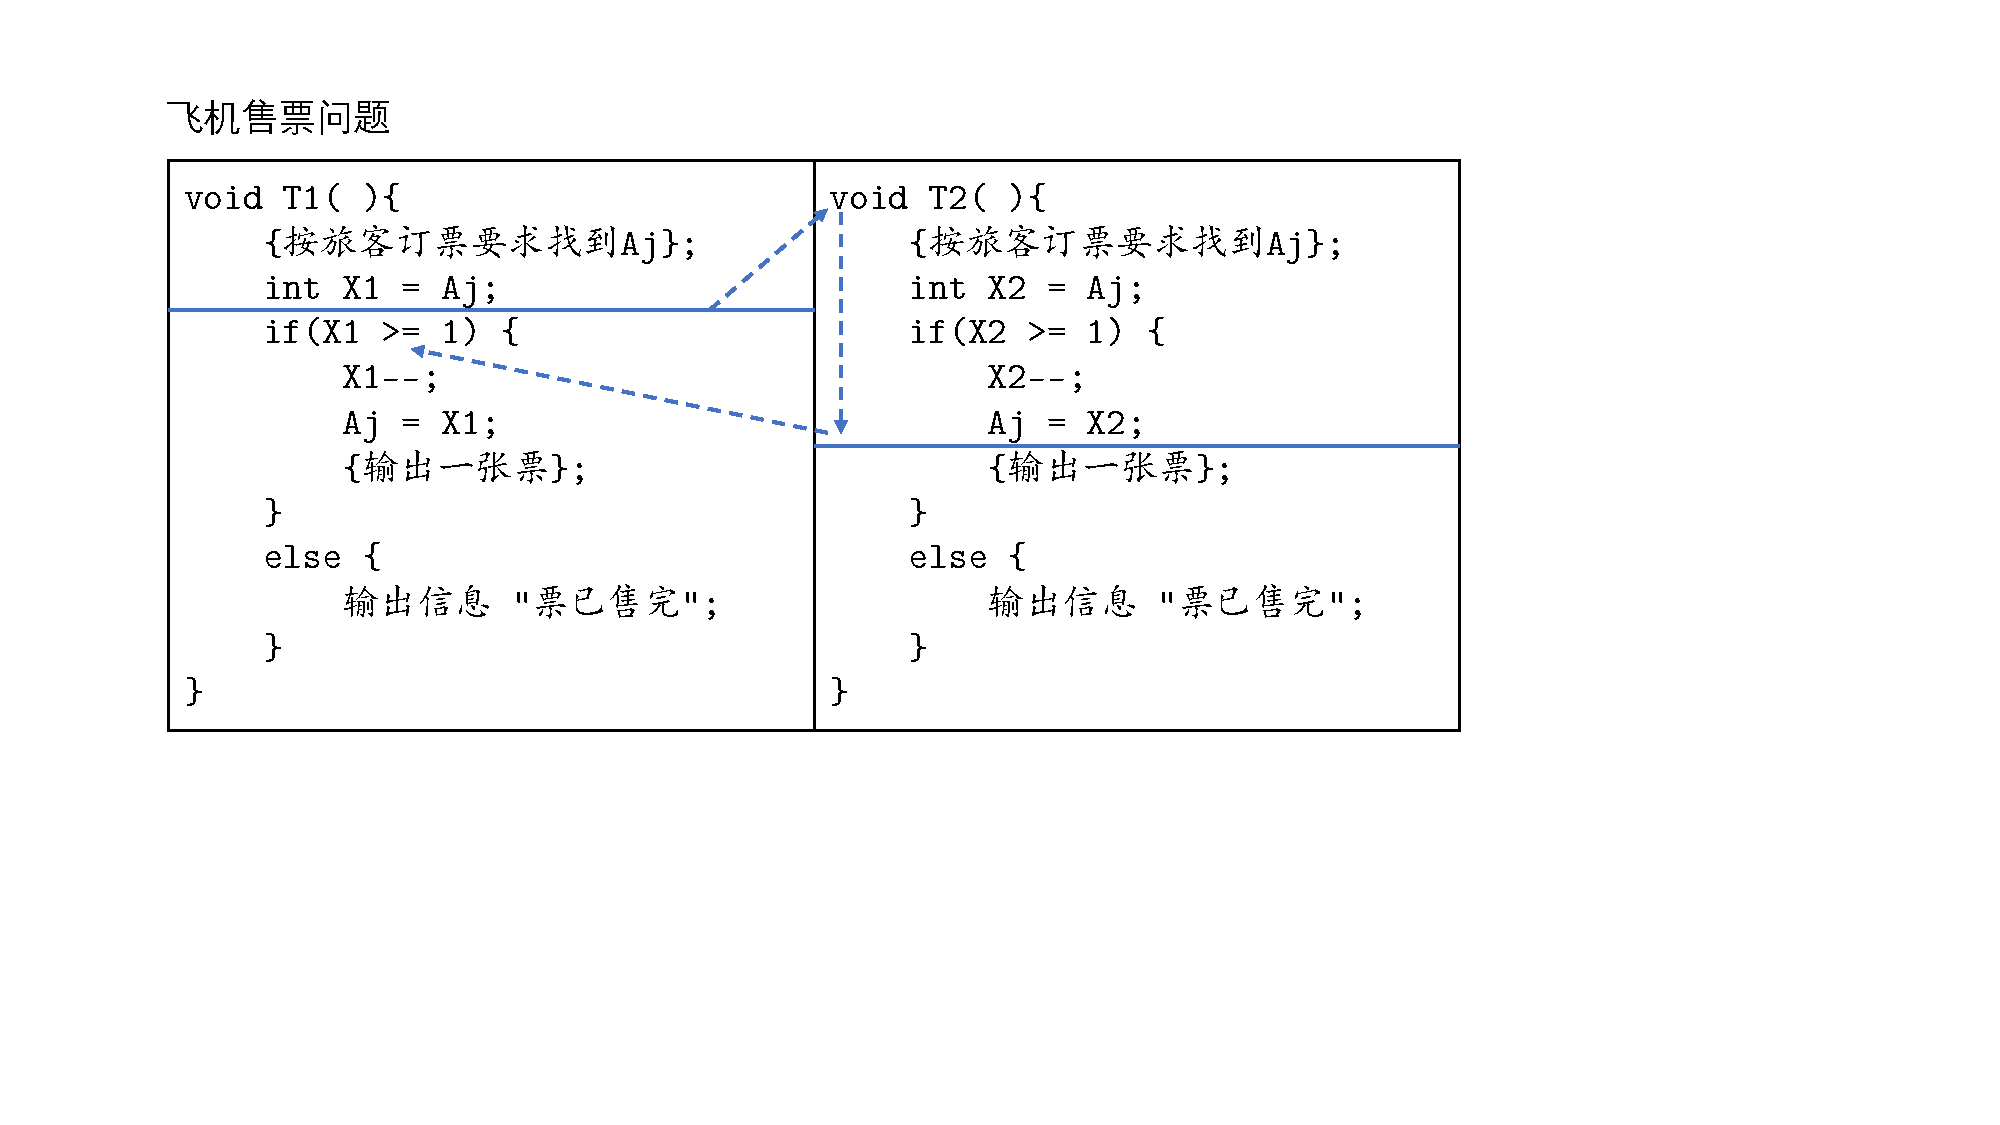
\includegraphics[width=0.75\textwidth]{img/飞机售票问题.pdf}
	\end{figure}

	可能出现如下调度情况
	\begin{lstlisting}[language=C,keywordstyle=\color{black}]
T1: X1 = A[j];                       /* X1 = m(m>0) */
T2: X2 = A[j];                       /* X2 = m */
T2: X2--; A[j] = X2; {输出一张票};   /* A[j] = m - 1 */
T1: X1--; A[j] = X1; {输出一张票};   /* A[j] = m - 1 */
	\end{lstlisting}

	此时出现把同一张票卖给两个旅客的情况
	\begin{itemize}
		\item 两个旅客可能各自都买到一张同天同次航班的机票,可是\verb|A[j]|的值实际上只减去1,造成余票数不正确
		\item 特别是,当某次航班只有一张余票时,可能把一张票同时售给两位旅客
	\end{itemize}


	\paragraph{永远等待}~{}

	\begin{figure}[H]
		\centering
		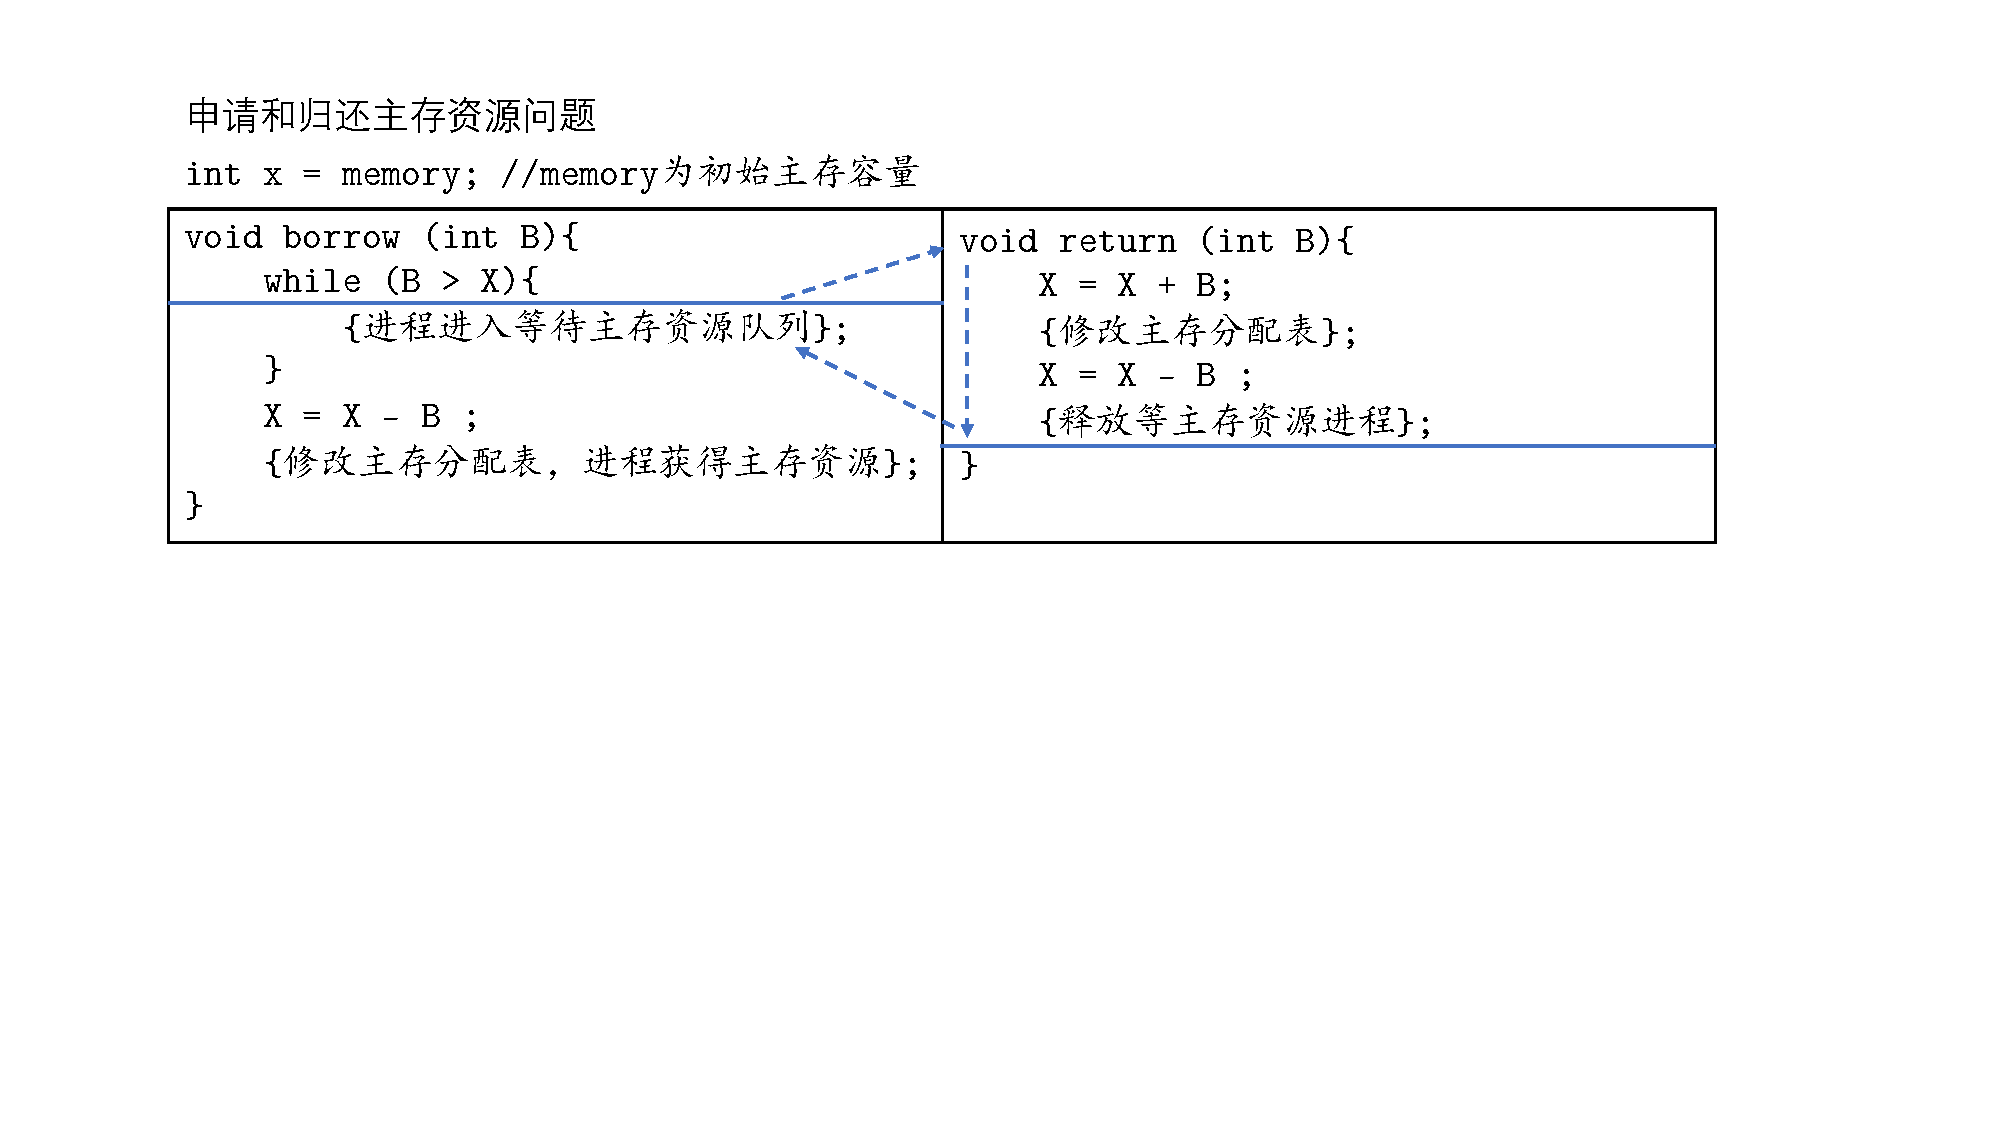
\includegraphics[width=0.85\textwidth]{img/申请和归还主存资源问题.pdf}
	\end{figure}

	由于borrow和return共享代表主存物理资源的临界变量X,对并发执行不加限制会导致错误。例如:
	\begin{itemize}
		\item 进程P调用borrow()申请主存资源,在执行比较B和X的大小的指令后,发现B>X条件成立,但在执行{进程进入等待主存资源队列}之前被抢占
		\item 进程Q调用return()抢先执行,归还所借全部主存资源
		\item 这时,由于进程P尚未成为等待者,return()中的{释放等待主存资源进程}相当于空操作,当调用borrow()的应用进程再次获得处理器时,因此前判断B>X条件成立,将正式进入等待主存资源队列,假设后续没有其他进程再来归还主存资源,那么,已经进入等待主存资源队列的进程将处于永远等待的状态
	\end{itemize}
	
	
	\subsubsection{进程执行的制约关系}

	交互的并发进程在执行时的制约关系包括两类:进程互斥与进程同步。只有有效解决进程互斥与进程同步这两种制约关系,才能保证并发进程在交互的执行过程中能够得到合理的结果。

	\begin{figure}[H]
		\centering
		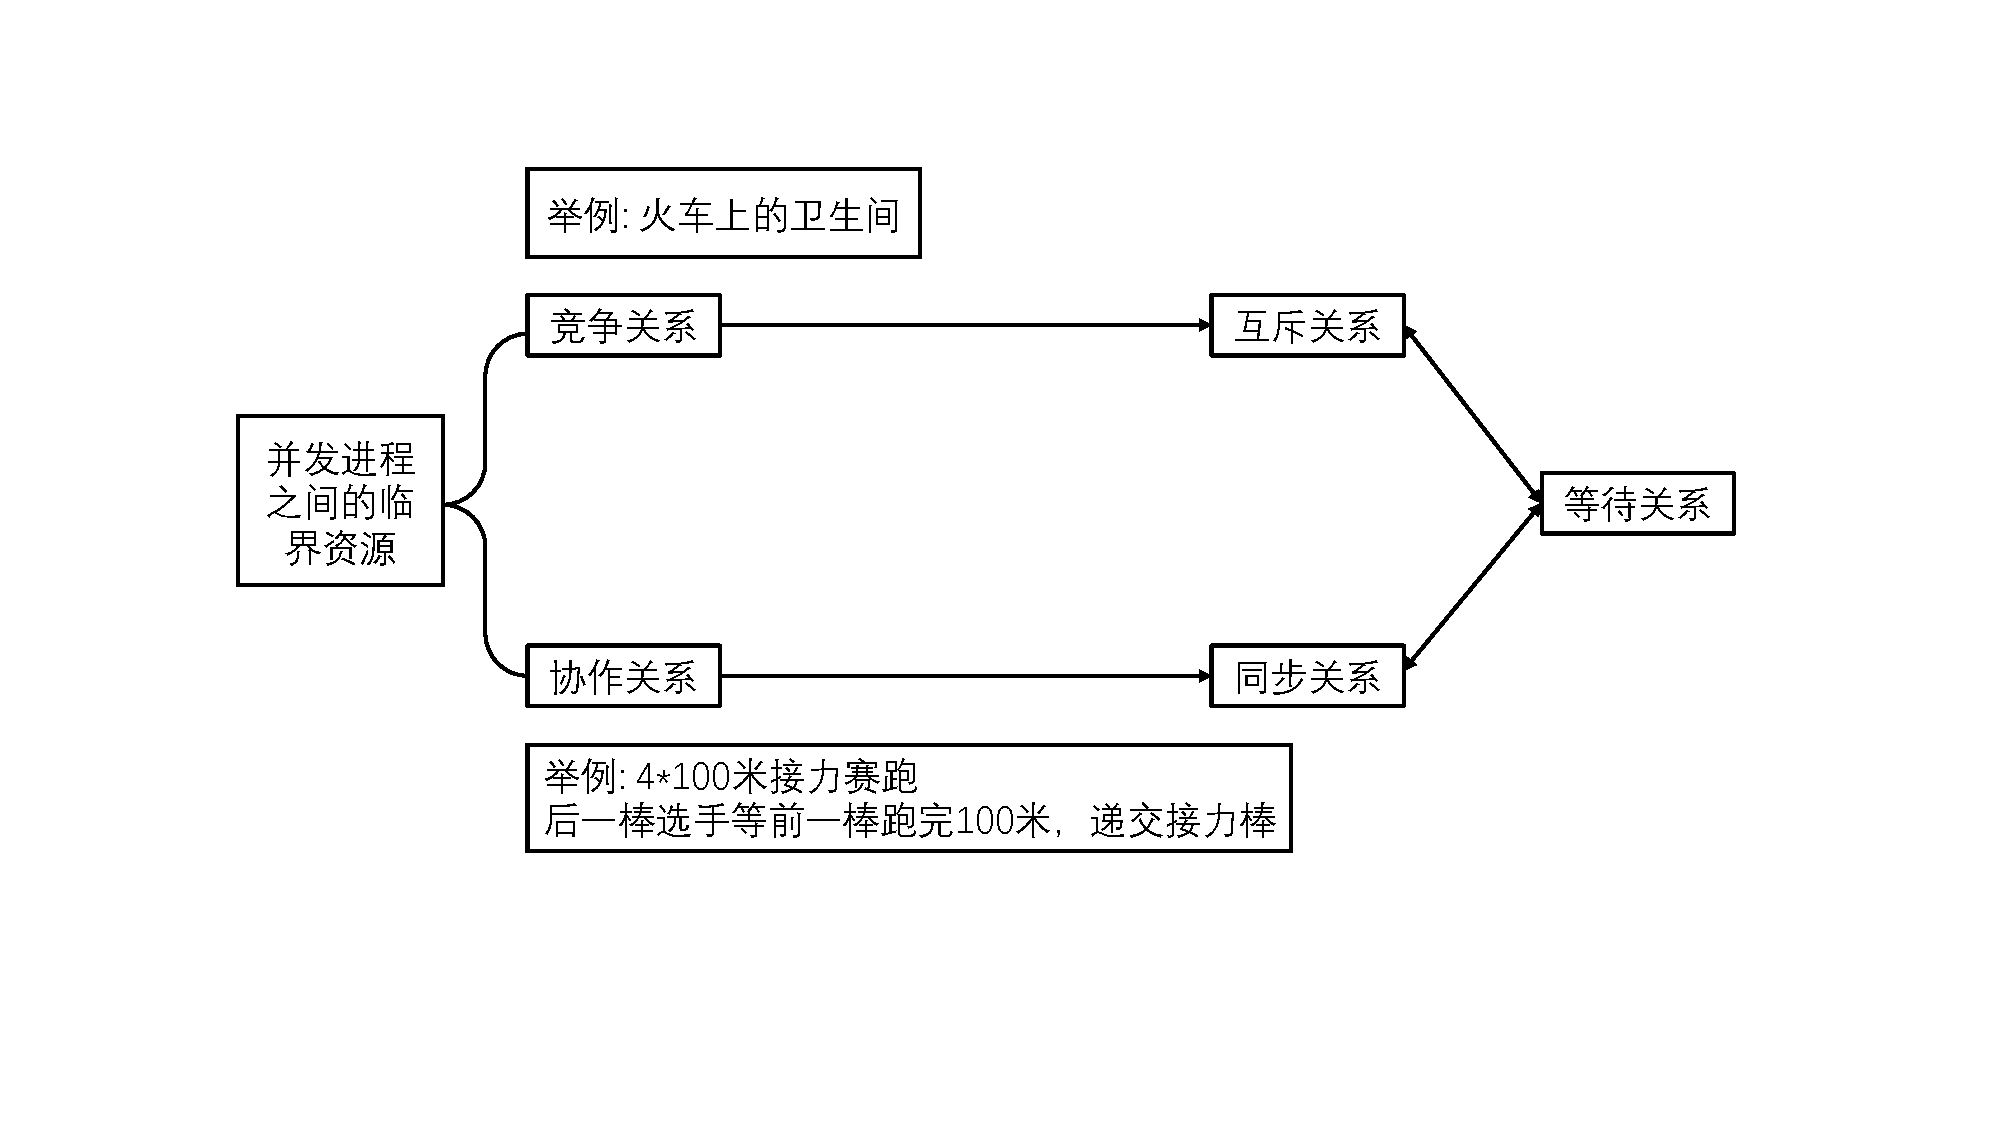
\includegraphics[width=0.65\textwidth]{img/6.1.2.3}
	\end{figure}

	\paragraph{进程互斥(竞争)}~{}

	进程互斥是指并发进程之间因相互争夺独占性资源而产生的竞争制约关系
	\begin{itemize}
		\item 一个进程的执行可能影响到同其竞争资源的其他进程,如果两个进程要访问同一资源,那么,一个进程通过操作系统分配得到该资源,另一个将不得不等待
		\item 资源竞争带来的的两个控制问题:
		\begin{itemize}
			\item 一个是死锁问题:一组进程如果都获得了部分资源,还想要得到其他进程所占有的资源,最终所有的进程将陷入死锁
			\begin{figure}[H]
				\centering
				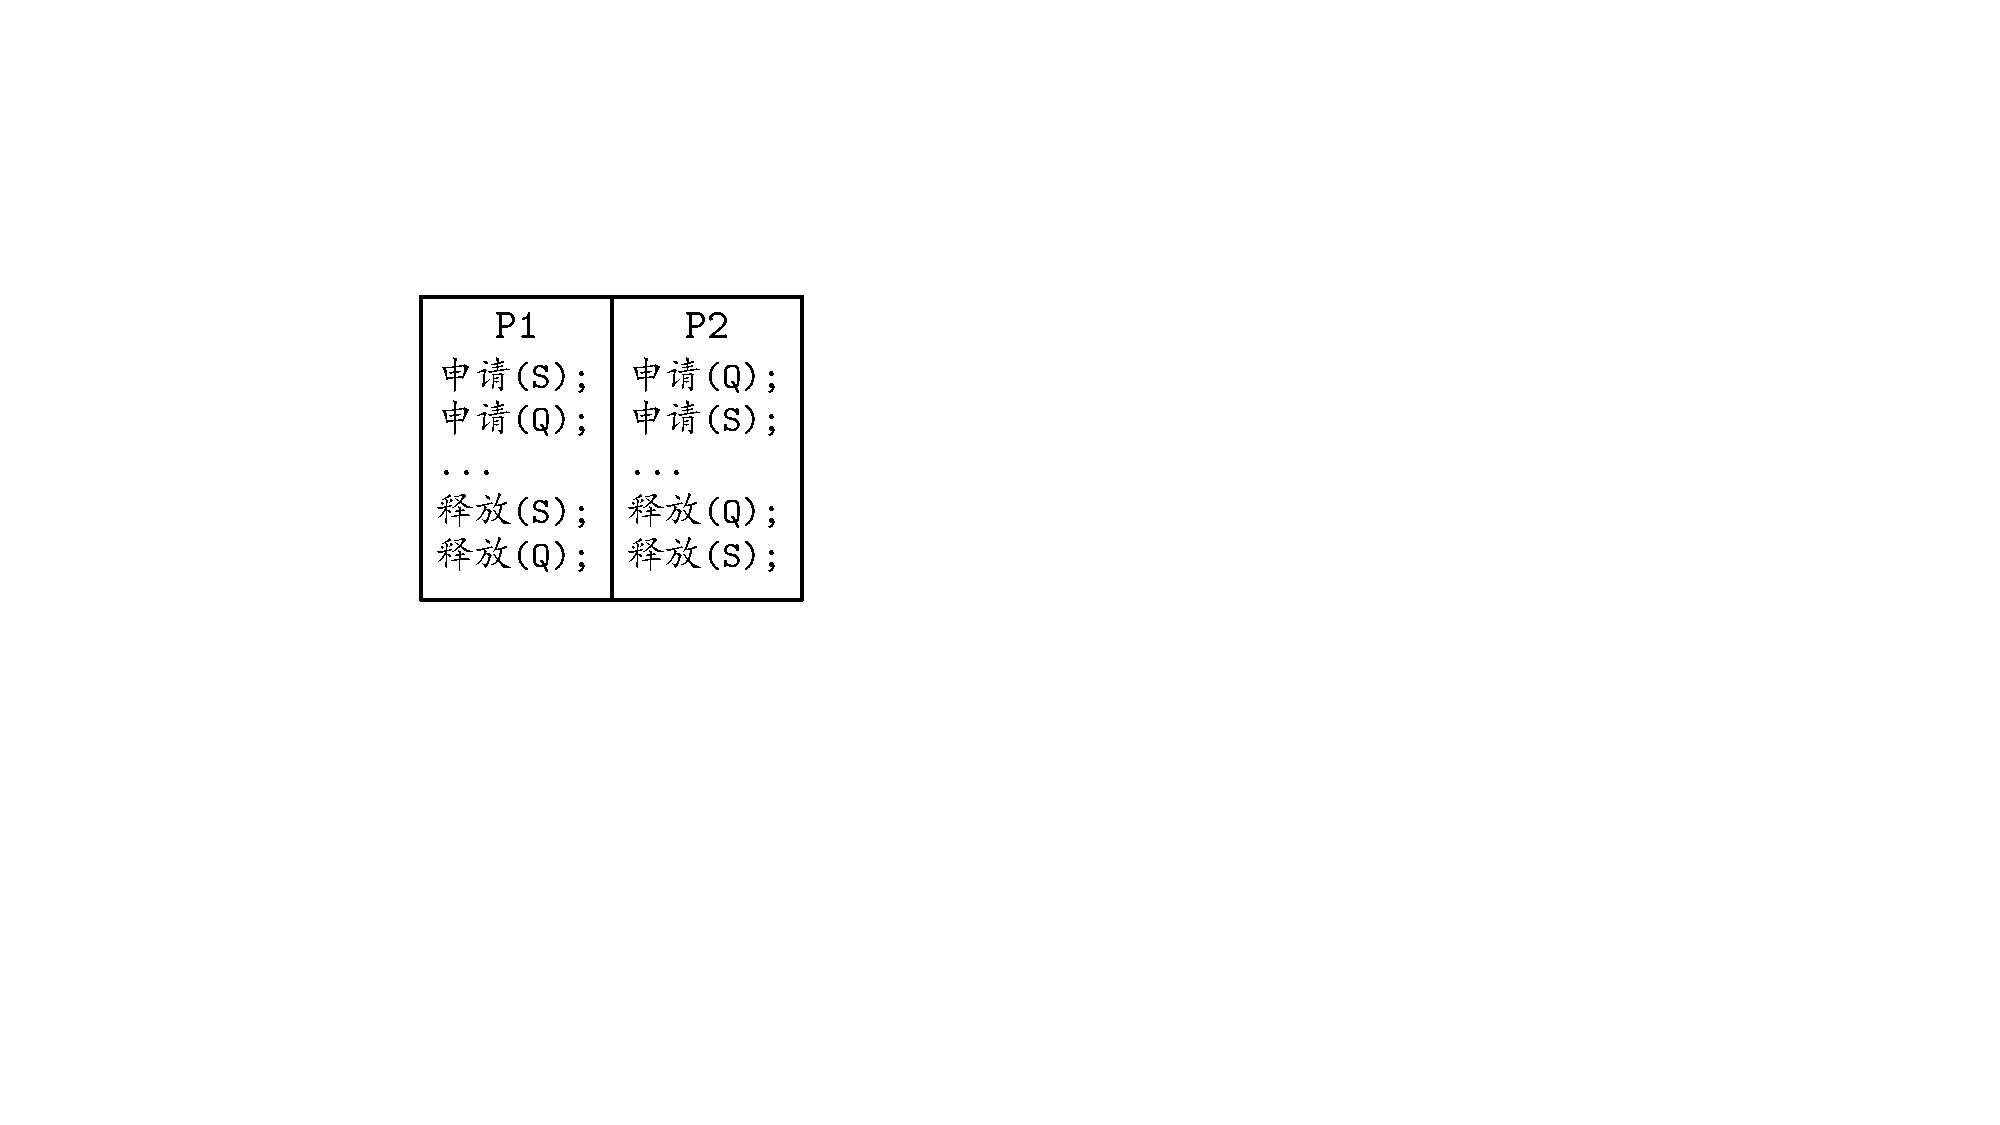
\includegraphics[width=0.2\textwidth]{img/6.1.2.3.1}
			\end{figure}
			\item 一个是饥饿问题:一个进程由于其他进程总是优先于它而被无限期拖延
			\item 操作系统需要保证诸进程能互斥地访问临界资源,既要解决饥饿问题,又要解决死锁问题
		\end{itemize}
	\end{itemize}

	\paragraph{进程同步(协作)}~{}

	进程同步是指并发进程之间为完成共同任务基于某个条件来协调执行先后关系而产生的协作制约关系
	\begin{itemize}
		\item 两个及以上进程基于某个条件来协调它们的活动。一个进程的执行依赖于另一个协作进程的消息或信号,当一个进程没有得到来自于另一个进程的消息或信号时则需等待,直到消息或信号到达才被唤醒
		\item 进程互斥关系是一种特殊的进程同步关系,即逐次使用互斥共享资源,是对进程使用资源次序上的一种协调
	\end{itemize}

	\subsection{操作系统并发问题解决方案}
	\begin{table}[H]
	\centering
	\resizebox{\textwidth}{!}{
	\begin{tabular}{|c|c|c|c|c|}
	\hline
	原语类型                    & 采用策略                                                                & 同步机制                                                                           & 适用场合                                                                                 & 方向                                                                                        \\ \hline
	高级通信原语                  & \begin{tabular}[c]{@{}c@{}}采用消息传递、共享\\ 内存、共享文件策略\end{tabular}       & \begin{tabular}[c]{@{}c@{}}消息队列、共享\\ 内存、管道通信\end{tabular}                      & \begin{tabular}[c]{@{}c@{}}解决并发进程通信、同步和\\ 互斥问题,适用于面向语句\\ 的高级程序设计\end{tabular}        & \multirow{4}{*}{\begin{tabular}[c]{@{}c@{}}上\\ ↑\\ 自\\ 底\\ 向\\ 上\\ ↓\\ 底\end{tabular}} \\ \cline{1-4}
	\multirow{3}{*}{低级通信原语} & \begin{tabular}[c]{@{}c@{}}采用阻塞/唤醒+集\\ 中临界区(1次测试)\\ 策略\end{tabular} & 管程                                                                             & \begin{tabular}[c]{@{}c@{}}解决并发进程同步和互斥\\ 问题,不能传递消息,适\\ 用于面向语句的高级程序\\ 设计\end{tabular} &                                                                                           \\ \cline{2-4}
							& \begin{tabular}[c]{@{}c@{}}采用阻塞/唤醒+分散\\ 临界区(1次测试)\\ 策略\end{tabular} & 信号量和PV操作                                                                       & \begin{tabular}[c]{@{}c@{}}解决并发进程同步和互斥\\ 问题,不能传递消息,适\\ 用于面向指令的低级程序\\ 设计\end{tabular} &                                                                                           \\ \cline{2-4}
							& \begin{tabular}[c]{@{}c@{}}采用忙式等待(反\\ 复测试)策略\end{tabular}           & \begin{tabular}[c]{@{}c@{}}关中断、对换、测\\ 试并建立、peterson\\ 算法、dekker算法\end{tabular} & \begin{tabular}[c]{@{}c@{}}解决并发进程互斥问题,\\ 不能传递消息,适用于面\\ 向指令的低级程序设计\end{tabular}       &                                                                                           \\ \hline
	\end{tabular}
	}
	\end{table}

	\section{临界区管理}

	\subsection{临界区的概念}
	并发进程中与共享变量有关的程序段叫“\textbf{临界区}”,共享变量代表的资源叫“\textbf{临界资源}”
	\begin{itemize}
		\item 与同一变量有关的临界区分散在各进程的程序段中,而各进程的执行速度不可预见
		\item 如果保证进程在临界区执行时,不让另一个进程进入临界区,即各进程对共享变量的访问是互斥的,就不会造成与时间有关的错误
	\end{itemize}

	关于临界区的概念是由Drikstra在1965年首先提出的。临界区在程序设计中的形式化定义如下,用\, \verb|shared|\, 表示共享变量
	\begin{lstlisting}[keywordstyle=\color{black}]
shared <varialbe>
region <varialbe> do <statement_list>
	\end{lstlisting}
	为了正确而有效地使用临界资源,共享变量的并发进程应遵守临界区调度的三个原则
	\begin{enumerate}[label=\arabic*.]
		\item 一次至多一个进程能够进入临界区内执行
		\item 如果已有进程在临界区,其他试图进入的进程应等待
		\item 进入临界区内的进程应在有限时间内退出,以便让等待进程中的一个进入
	\end{enumerate}

	\begin{figure}[H]
		\centering
		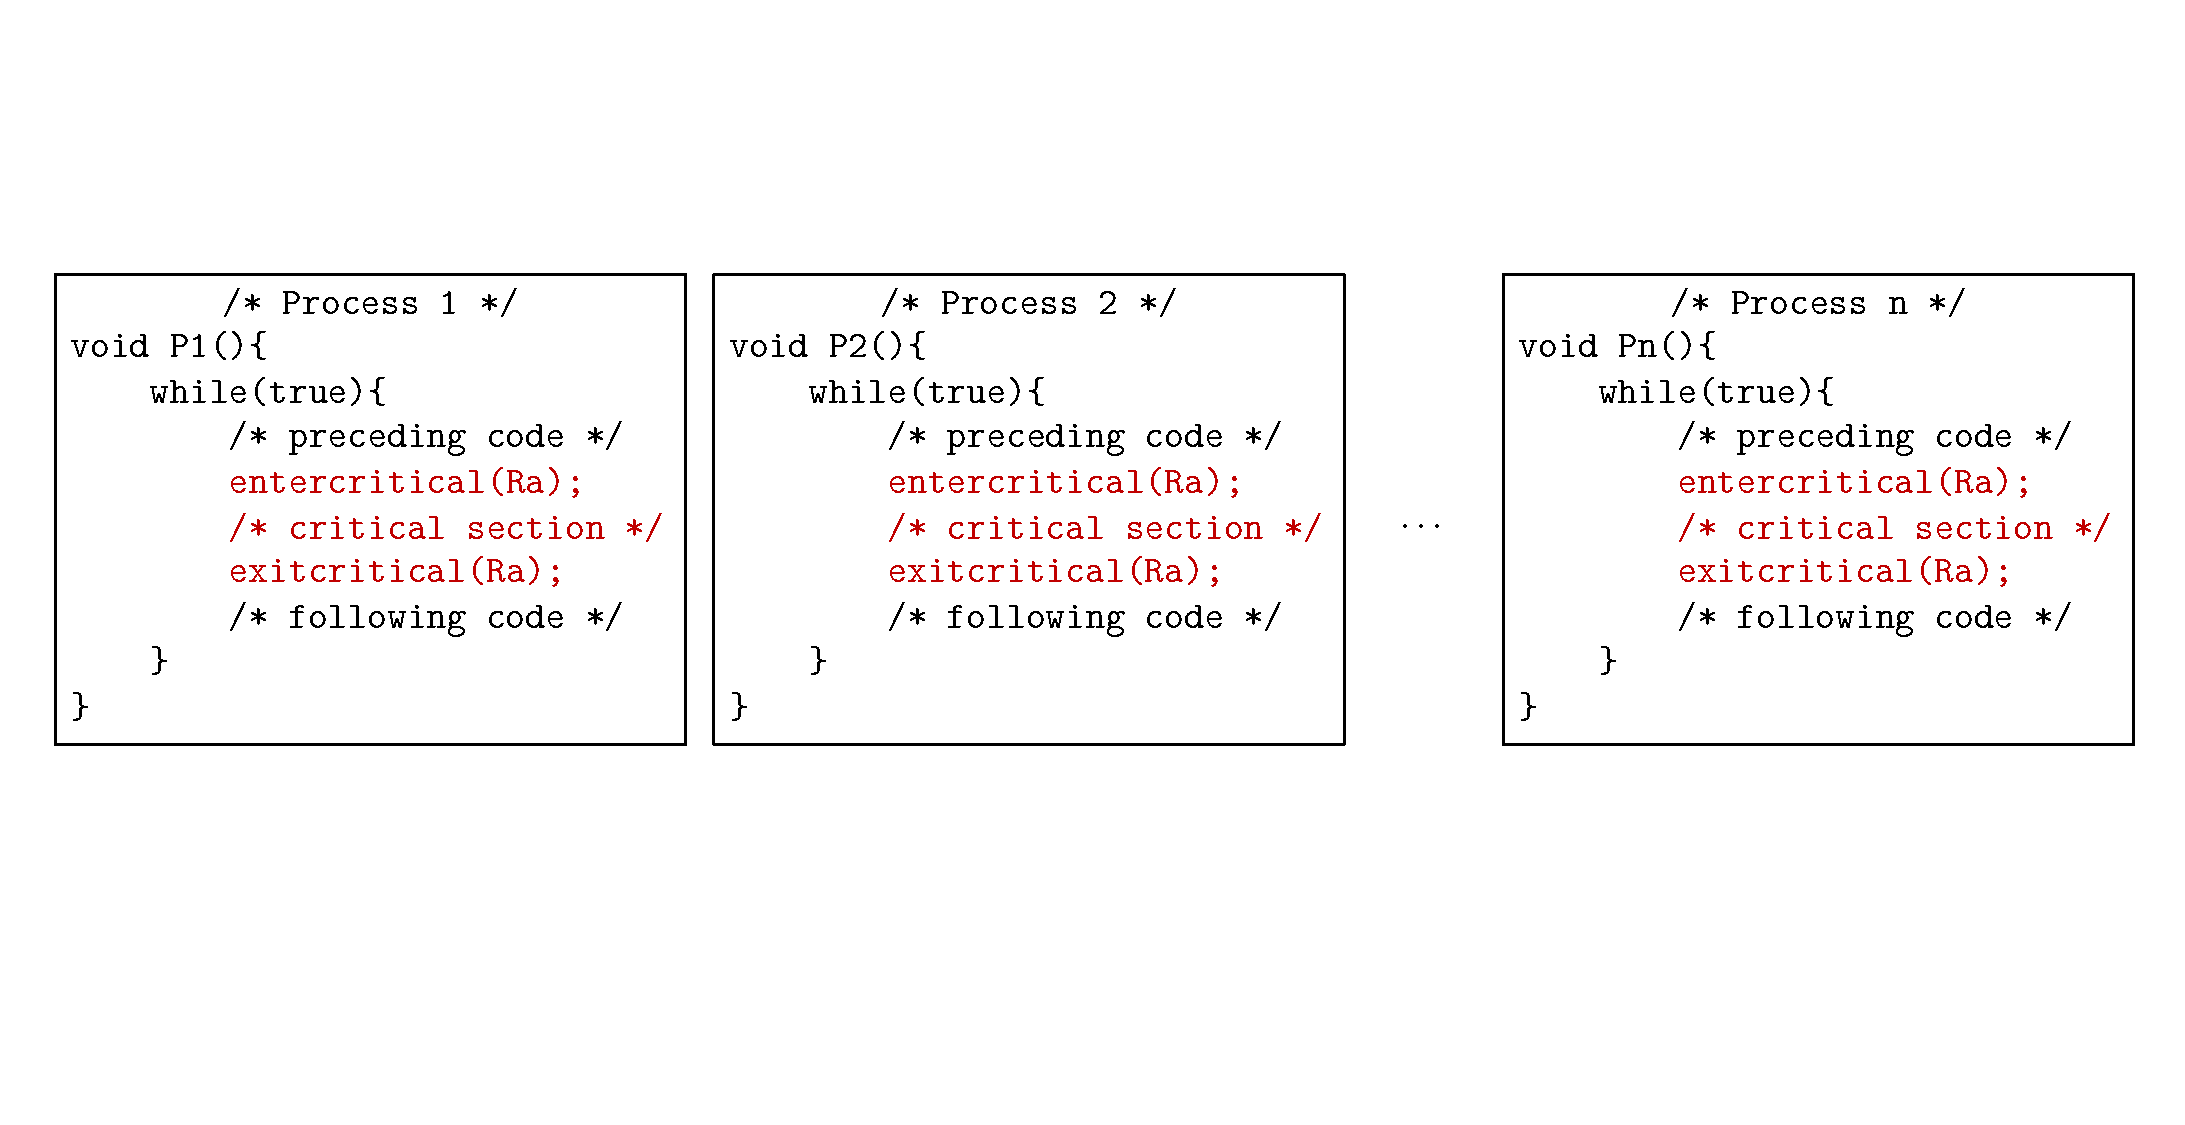
\includegraphics[width=0.98\textwidth]{img/互斥与临界区.pdf}
	\end{figure}

	临界区是允许嵌套的,其代码结构如下图(a)所示
	\begin{itemize}
		\item 但是随意或者不严谨的嵌套可能导致进程永久地留在其临界区内
		\item 如果另有一个进程执行,其代码如图(b)所示,这样,当两个进程在差不多的时间进入外层的临界区后,将发现每个进程都被排斥在内层临界区之外,造成无限地等待进入内层临界区,即临界区嵌套使用不当会产生死锁
	\end{itemize}

	\begin{figure}[H]
		\centering
		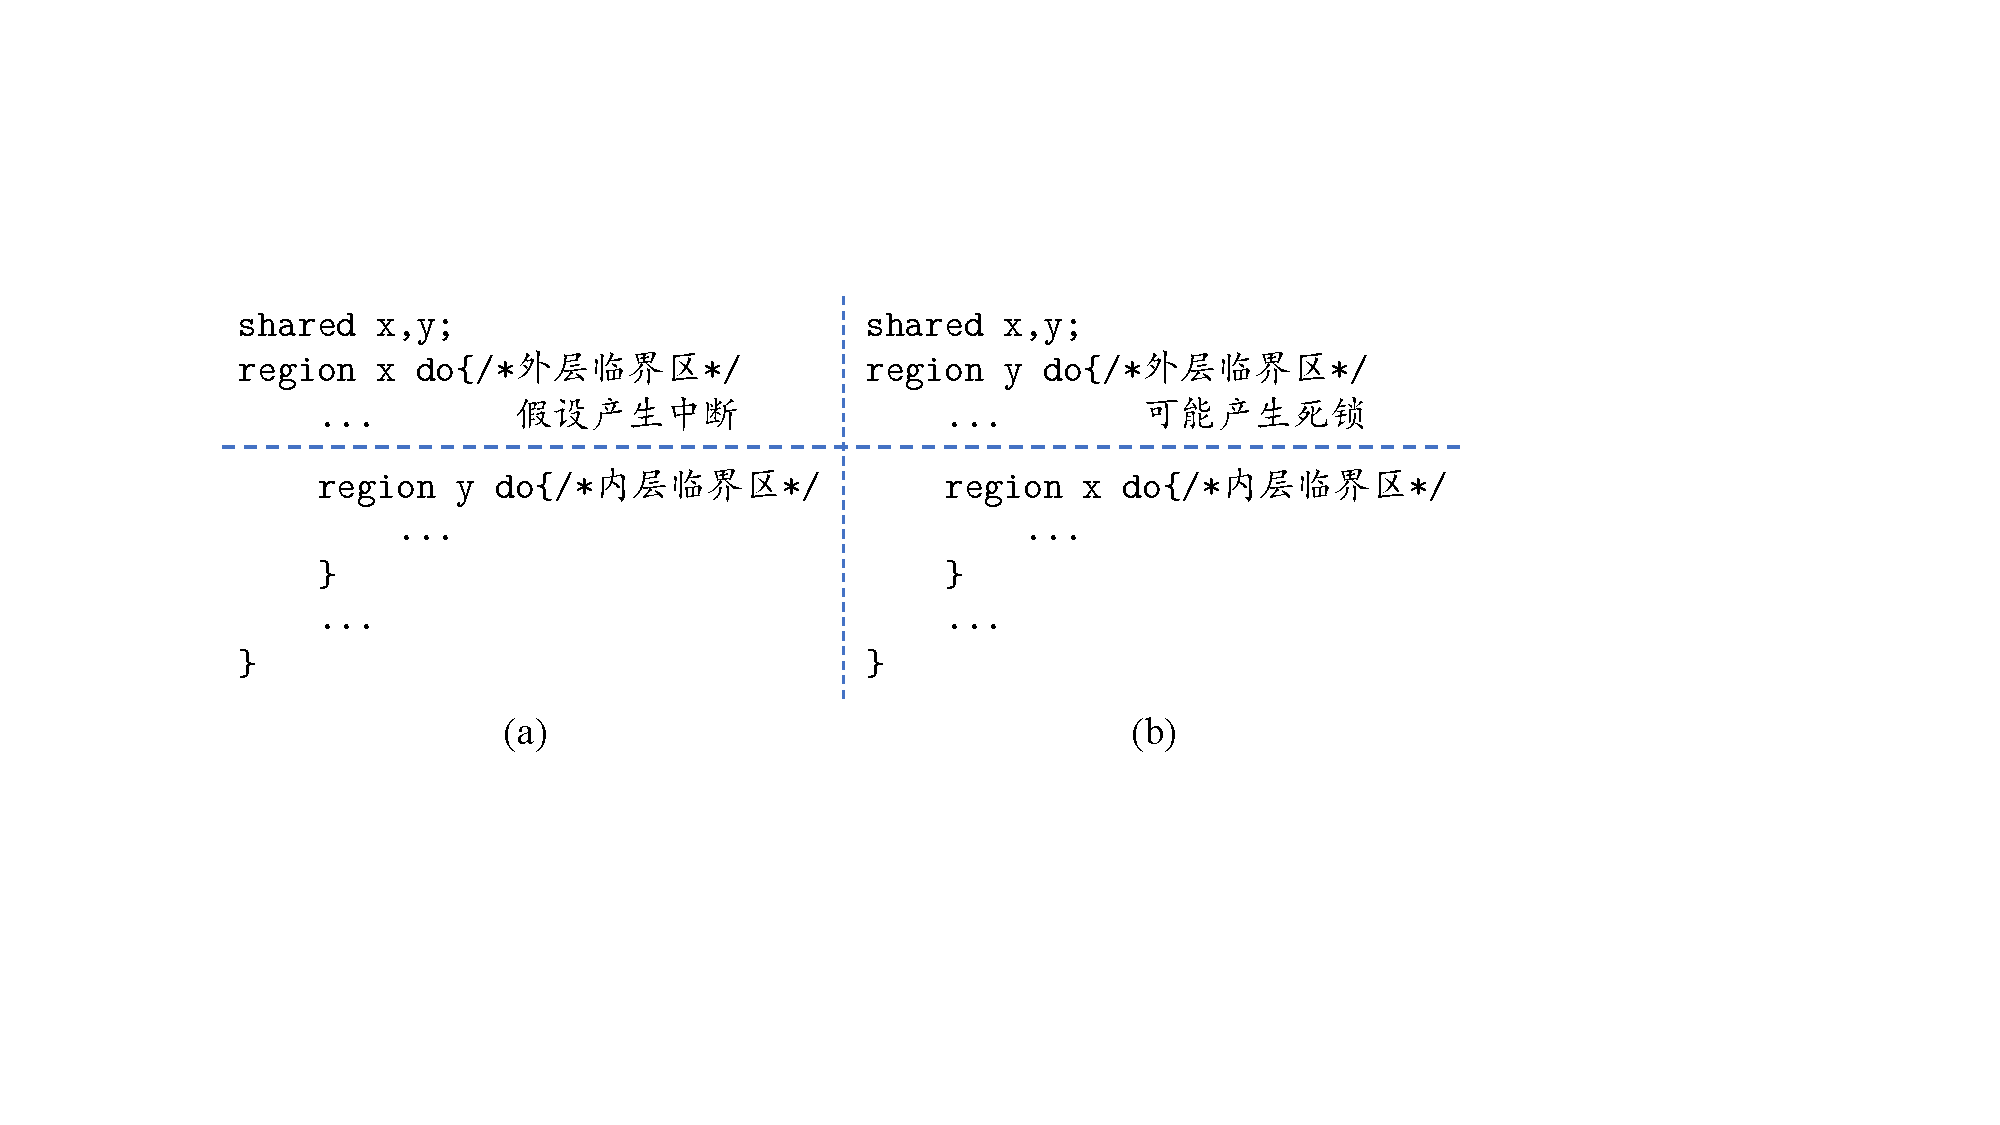
\includegraphics[width=0.7\textwidth]{img/临界区嵌套使用.pdf}
	\end{figure}


	\subsection{临界区管理实现的尝试}
	
	考虑并发进程在单处理器或共享内存的多处理器计算机系统上的执行情况,这里先讨论采用软件方法实现临界区管理
	\begin{itemize}
		\item 通常假设系统具有存储器访问级的基本互斥性,即同时访问内存中的同一个单元时,必定由存储器进行仲裁使其串行化
		\item 此外,硬件、操作系统或语言未提供任何支持
	\end{itemize}

	临界区管理可采用标志方式,即用标志来表示哪个进程可进入临界区
	
	第一种尝试如下:
	\begin{figure}[H]
		\centering
		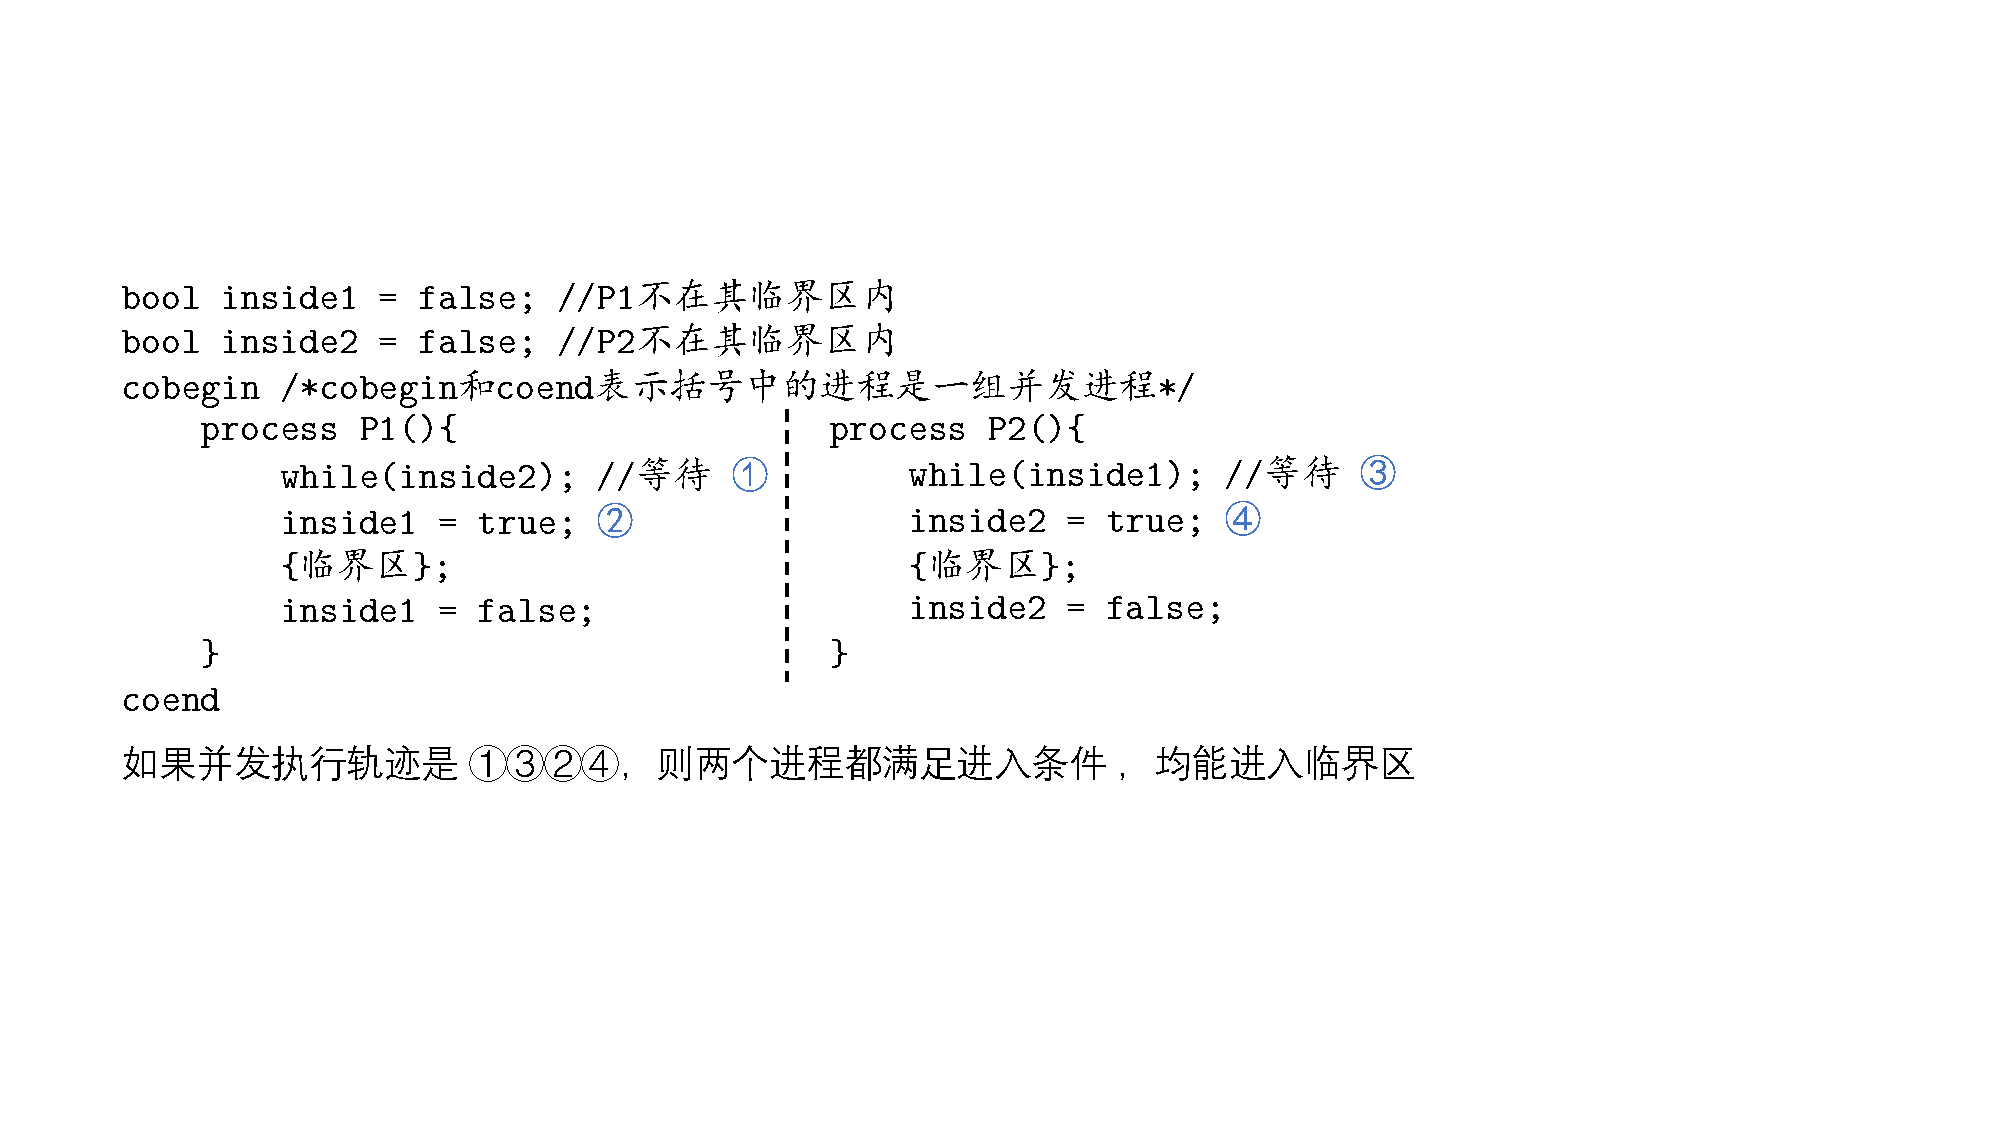
\includegraphics[width=0.8\textwidth]{img/临界区管理尝试1.pdf}
	\end{figure}

	第二种尝试是对第一种方案做修正:
	\begin{figure}[H]
		\centering
		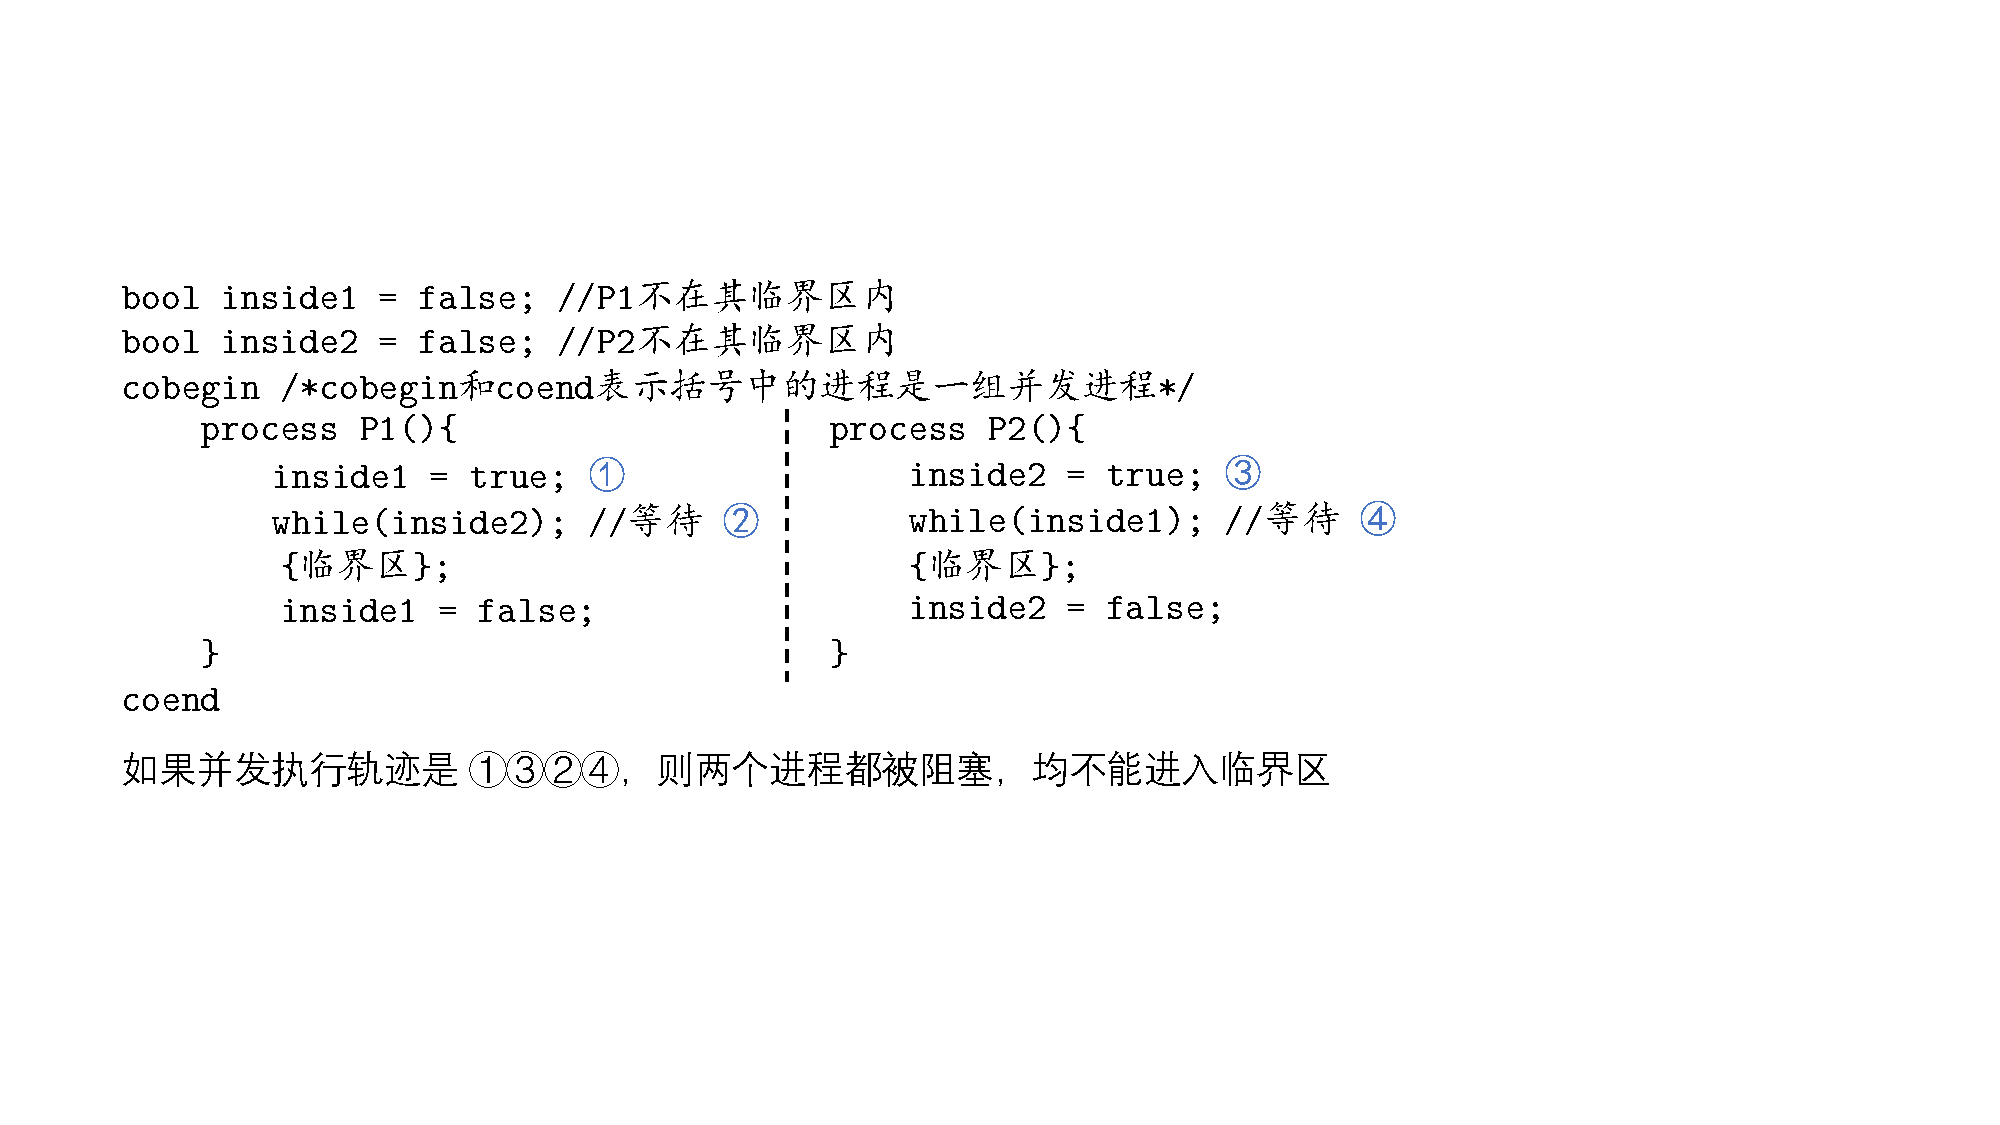
\includegraphics[width=0.8\textwidth]{img/临界区管理尝试2.pdf}
	\end{figure}

	解决算法:peterson算法,但该算法的通用性和效率较差
	\begin{figure}[H]
		\centering
		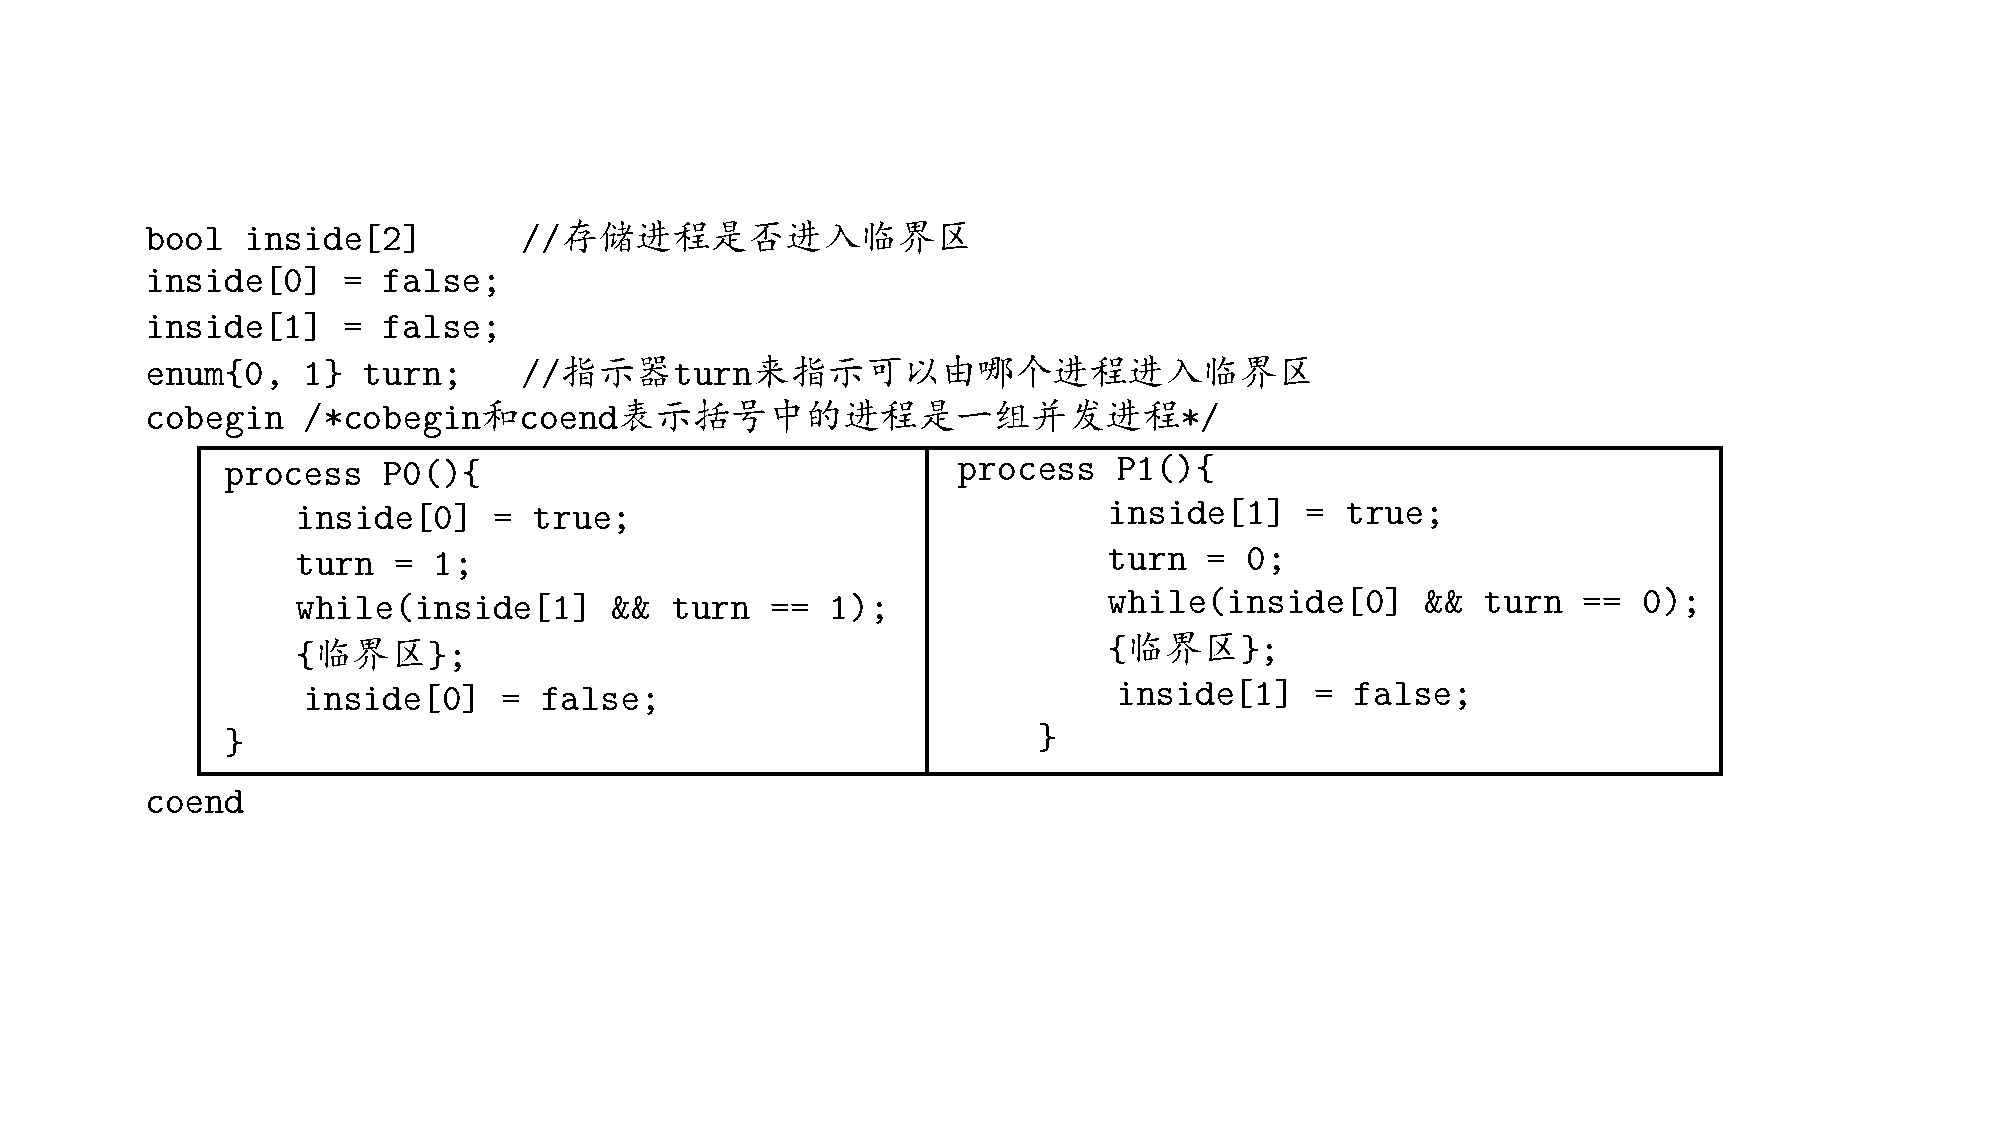
\includegraphics[width=0.8\textwidth]{img/peterson算法.pdf}
	\end{figure}

	\subsection{临界区管理的硬件方式}
	在单处理器计算机系统中,并发进程不能同时执行,只会交替地执行。为了保证互斥性,仅需保证进程不被中断。

	\subsubsection{关中断}
	实现互斥最简单的方法是在进程进入临界区时关中断,进程退出临界区时开中断。
	\begin{itemize}
		\item 由于进程上下文切换都是由中断事件引起的,因此关闭中断后进程的执行不会被打断
		\item 例如,Linux系统中采用内核函数cli() (clear interrupt)和 sti() (set
		interupt)实现关中断与开中断
		\item 操作系统原语就是基于该思路实现的,但该方式不适合作为通用的互斥机制
		\begin{itemize}
			\item 临界区的指令长度应短小精悍,否则关中断的时间过长会影响性能和系统效率
			\item 它不适用于多处理器系统,一个处理器关中断并不能防止进程在其他处理器上执行相同的临界区代码
			\item 若将这项权利赋予用户也存在危险,如果用户未开中断,则系统可能因此而终止
		\end{itemize}
	\end{itemize}

	\subsubsection{测试并设置(TS)指令}

	\begin{figure}[H]
		\centering
		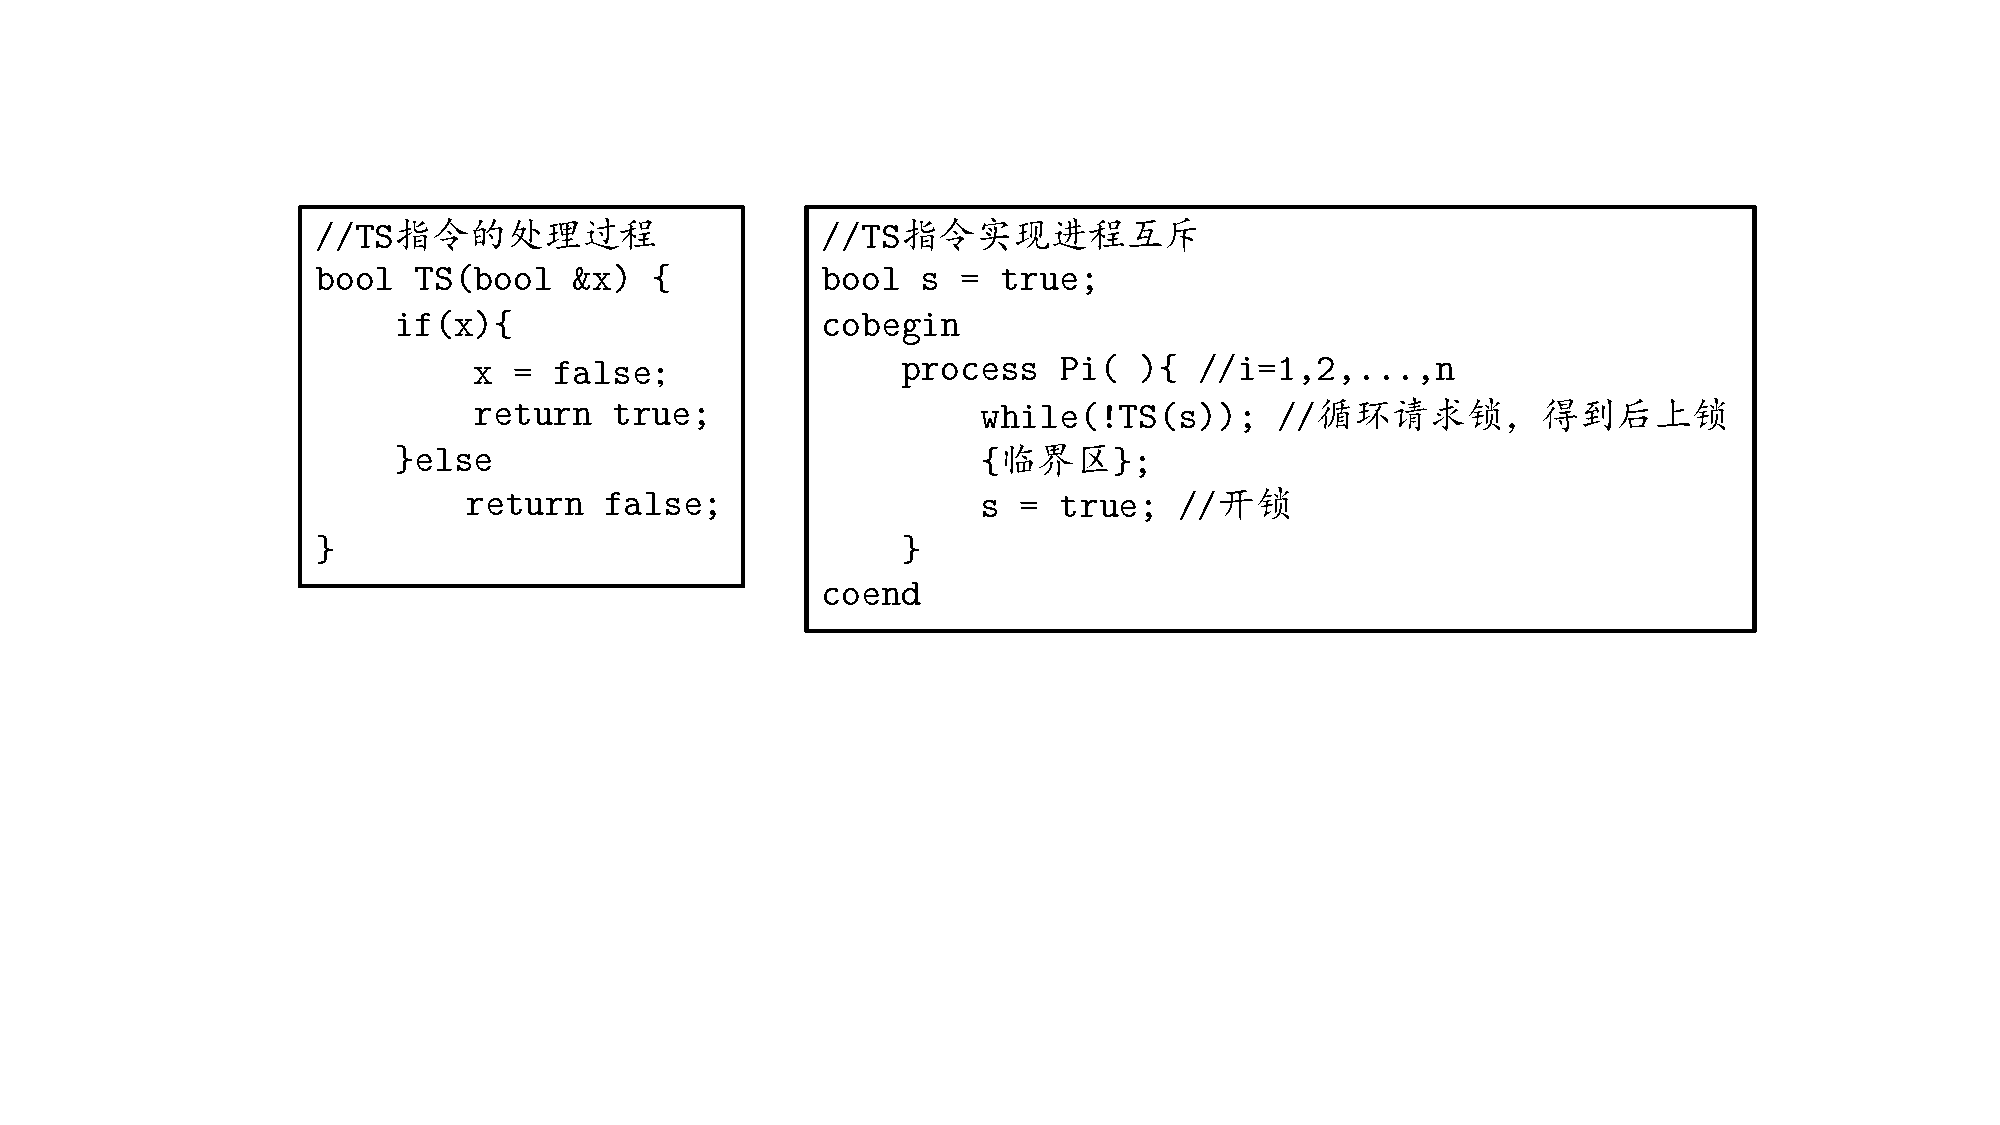
\includegraphics[width=0.7\textwidth]{img/TS指令.pdf}
	\end{figure}

	\subsubsection{对换指令}
	\begin{figure}[H]
		\centering
		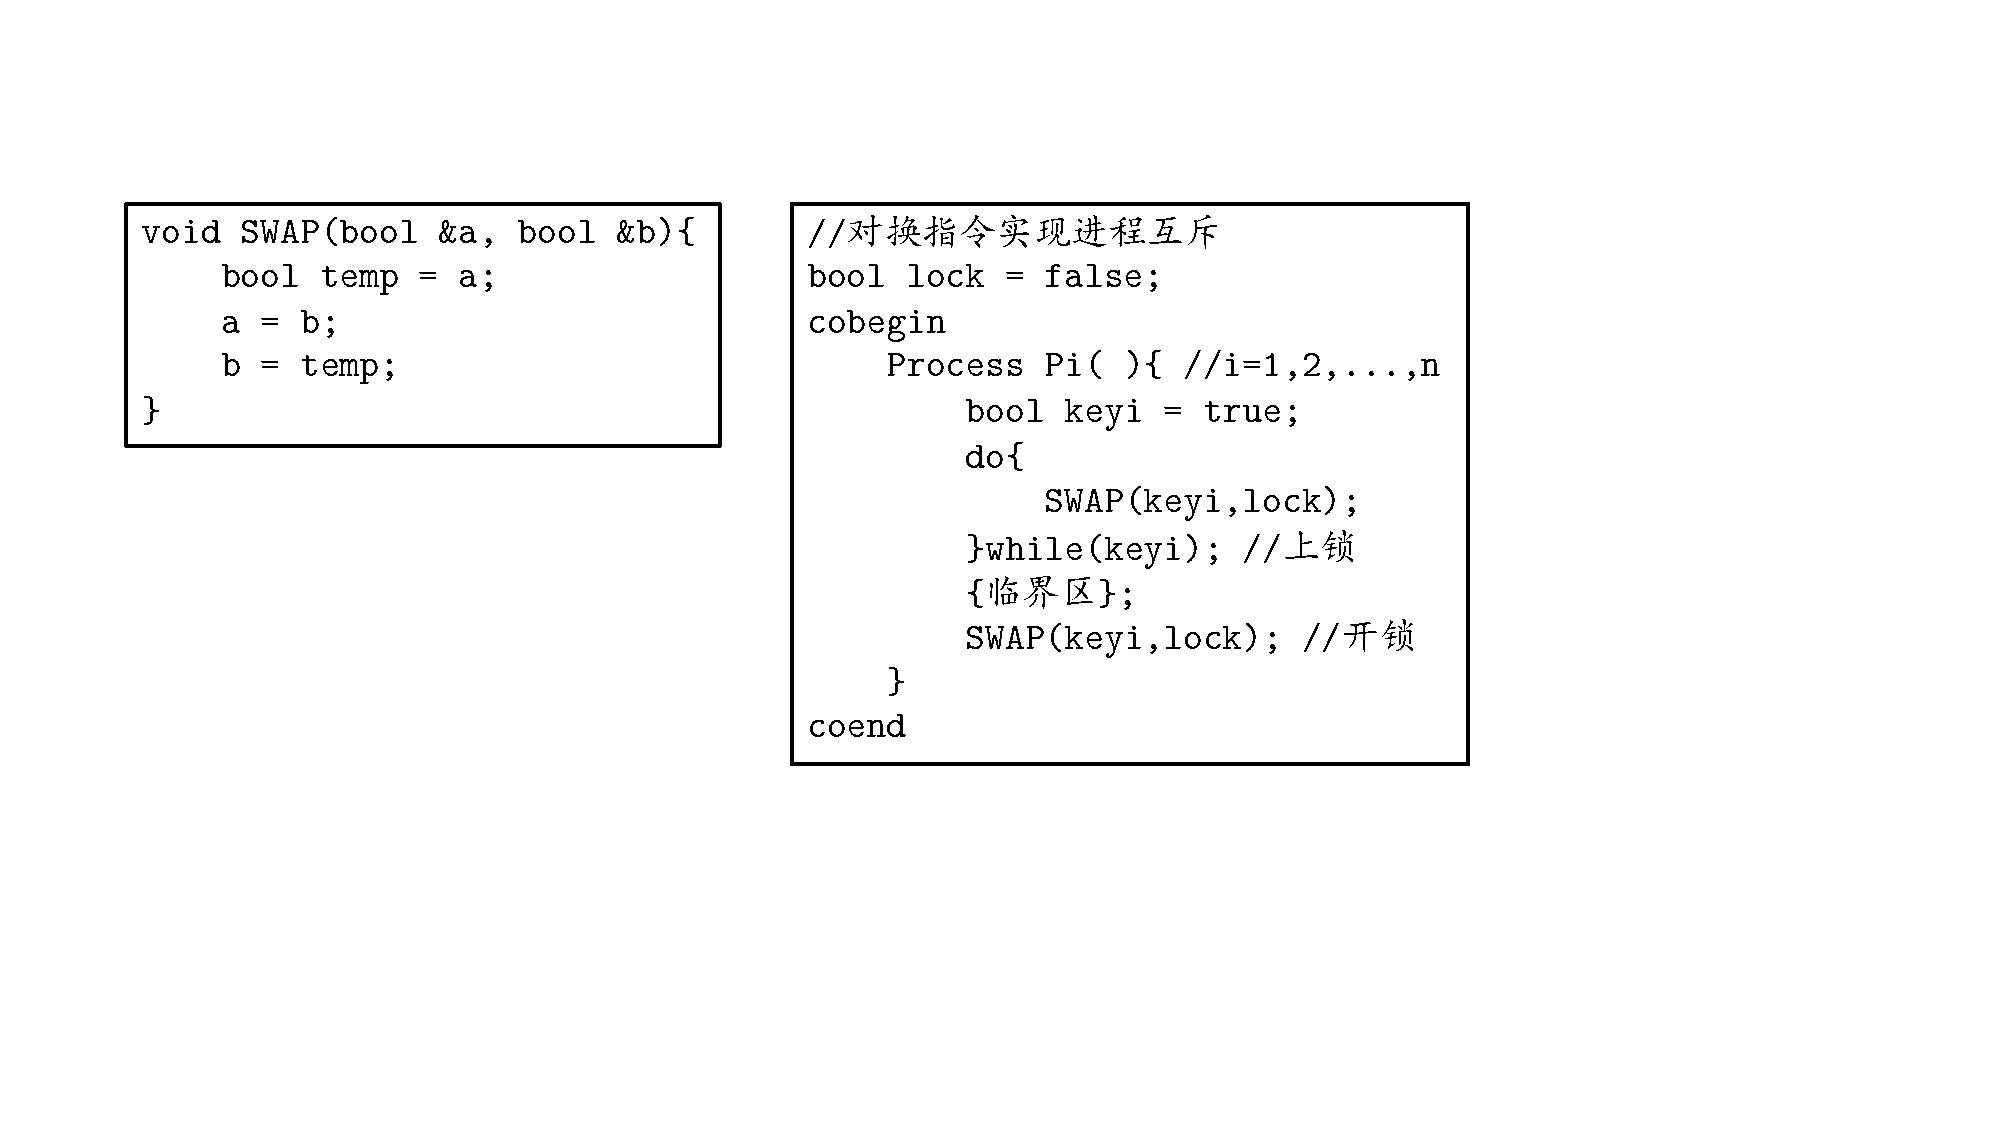
\includegraphics[width=0.7\textwidth]{img/对换指令.pdf}
	\end{figure}

	\section{PV操作}

	\subsection{PV操作与进程互斥}

	\subsubsection{PV操作}

	问题的提出:对于临界区管理的软硬件方法,虽然简单且行之有效,可以正确解决临界区调度问题,但也存在明
	显缺点:
	\begin{itemize}
		\item 软件算法太复杂,效率低下
		\item 硬件设施采用忙式等待测试,浪费CPU时间
		\item 将测试能否进入临界区的责任推给各个竞争的进程,削弱了系统的可靠性,加重了用户的编程负担
	\end{itemize}

	信号量是一种可动态定义的软件资源,其核心的数据结构就是让操作系统为它建立一个\textbf{等待进程队列}\begin{itemize}
		\item 信号量声明:当声明信号量并为其赋予一合理的初值时,相当于声明系统中可用的各类资源,操作系统就为可用的资源建立相关的等待队列
		\item 申请资源的原语:当申请资源时,如果申请结果是暂时得不到资源(或者是资源不满足),调用申请资源的原语就会将申请进程加入与该资源相关的等待队列中
		\item 释放资源的原语:当归还资源时,操作系统会检测在该资源的等待队列中有没有等待该资源的进程,如果有,便会将其释放
		\item 信号量的撤销:注销该信号量指代的资源,撤销与该信号量相关的队列
	\end{itemize}

	信号量的一种实现机制——记录型信号量在程序设计中的形式化定义
	\begin{lstlisting}[language=C,keywordstyle=\color{black}]
typedef struct semaphore{
	int value;			/* 信号量值 */
	struct pcb * list;	/* 信号量等待进程队列指针 */
}
	\end{lstlisting}
	\begin{itemize}
		\item value为整型变量,系统初始化时为其赋值
		\begin{itemize}
			\item 正值表示资源可复用次数
			\item 0值表示无资源且无进程等待
			\item 负值表示等待队列中进程个数
		\end{itemize}
		\item list是等待使用此类资源的进程队列的头指针,初始状态为空队列
	\end{itemize}

	设s为一个记录型信号量,关于s的PV操作原语描述如下:
	\begin{itemize}
		\item P(s):将信号量s的value值减1
		\begin{itemize}
			\item 若结果小于0,则执行P操作的进程被阻塞,进入信号量s的list所指队列中
			\item 若结果大于等于0,则执行操作的进程继续执行
		\end{itemize}
		\item V(s):将信号量s的value值加1
		\begin{itemize}
			\item 若结果不大于0,则执行V操作的进程从信号量s的list 所指队列中释放一个进程,使其转换为就绪态,自己则继续执行
			\item 若结果大于0,则执行V操作的进程继续执行
		\end{itemize}
	\end{itemize}

	将PV操作定义为如下不可中断过程
	\begin{lstlisting}[language=C,keywordstyle=\color{black}]
// P操作原语
void P(semaphore s) {
	s.value--;           /* 信号量值减1 */
	if(s.value < 0)
		sleep(s.list);
/* 
*   若信号量值小于0,执行P操作的进程调用sleep(s.list)阻塞自己,被置成等待信号量s状态并移入s信号量队列,转向进程调度程序 
*/
}
	\end{lstlisting}

	\begin{lstlisting}[language=C,keywordstyle=\color{black}]
// V操作原语
void V(semaphore s) {
	s.value++;           /* 信号量值加1 */
	if(s.value <= 0)
		wakeup(s.list) ;
/* 
*   若信号量值小于等于0,则调用wakeup(s.list)从信号量s队列中释放一个等待信号量s的进程并转换成就绪态,进程则继续执行 
*/  
}		
	\end{lstlisting}

	信号量与进程状态转换模型
	\begin{figure}[H]
		\centering
		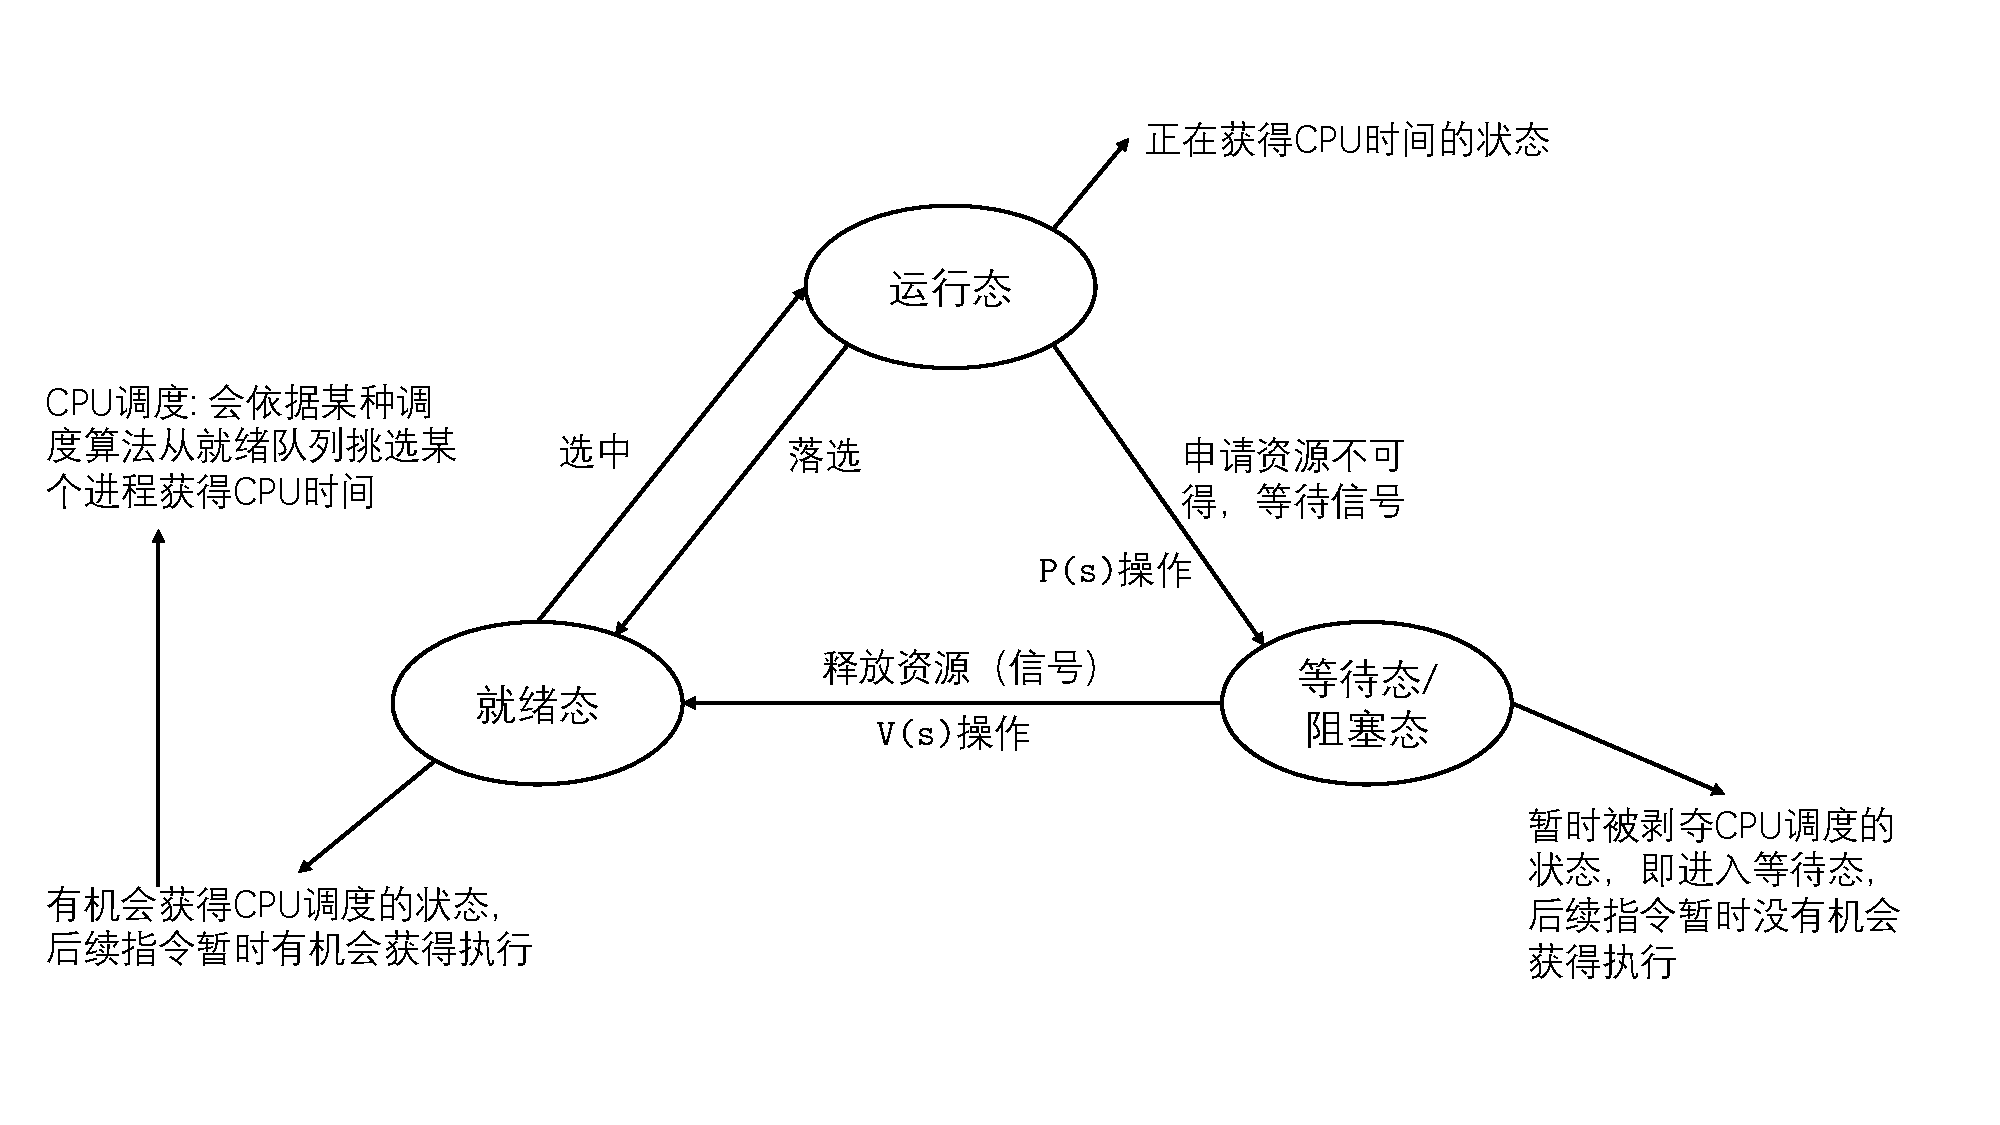
\includegraphics[width=0.8\textwidth]{img/信号量与进程状态转换模型.pdf}
	\end{figure}

	信号量与进程队列模型
	\begin{figure}[H]
		\centering
		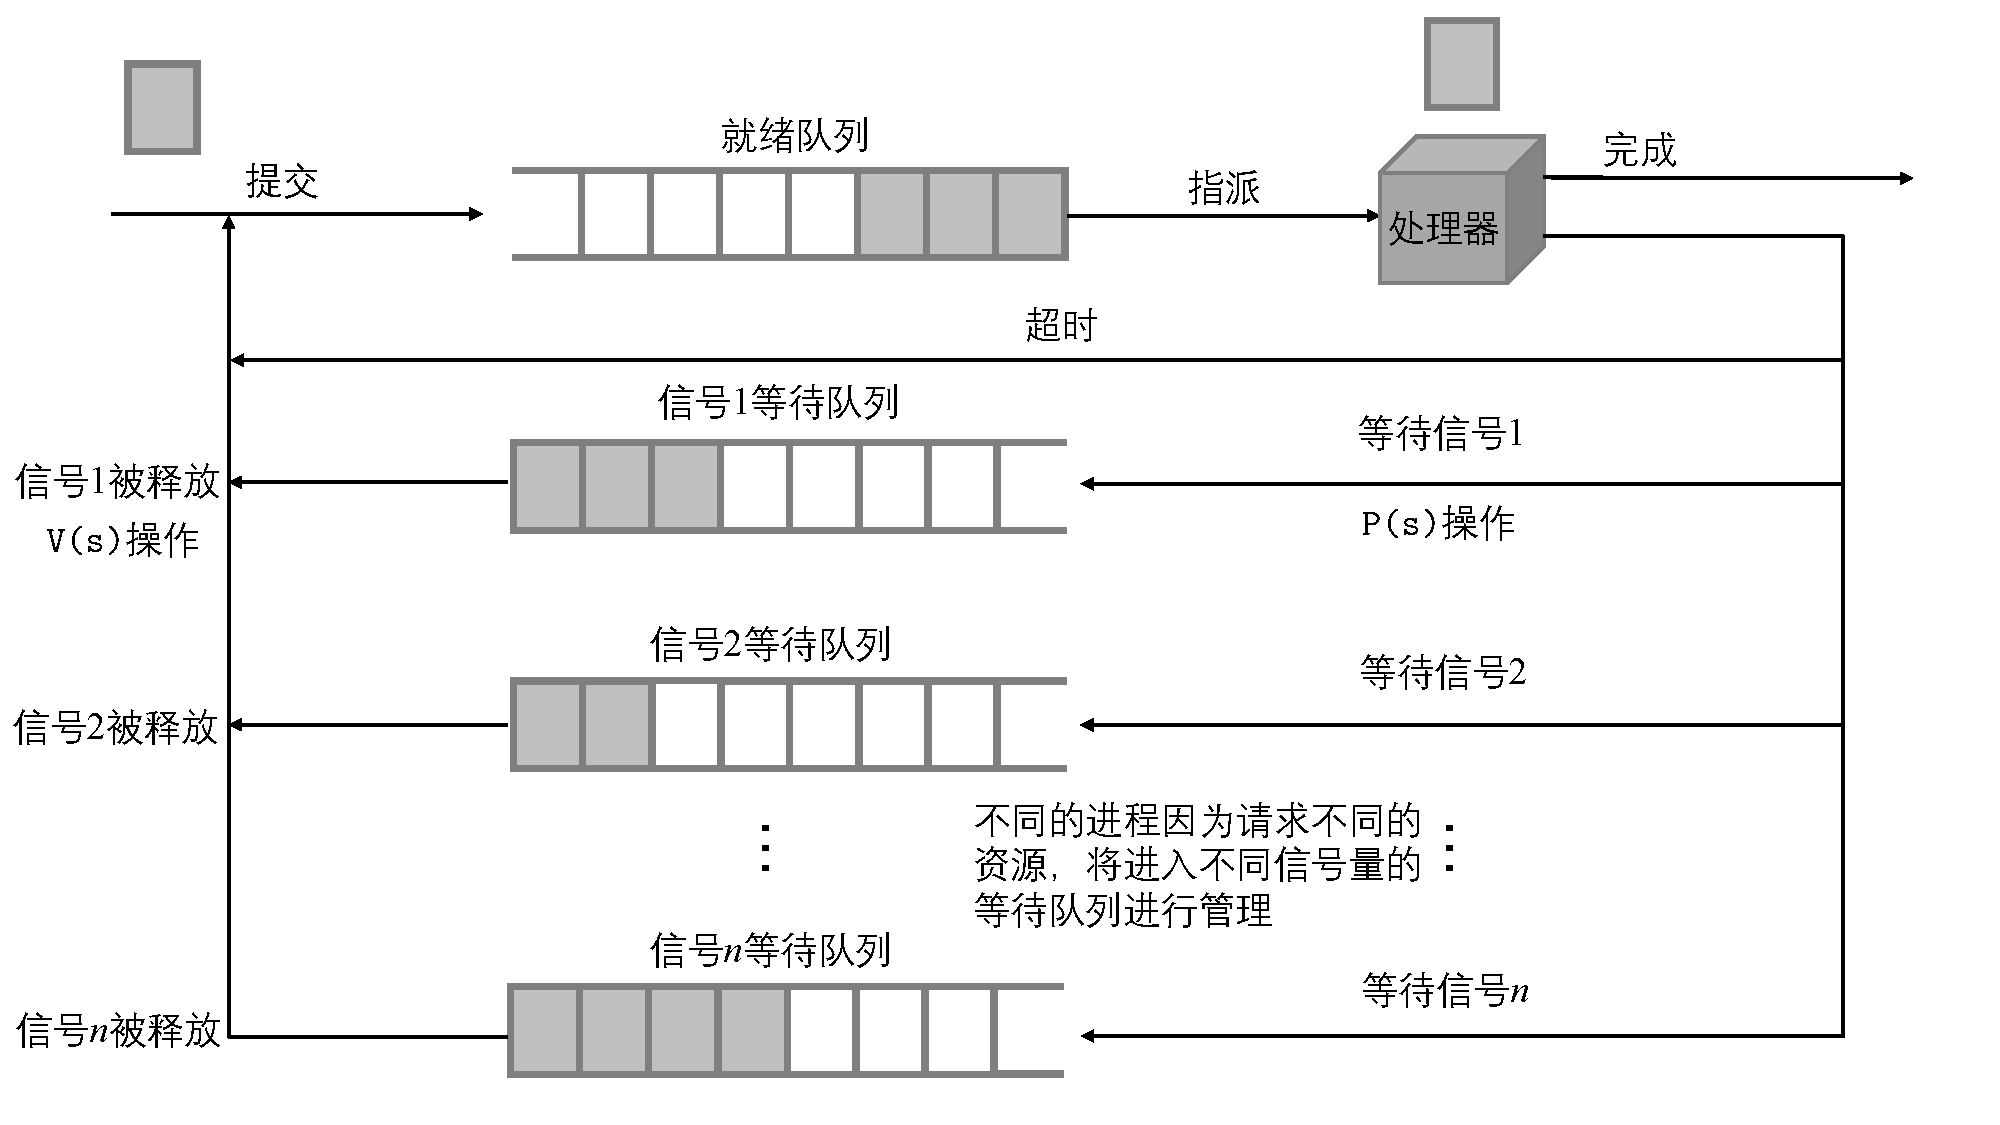
\includegraphics[width=0.8\textwidth]{img/信号量与进程队列模型.pdf}
	\end{figure}

	信号量与PV操作的推论
	\begin{itemize}
		\item 若信号量s的value值为正值,此值等于在封锁进程之前对信号量s可施行的P操作数,即s.value 代表实际可用的物理资源数。
		\item 若信号量s的value值为负值,其绝对值等于登记排列在信号量s的list所指队列中等待进程的个数,即等于对信号量s实施P操作而被封锁并进入信号量s等待队列的进程数。
		\item P操作通常意味着请求一个资源,V操作意味着释放一个资源。在一定条件下,P操作代表阻塞进程的操作,而V操作代表唤醒被阻塞进程的操作。
	\end{itemize}

	\subsubsection{PV操作解决进程互斥问题}
	使用信号量与PV操作管理并发进程互斥进入临界区的一般形式如下
	\begin{lstlisting}[language=C, keywordstyle=\color{black}]
semaphore s = 1;
cobegin
	Process Pi(){ 	/* i=1,…,n */
		...
		P(s); 		//申请进入临界区
		{临界区};
		V(s); 		//申请退出临界区
		...
	};
coend		
	\end{lstlisting}

	在表达纯粹互斥关系时信号量初值为1,且同一个信号量的P操作和V操作处于同一侧进程之中,但是这种情形不适用于同步关系

	\begin{figure}[H]
		\centering
		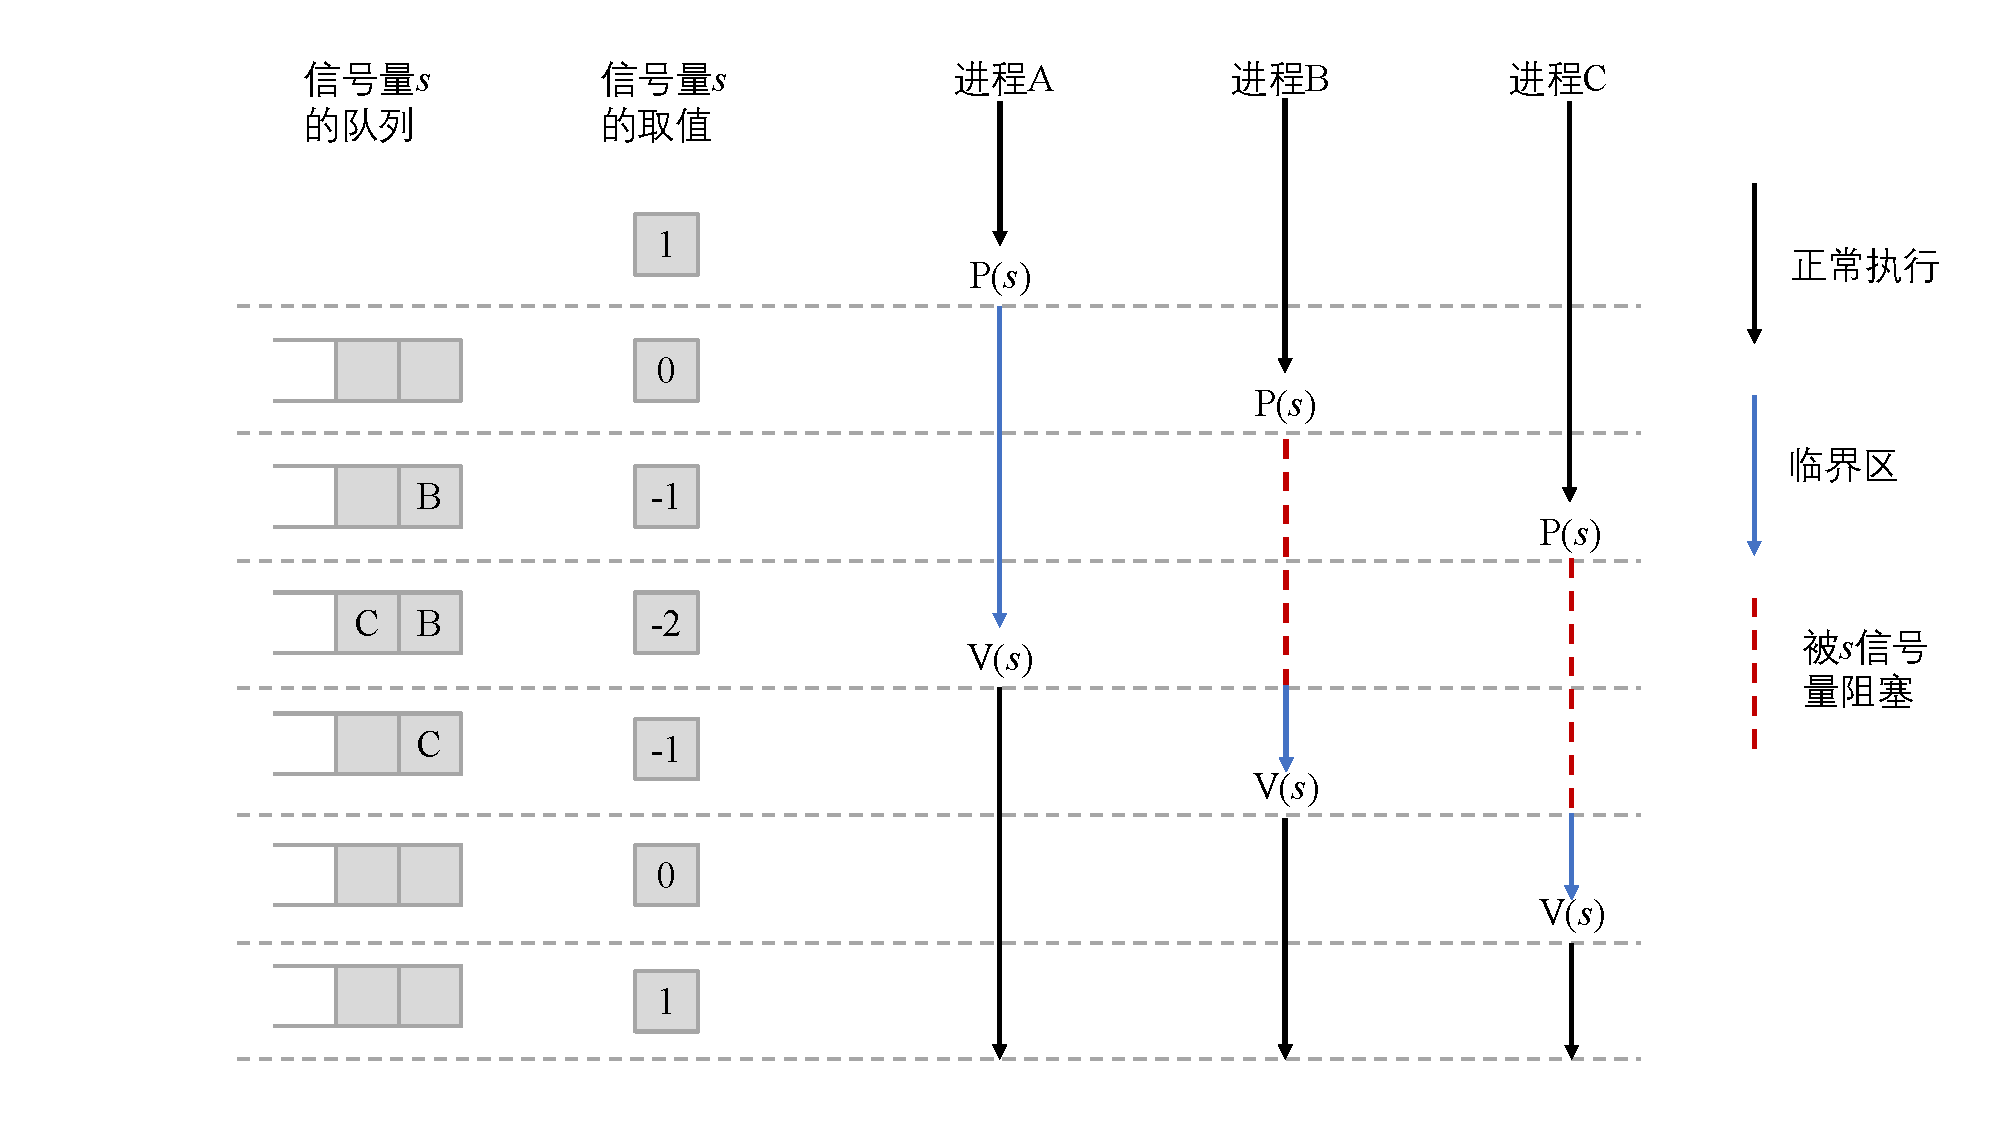
\includegraphics[width=0.8\textwidth]{img/信号量与PV操作控制并发进程之间的临界资源.pdf}
	\end{figure}

	\paragraph{飞机售票问题}~{}

	用记录型信号量与PV操作解决飞机售票问题
\begin{lstlisting}[language=C, keywordstyle=\color{black}]
int A[m];
semaphore s;
s = 1;
cobegin
	process Pi(){
		int Xi;
		L1: 按旅客订票要求找到A[j];
		P(s);
		Xi = A[j];
		if (Xi >= 1){
			Xi = Xi - 1;
			A[j] = Xi;
			V(s);
			{输出一张票};
		}else{
			V(s);
			{输出票已售完};
		}
	   goto L1;
	}
coend
\end{lstlisting}

	对于上述问题而言,只有相同航班的票数才是相关的临界资源,所以用一个信号量处理全部机票的销售过程会影响进程并发度

	因此对以上程序做出改进:为每一个航班定义一个信号量,可以定义一个信号量数组,即每一个航班都有其各自的临界区

	\begin{lstlisting}[language=C, keywordstyle=\color{black}]
int A[m];
semaphore s[m];
for (int i = 0; i < m; i++){
	s[i] = 1;
}
cobegin
	process Pi(){
		int Xi;
		L1: 按旅客订票要求找到A[j];
		P(s[j]);
		Xi = A[j];
		if (Xi >= 1){
			Xi = Xi - 1;
			A[j] = Xi;
			V(s[j]);
			{输出一张票};
		}else{
			V(s[j]);
			{输出票已售完};
		}
		goto L1;
	}
coend
	\end{lstlisting}

	\paragraph{哲学家就餐问题}~{}

	问题描述:有五个哲学家围坐在一圆桌旁,桌中央有一盘通心面,每人面前有一只空盘子,每两人之间放一把叉子。每个哲学家思考、饥饿、然后吃通心面。为了吃面,每个哲学家必须获得两把叉子,且每人只能直接从自己左边或右边去取叉子

	\begin{figure}[H]
		\centering
		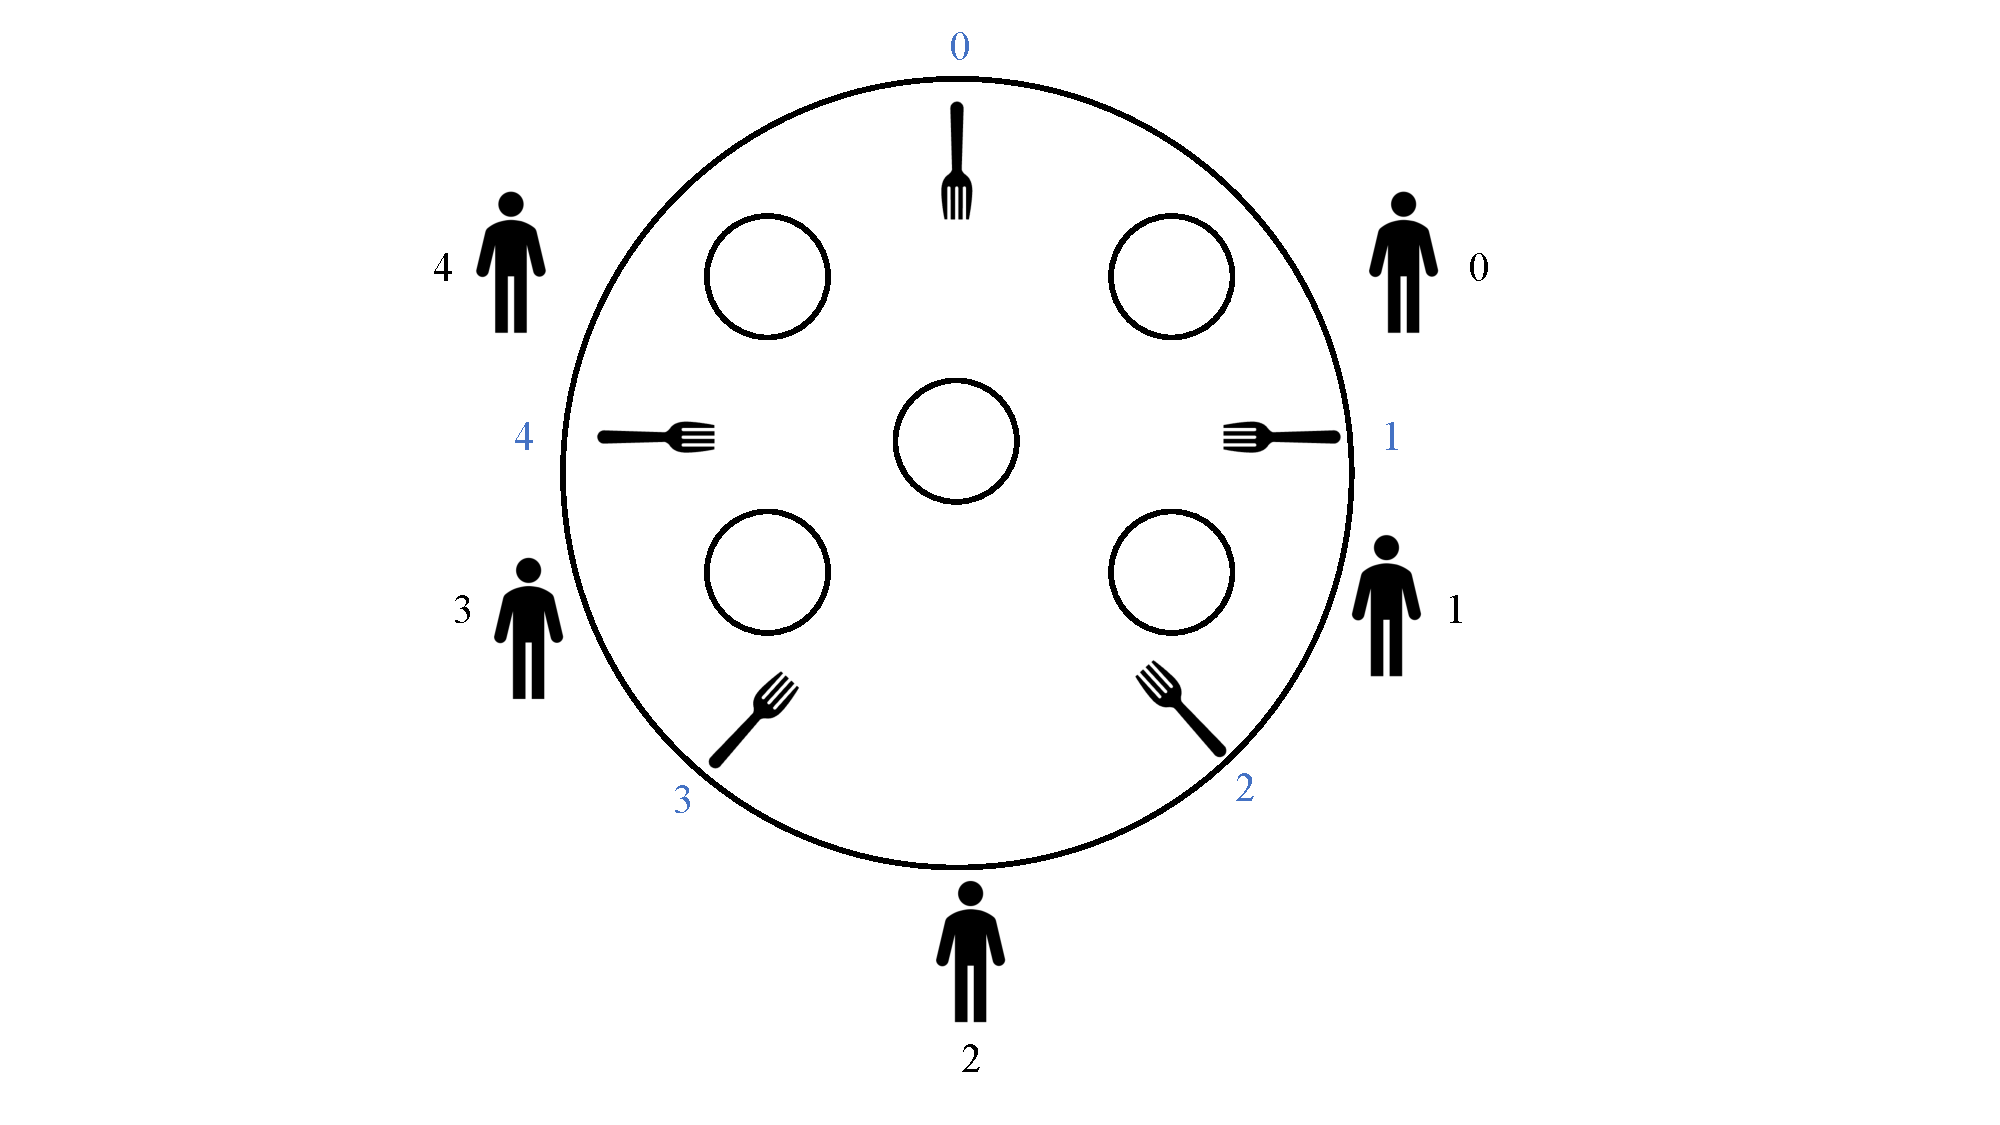
\includegraphics[width=0.4\textwidth]{img/哲学家就餐问题描述.pdf}
	\end{figure}

	\begin{lstlisting}[language=C, keywordstyle=\color{black}]
//存在死锁的哲学家就餐问题
semaphore fork[5];
for (int i = 0; i < 5; i++){
	fork[i] = 1;
}
cobegin
	process philosopher_i( ) { //i=0,1,2,3,4
		while(true) {
			think();
			P(fork[i]); 		//先取右手的叉子
			P(fork[(i+1)%5]); 	//再取左手的叉子
			eat();
			V(fork[i]);
			V(fork[(i+1)%5]);
		}
	}
coend	
	\end{lstlisting}
	上面的代码存在死锁的问题:比如当每一个哲学家都拿到了一侧的叉子将出现死锁,有若干种办法可避免死锁
	\begin{itemize}
		\item 至多允许四个哲学家同时取叉子(C.A.R.Hoare方案)
		\item 奇数号的哲学家先取左手边的叉子,偶数号的哲学家先取右手边的叉子
	\end{itemize}

	“至多允许四个哲学家同时取叉子”的解决办法

	\begin{lstlisting}[language=C, keywordstyle=\color{black}]
//设置侍者,添加房间信号量来控制同时取叉子的哲学家个数
semaphore fork[5];
for (int i = 0; i < 5; i++){
	fork[i] = 1;
}			  
semaphore room = 4; //增加一个侍者,设想有两个房间,1号房间是会议室,2号房间是餐厅
cobegin
	process philosopher_i(){ /*i=0,1,2,3,4 */
		while(true) {
			think();
			P(room); //控制最多允许4位哲学家进入2号房间餐厅取叉子
			P(fork[i]);
			P(fork[(i+1)%5]) ;
			eat();
			V(fork[i]);
			V(fork[(i+1)%5]);
			V(room);
		}
	}
coend		
	\end{lstlisting}

	“奇数号的哲学家先取左手边的叉子,偶数号的哲学家先取右手边的叉子”的解决办法
	\begin{lstlisting}[language=C, keywordstyle=\color{black}]
//限制奇数号的哲学家优先取左手边的叉子,偶数号的哲学家优先取右手边的叉子
void philosopher(int i){
	if (i % 2 == 0){
		P(fork[i]);         //偶数哲学家先取右手边的叉子
		P(fork[(i+1)%5]);   //后取左手边的叉子
		eat();
		V(fork[i]);
		V(fork[(i+1)%5]);
	}else{
		P(fork[(i+1)%5]);  //奇数号哲学家先取左手边的叉子
		P(fork[i]);        //后取右手边的叉子
		eat();
		V(fork[(i+1)%5]);
		V(fork[i]);
	}
}
	\end{lstlisting}

	\subsection{PV操作与进程同步}
	
	\subsubsection{PV操作解决进程同步问题的基本思路}
	使用信号量与PV操作解决进程同步问题的基本思路如下:
	\begin{itemize}
		\item 定义一个记录型信号量,用于表示可用的消息数(资源数)
		\item 等待消息的进程在执行P操作后,如果没有得到消息,它就会被阻塞在同步信号量的等待队列,并依序排队
		\item 发出消息的进程在执行V操作后,如果有等待该消息的进程,它将唤醒一个在该同步信号量上等待的进程
	\end{itemize}

	\subsubsection{生产者消费者问题}
	问题描述:有$n$个生产者和$m$个消费者,连接在一个有$k$个单位缓冲区的有界缓冲上。其中,生产者进程\ \verb|Producer_i|\ 和消费者进程\ \verb|Consumer_j|\ 都是并发进程,只要缓冲区未满,生产者\ \verb|Producer_i|\ 生产的产品就可投入缓冲区;只要缓冲区不空,消费者进程\ \verb|Consumer_j|\ 就可从缓冲区取走并消耗产品

	可能的情形有:
	\begin{itemize}
		\item $n=1,m=1,k=1$
		\item $n=1,m=1,k>1$
		\item $n>1,m>1,k>1$
	\end{itemize}

	\paragraph{生产者消费者问题分析}~{}

	\begin{figure}[H]
		\centering
		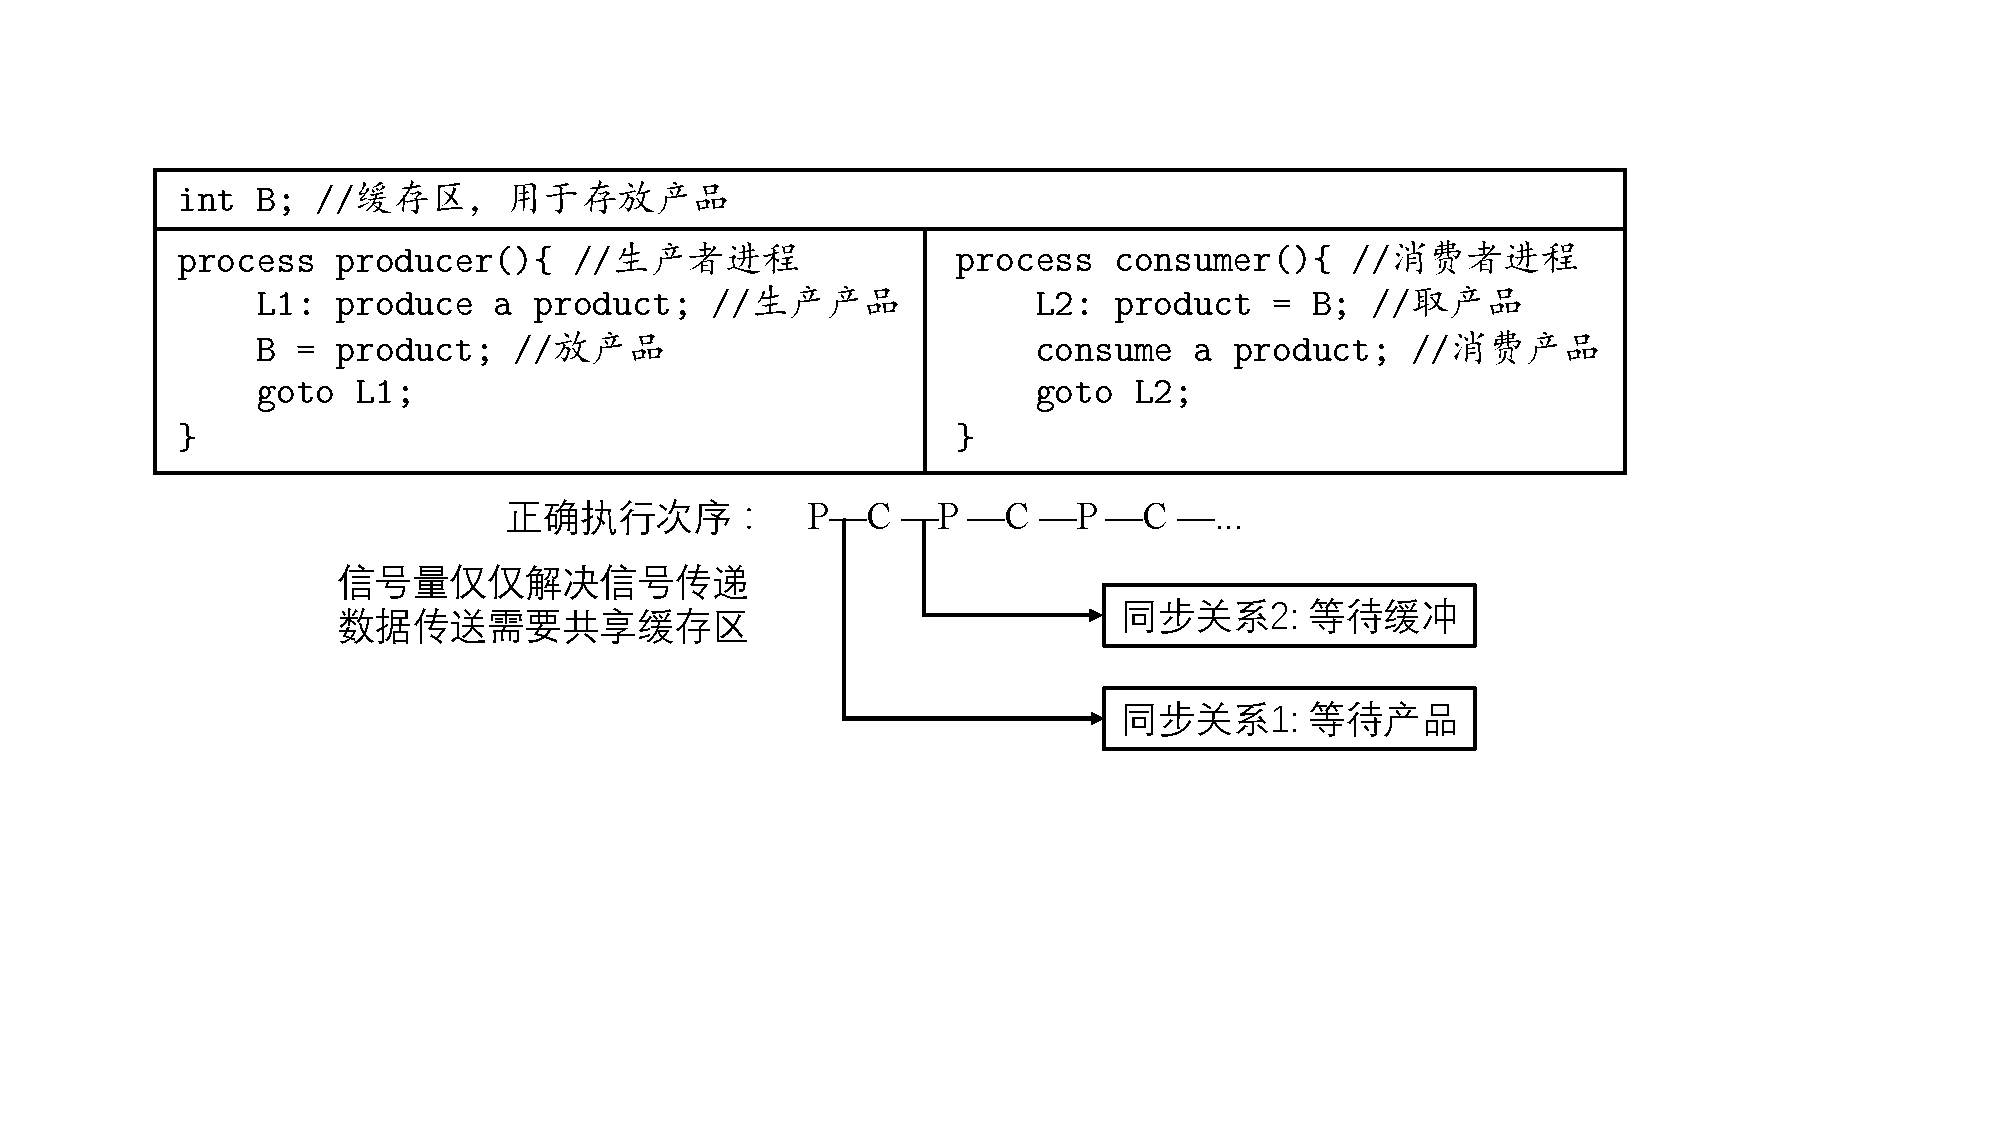
\includegraphics[width=0.9\textwidth]{img/生产者-消费者问题的程序框架.pdf}
	\end{figure}

	生产者和消费者共享缓冲区
	\begin{itemize}
		\item 缓冲区有空位时,生产者可放入产品,否则等待
		缓冲区有产品时,消费者可取出产品,否则等待
	\end{itemize}

	同步问题的解决思路
	\begin{itemize}
		\item 同步关系1:对于消费者,设置一个同步信号量sget等待产品。在初始状态时,缓冲区为空,因此该同步信号量的初始值为0。V(sget)操作位于生产者进程中,表示产品己放置在缓冲区中;P(sget)位于消费者进程中,表示需要等待生产者填入产品
		\item 同步关系2:设置另一信号量sput,表示等待缓冲区为空。在初始状态时,缓冲区为空,因此该同步信号量的初始值为1,即生产者初始时可以放进一件产品。P(sput)操作位于生产者进程中,表示需要等待缓冲区为空时才能生产产品;V(sput)位于消费者进程,表示消费者已取出缓冲区中的产品。
	\end{itemize}

	\paragraph{一个生产者、一个消费者共享一个缓冲区问题}~{}

	\begin{figure}[H]
		\centering
		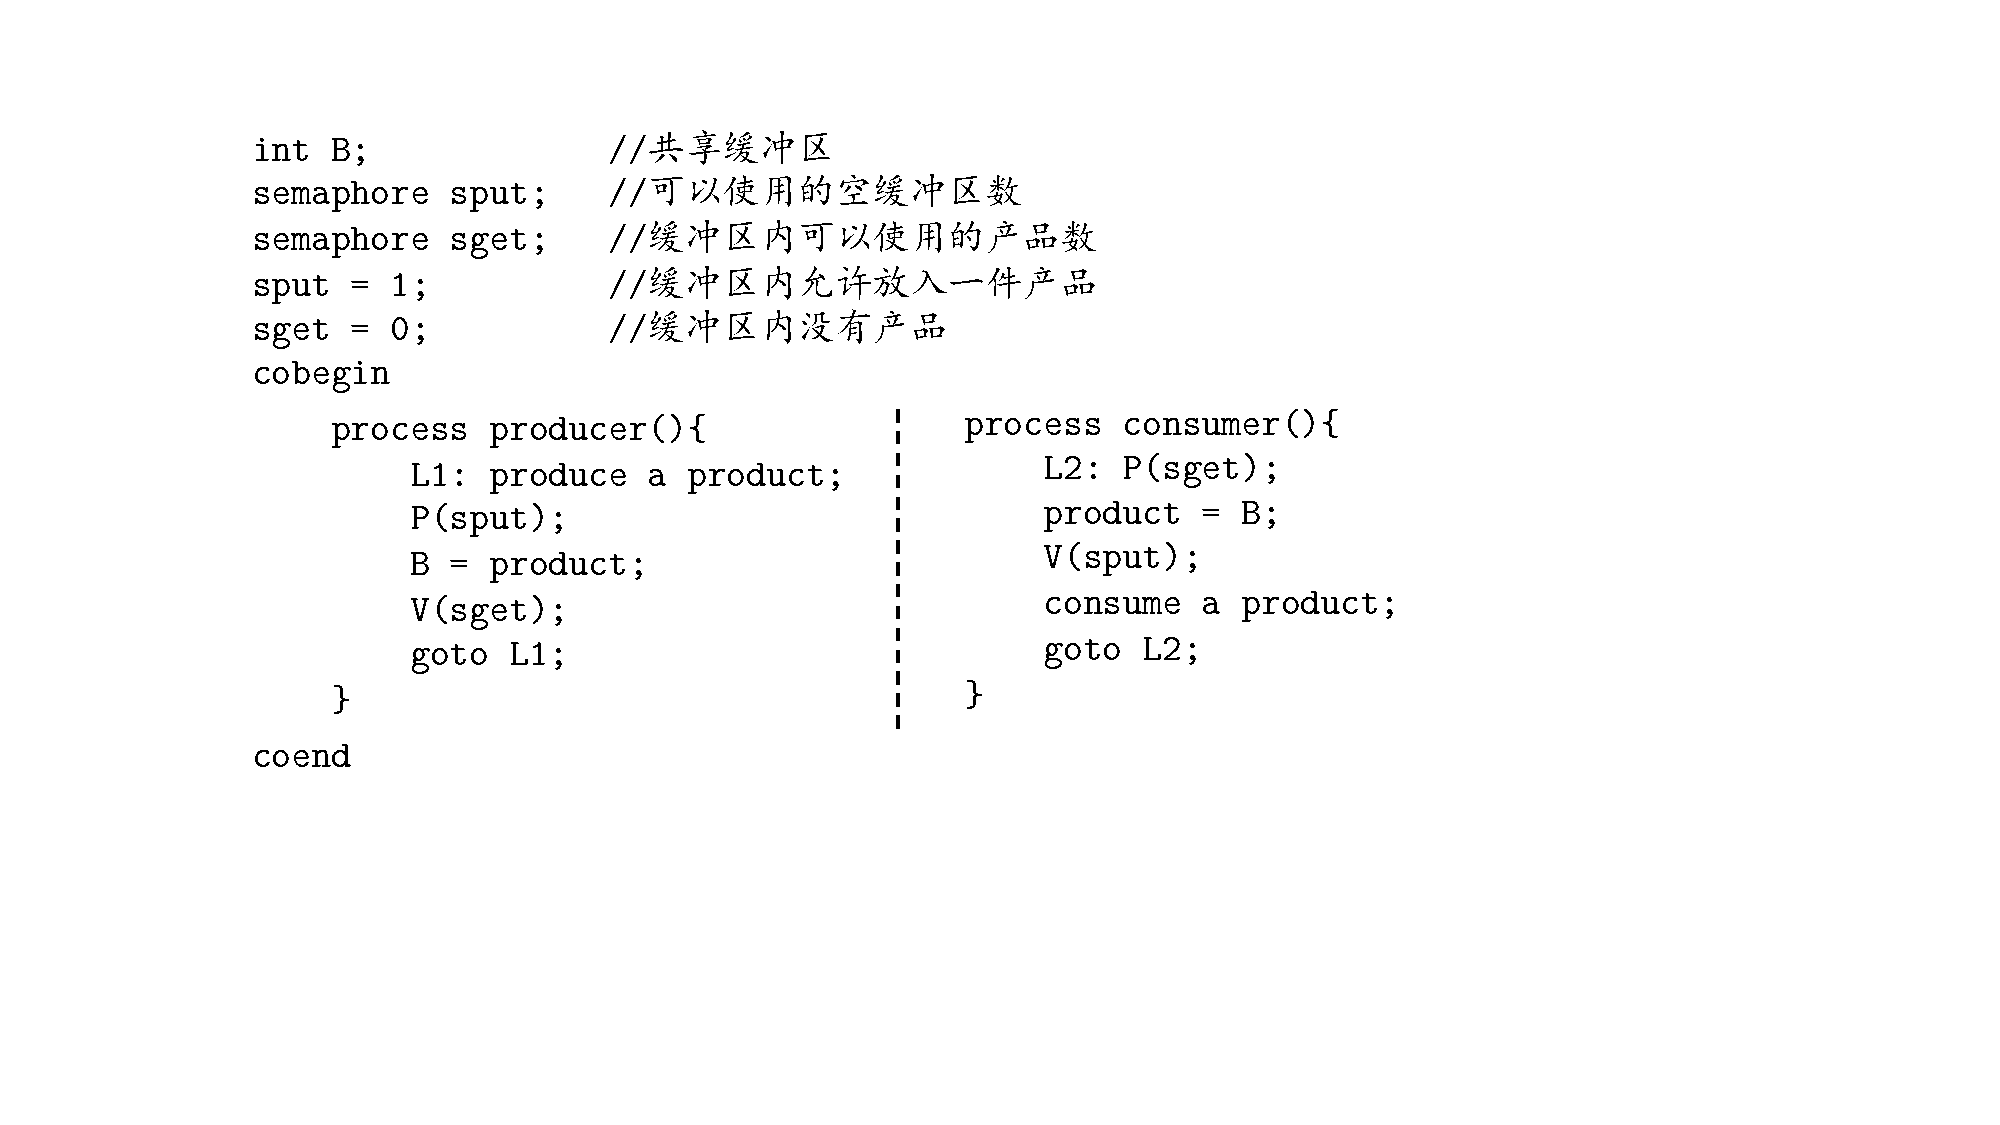
\includegraphics[width=0.65\textwidth]{img/一个生产者、一个消费者共享一个缓冲区问题.pdf}
	\end{figure}

	\paragraph{一个生产者、一个消费者共享多个缓冲区问题}~{}

	\begin{figure}[H]
		\centering
		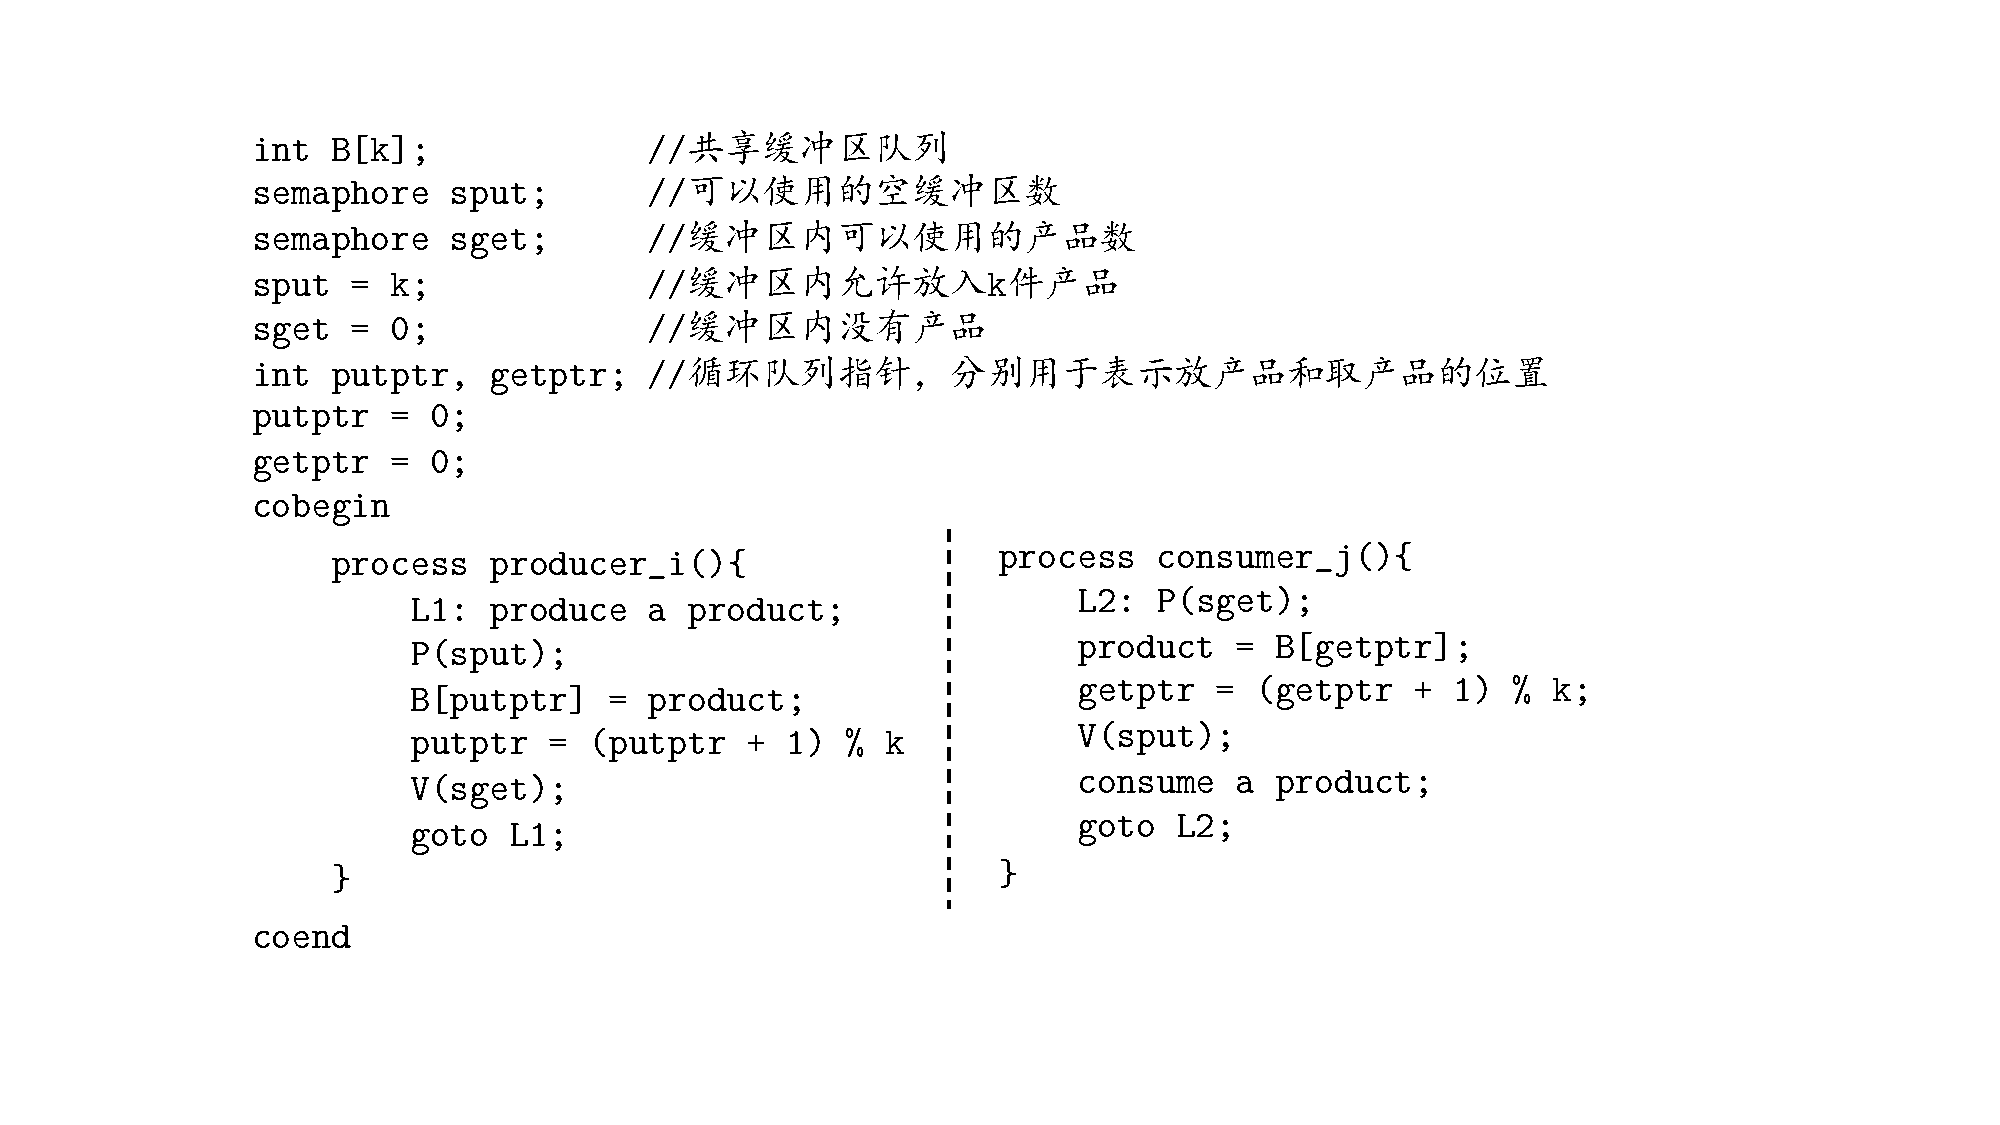
\includegraphics[width=0.85\textwidth]{img/一个生产者、一个消费者共享多个缓冲区问题.pdf}
	\end{figure}

	\paragraph{多个生产者、多个消费者共享多个缓冲区问题}~{}

	\begin{figure}[H]
		\centering
		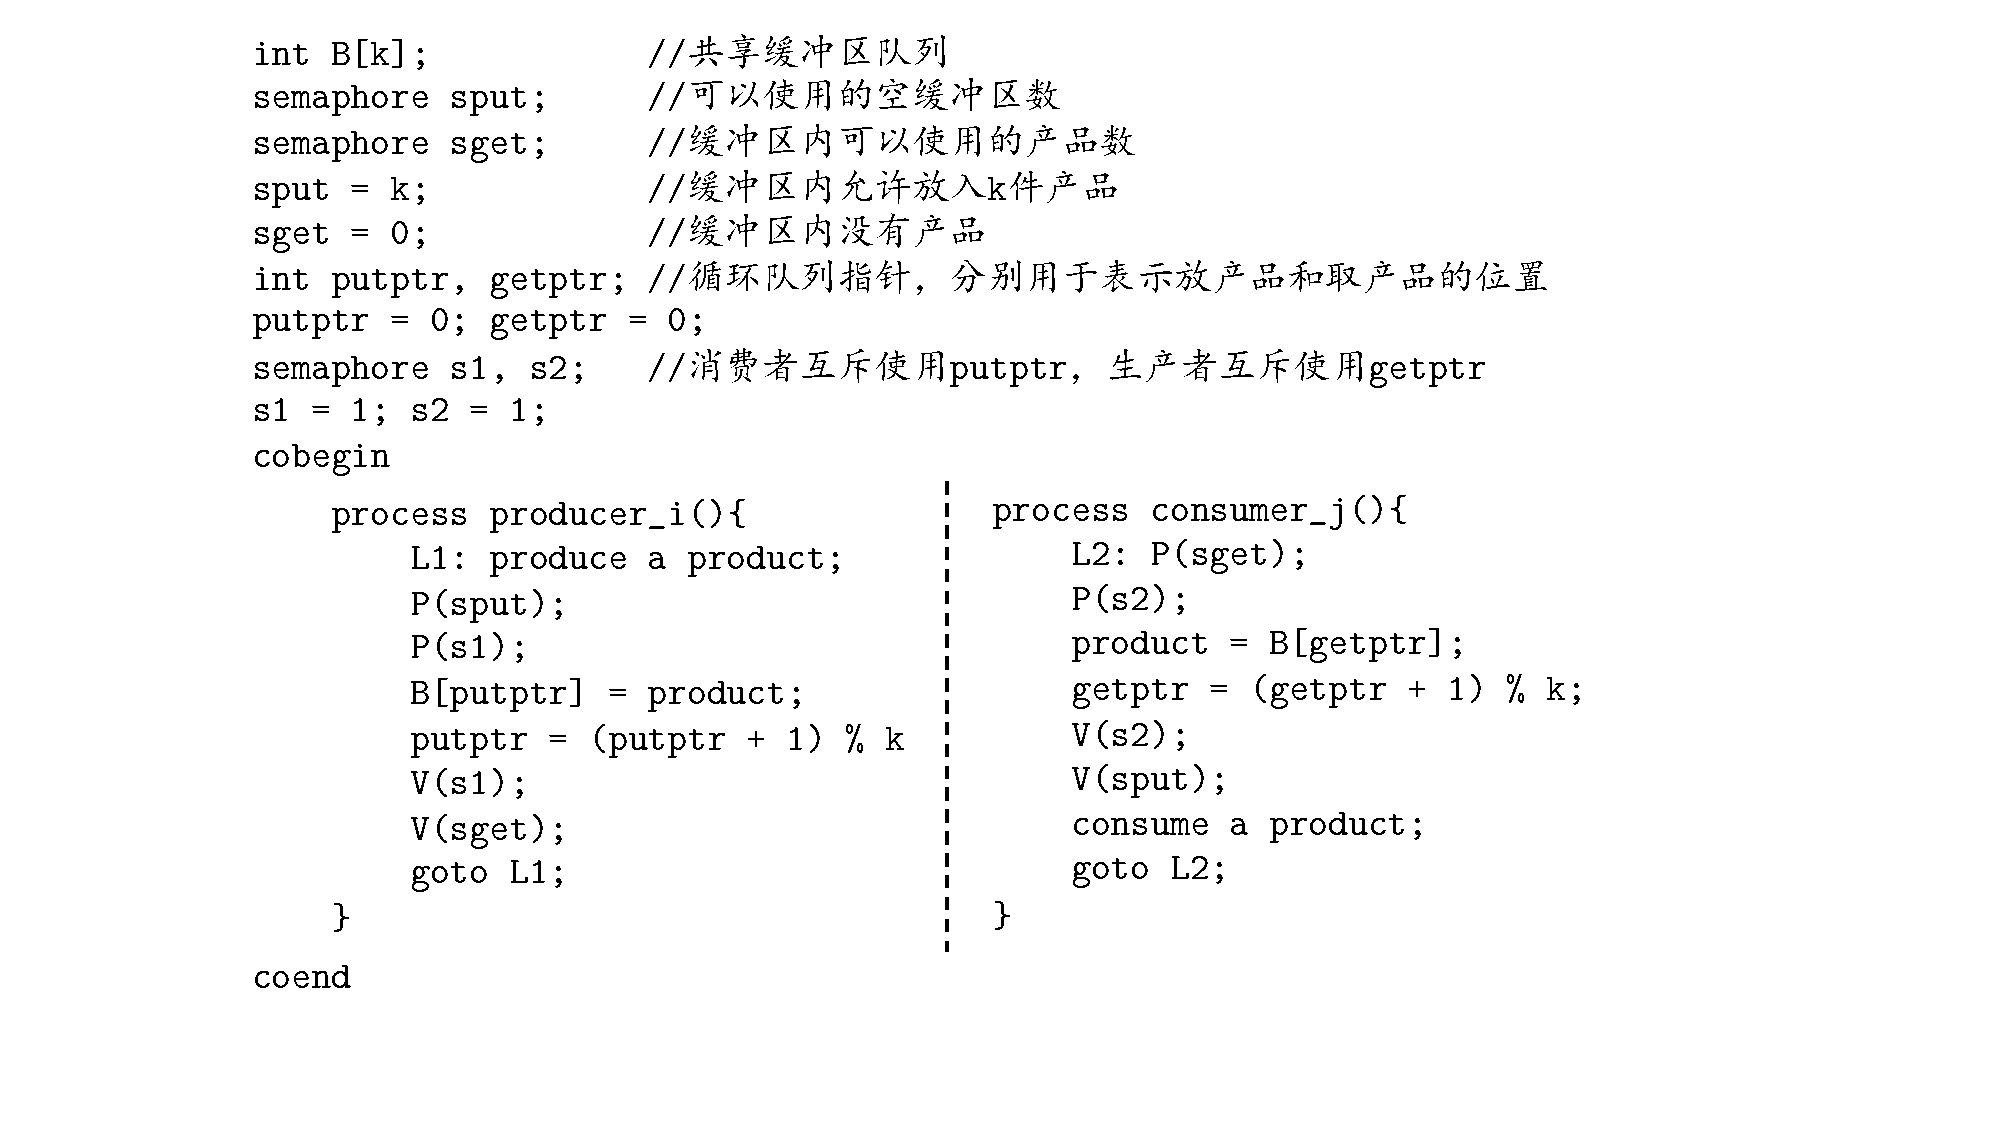
\includegraphics[width=0.85\textwidth]{img/多个生产者、多个消费者共享多个缓冲区问题.pdf}
	\end{figure}

	\subsubsection{苹果-橘子问题}
	问题描述:桌上有一只盘子,每次只能放入一个水果。爸爸专门向盘子中放苹果,妈妈专门向盘子中放橘子,一个儿子专门等着吃盘子中的橘子,一个女儿专门等着吃盘子中的苹果。

	\begin{figure}[H]
		\centering
		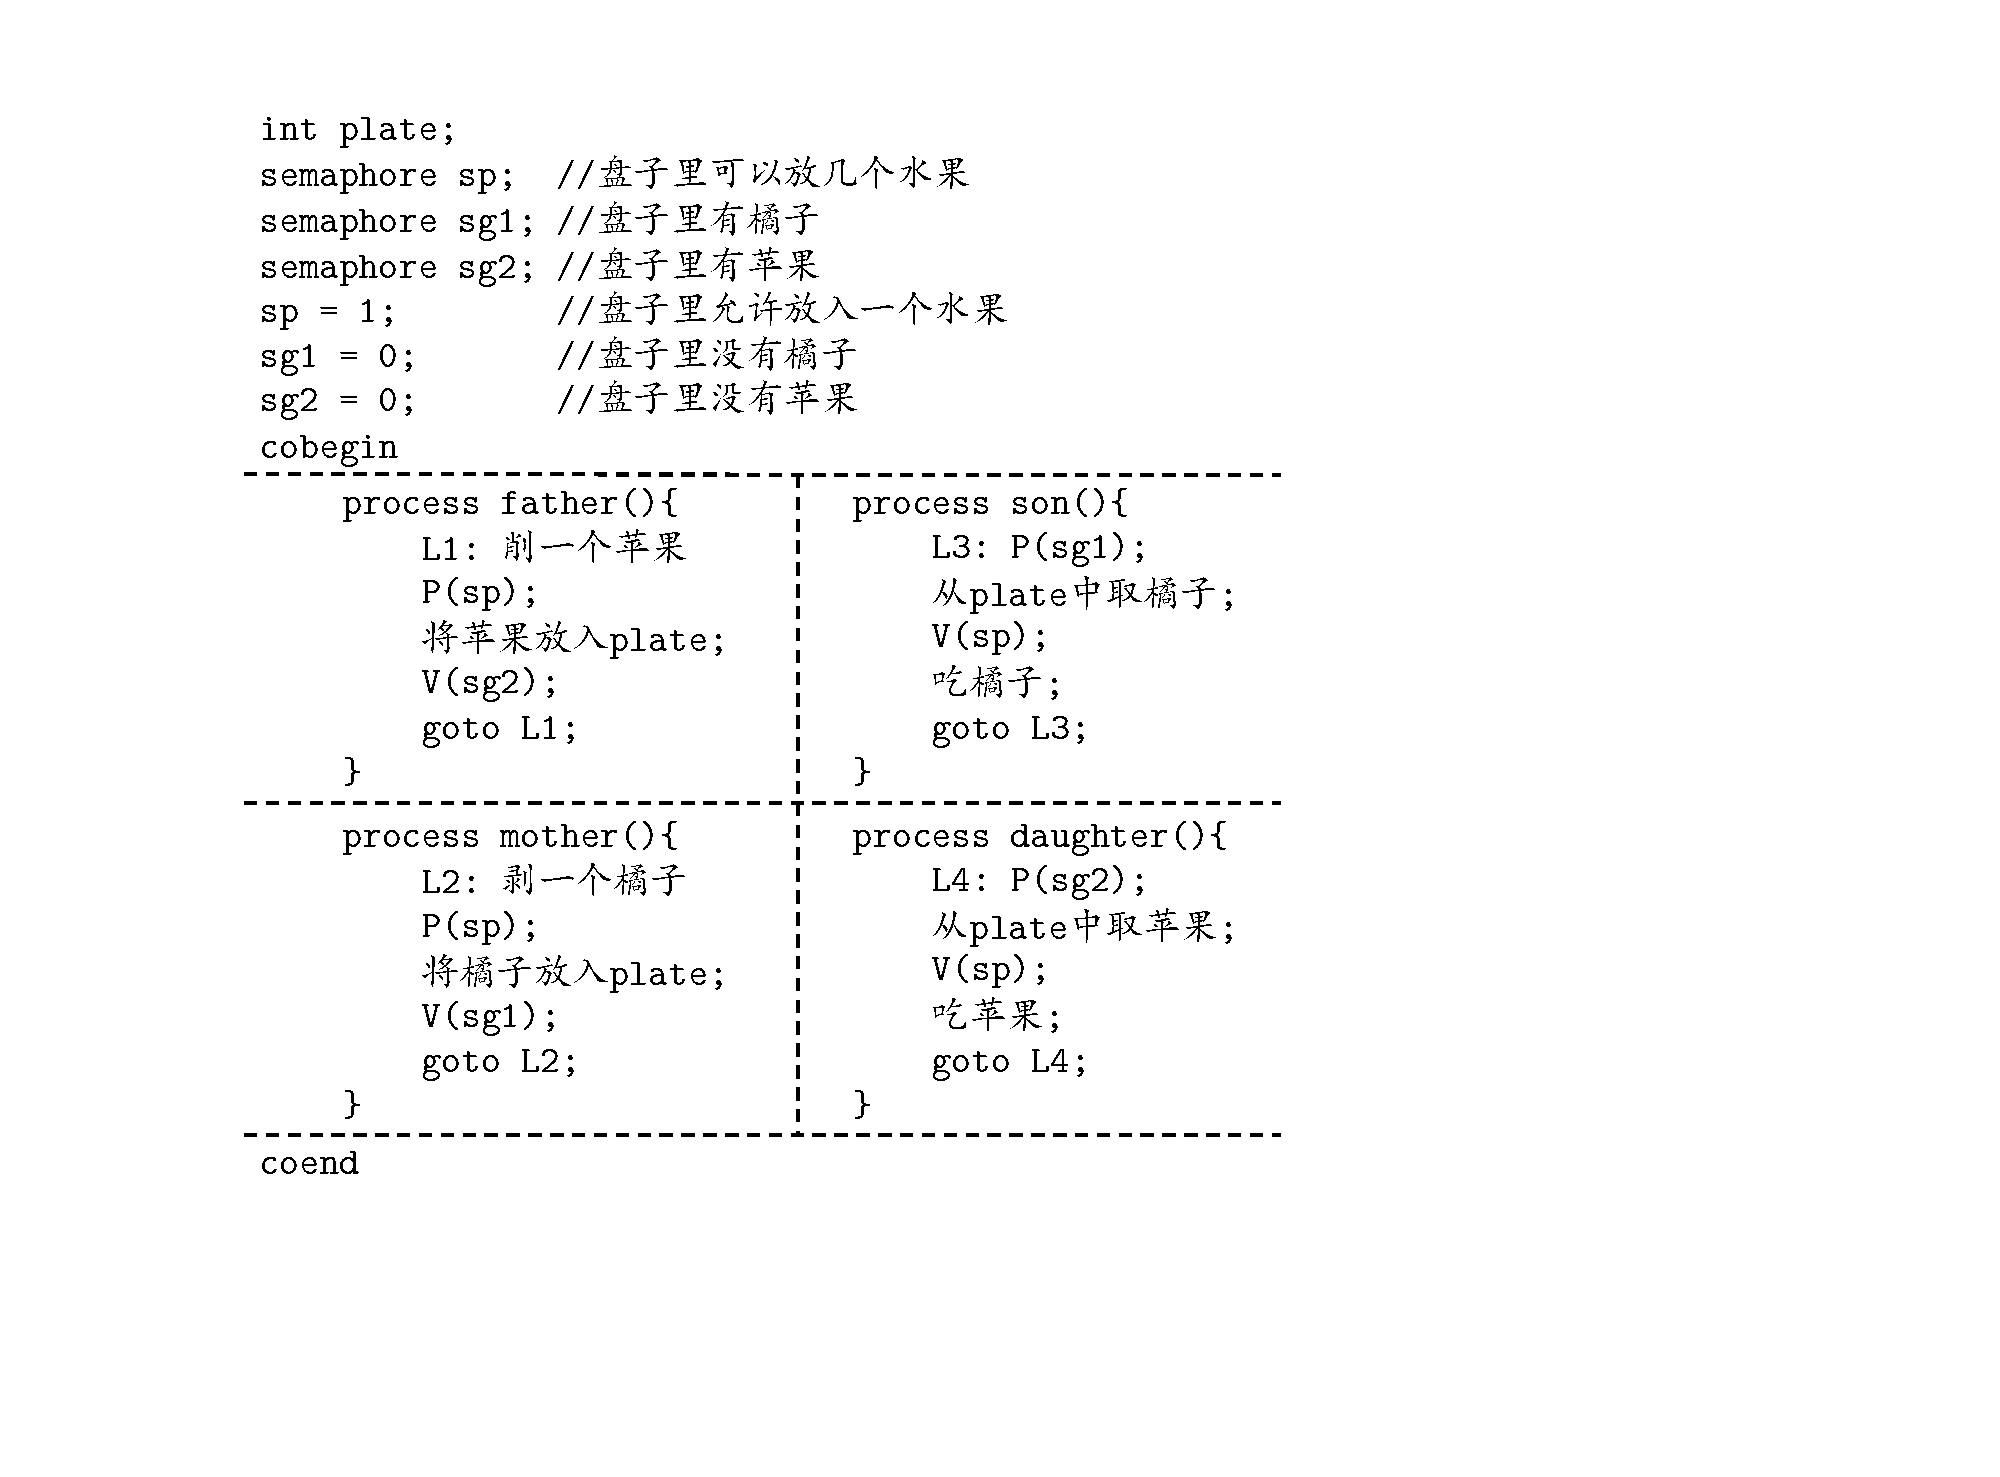
\includegraphics[width=0.65\textwidth]{img/苹果-橘子问题.pdf}
	\end{figure}

	\section{信号量与PV操作习题}

	\subsection{读者/写者问题}
	读者与写者问题(Courtois, 1971):有两组并发进程:读者和写者,共享一个文件$F$,要求:
	\begin{enumerate}[label=\arabic*.]
		\item 允许多个读者可同时对文件执行读操作
		\item 只允许一个写者往文件中写信息
		\item 任意写者在完成写操作之前不允许其他读者或写者工作
		\item 写者执行写操作前,应让已有的写者和读者全部退出
	\end{enumerate}

	\subsubsection{读者优先}
	\begin{lstlisting}[language=C, keywordstyle=\color{black}]
semaphore rmutex, wmutex;
rmutex = 1; wmutex = 1;
int readcount = 0;			//读进程计数
	
process reader_i(){
	while(true){
		P(rmutex);	//上锁进行读者计数更新,防止多个读者计数发生计数冲突的问题
			readcount++;	
			if(readcount == 1)	P(wmutex);	//如果自己是第一个读者,则对文件上锁
		V(rmutex);	//开锁允许其他读者			
		读文件;
		P(rmutex);	//上锁进行读者计数更新,防止多个读者计数发生计数冲突的问题
			readcount--;	//因为已经完成读操作,所以读者计数减1
			if(readcount == 0)	V(wmutex); //如果自己是最后一个读者,则释放文件资源
		V(rmutex);
	}
}

process writer_i(){
	while(true){
		P(wmutex);			//文件上锁
			写文件;
		V(wmutex);			//开锁允许其他进程的读或写操作
	}
}
	\end{lstlisting}
	该程序的设计思路是第一个读者对文件执行占用,最后一个读者对文件执行释放。也正是由于最后一个读者才会释放文件资源,所以当有写者的时候,写者会被阻塞直到所有的读者完成操作。因此这种解法的问题是可能会饿死写者,该解法是读者优先的。

	\subsubsection{写者优先}
	\begin{lstlisting}[language=C, keywordstyle=\color{black}]
int readcount = 0, writecount = 0;
semaphore x = 1, y = 1, z = 1;
semaphore rmutex = 1, wmutex = 1;

process reader_i(){
	while(true){
		P(z);
			P(rmutex);
				P(x);
					readcount++;
					if(readcount == 1)	P(wmutex);
				V(x);
			V(rmutex);
		V(z);
		读文件;
		P(x);
			readcount--;
			if (readcount == 0)			V(wmutex);
		V(x);
	}
}

process writer_i(){
	while(true){
		P(y);
			writecount++;
			if(writecount == 1)	P(rmutex);
		V(y);
		P(wmutex);
			写操作;
		V(wmutex);
		P(y);
			writecount--;
			if(writecount == 0)	V(rmutex);
		V(y);
	}
}
	\end{lstlisting}



	\subsubsection{读写平衡}
	\begin{lstlisting}[language=C, keywordstyle=\color{black}]
semaphore rmutex, wmutex, S;
rmutex = 1; wmutex = 1; S = 1;
int readcount = 0;
process reader_i(){
	while(true){
		P(S);
			P(rmutex);
				readcount++;	
				if(readcount == 1)	P(wmutex);	
			V(rmutex);		
		V(S);	
		读文件;
		P(rmutex);	
			readcount--;
			if(readcount == 0)		V(wmutex);
		V(rmutex);
	}
}

process writer_i(){
	while(true){
		P(S);
			P(wmutex);
				写文件;
			V(wmutex);
		V(S);
	}
}
	\end{lstlisting}


	\verb|S|\ 一次对外面提供一个服务的空位,不管是读者还是写者都需要先抢占这个空位

	\subsection{睡眠的理发师问题}
	问题描述:理发店理有一位理发师、一把理发椅和$n$把供等候理发的顾客坐的椅子
	\begin{itemize}
		\item 如果没有顾客,理发师便在理发椅上睡觉
		\item 一个顾客到来时,它必须叫醒理发师
		\item 如果理发师正在理发时又有顾客来到,则如果有空椅子可坐,就坐下来等待,否则就离开
	\end{itemize}

	\begin{figure}[H]
		\centering
		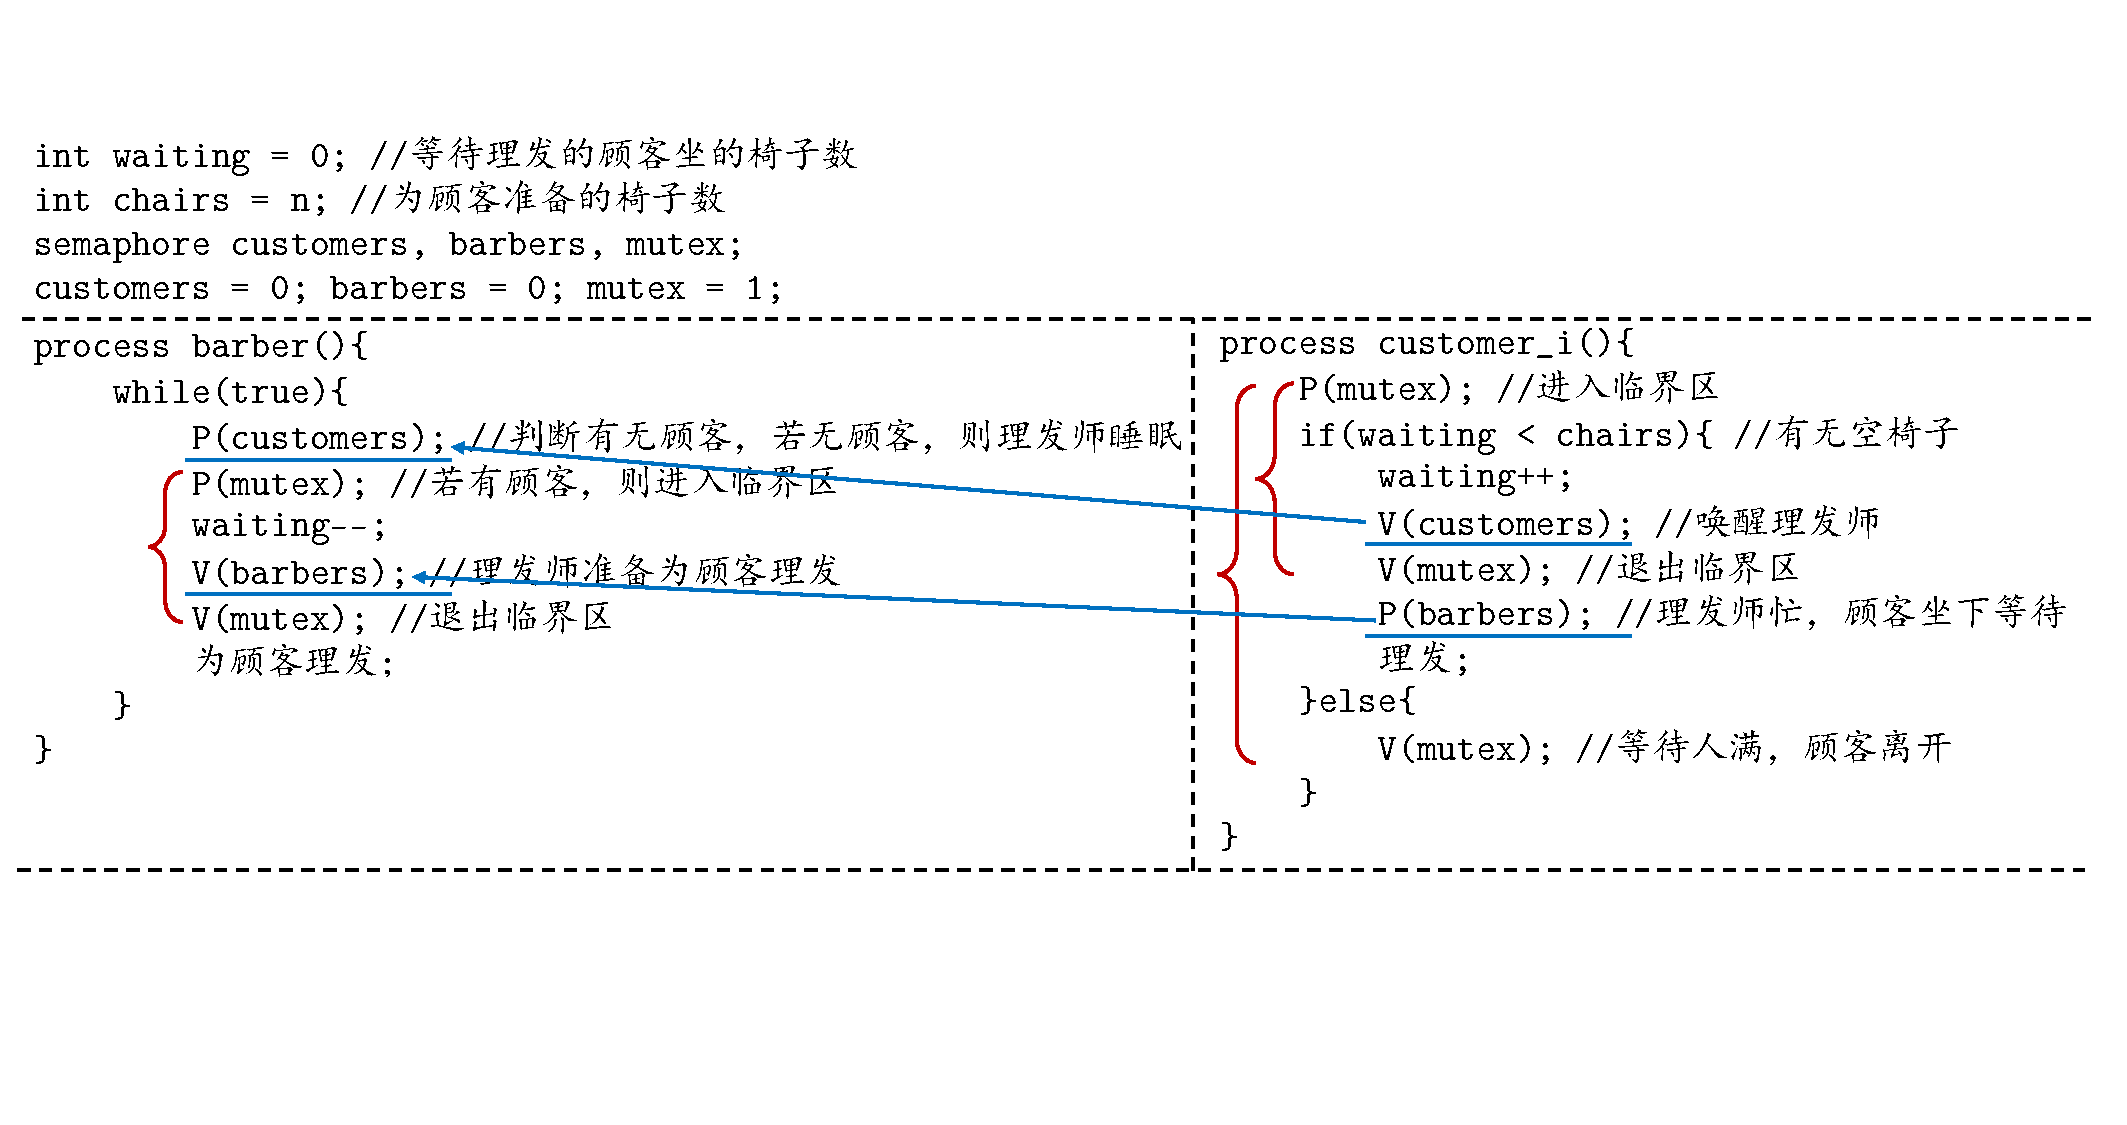
\includegraphics[width=0.98\textwidth]{img/理发师问题.pdf}
	\end{figure}

	\subsection{农夫猎人问题}
	问题描述:有一个铁笼子,每次只能放入一个动物。猎手向笼中放入老虎,农夫向笼中放入羊,动物园等待取笼中的老虎,饭店等待取笼中的羊。

	\begin{figure}[H]
		\centering
		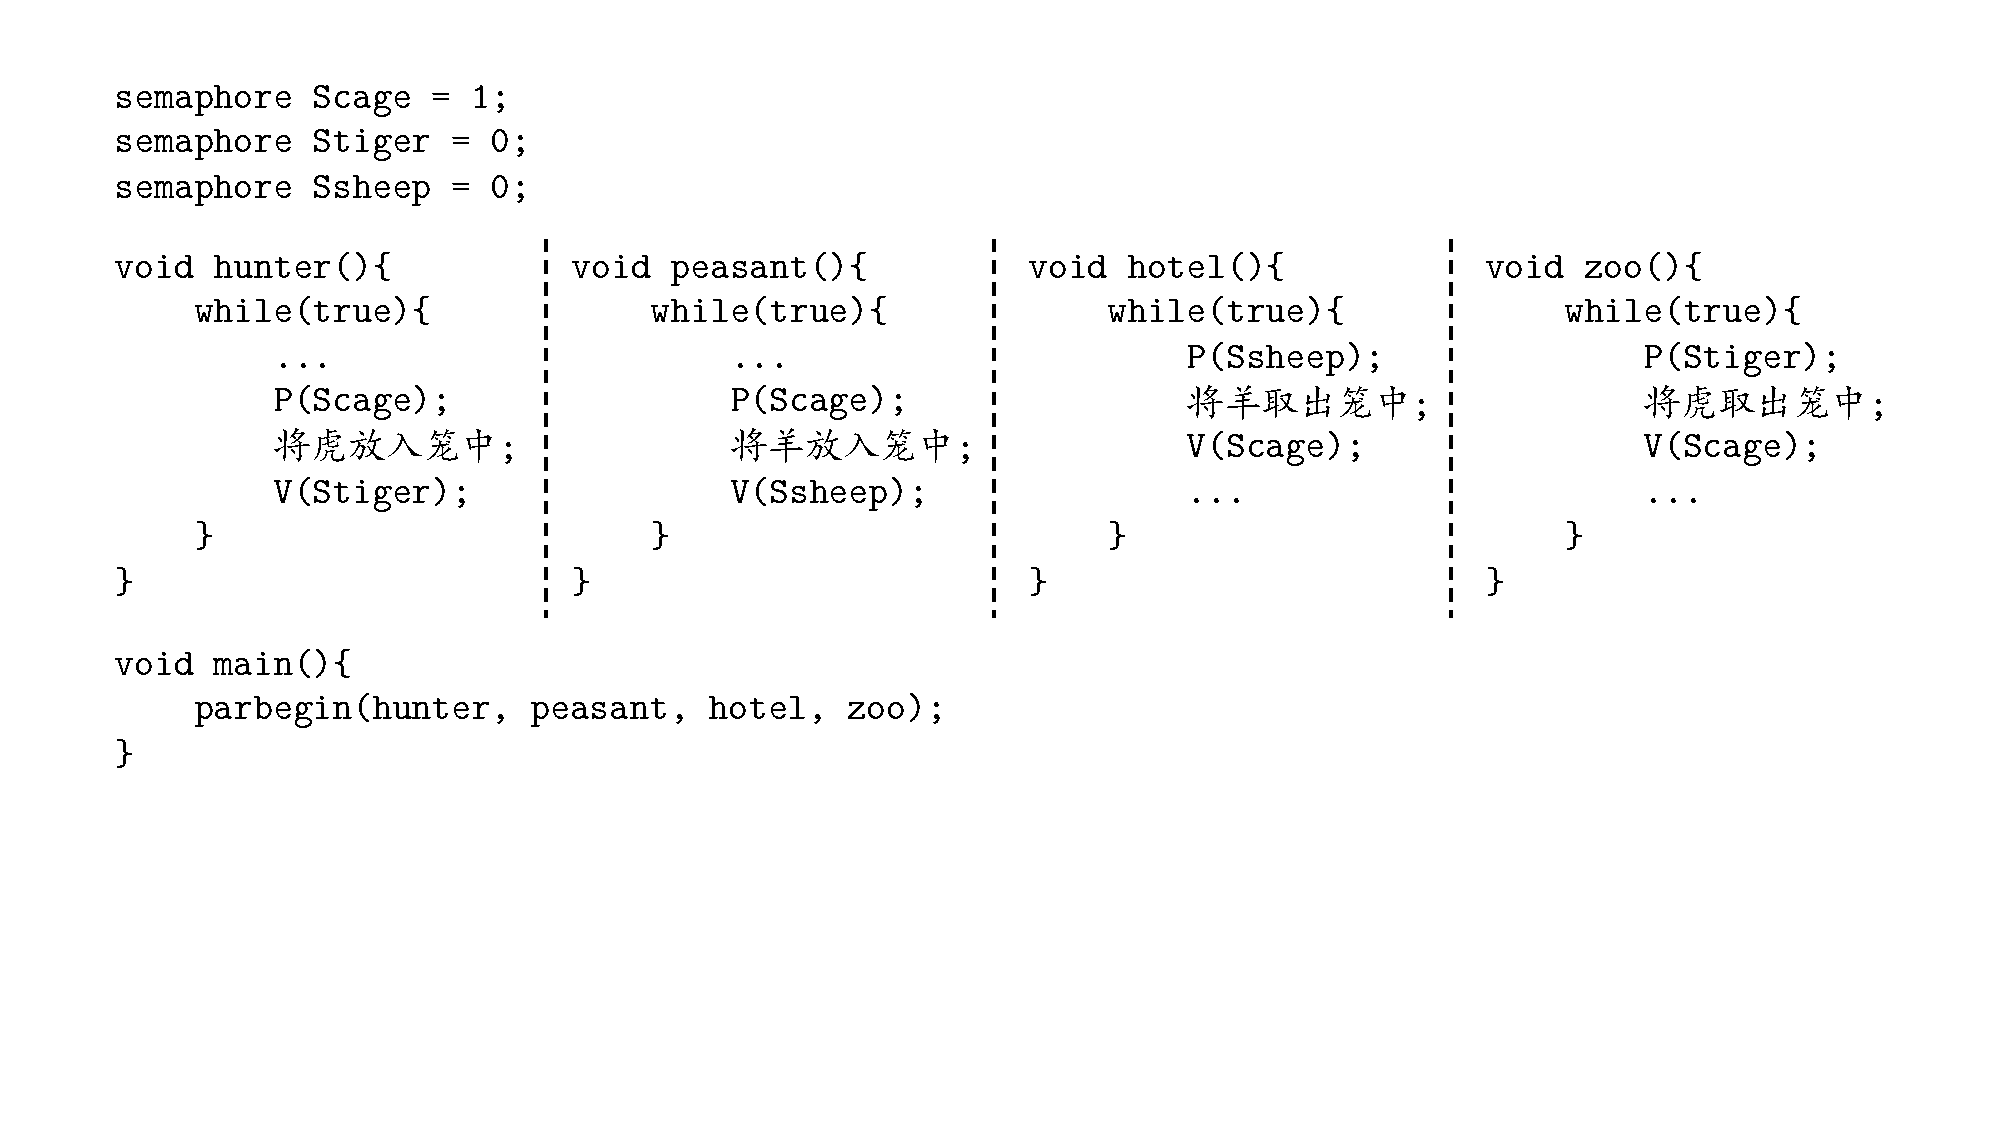
\includegraphics[width=0.98\textwidth]{img/农夫猎人问题.pdf}
	\end{figure}

	\subsection{银行业务问题}
	问题描述:某大型银行办理人民币储蓄业务,由$n$个储蓄员负责。每个顾客进入银行后先至取号机取一个号,并且在等待区找到空沙发坐下等着叫号。取号机给出的号码依次递增,并假定有足够多的空沙发容纳顾客。当一个储蓄员空闲下来,就叫下一个号。

	\begin{figure}[H]
		\centering
		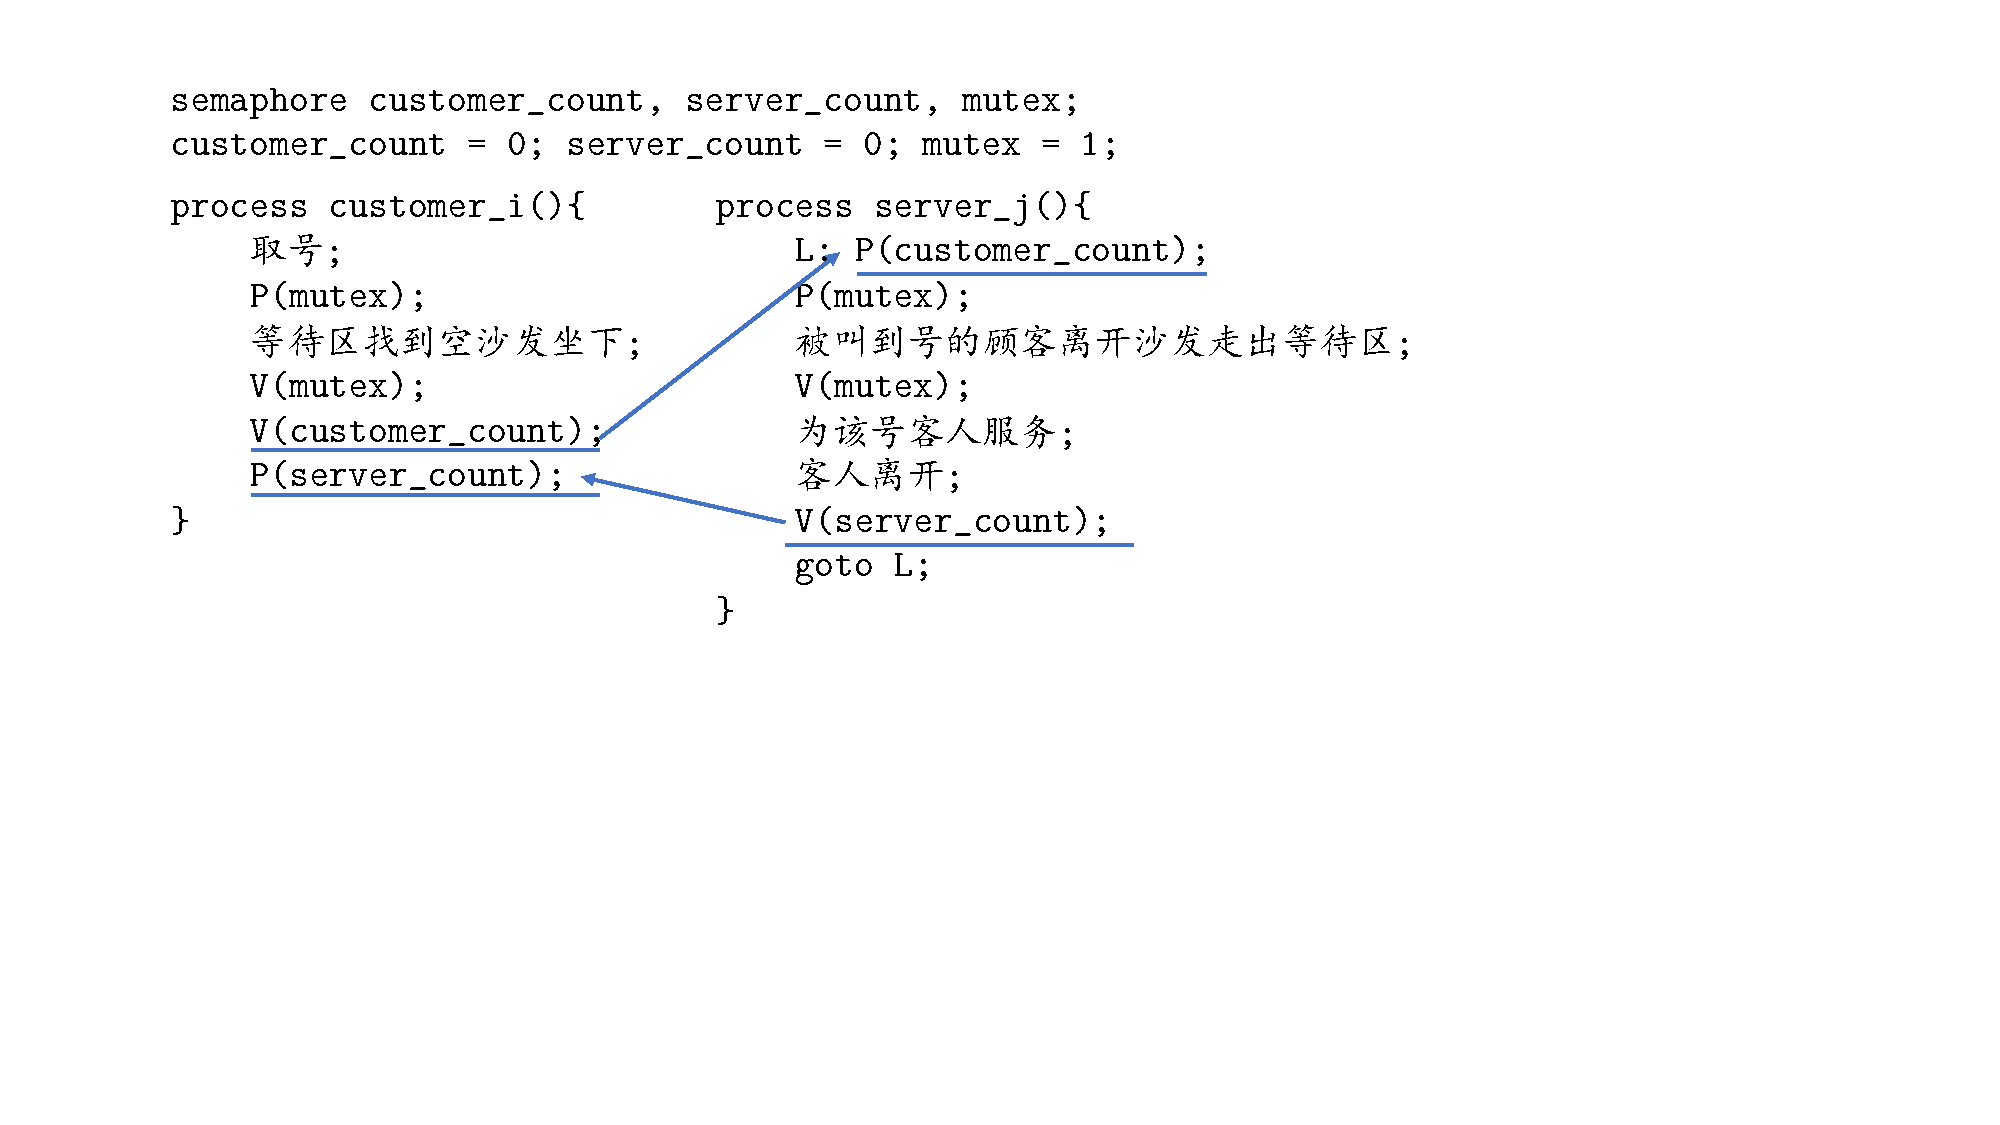
\includegraphics[width=0.75\textwidth]{img/银行业务问题.pdf}
	\end{figure}

	\subsection{缓冲区管理}
	问题描述:有$n$个进程将字符逐个读入到一个容量为80的缓冲区中($n>1$),当缓冲区满后,由输出进程$Q$负责一次性取走这80个字符,这种过程循环往复。

	\begin{figure}[H]
		\centering
		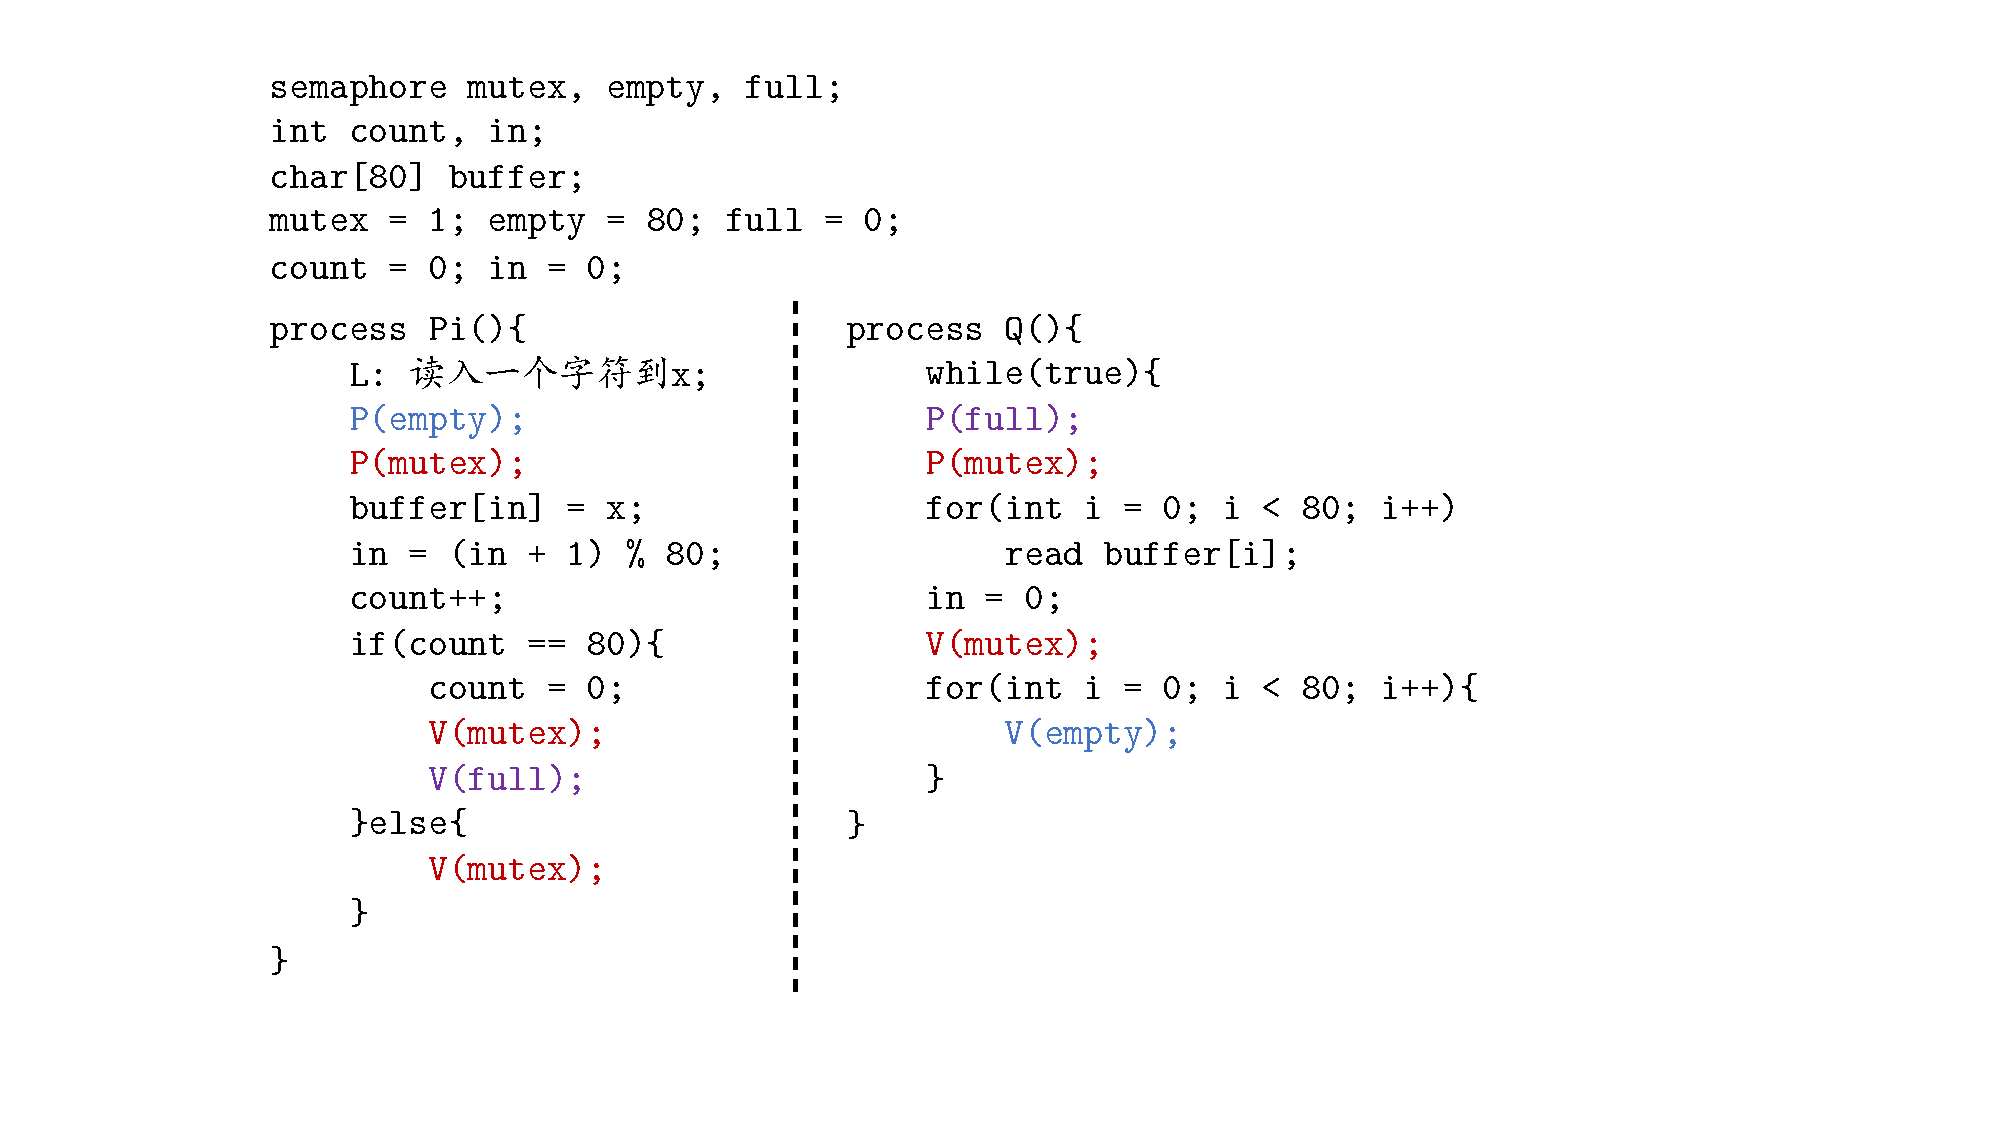
\includegraphics[width=0.8\textwidth]{img/缓冲区管理.pdf}
	\end{figure}

	\subsection{售票问题}
	问题描述:汽车司机与售票员之间必须协同工作,一方面只有售票员把车门关好了司机才能开车,因此,售票员 关好门应通知司机开车,然后售票员进行售票。另一方面,只有当汽车已经停下,售票员才能开门上下客,故司机停车后应该通知售票员。
	
	现假定某辆公共汽车上有一名司机与两名售票员,汽车当前正在始发站停车上客。

	\begin{figure}[H]
		\centering
		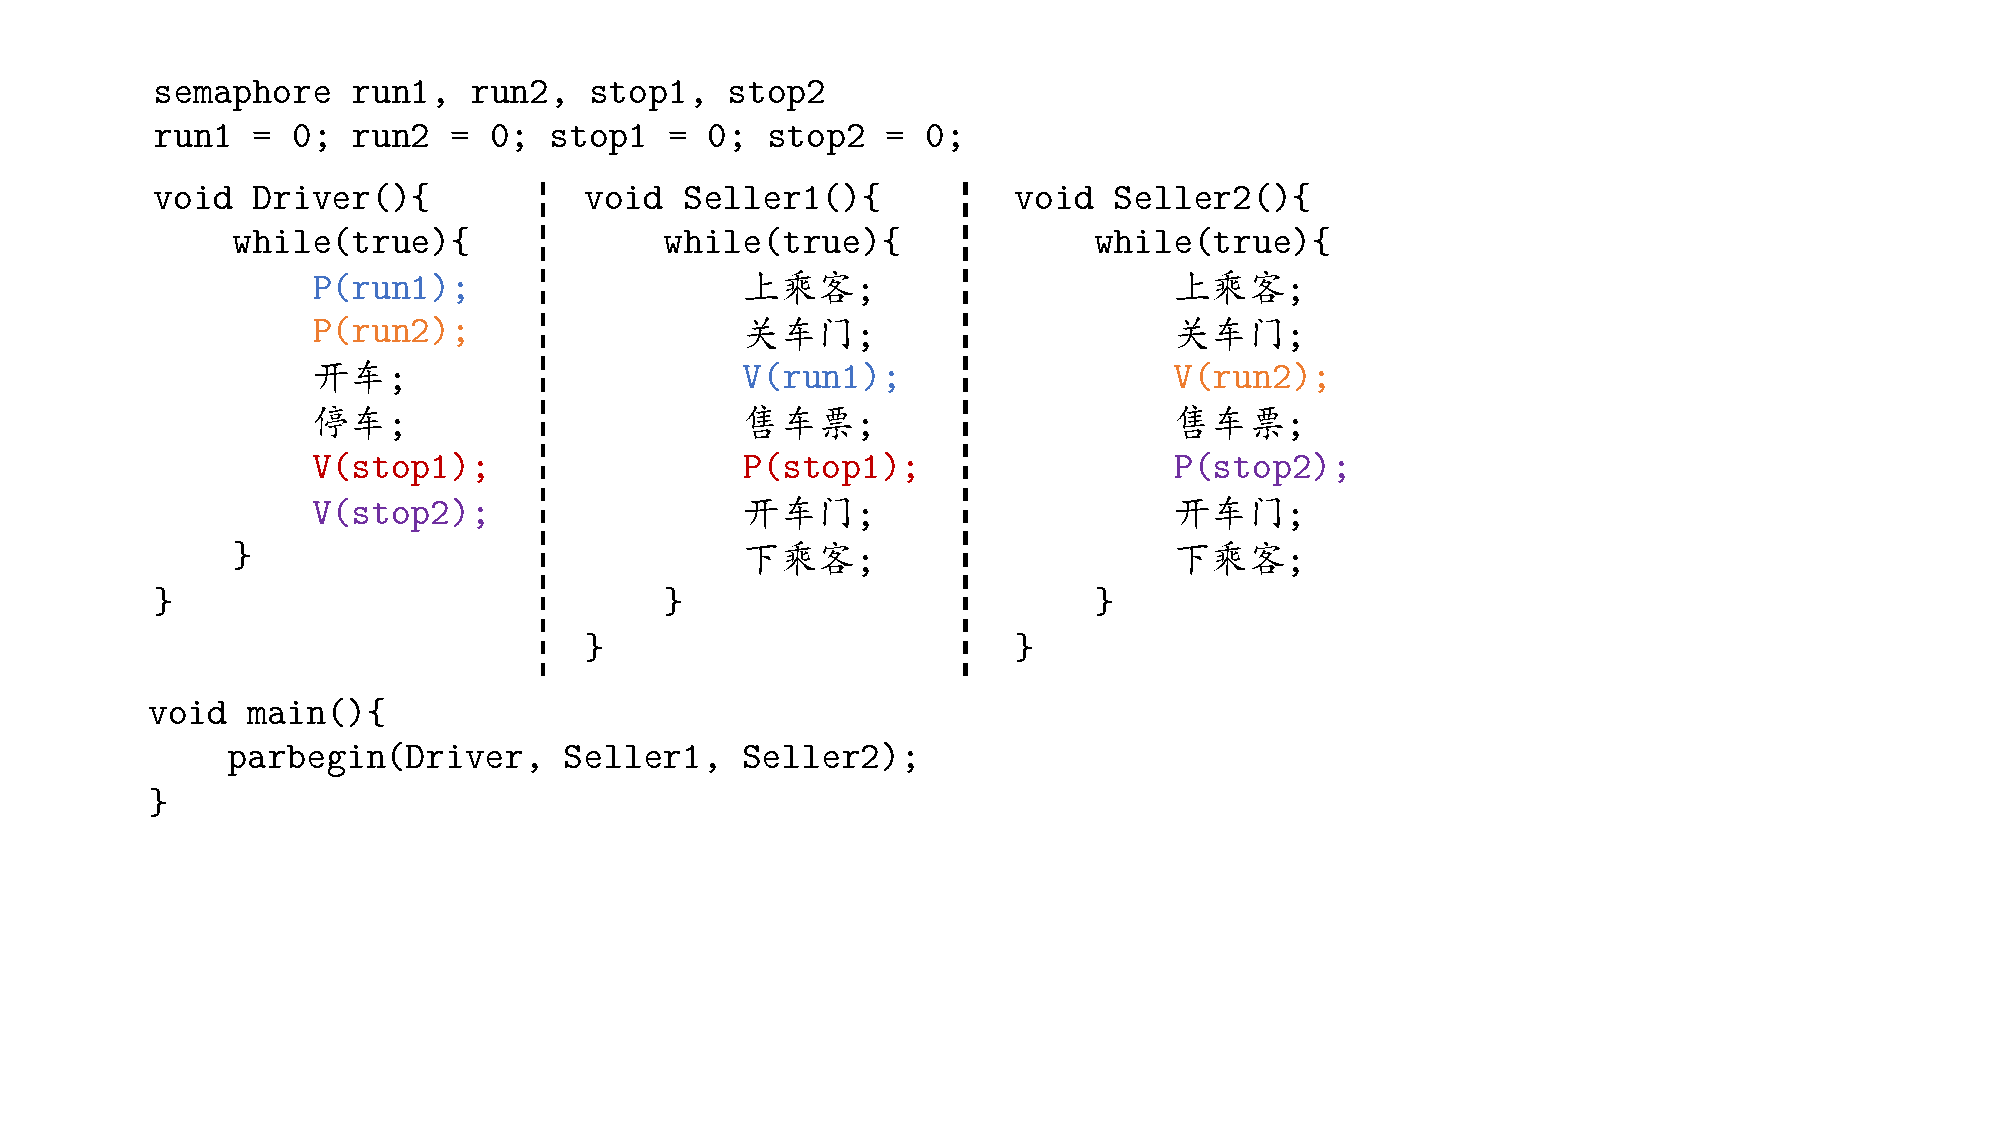
\includegraphics[width=0.75\textwidth]{img/售票问题.pdf}
	\end{figure}

	\subsection{吸烟者问题}
	问题描述:三个吸烟者在一个房间内,还有一个香烟供应者。为了制造并抽掉香烟,每个吸烟者需要三样东西:烟草、纸和火柴,供应者有丰富货物提供。三个吸烟者中,第一个有自己的烟草,第二个有自己的纸和第三个有自己的火柴。供应者随机地将两样东西放在桌子上,允许一个吸烟者进行对健康不利的吸烟。当吸烟者完成吸烟后唤醒供应者,供应者再把两样东西放在桌子上,唤醒另一个吸烟者。

	\begin{figure}[H]
		\centering
		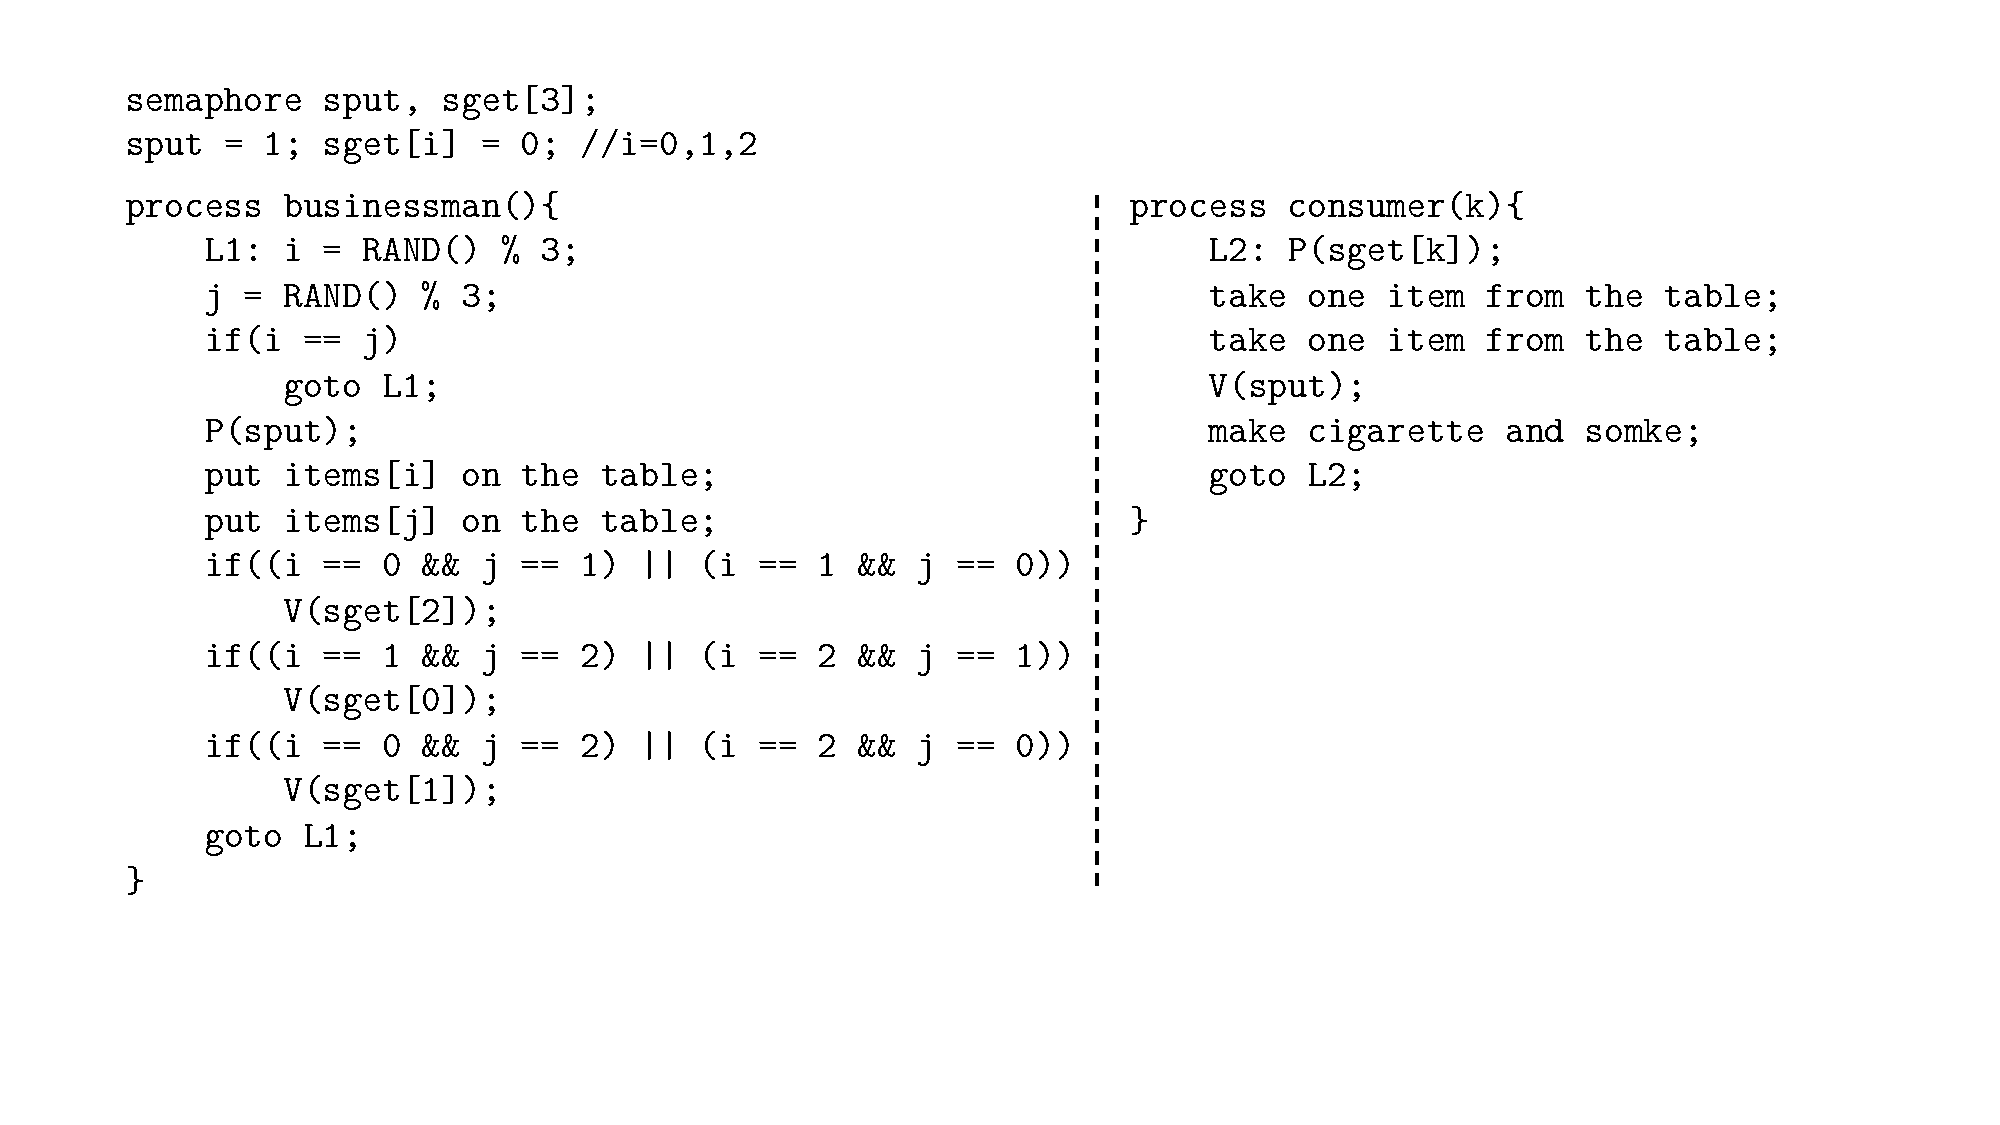
\includegraphics[width=0.9\textwidth]{img/吸烟者问题.pdf}
	\end{figure}

	\subsection{独木桥问题}
	\subsubsection{独木桥问题1}
	问题描述:东西向汽车过独木桥,为了保证安全,只要桥上无车,则允许一方的汽车过桥,待一方的车全部过完后,另一方的车才允许过桥。

	\begin{figure}[H]
		\centering
		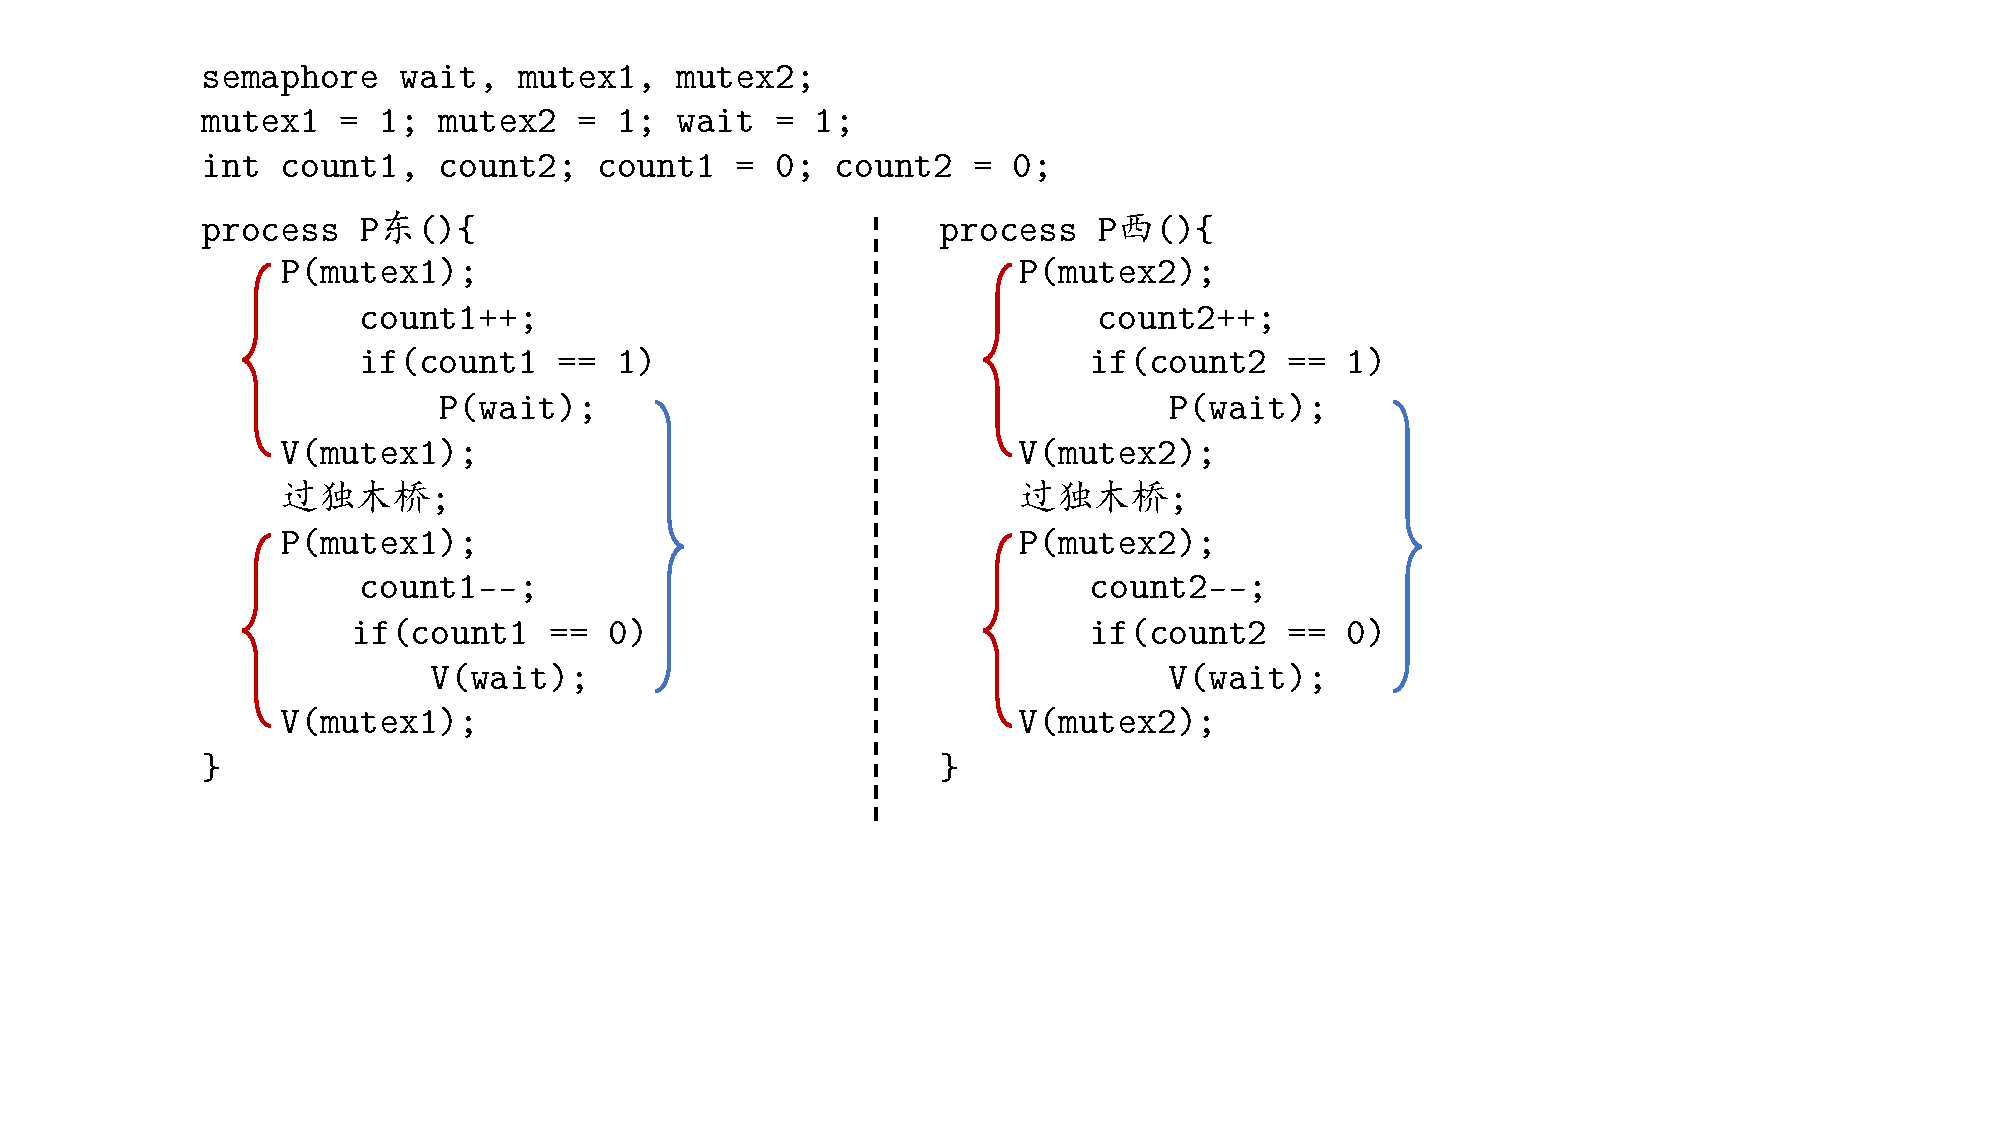
\includegraphics[width=0.65\textwidth]{img/独木桥问题1.pdf}
	\end{figure}				

	
	\subsubsection{独木桥问题2}
	问题描述:在独木桥问题1的基础上,限制桥面上最多可以有$k$辆汽车通过。

	\begin{figure}[H]
		\centering
		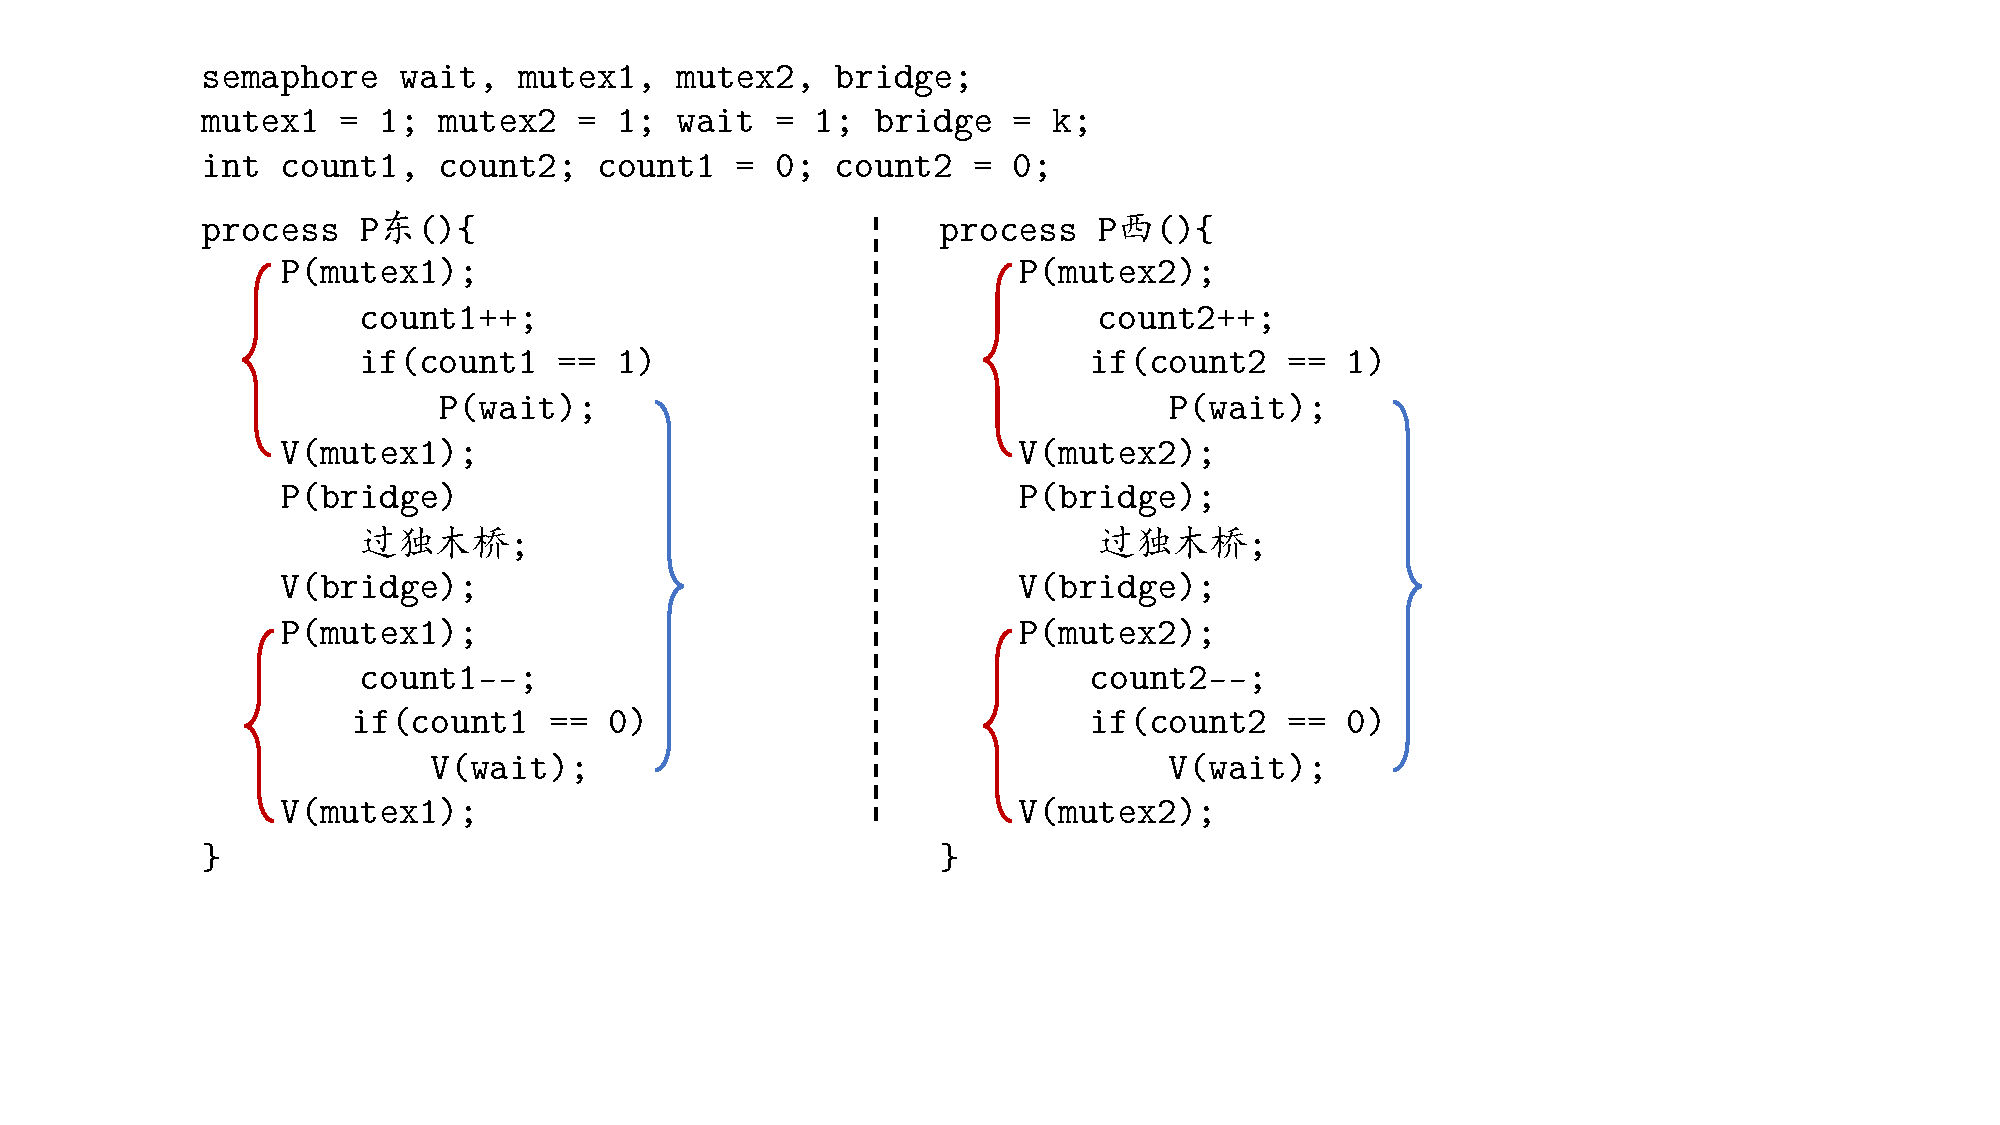
\includegraphics[width=0.7\textwidth]{img/独木桥问题2.pdf}
	\end{figure}


	\subsubsection{独木桥问题3}
	问题描述:在独木桥问题1的基础上,以3辆汽车为一组,要求保证东方和西方以组为单位交替通过汽车。

	\begin{figure}[H]
		\centering
		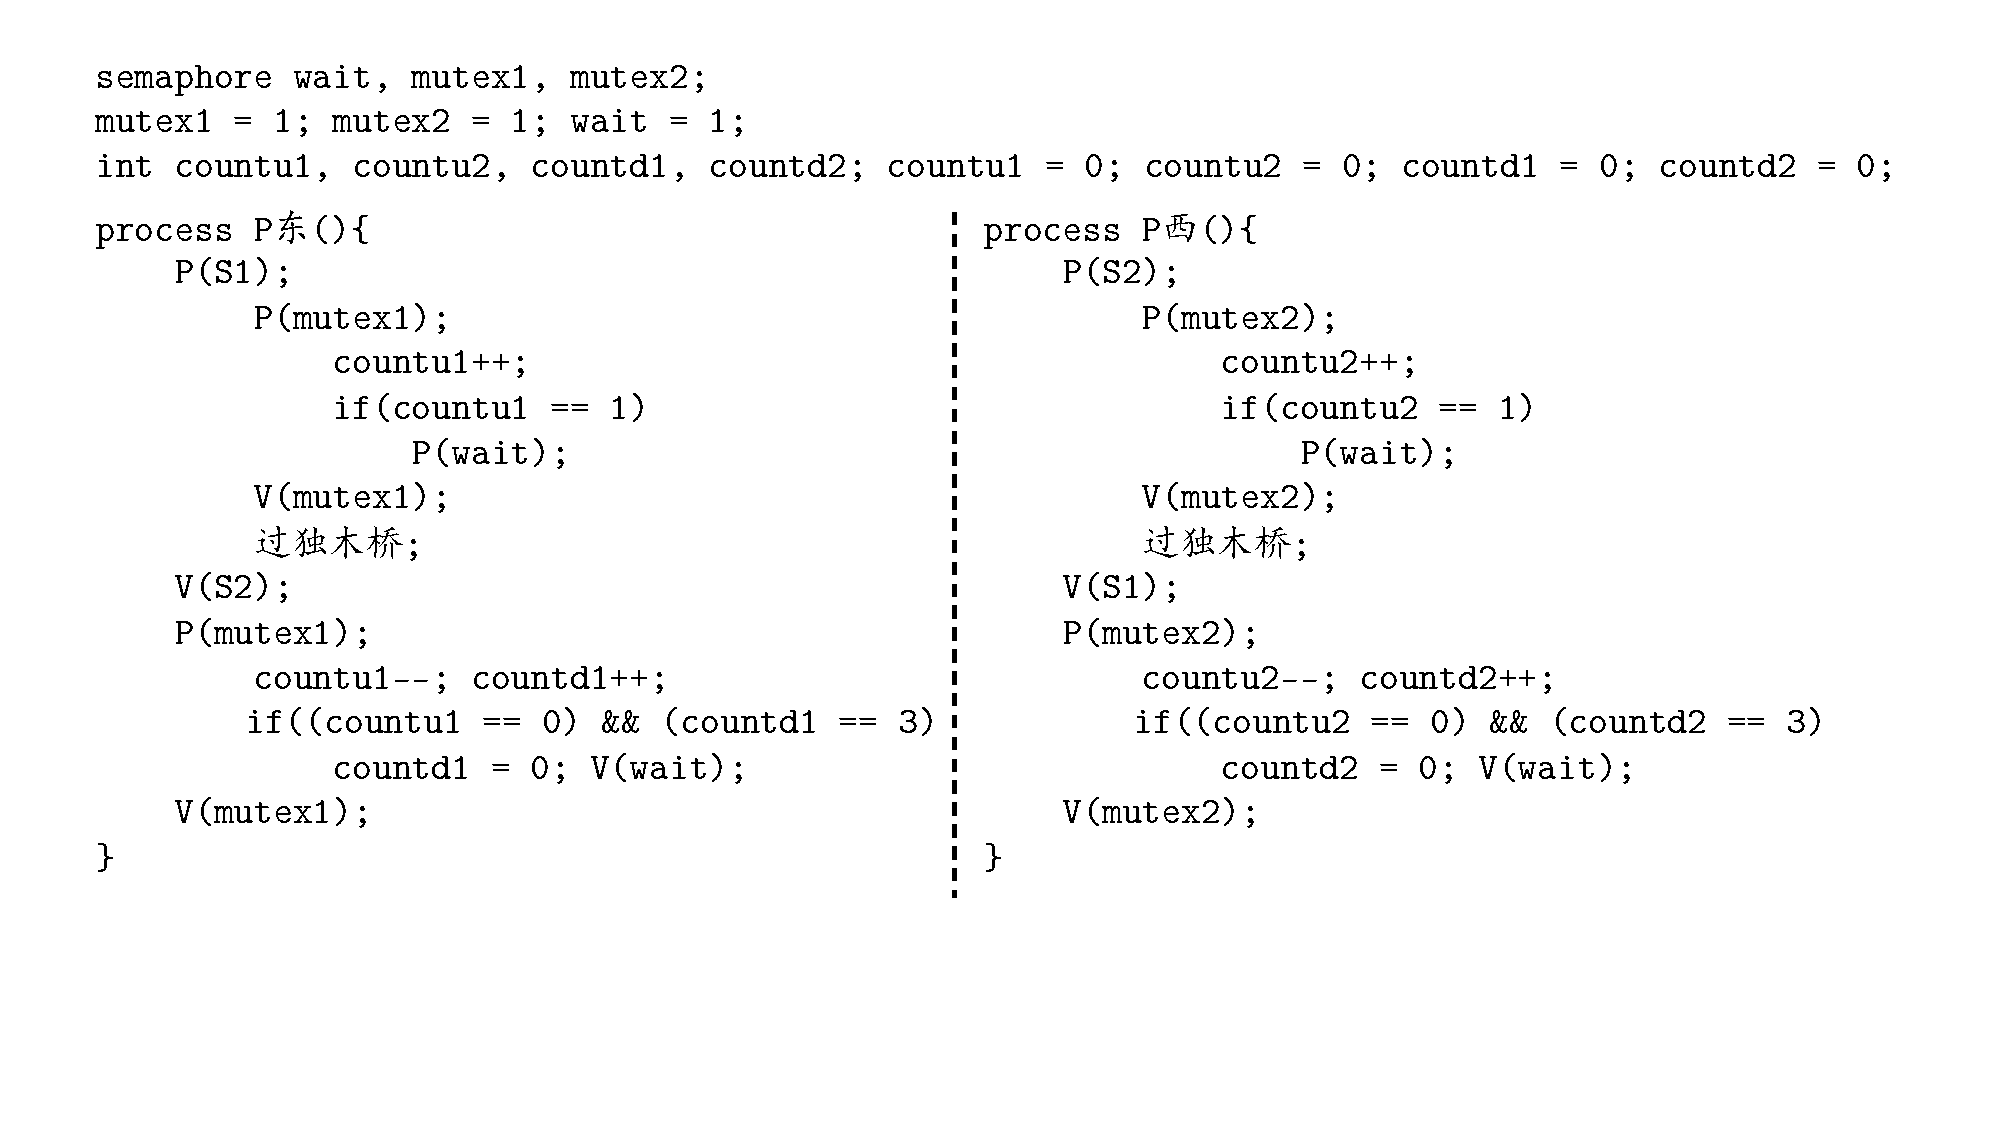
\includegraphics[width=0.98\textwidth]{img/独木桥问题3.pdf}
	\end{figure}


	\subsubsection{独木桥问题4}
	问题描述:在独木桥问题1的基础上,要求各方向的汽车串行过桥,但当另一方提出过桥时,应能阻止对方未上桥的后继车辆,待桥面上的汽车过完桥后,另一方的汽车开始过桥。

	\begin{figure}[H]
		\centering
		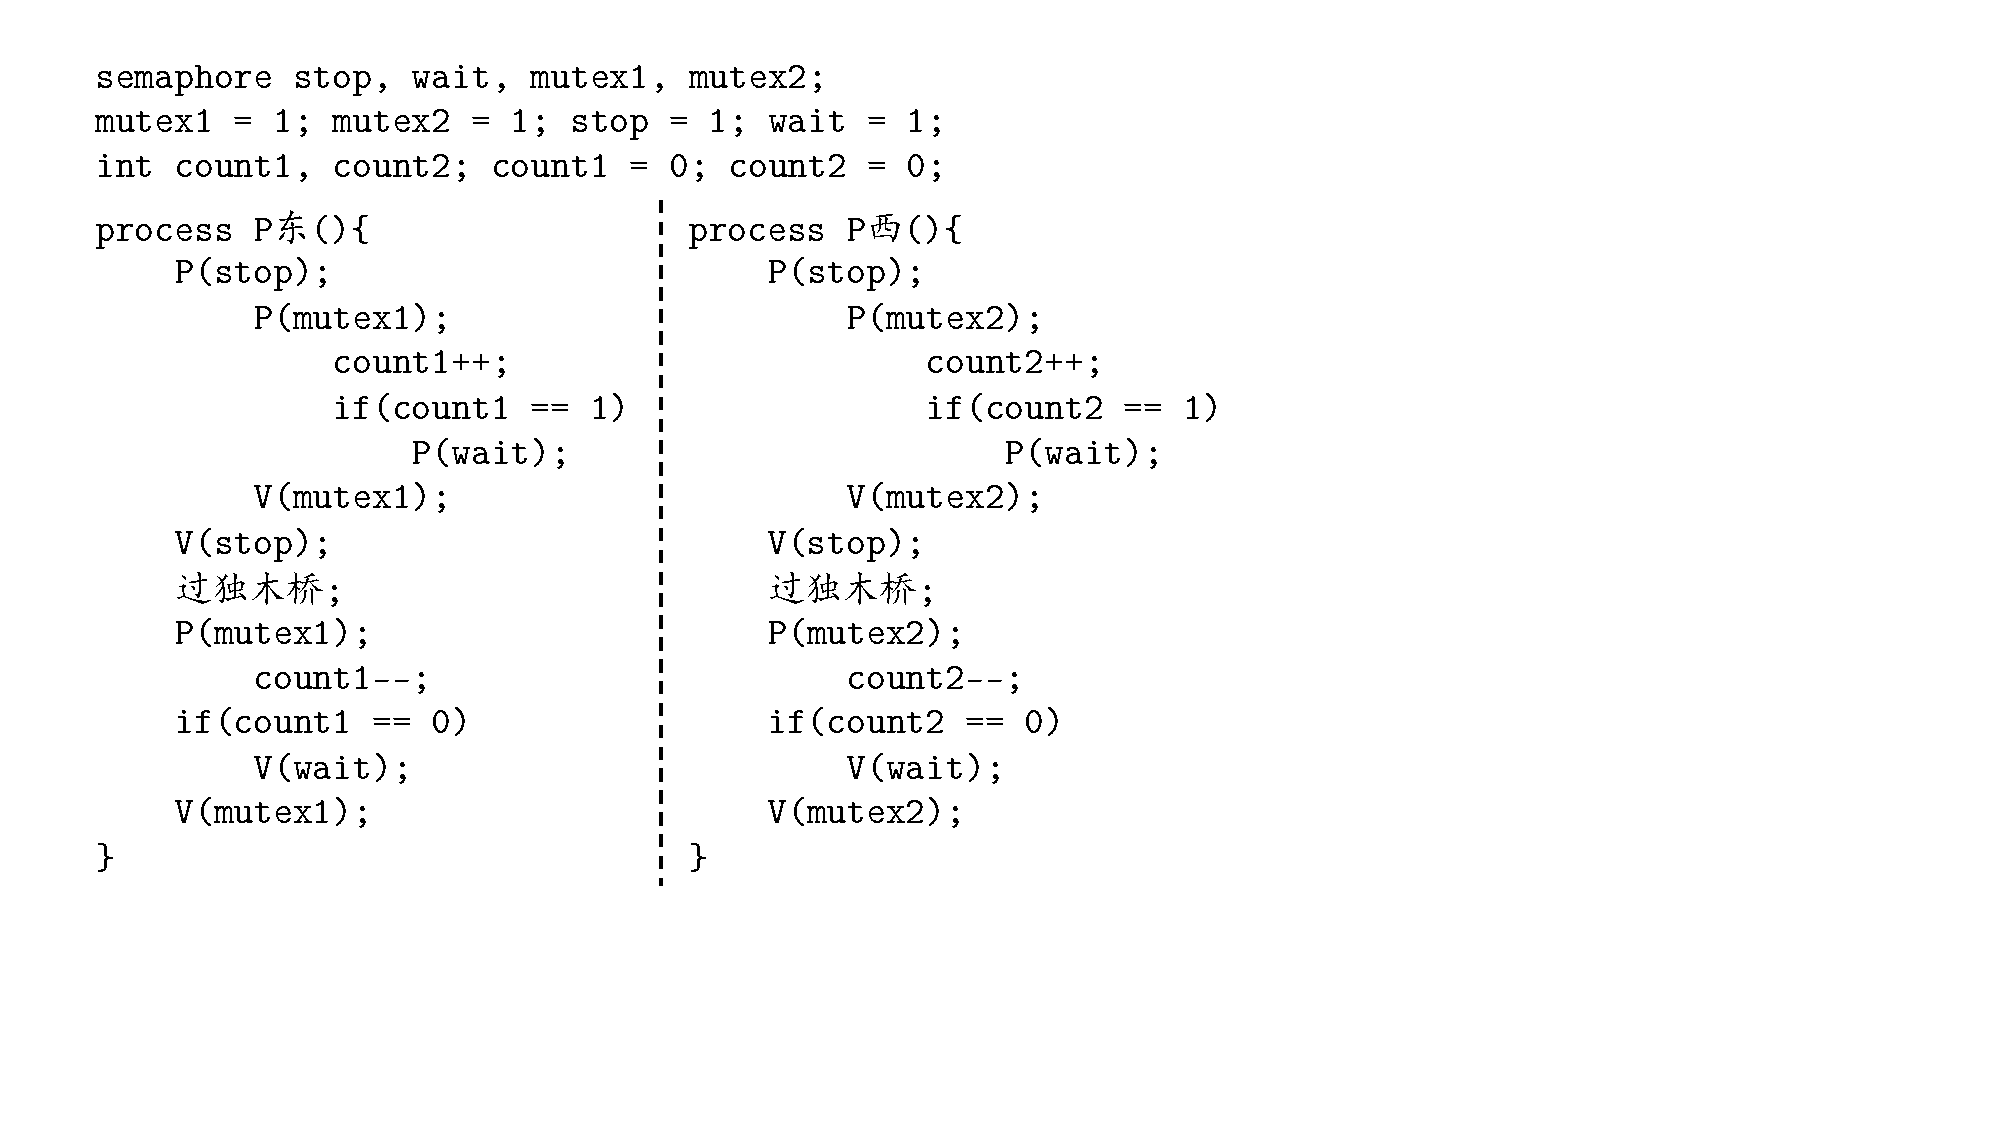
\includegraphics[width=0.7\textwidth]{img/独木桥问题4.pdf}
	\end{figure}


	\section{管程}
	\subsection{管程概述}

	\subsubsection{管程的提出}
	管程是由若干公共变量及其说明和所有访问这些变量的过程所组成
	\begin{itemize}
		\item 管程把分散在各个进程中互斥地访问公共变量的那些临界区集中起来管理
		\item 管程的局部变量只能由该管程的过程存取
	\end{itemize}

	管程的属性:
	\begin{enumerate}[label=\arabic*.]
		\item 共享性:管程中的移出过程可被所有调用管程的过程的进程所共享
		\item 安全性:管程的局部变量只能由此管程内部分访问,不允许进程或其他管程直接访问
		\item 互斥性:任一时刻,共享资源的进程可以访问管程中的管理此资源的过程,但最多只有一个调用者能够真正进入管程,其他调用者必须等待直到管程可用
	\end{enumerate}

	\subsubsection{管程的规格定义与实现思路}
	每个管程都有一个名字以供标识,其一般形式为:
	\begin{lstlisting}[language=C, keywordstyle=\color{black}]
type <管程名> = monitor {
	局部变量说明;
	条件变量说明;
	初始化语句;
	define <(能被其他模块引用的)过程名列表>;
	use <(要引用的模块外定义的)过程名列表>;
	procedure <过程名>(<形式参数表>);

	过程名/函数名(形式参数表) {
		<过程/函数体>;
	}
	
	...
   
   过程名/函数名(形式参数表) {
      <过程/函数体>;
   }
}
	\end{lstlisting}

	管程的执行模型:
	\begin{figure}[H]
		\centering
		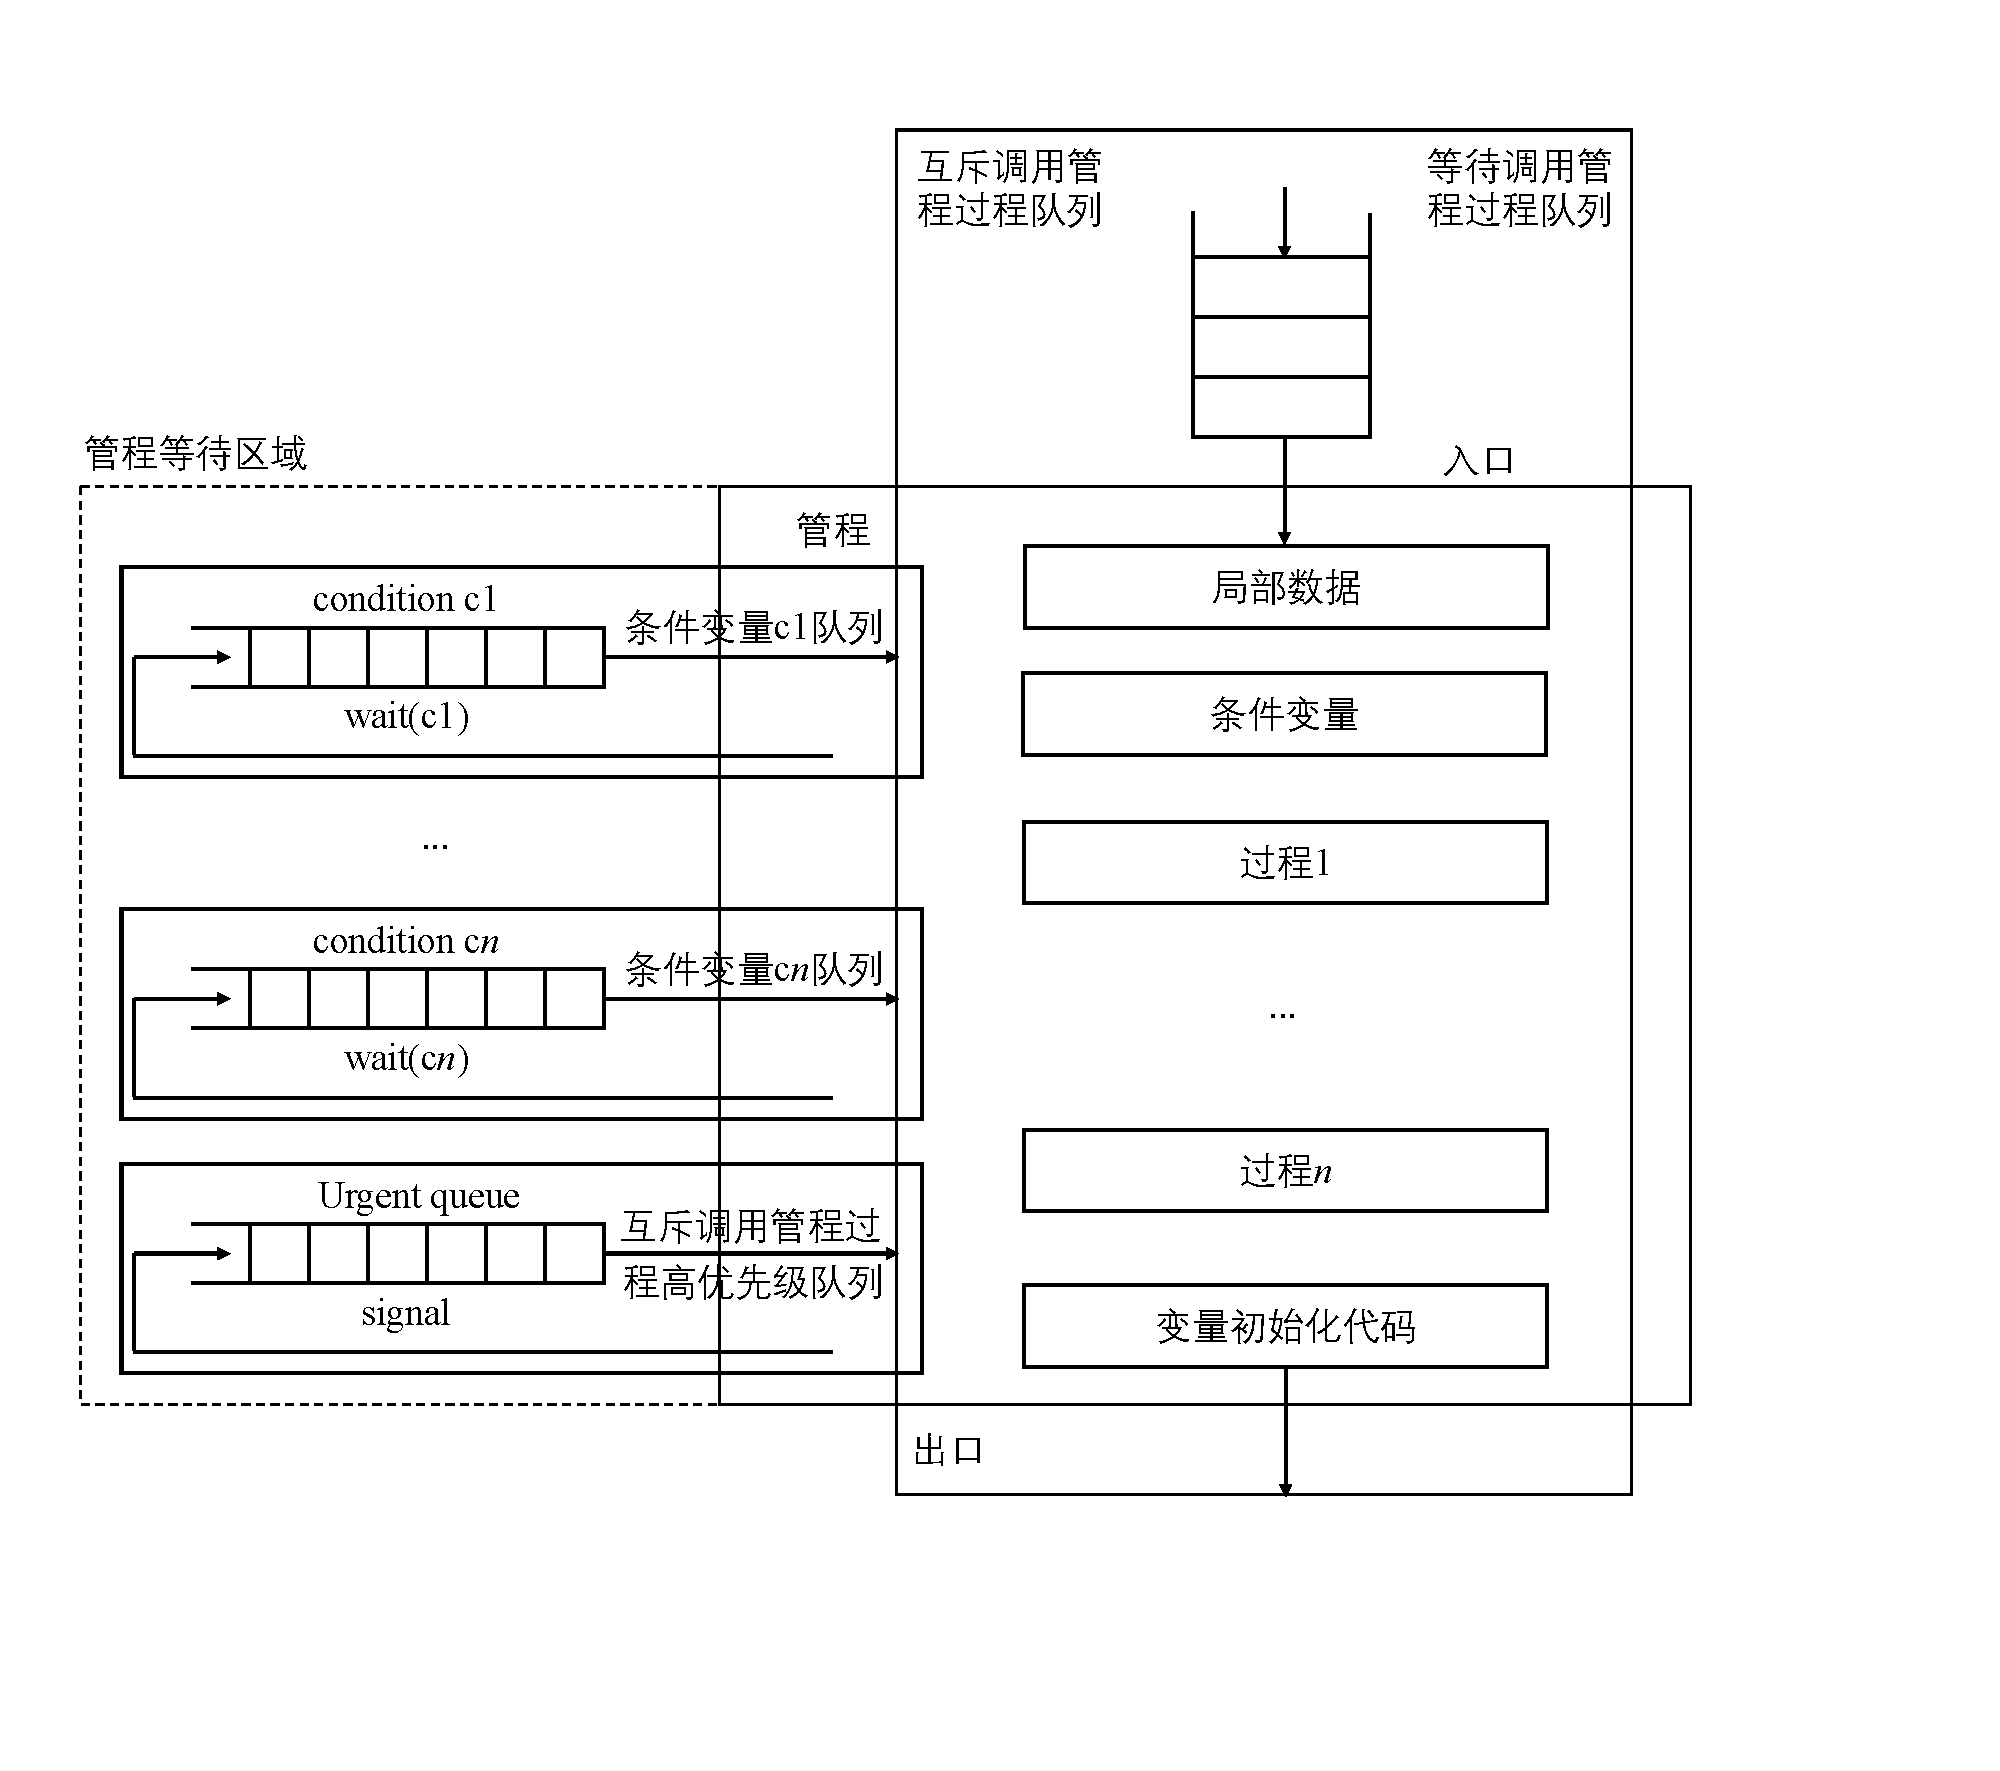
\includegraphics[width=0.75\textwidth]{img/管程的执行模型.pdf}
	\end{figure}
	条件变量是出现在管程内的一种数据结构,且只有在管程中才能被访问,它对管程内的所有过程是全局的,只能通过两个原语操作来控制它:
	\begin{itemize}
		\item \verb|wait()|:阻塞调用进程并释放管程,直到另一个进程在该条件变量上执行\ \verb|signal()|
		\item \verb|signal()|:如果存在其他进程由于对条件变量执行\ \verb|wait()|\ 而被阻塞,便释放之;如果没有进程在等待,那么则信号不被保存
	\end{itemize}

	使用\ \verb|signal|\ 释放等待进程时,可能出现两个进程同时停留在管程内,解决方法有:
	\begin{itemize}
		\item 执行\ \verb|signal|\ 的进程等待,直到被释放进程退出管程或等待另一个条件变量
		\begin{itemize}
			\item 霍尔(Hoare)采用该办法
		\end{itemize}
		\item 被释放进程等待,直到执行\ \verb|signal|\ 的进程退出管程 或等待另一个条件
		\begin{itemize}
			\item 汉森(Hansen)选择两者的折衷,规定管程中的过程所执行的\ \verb|signal|\ 操作是过程体的最后一个操作
		\end{itemize}
	\end{itemize}

	管程和进程的对比:
	\begin{itemize}
		\item 管程定义公用数据结构,进程定义私有数据结构
		\item 管程将共享变量上的同步操作集中统一管理,临界区分散在每个进程中
		\item 管程为了解决进程共享资源的互斥,进程为了占有系统资源和实现系统并发
		\item 管程被想要使用共享资源的所有进程调用,管程和调用它的进程不能并行工作;进程间可以并行工作
	\end{itemize}

	\subsection{霍尔管程}
	霍尔管程是一种更具普适性的管程实现方法,它使用PV操作原语实现对管程中过程的互斥调用功能,同时实现对共享资源互斥使用的管理。
	\begin{itemize}
		\item 每当有进程等待资源时,霍尔管程将让执行signal操作的进程阻塞自己,直到它被释放的进程退出管程或产生了其他的等待条件为止
		\item 与汉森管程的实现方法相比,该方法不要求signal操作是过程体的最后一个操作,且wait和signal操作可被设计成两个可以中断的过程,而非原语
		\item 霍尔管程可以通过操作系统的程序库或高级程序设计语言,在基础操作系统的PV操作原语上实现,而不需要扩展操作系统的内核
	\end{itemize}

	\subsubsection{霍尔管程的数据结构}
	\begin{lstlisting}[language=C,keywordstyle=\color{black}]
typedef struct InterfaceModule{ //InterfaceModule是结构体名字
	semaphore mutex; 	//进程调用管程过程前使用的互斥信号量
	semaphore next; 	//发出signal的进程阻塞自己的信号量
	int next_count; 	//在next上等待的进程数
};
mutex=1; next=0; next_count=0;	//初始化语句
	\end{lstlisting}

	\begin{itemize}
		\item \verb|mutex|
		\begin{itemize}
			\item 对每个管程,使用用于管程中过程互斥调用的信号量\verb|mutex|(初值为1)
			\item 进程调用管程中的任何过程时,应执行\verb|P(mutex)|;进程退出管程时,需要判断是否有进程在next信号量等待,如果有(即\verb|next-count>0|),则通过\verb|V(next)|唤醒一个发出\verb|signal|的进程,否则应执行\verb|V(mutex)|开放管程,以便让其他调用者进入
			\item 为了使进程在等待资源期间,其他进程能进入管程,故在\verb|wait|操作中也必须执行\verb|V(mutex)|,否则会妨碍其他进程进入管程,导致无法释放资源
		\end{itemize}
		\item \verb|next|和\verb|next-count|
		\begin{itemize}
			\item 对每个管程,引入信号量\verb|next|(初值为0),凡发出\verb|signal|操作的进程应该用\verb|P(next)|阻塞自己,直到被释放进程退出管程或产生其他等待条件
			\item 进程在退出管程的过程前,须检查是否有别的进程 在信号量\verb|next|上等待,若有,则用\verb|V(next)|唤醒它。
			\item \verb|next-count|(初值为0),用来记录在\verb|next|上等待的进程个数
		\end{itemize}
		\item \verb|x-sem|和\verb|x-count|
		\begin{itemize}
			\item 引入信号量\verb|x-sem|(初值为0),申请资源得不到满足时,执行\verb|P(x-sem)|阻塞。由于释放资源时,需要知道是否有别的进程在等待资源,用计数器\verb|x-count|(初值为0)记录等待资源的进程数
			\item 执行\verb|signal|操作时,应让等待资源的诸进程中的某个进程立即恢复运行,而不让其他进程抢先进入管程,这可以用\verb|V(x-sem)|来实现
		\end{itemize}
	\end{itemize}

	\subsubsection{霍尔管程的enter()和leave()操作}
	\begin{lstlisting}[language=C, keywordstyle=\color{black}]
void enter(InterfaceModule &IM) {
	P(IM.mutex);         //判断是否有发出过signal的进程
}

void leave(InterfaceModule &IM) {
	if(IM.next_count > 0)
		V(IM.next);      //有就释放一个发出过signal的进程
	else
		V(IM.mutex);     //否则开放管程
}
	\end{lstlisting}


	\subsubsection{霍尔管程的wait()操作}
	\begin{lstlisting}[language=C, keywordstyle=\color{black}]
void wait(semaphore &x_sem, int &x_count, InterfaceModule &IM) {
	x_count++; 				//等资源进程个数加1,x_count初始化为0
	if (IM.next_count > 0) 	//判断是否有发出过signal的进程
		V(IM.next); 		//有就释放一个 
	else
		V(IM.mutex); 		//否则开放管程
	P(x_sem); 				//等资源进程阻塞自己,x_sem初始化为0 
	x_count--; 				//等资源进程个数减1
}
	\end{lstlisting}

	\subsubsection{霍尔管程的signal()操作}
	\begin{lstlisting}[language=C, keywordstyle=\color{black}]
void signal(semaphore &x_sem, int &x_count, InterfaceModule &IM) {
	if(x_count > 0){ 		//判断是否有等待资源的进程
		IM.next_count++; 	//发出signal进程个数加1 
		V(x_sem); 			//释放一个等资源的进程 
		P(IM.next); 		//发出signal进程阻塞自己 
		IM.next_count--; 	//发出signal进程个数减1
	} 
}
	\end{lstlisting}


	\subsection{霍尔管程求解进程互斥与同步问题}

	\subsubsection{霍尔管程求解读者/写者问题}
	\begin{lstlisting}[language=C, keywordstyle=\color{black}]
tyoe read-write = monitor
	int rc, wc;
	semaphore R, W; R = 0; W = 0; 
	int R_count, W_count;
	rc = 0; wc = 0;
	InterfaceModule IM;
	DEFINE start_read, end_read, start_write, end_write;
	USE wait, signal, enter, leave;
	\end{lstlisting}

	\begin{figure}[H]
		\centering
		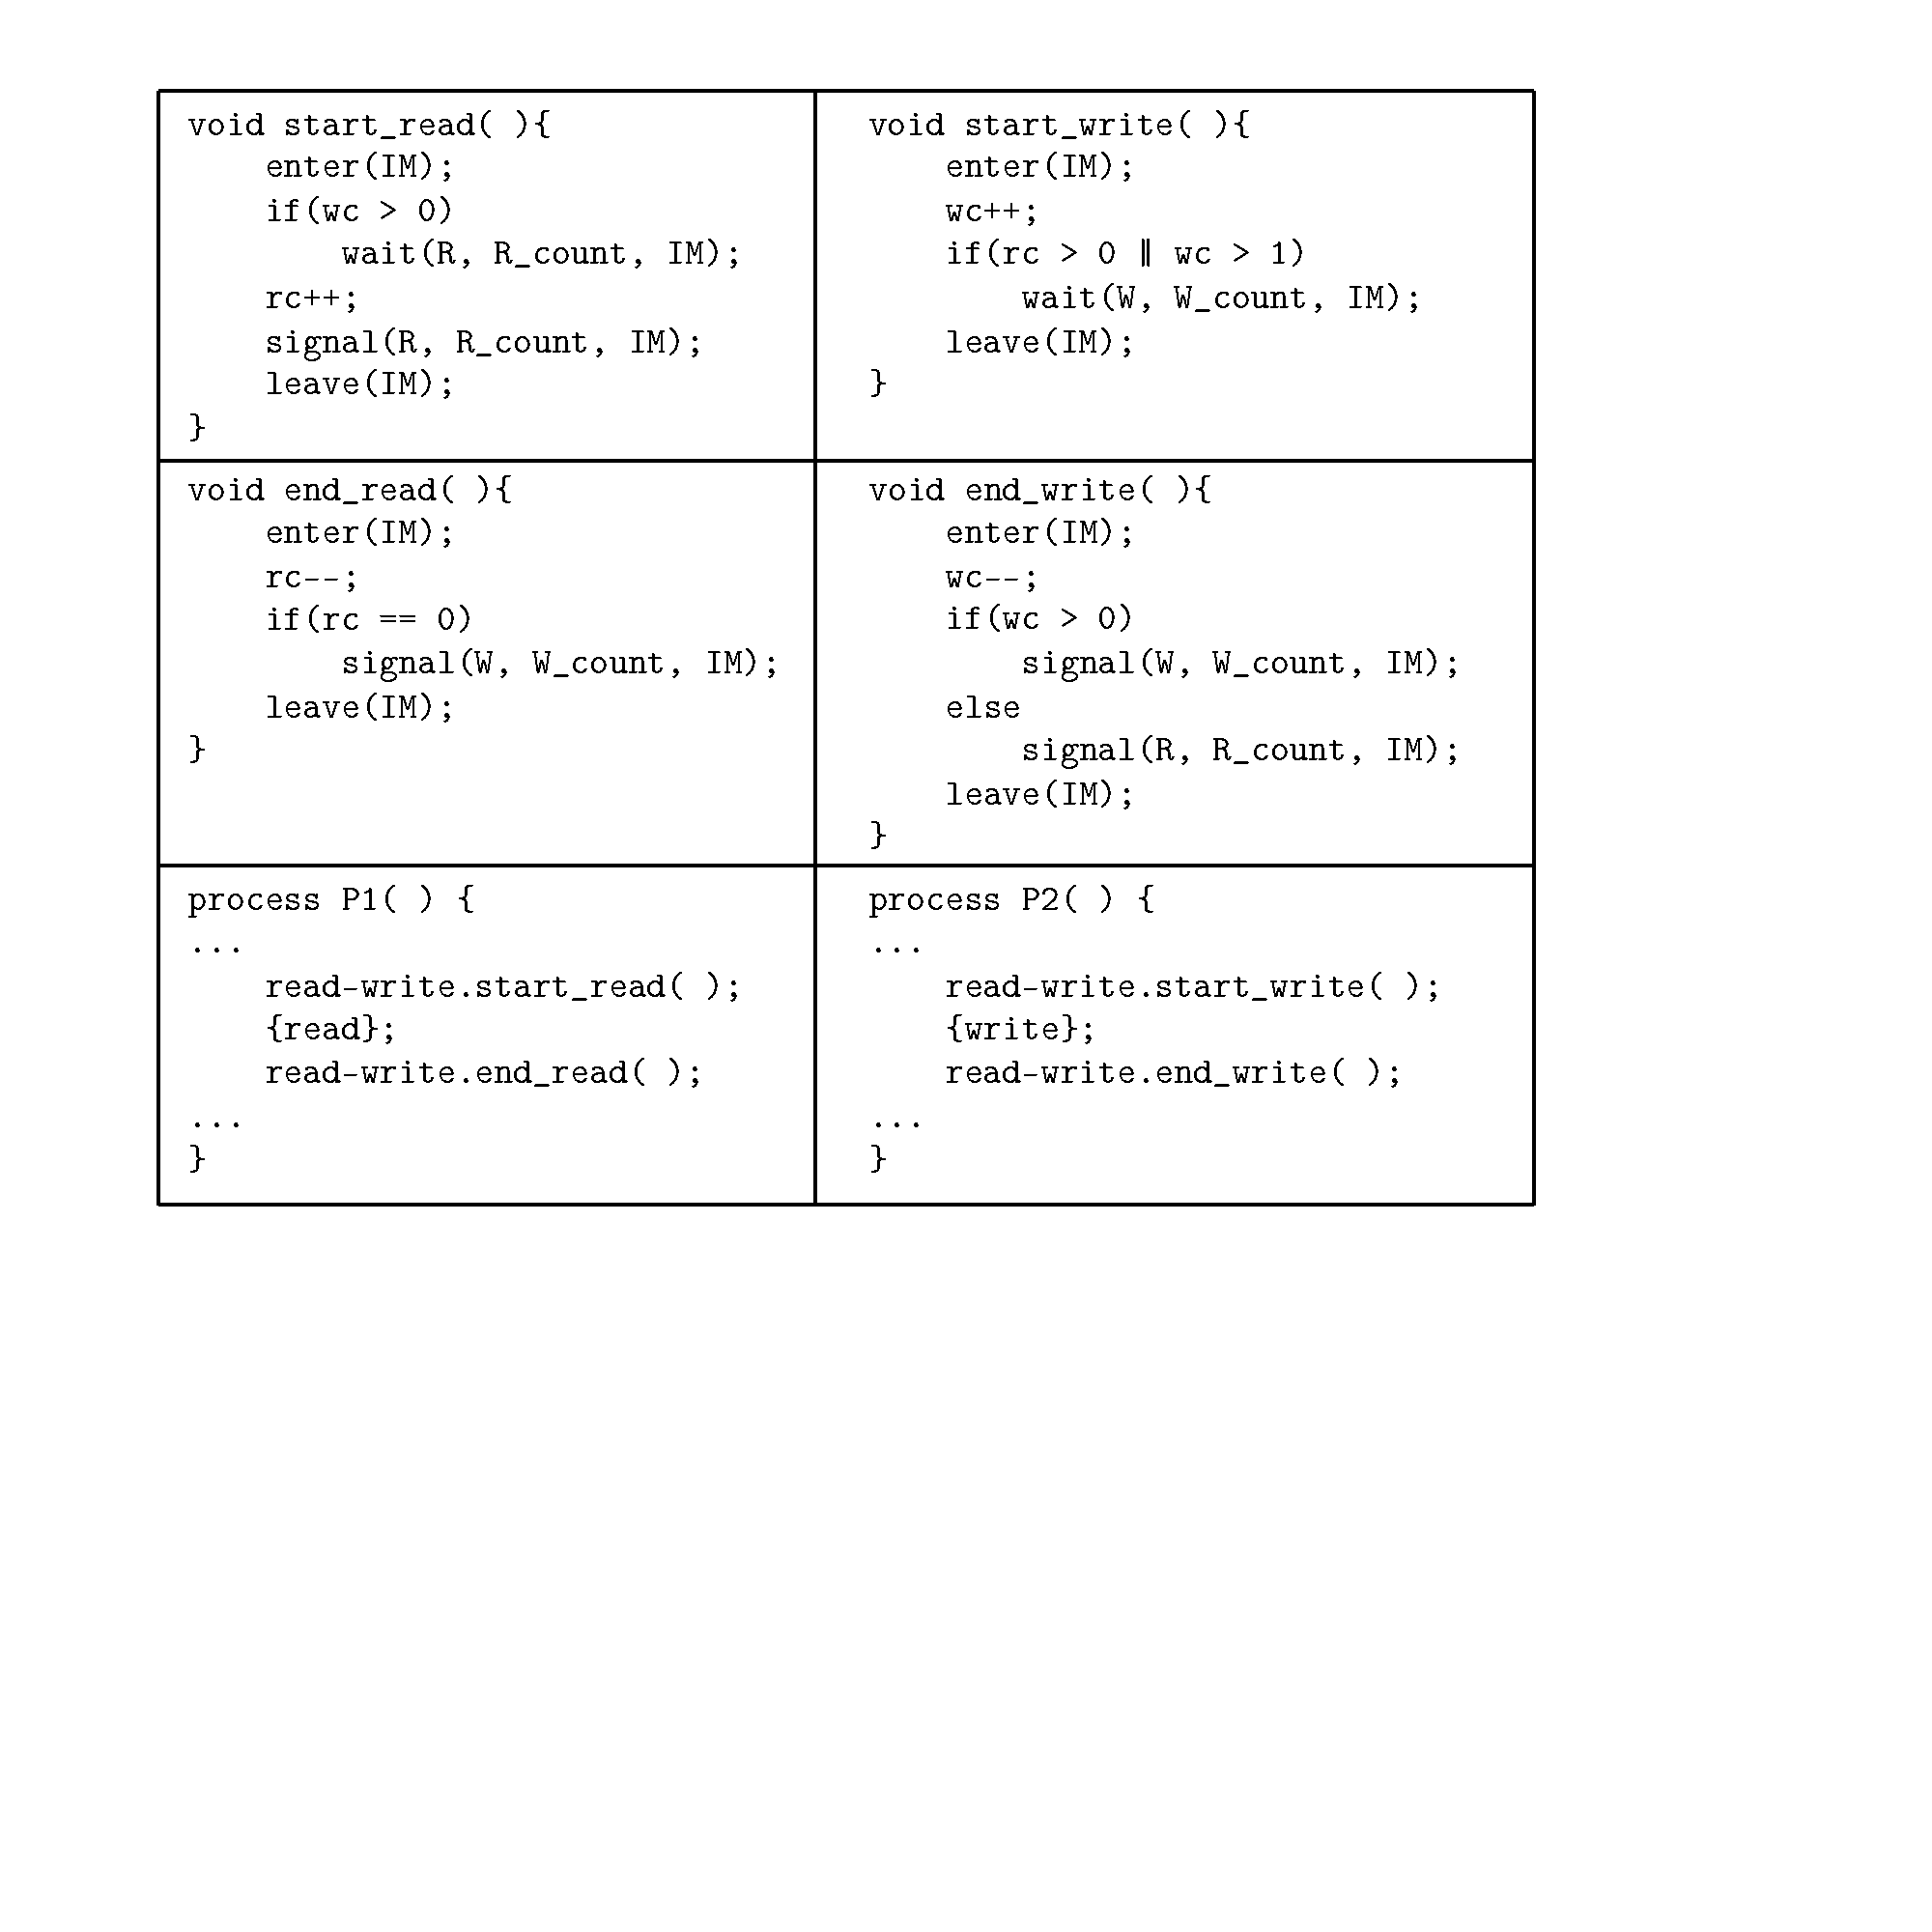
\includegraphics[width=0.75\textwidth]{img/霍尔管程求解读者写者问题.pdf}
	\end{figure}

	\subsubsection{霍尔管程求解哲学家就餐问题}
	\begin{lstlisting}[language=C, keywordstyle=\color{black}]
type dining_philosophers = monitor
	enum {thinking, hungry, eating} state[5];
	semaphore self[5]; int self_count[5];
	InterfaceModule IM;  for (int i=0; i<5; i++){state[i] = thinking; //初始化,i为进程号}
	define pickup, putdown; 
	use enter, leave, wait, signal;
	\end{lstlisting}

	\begin{figure}[H]
		\centering
		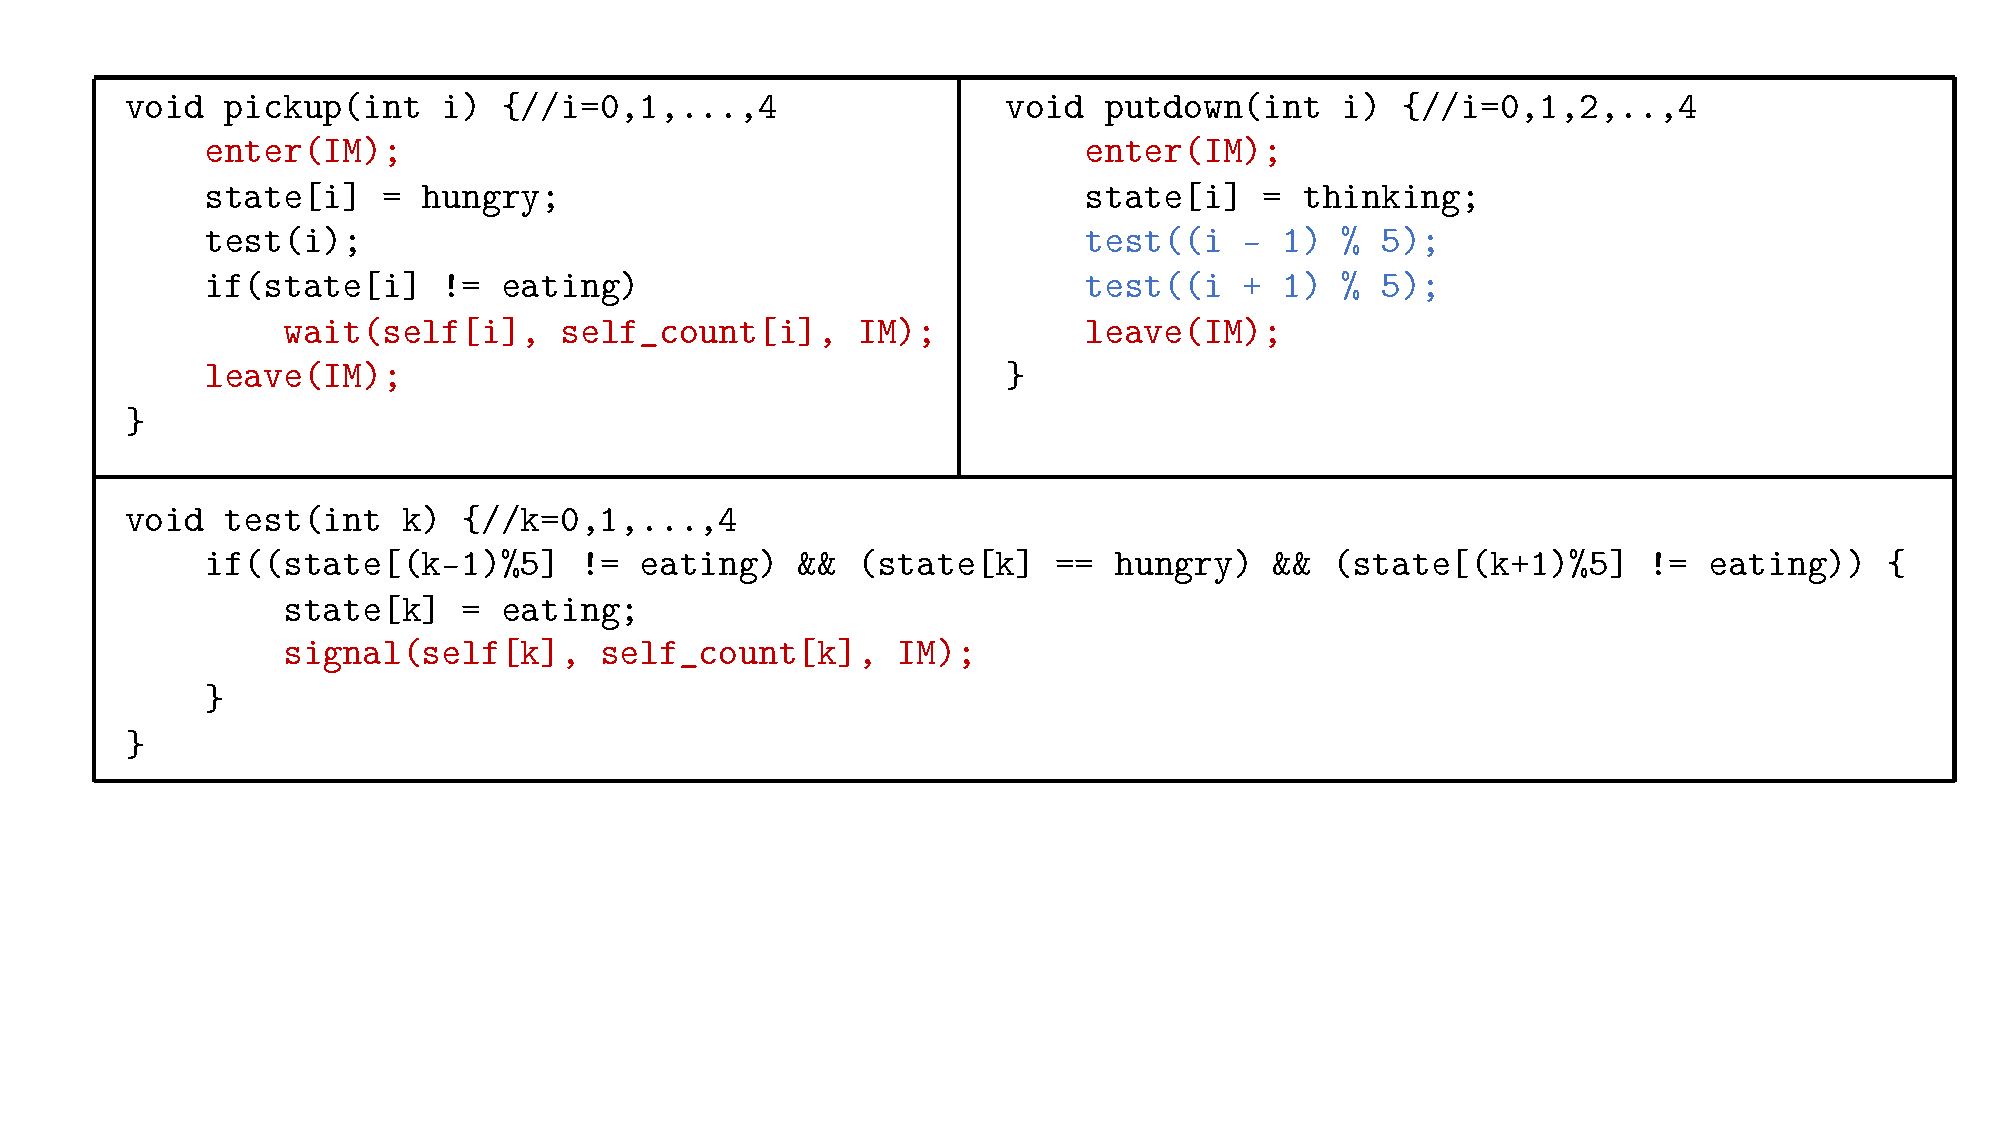
\includegraphics[width=0.98\textwidth]{img/霍尔管程求解哲学家就餐问题.pdf}
	\end{figure}


	\subsubsection{霍尔管程求解生产者消费者问题}
	\begin{lstlisting}[language=C, keywordstyle=\color{black}]
type producer_consumer = monitor
	item B[k]; int in, out; //B[k]表示缓冲单元,in和out是存取指针 
	int count; //缓冲中产品数
	semaphore notfull, notempty; //条件变量
	int notfull_count, notempty_count;
	InterfaceModule IM;
	define append, take;
	use enter, leave, wait, signal;
	\end{lstlisting}

	\begin{figure}[H]
		\centering
		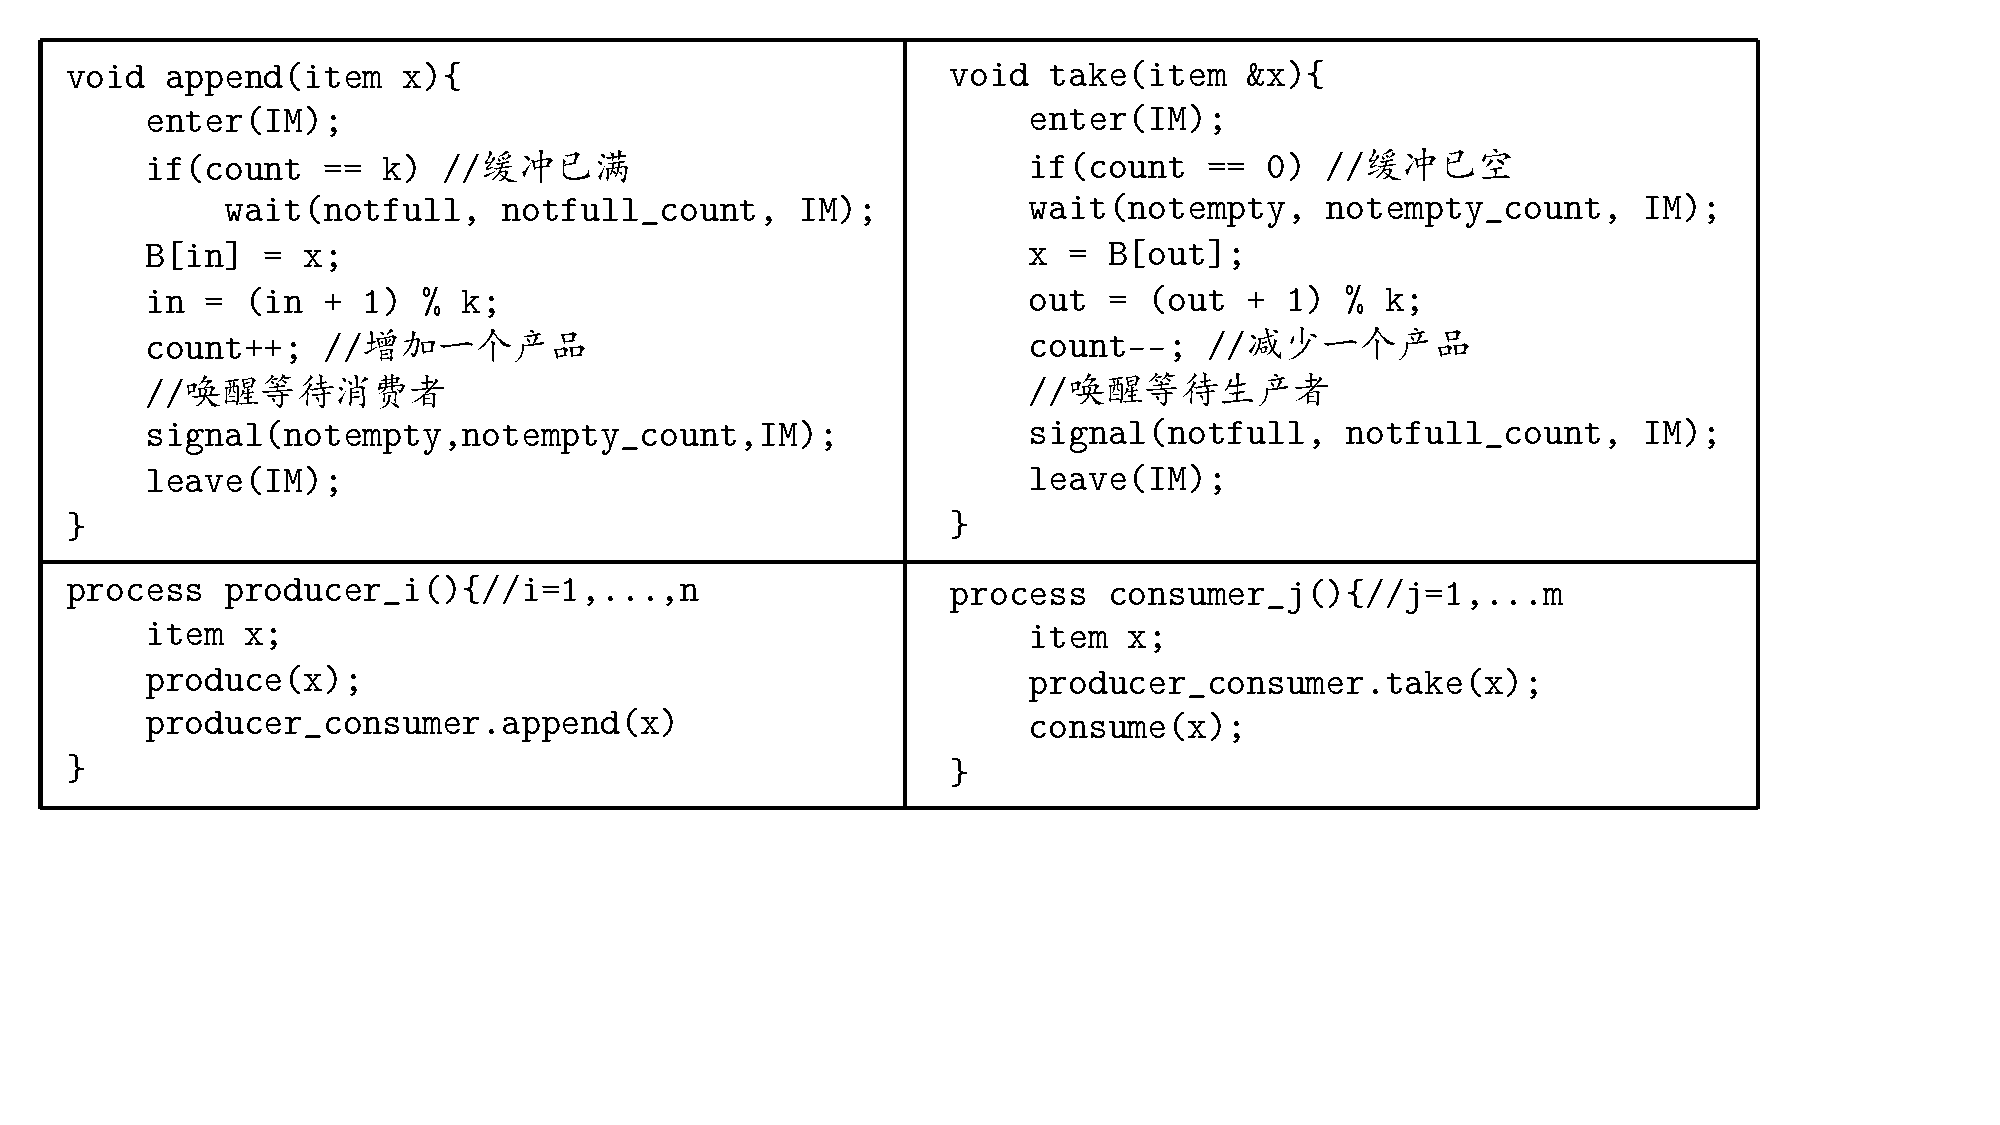
\includegraphics[width=0.98\textwidth]{img/霍尔管程求解生产者消费者问题.pdf}
	\end{figure}


	\subsubsection{霍尔管程求解苹果桔子问题}
	\begin{lstlisting}[language=C, keywordstyle=\color{black}]
type FMSD = monitor
	enum FRUIT {apple, orange} plate; bool full;
	semaphore SP, SS, SD; int SP_count, SS_count, SD_count; full = false
	InterfaceModule IM;
	define put, get;
	use enter, leave, wait, signal;
	\end{lstlisting}

	\begin{figure}[H]
		\centering
		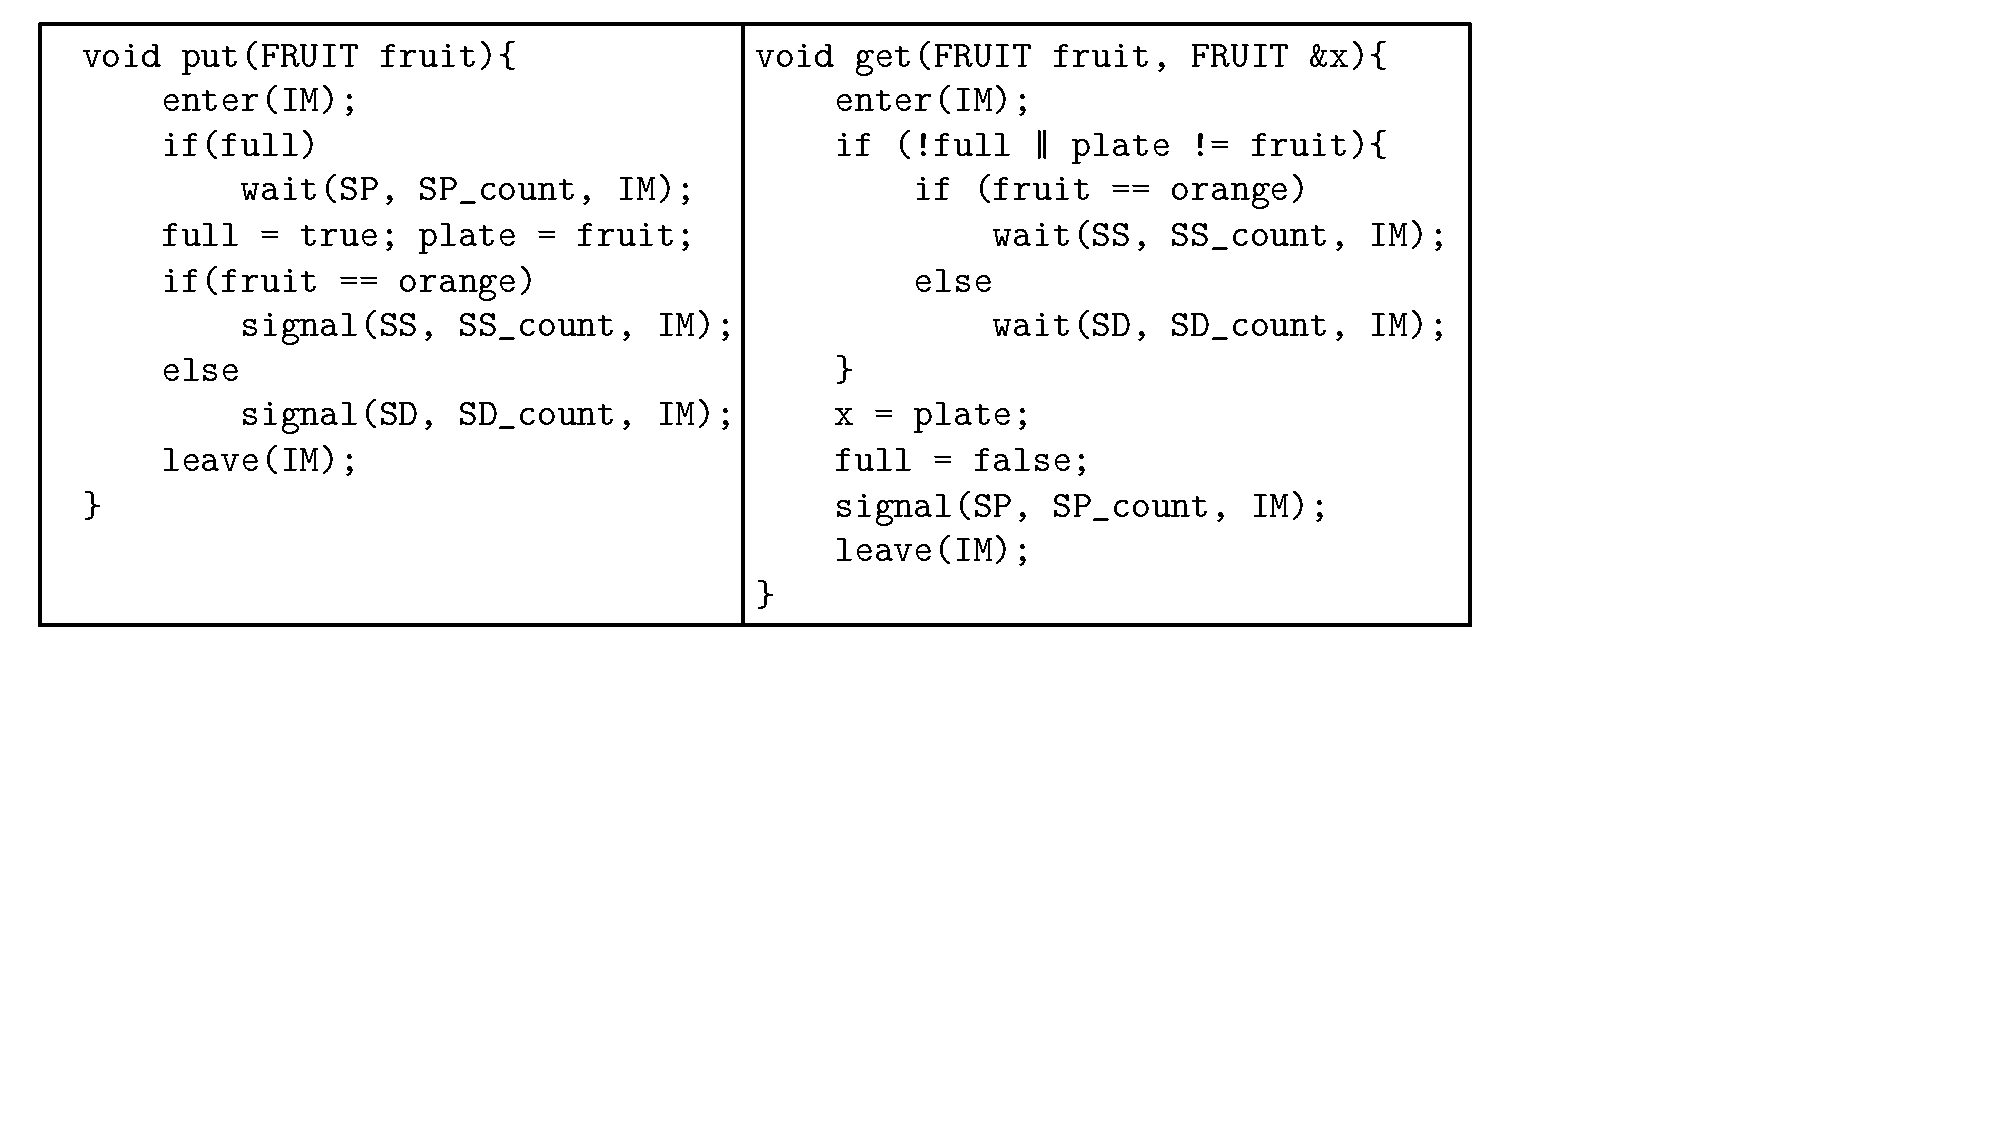
\includegraphics[width=0.98\textwidth]{img/霍尔管程求解苹果桔子问题1.pdf}
	\end{figure}

	\begin{figure}[H]
		\centering
		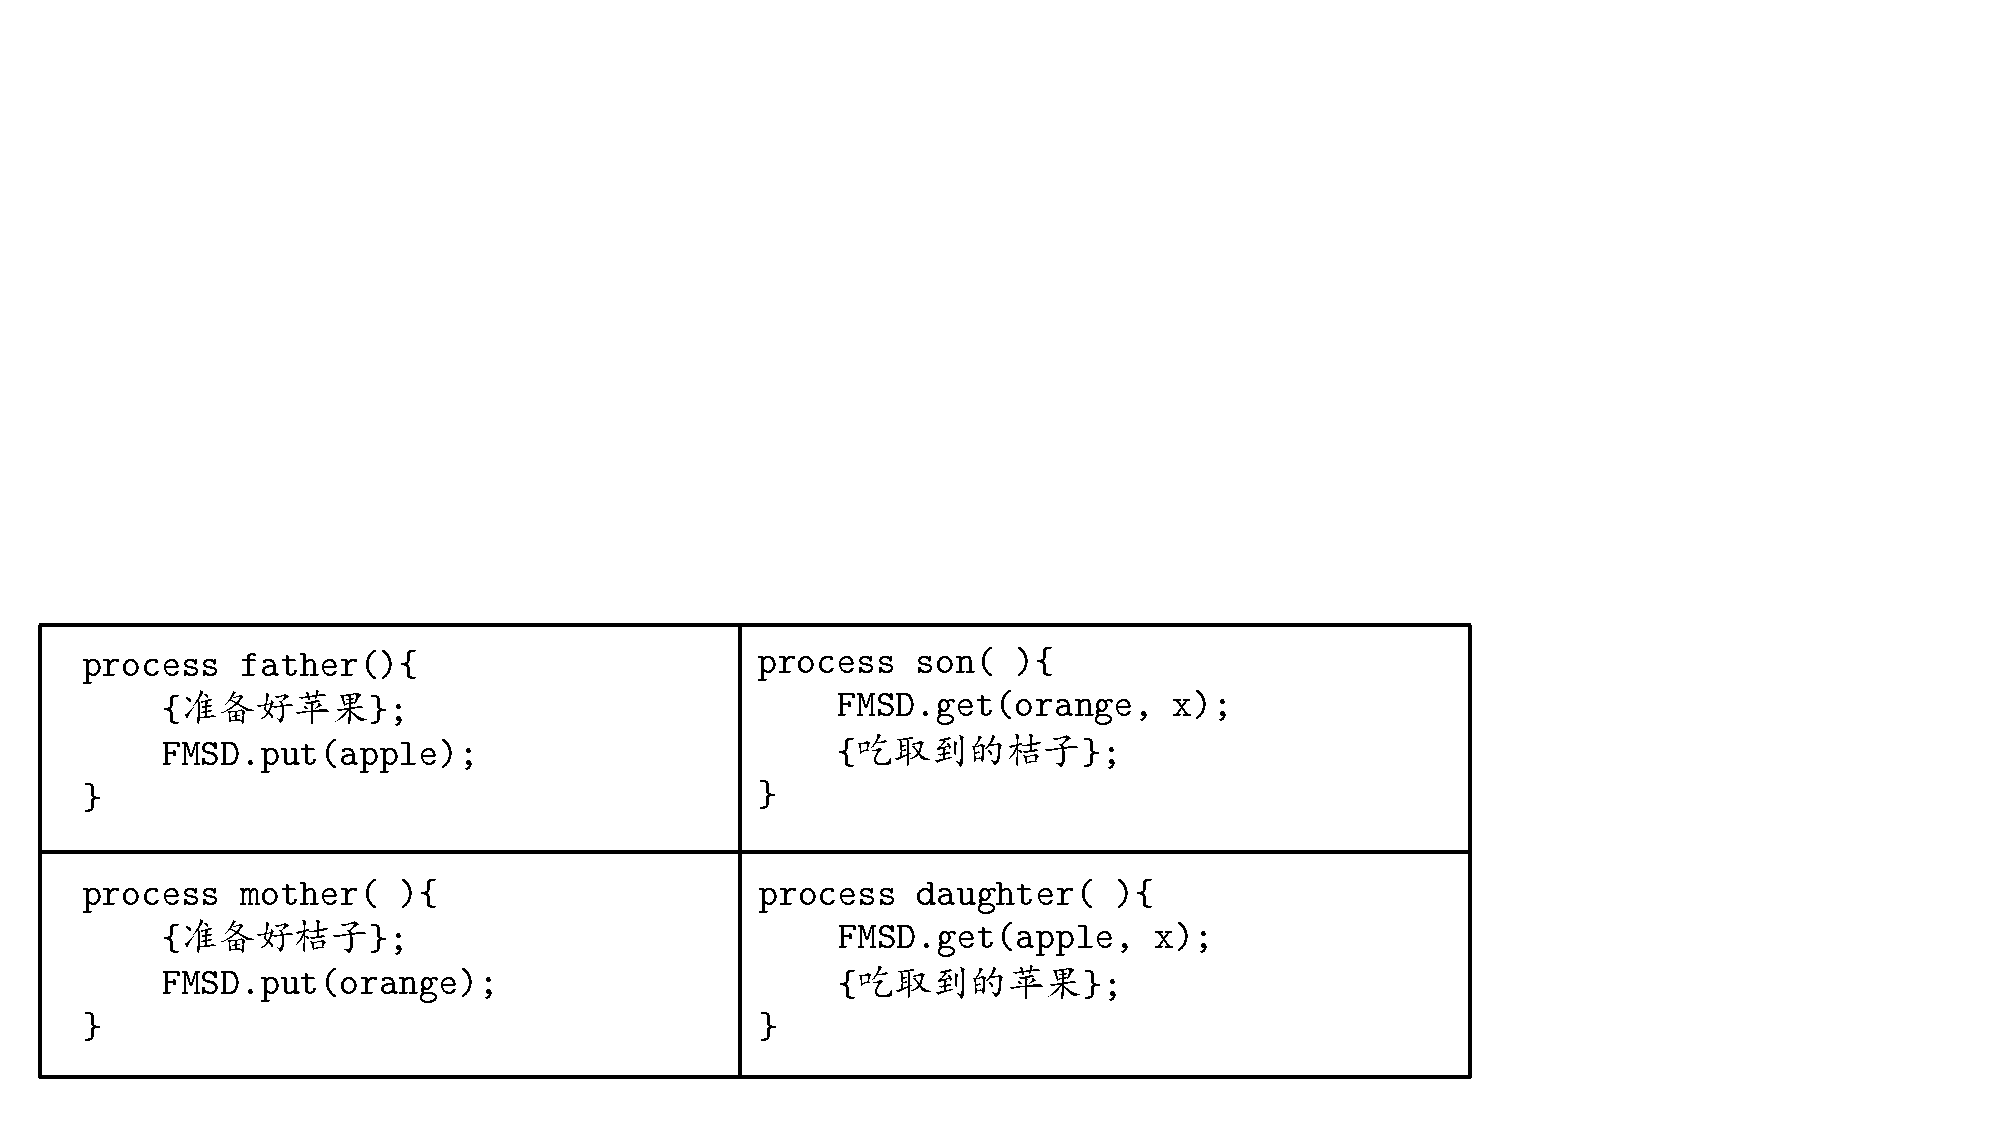
\includegraphics[width=0.98\textwidth]{img/霍尔管程求解苹果桔子问题2.pdf}
	\end{figure}

	\section{进程通信}
	\subsection{进程通信概述}
	交往进程通过信号量操作实现进程互斥和同步,这是一种低级通信方式

	进程有时还需要交换更多的信息(如把数据传送给另一个进程),为此可以引进高级通信方式:进程通信机制,实现进程间用信件来交换信息,进程通信扩充了并发进程的数据共享
	\begin{itemize}
		\item 通过该通信机制,一个正在执行的进程可以在任何时刻向另一个正在执行的进程发送或请求信件
		\item 如果一个进程在某一时刻的执行依赖于另一进程的信件或等待其他进程对发送信件的回答,那么通信机制将与进程阻塞和释放紧密联系
		\item 这样,进程间的通信就进一步扩充了并发进程间对数据的共享
	\end{itemize}


	\subsubsection{进程直接通信}
	在进程直接通信方式下,企图发送或接收消息的每个进程必须指出信件发给谁或从谁那里接收信件,可用下面两条原语来实现进程之间的通信
	\begin{itemize}
		\item \verb|send(P, 信件)|:将信件发送给进程P
		\item \verb|receive(Q, 信件)|:从进程Q接收信件
	\end{itemize}

	\begin{figure}[H]
		\centering
		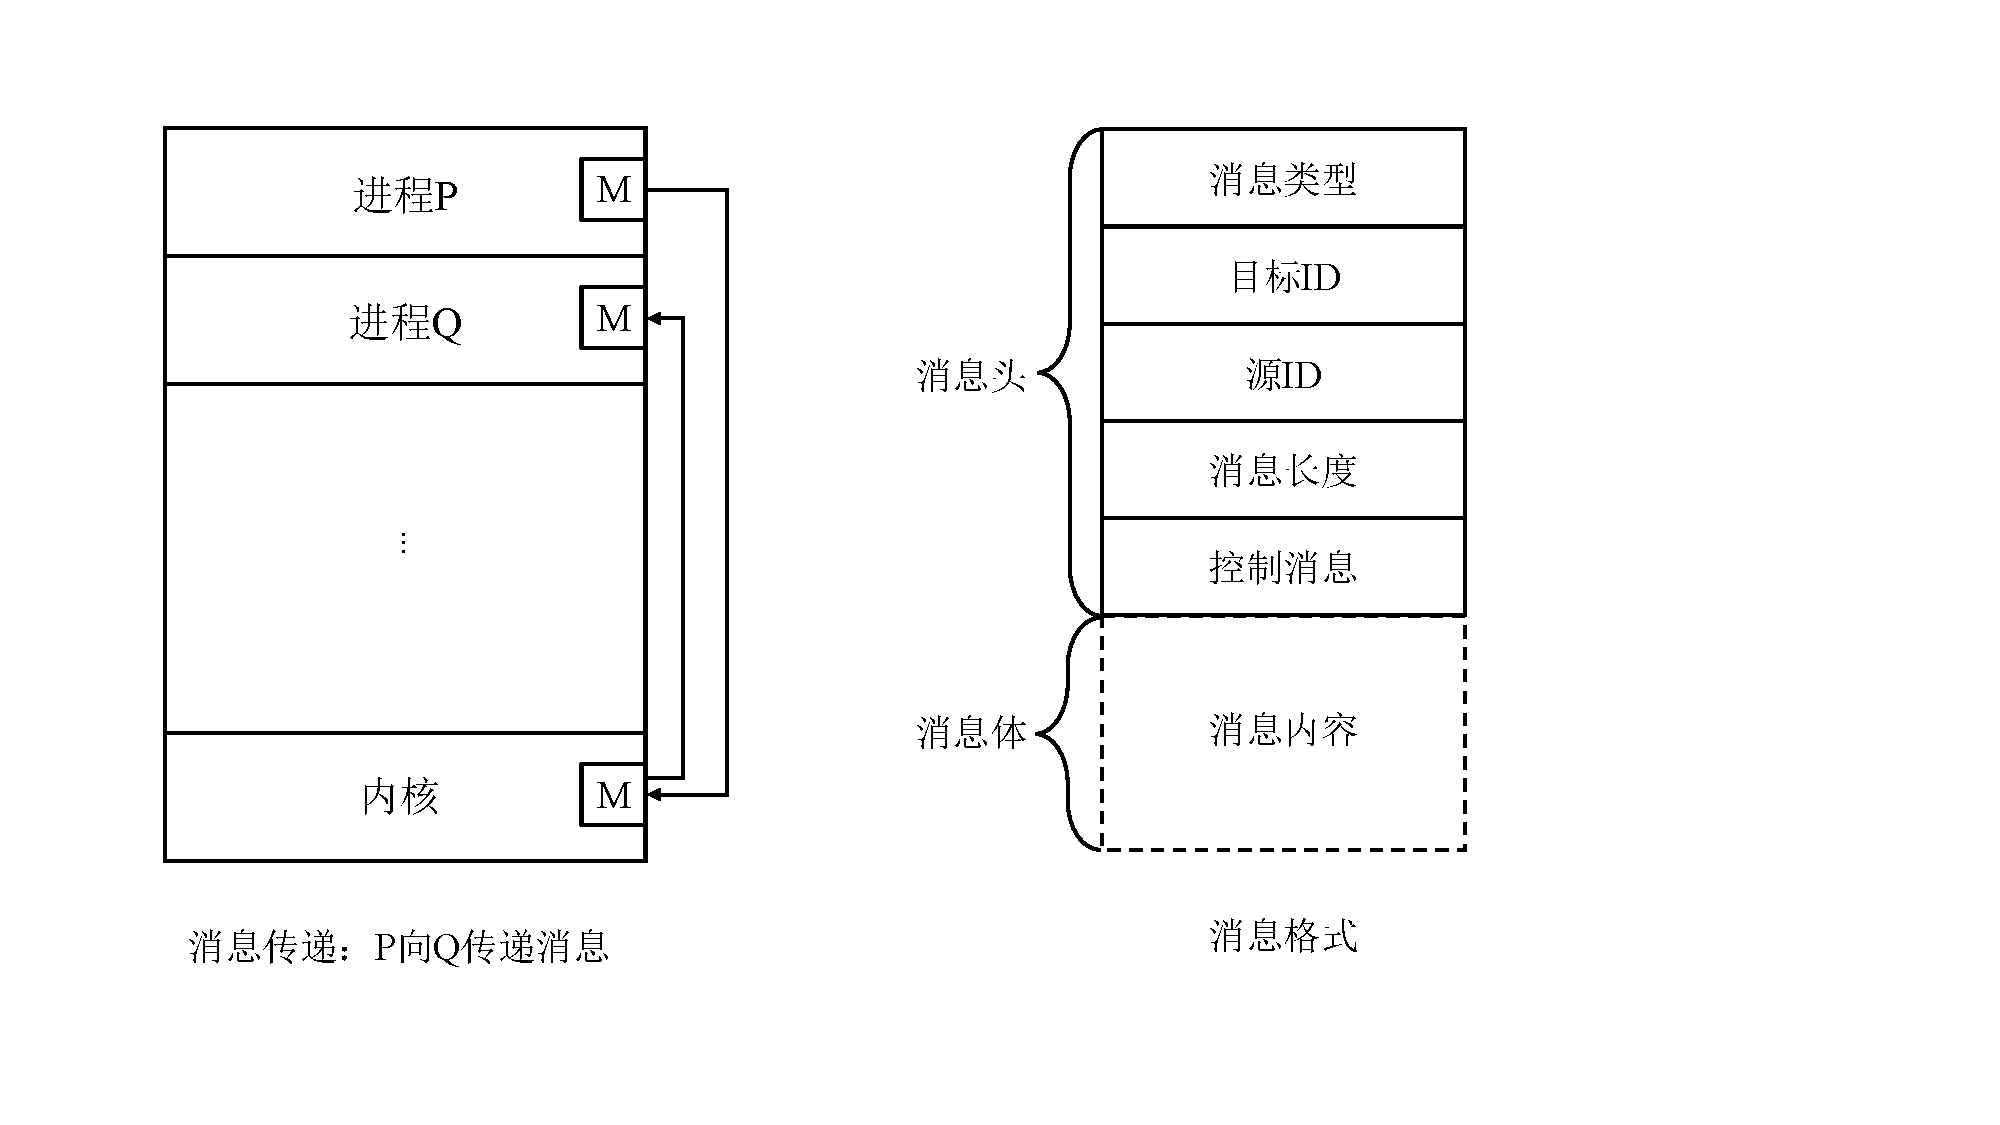
\includegraphics[width=0.5\textwidth]{img/进程直接传递和消息格式.pdf}
	\end{figure}
	
	\subsubsection{进程间接通信}
	对于间接通信方式,进程间发送或接收信件通过一个共享的数据结构——信箱来进行,每个信箱有一个唯一的标识符
	\begin{itemize}
		\item 信箱是存放信件的存储区域,可以分成信箱头和信箱体两部分
		\begin{itemize}
			\item 信箱头指出信箱容量、信件格式、存放信件位置的指针等
			\item 信箱体用来存放信件,信箱体分成若干个区,每个区可容纳一封信
		\end{itemize}
		\item 当两个以上的进程共享一个信箱时,它们之间通过共享的信箱进行通信
	\end{itemize}

	间接通信方式中的发送和接收原语形式如下:
	\begin{itemize}
		\item \verb|send(A,信件)|:将信件发送到信箱A
		\item \verb|receive(A,信件)|:从信箱A接收信件
	\end{itemize}

	发送和接收两条原语的功能如下:
	\begin{itemize}
		\item 发送信件:如果指定的信箱末满,则将信件送入信箱中由指针所指示的位置,并释放等待该信箱中信件的等待者;否则,发送信件者被置成等待信箱状态
		\item 接收信件:如果指定信箱中有信,则取出一封信件,并释放等待信箱的等待者;否则,接收信件者被置成等待信箱中信件的状态
	\end{itemize}

	\verb|send/receive|原语的算法描述:
	\begin{figure}[H]
		\centering
		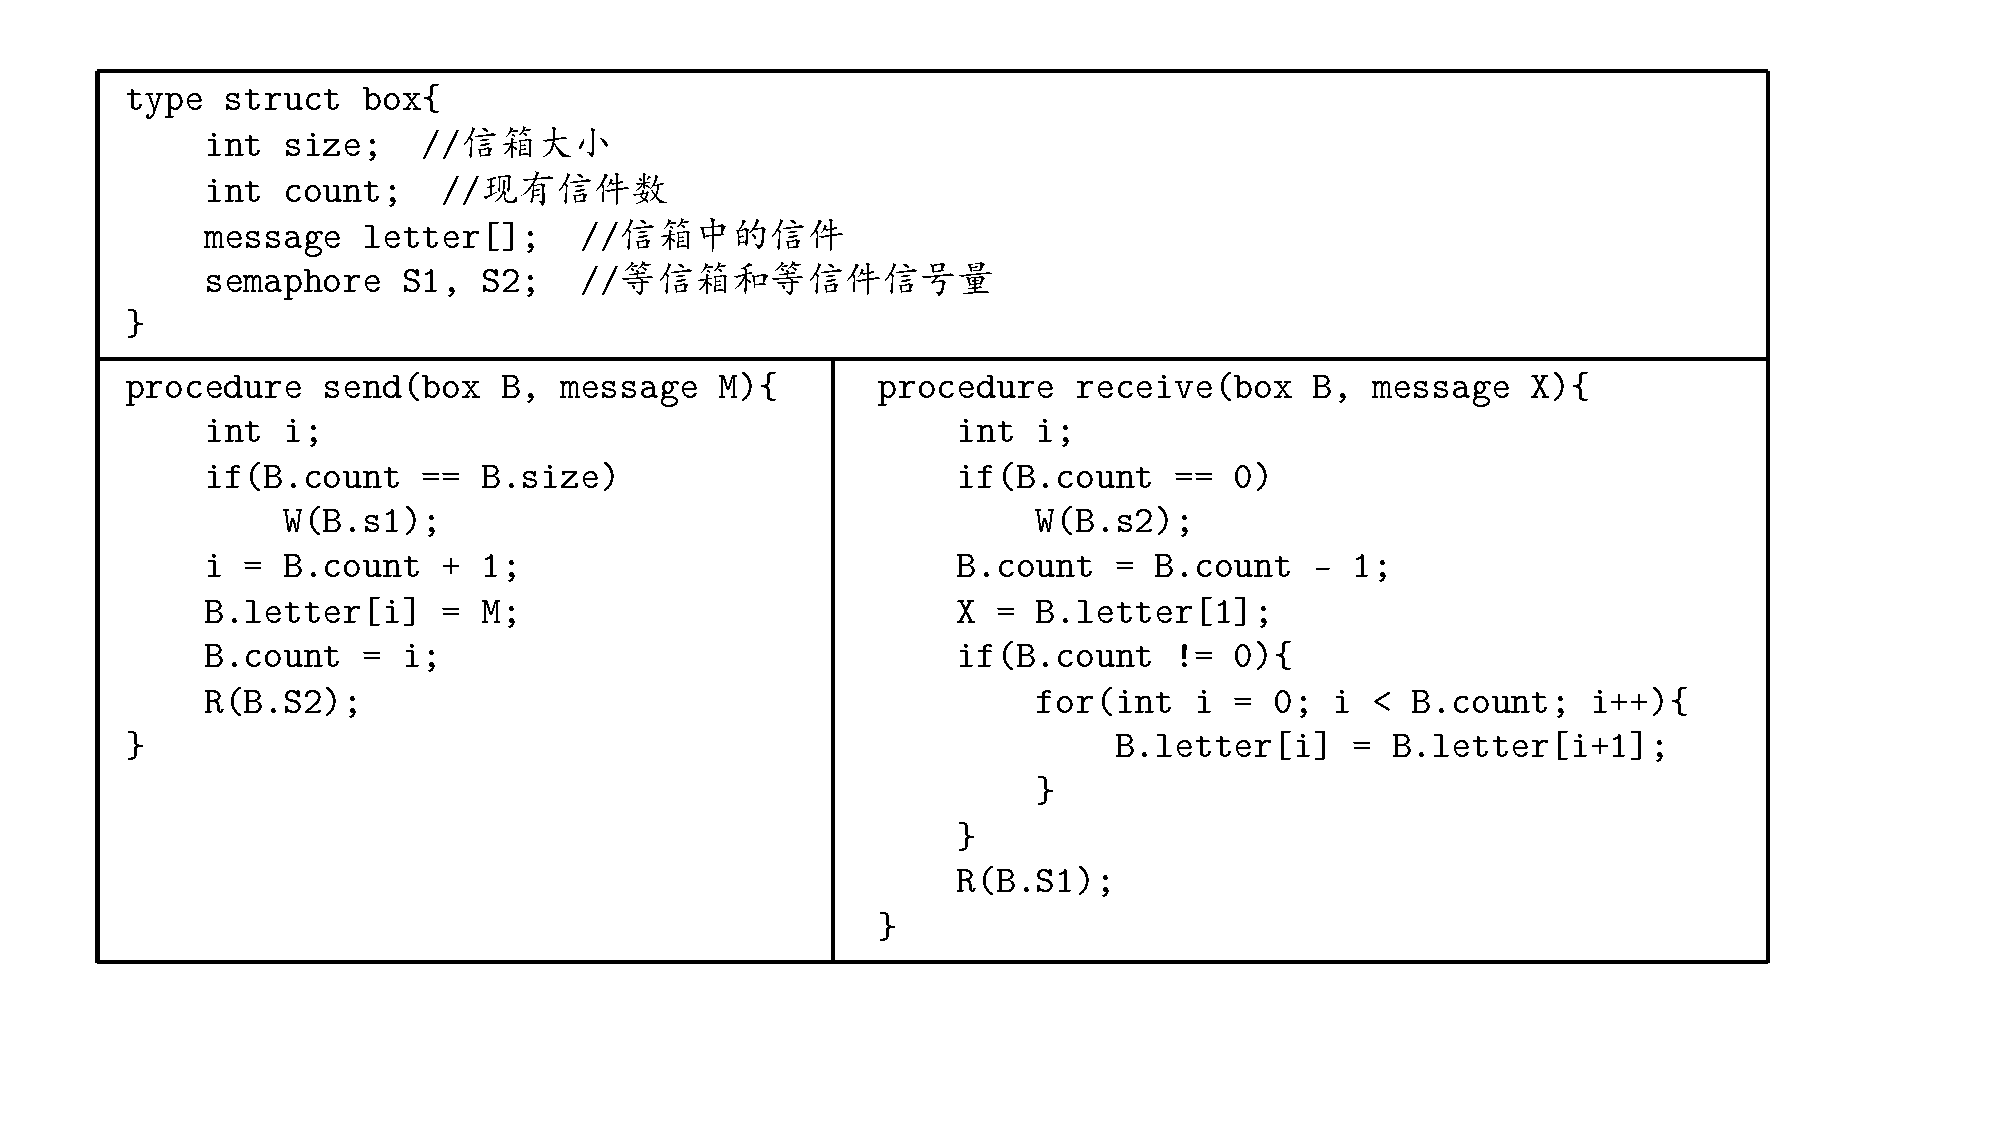
\includegraphics[width=0.95\textwidth]{img/send receive原语的算法描述.pdf}
	\end{figure}

	利用消息传递求解生产者消费者问题
	\begin{lstlisting}[language=C, keywordstyle=\color{black}]
creat_mailbox(producer); //创建信箱
creat_mailbox(consumer);

void producer_i(){ //i=1,...,n
	message pmsg;
	while(true){
		pmsg = produce(); 
		send(consumer, pmsg);
	} 
}

void consumer_j(){ //j=1,...,m
	message cmsg;
	while(true){
	receive (consumer, cmsg);
	consume(csmg); 
	}
}

cobegin
	producer_i();
	consumer_j();
coend
	\end{lstlisting}

	\subsubsection{消息缓冲通信}
	消息缓冲是在1973年由P.B.Hansan提出的一种进程间高级通信设施,并在RC4000系统中实现

	消息缓冲通信的基本思想:
	\begin{itemize}
		\item 由操作系统统一管理一组用于通信的消息缓冲存储区,每一个消息缓冲存储区可存放一个消息(信件)
		\item 当一个进程要发送消息时,先在自己的消息发送区里生成待发送的消息,包括:接收进程名、消息长度、消息正文等
		\item 然后,向系统申请一个消息缓冲区,把消息从发送区复制到消息缓冲区中,注意在复制过程中系统会将接收进程名换成发送进程名,以便接收者识别
		\item 随后该消息缓冲区被挂到接收消息的进程的消息队列上,供接收者在需要时从消息队列中摘下并复制到消息接收区去使用,同时释放消息缓冲区
	\end{itemize}

	消息缓冲通信涉及的数据结构:
	\begin{itemize}
		\item \verb|sender|:发送消息的进程名或标识符
		\item \verb|size|:发送的消息长度
		\item \verb|text|:发送的消息正文
		\item \verb|next-ptr|:指向下一个消息缓冲区的指针
	\end{itemize}

	在进程的PCB中涉及通信的数据结构:
	\begin{itemize}
		\item \verb|mptr|:消息队列队首指针
		\item \verb|mutex|:消息队列互斥信号量,初值为1
		\item \verb|sm|:表示接收进程消息队列上消息的个数,初值为0,是控制收发进程同步的信号量
	\end{itemize}

	发送原语和接收原语的实现如下:
	\begin{itemize}
		\item 发送原语\verb|Send|:申请一个消息缓冲区,把发送区内容复制到这个缓冲区中;找到接收进程的PCB,执行互斥操作\verb|P(mutex)|;把缓冲区挂到接收进程消息队列的尾部,执行\verb|V(sm)|,即消息数加1;执行\verb|V(mutex)|
		\item 接收原语\verb|Receive|:执行\verb|P(sm)|查看是否有信件;执行互斥操作\verb|P(mutex)|,从消息队列中摘下第一个消息,执行\verb|V(mutex)|;把消息缓冲区内容复制到接收区,释放消息缓冲区
	\end{itemize}

	\begin{figure}[H]
		\centering
		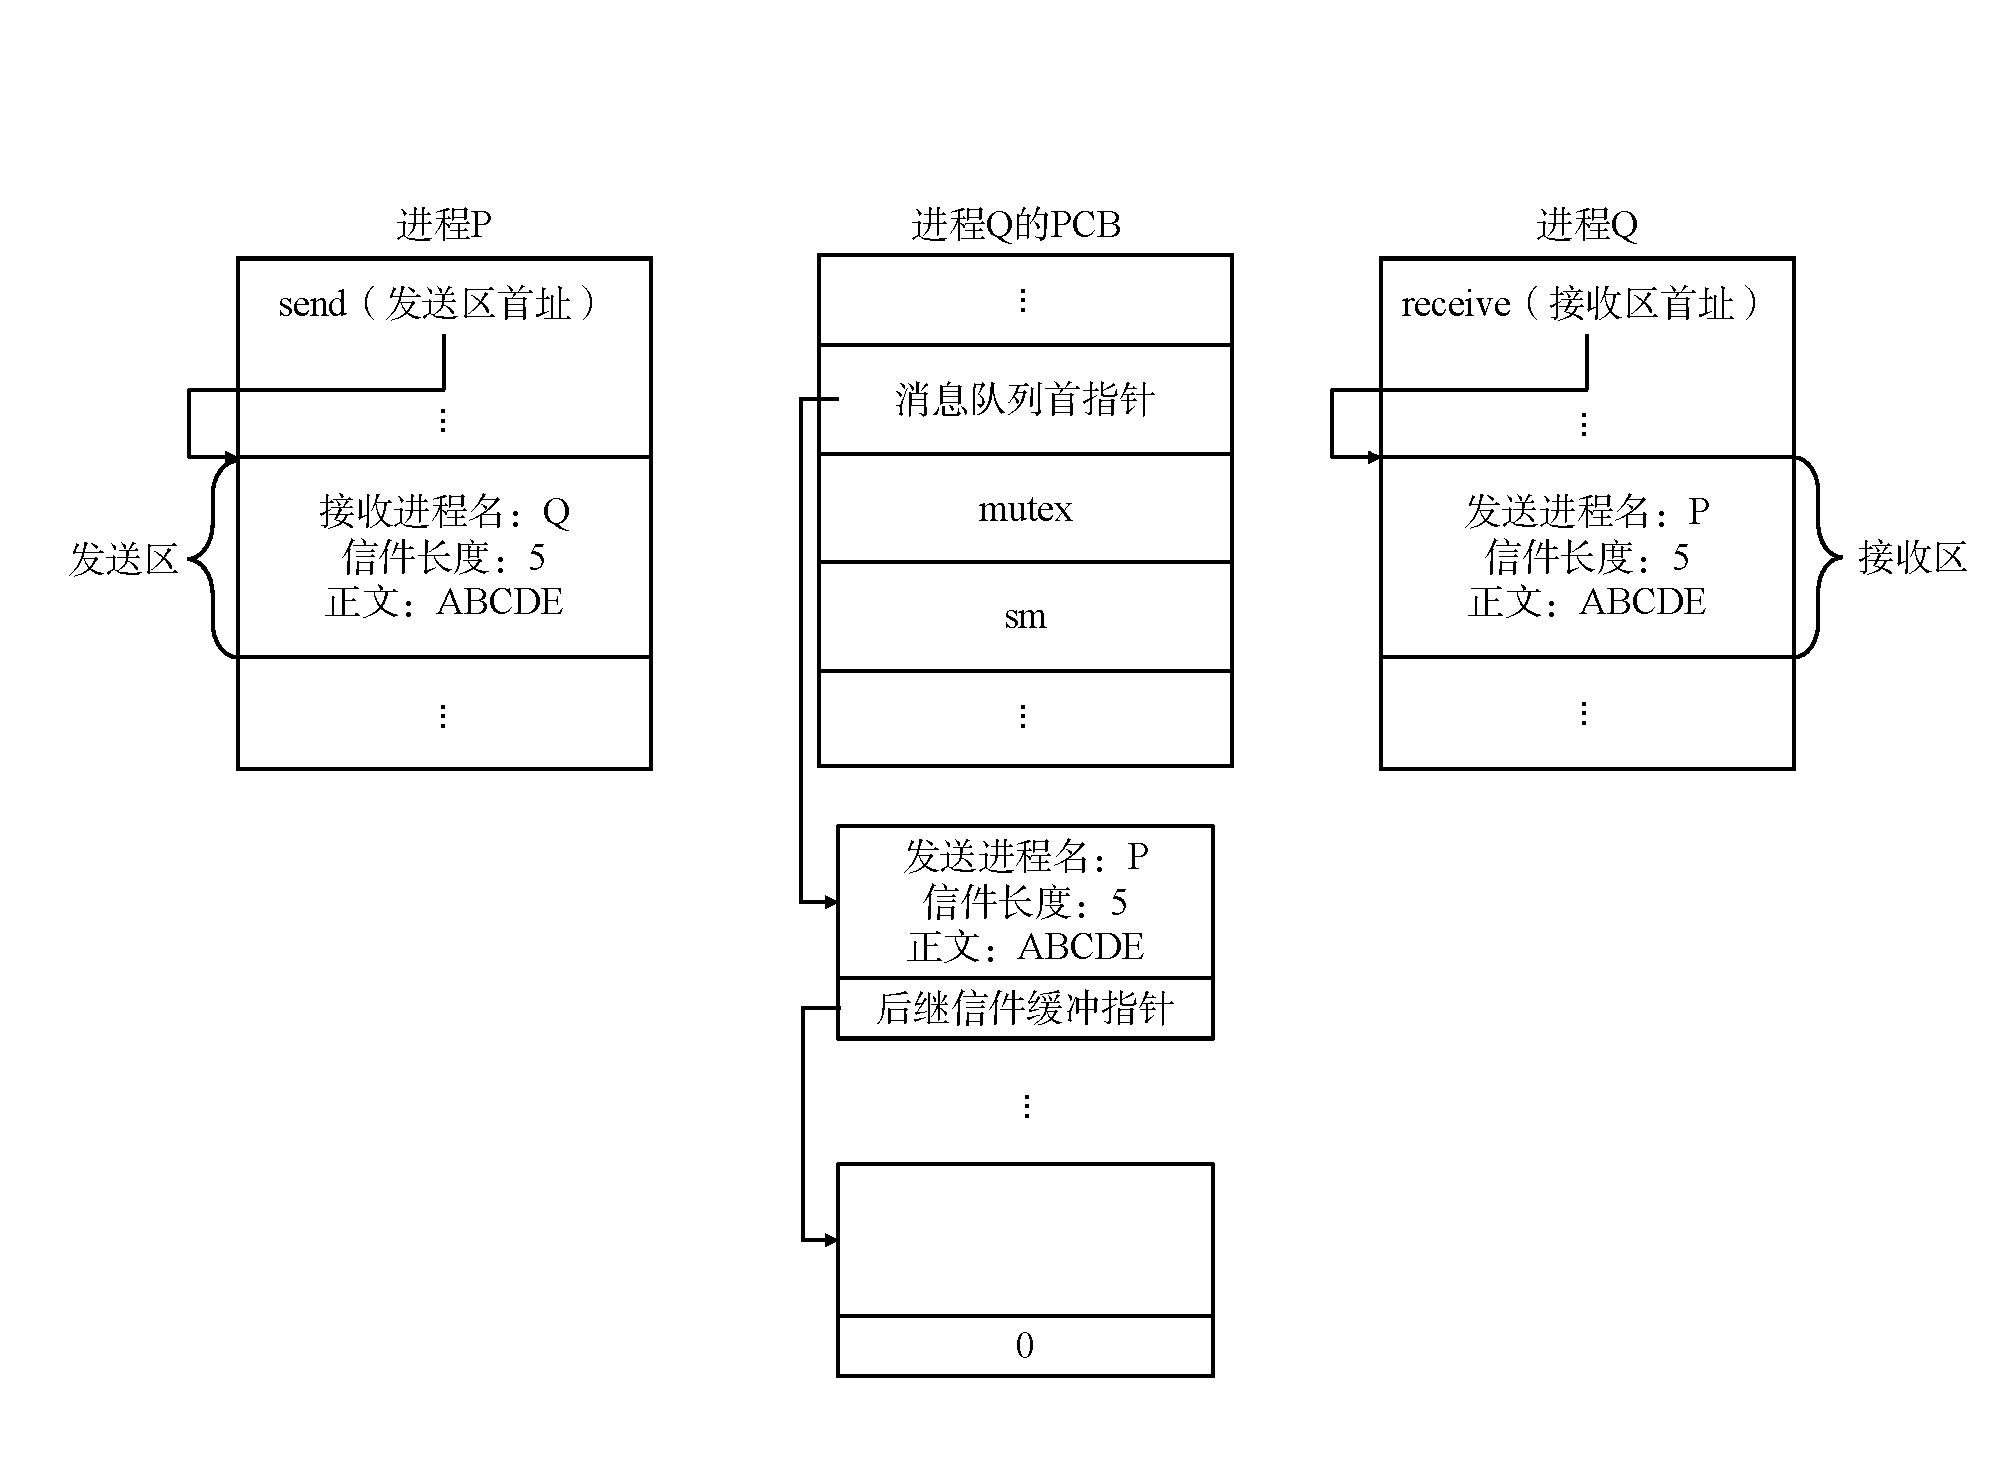
\includegraphics[width=0.85\textwidth]{img/消息缓冲通信.pdf}
	\end{figure}

	\subsubsection{管道和套接字}
	\begin{itemize}
		\item 管道是Unix和C的传统通信方式
		\item 套接字起源于Unix BSD版本,目前已经被Unix和Windows操作系统广泛采用,并支持TCP/IP 协议,即支持本机的进程间通信,也支持网络级的进程间通信
		\item 管道和套接字都是基于信箱的消息传递方式的一种变体,它们与传统的信箱方式等价,区别在于没有预先设定消息的边界。换言之,如果一个进程发送10条100字节的消息,而另一个进程接收1000个字节,那么接收者将一次获得10条消息
	\end{itemize}


	\subsection{高级进程通信机制}

	\subsubsection{基于流的进程通信}
	\begin{itemize}
		\item 多个进程可以使用一个共享的消息缓冲区,这个缓冲区将被组织成一个字节流,而非一个信件流
		\begin{itemize}
			\item 已有很多操作系统实现了类似的机制,有的称之为管道,有的称之为多路转接器,有的称之为套接字等
		\end{itemize}
		\begin{figure}[H]
			\centering
			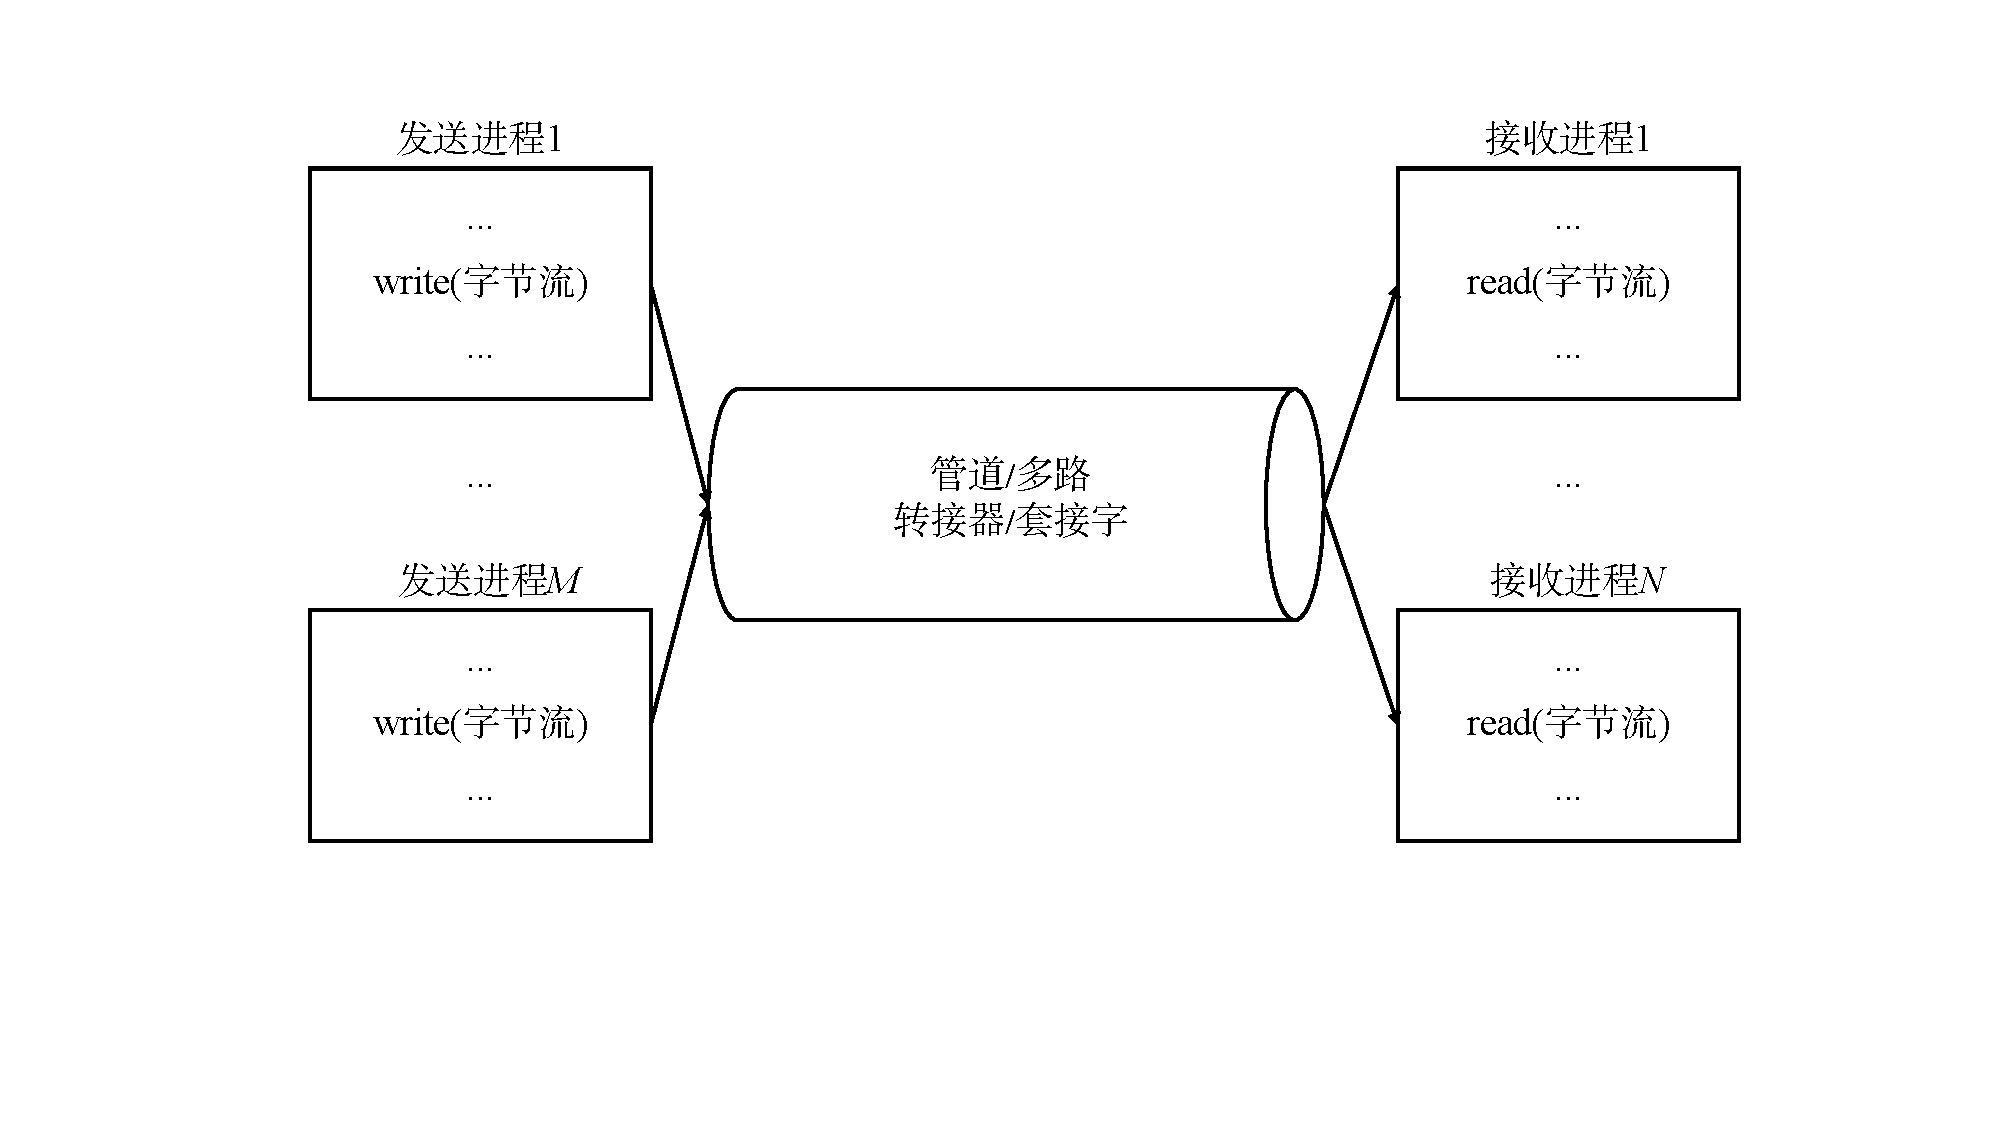
\includegraphics[width=0.6\textwidth]{img/基于流的进程通信.pdf}
		\end{figure}
		\item 发送者或称为发送消息的进程向消息缓冲区中写入字节流,接收消息的进程则从消息缓沖区中读取字节流
		\item 可以根据需求任意地读出一个字节流,只要消息缓沖区中有足够的字节数,就可以读出来,如果没有足够的字节数,就去等待消息
		\item 发送进程在写入字节流时如果消息缓冲区已满,就需要等待该消息缓冲区
	\end{itemize}
	

	\subsubsection{基于RPC的高级通信规约}
	远程过程调用(RPC)是目前在分布式系统中广泛采用的进程通信方法,它将单机环境下的过程调用拓展到分布式环境中,允许不同计算机上的进程使用简单的过程调用和返回结果的方式进行交互
	\begin{itemize}
		\item 采用客户/服务器计算模式
		\item 服务器进程提供一系列过程/服务,供客户进程调用
		\item 客户进程通过调用服务器进程提供的过程/服务获得服务
		\item 考虑到客户计算机和服务器计算机的硬件异构型,外部数据表示XDR被引入来转换每台计算机的特殊数据格式为标准数据格式
	\end{itemize}

	基于RPC/XDR的高级通信规约
	\begin{figure}[H]
		\centering
		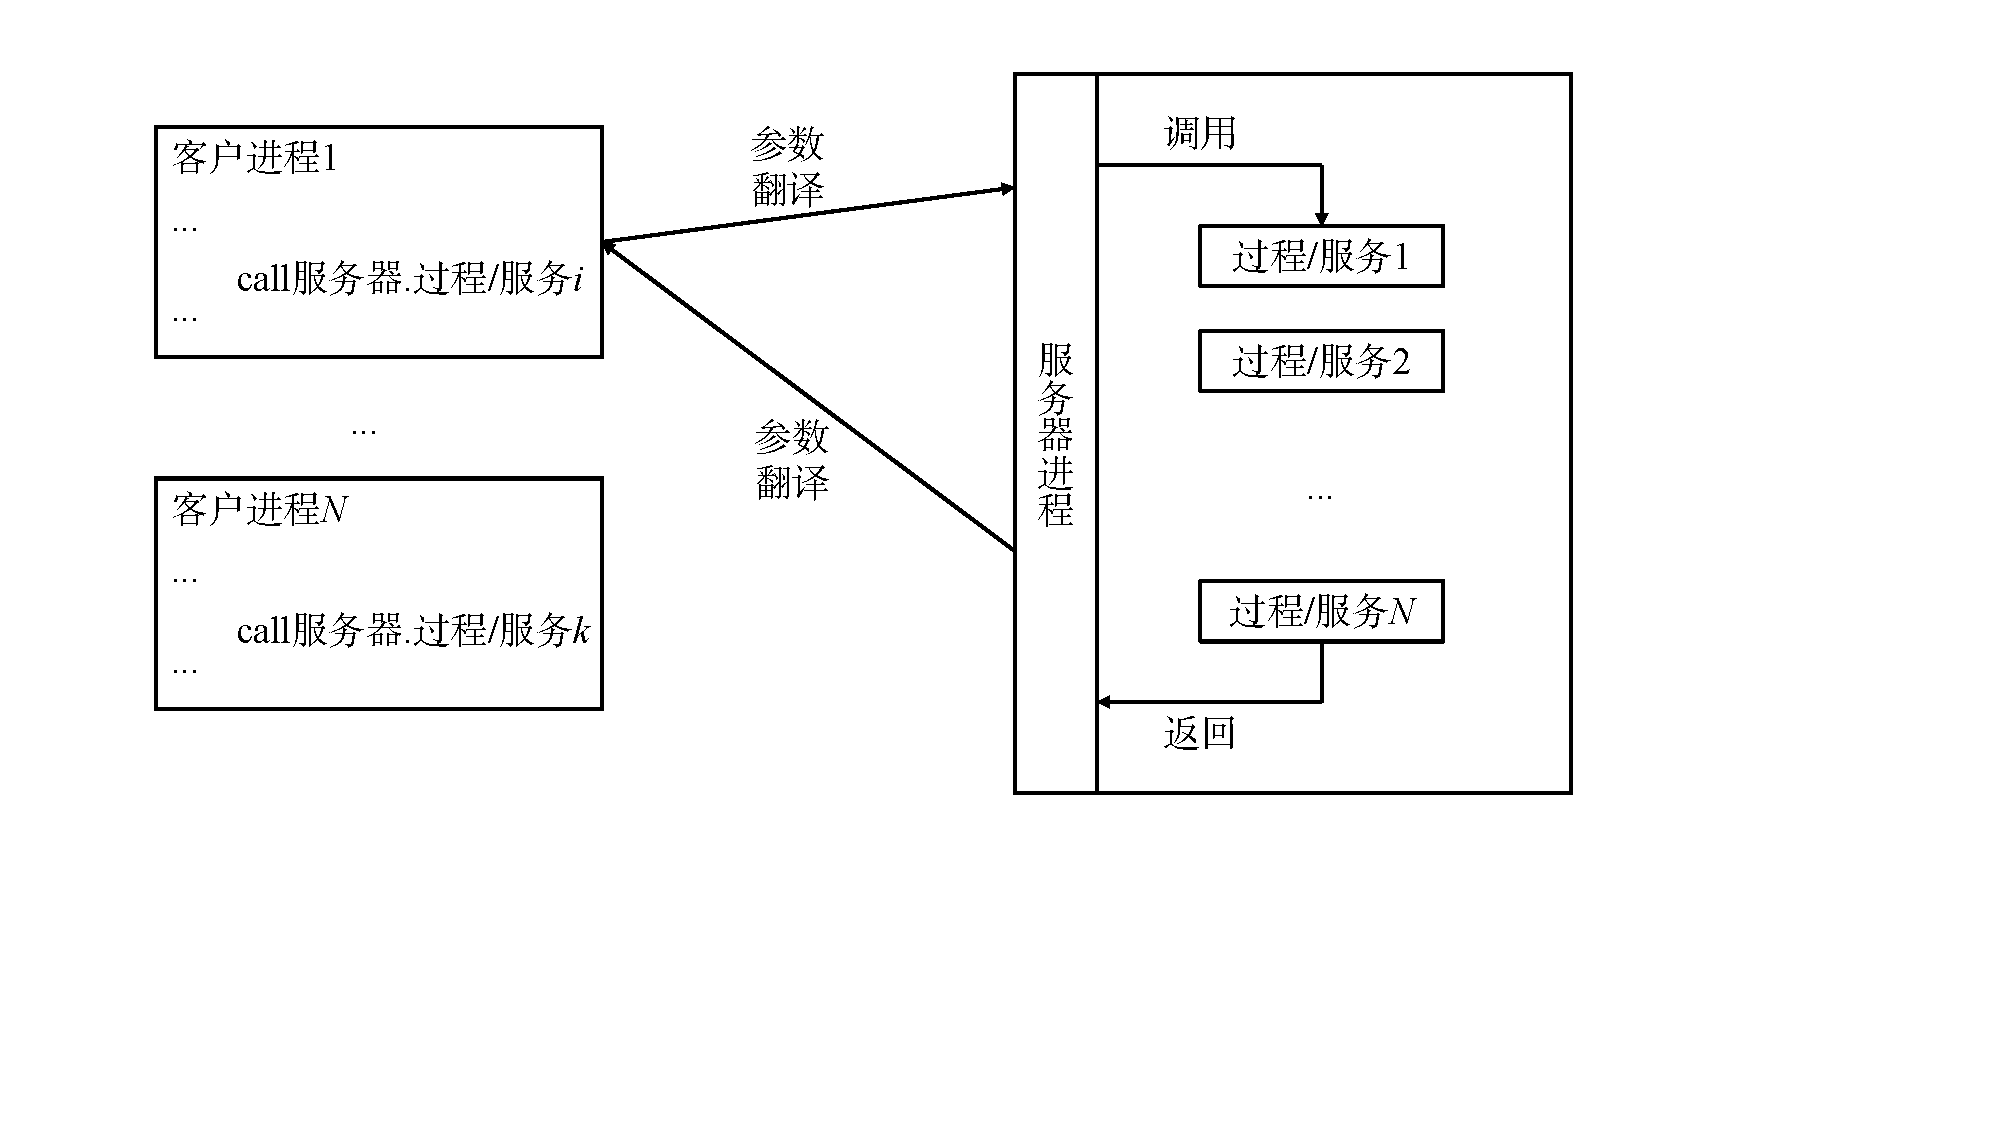
\includegraphics[width=0.75\textwidth]{img/基于RPC XDR的高级通信规约.pdf}
	\end{figure}

	RPC的执行步骤:
	\begin{enumerate}[label=\arabic*.]
		\item 客户进程以普通方式调用客户存根
		\item 客户存根组织RPC消息并执行Send,激活内核程序
		\item 内核把消息通过网络发送到远地内核
		\item 远地内核把消息送到服务器存根
		\item 服务器存根取出消息中参数后调用服务器过程
		\item 服务器过程执行完后把结果返回至服务器存根
		\item 服务器存根进程将它打包并激活内核程序
		\item 服务器内核把消息通过网络发送至客户机内核
		\item 客户内核把消息交给客户存根
		\item 客户存根从消息中取出结果返回给客户进程
		\item 客户进程获得控制权并得到了过程调用的结果
	\end{enumerate}
	\begin{figure}[H]
		\centering
		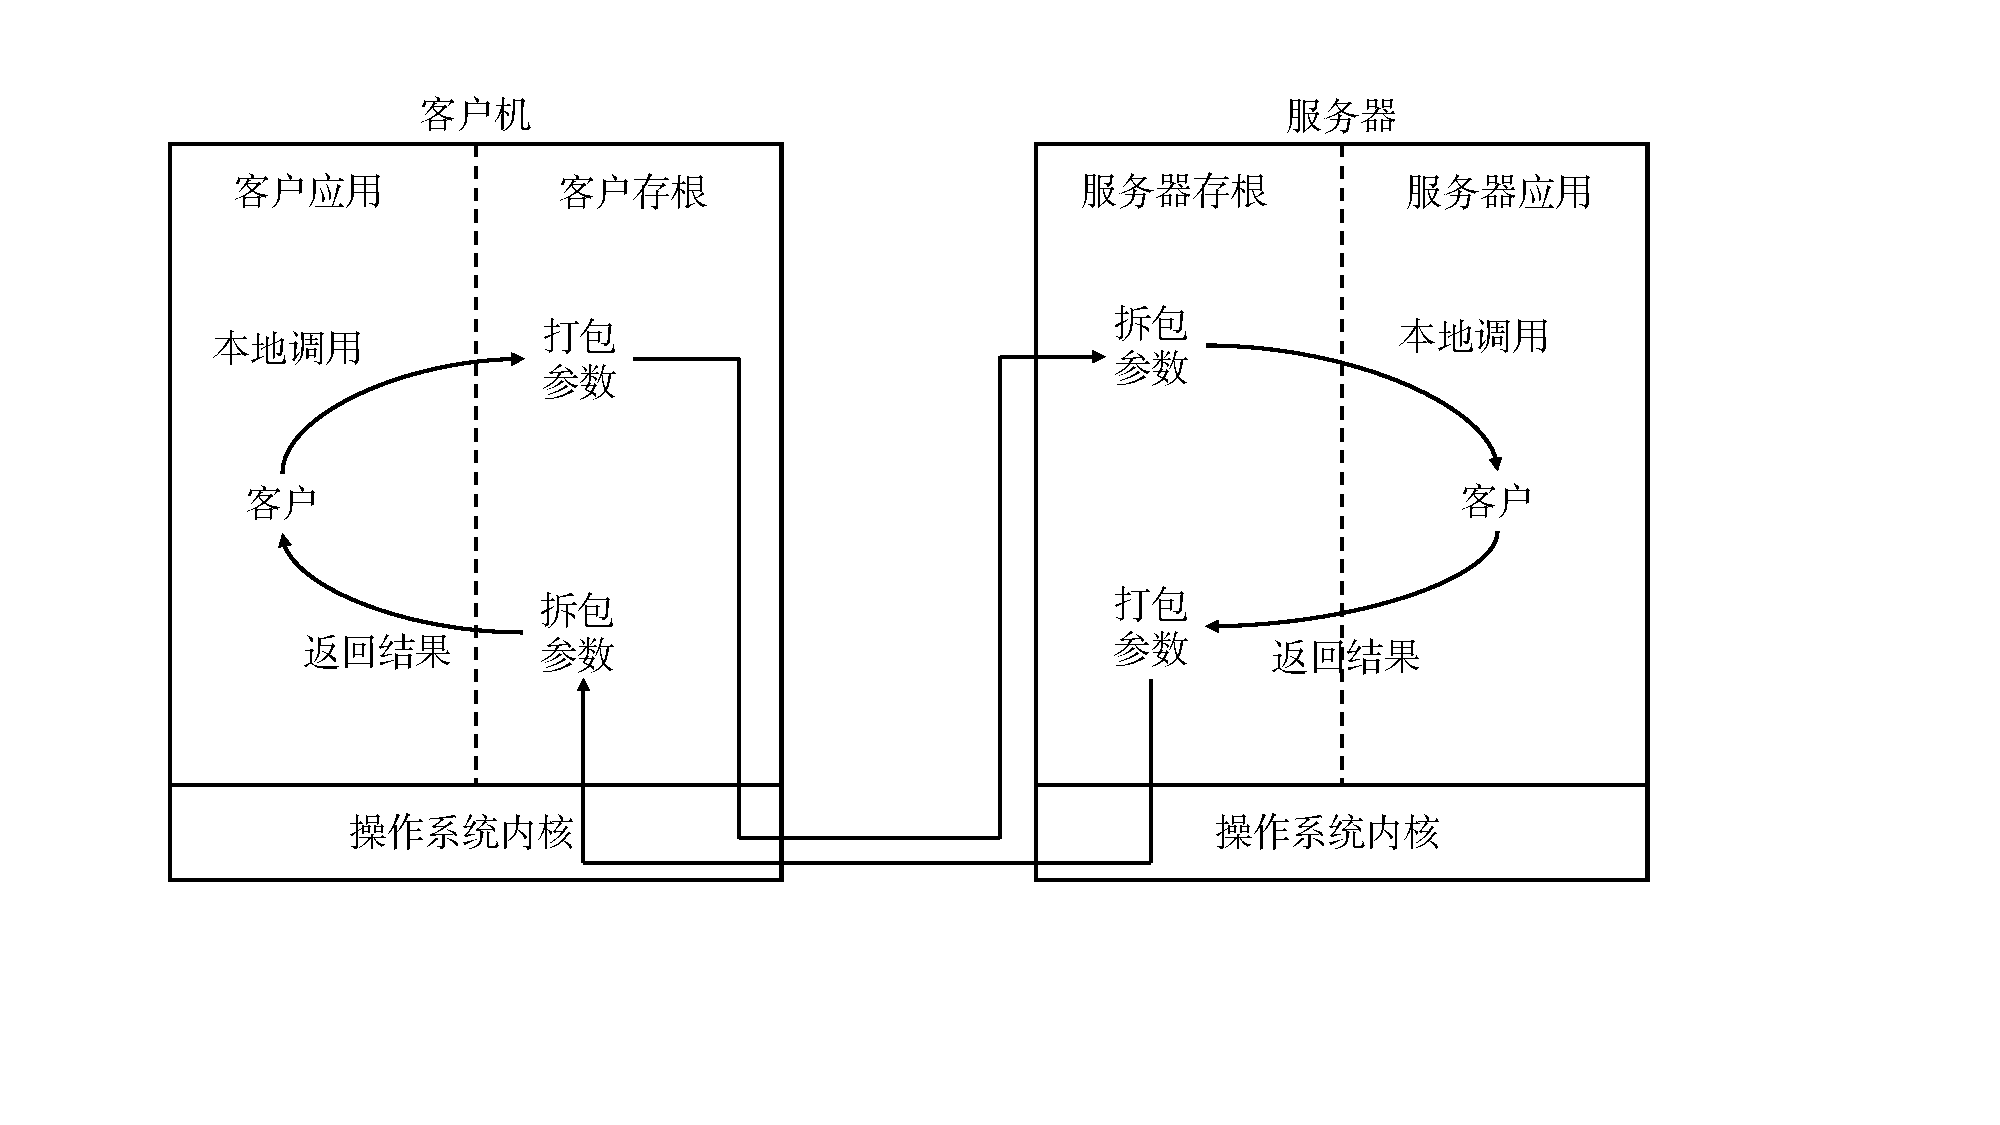
\includegraphics[width=0.75\textwidth]{img/远程过程调用机制.pdf}
	\end{figure}

	\section{死锁}
	\subsection{死锁的产生}

	\subsubsection{死锁的定义}
	在许多应用中,一个进程需要独占访问不止一个资源,当操作系统允许多个进程并发执行共享系统资源时,可能会出现所有进程被永久阻塞的现象,这时就产生了死锁

	一组进程处于死锁状态是指,如果在一个进程集合中,每个进程都在等待只能由该集合中的另一个进程才能引发的事件,则称一组进程或系统此时发生了死锁
	\begin{itemize}
		\item 例如,存在$n$个进程$P_1,P_2,\cdots,P_n$
		\item 进程$P_i(i=1,2,\cdots,n)$因为申请不到资源$R_j(j=1,\cdots,m)$而处于等待状态
		\item 而$R_j$又被$P_{i+1},(i=1,\cdots,n-1)$占有,$P_n$欲申请的资源被$P_1$占有
		\item 显然,此时这$n$个进程的等待状态永远不能结束,这$n$个进程处于死锁状态
	\end{itemize}

	\subsubsection{死锁的产生}
	死锁的产生不仅与系统拥有的资源数量有关,而且与资源分配策略,进程对资源的使用要求以及并发进程的推进顺序有关

	\paragraph{进程推进顺序不当产生死锁}~{}

	设系统有打印机、绘图仪各一台,被进程Q1和 Q2共享。两个进程并发执行,按下列次序请求和释放资源:
	\begin{figure}[H]
		\centering
		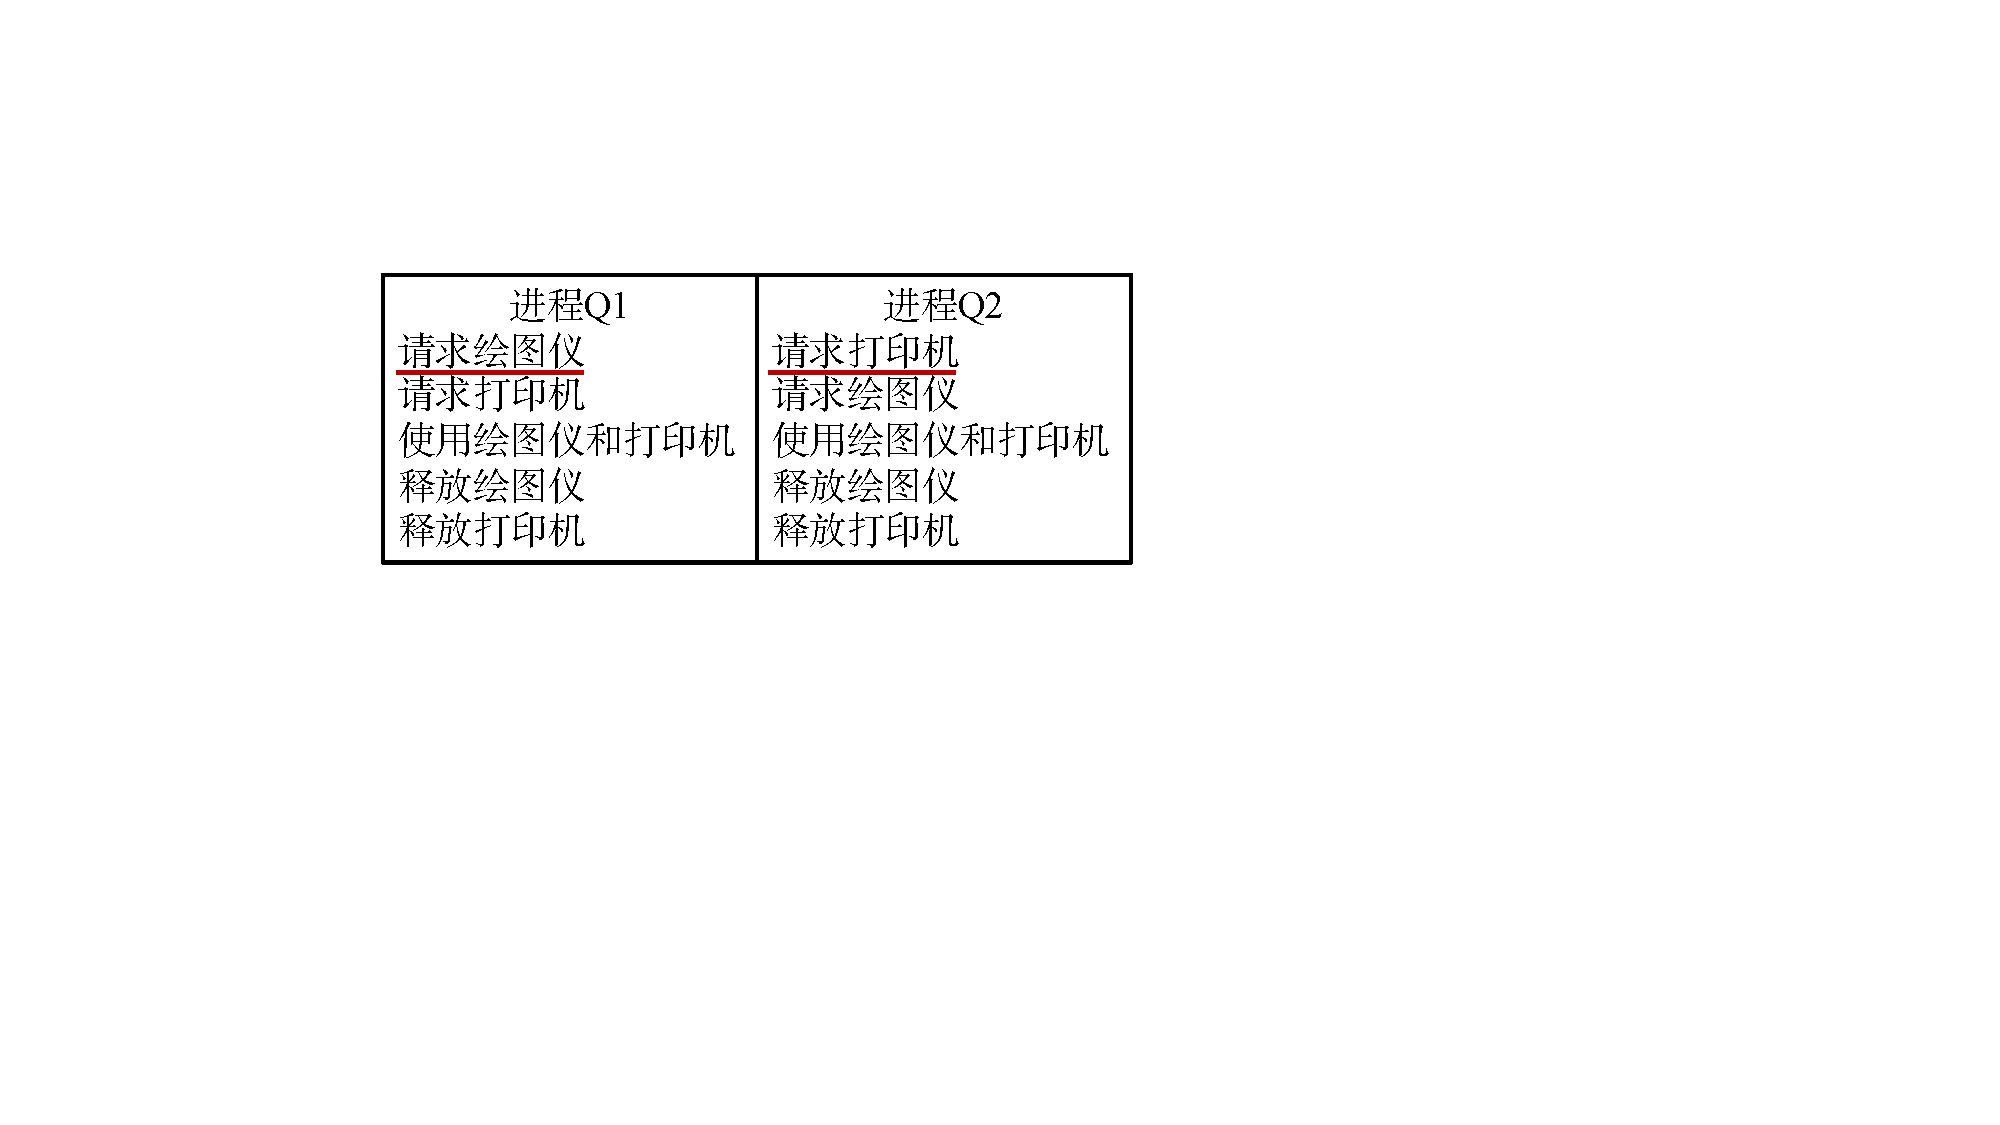
\includegraphics[width=0.45\textwidth]{img/进程推进顺序不当产生死锁.pdf}
	\end{figure}

	\paragraph{PV操作使用不当产生死锁}~{}


	\begin{figure}[H]
		\centering
		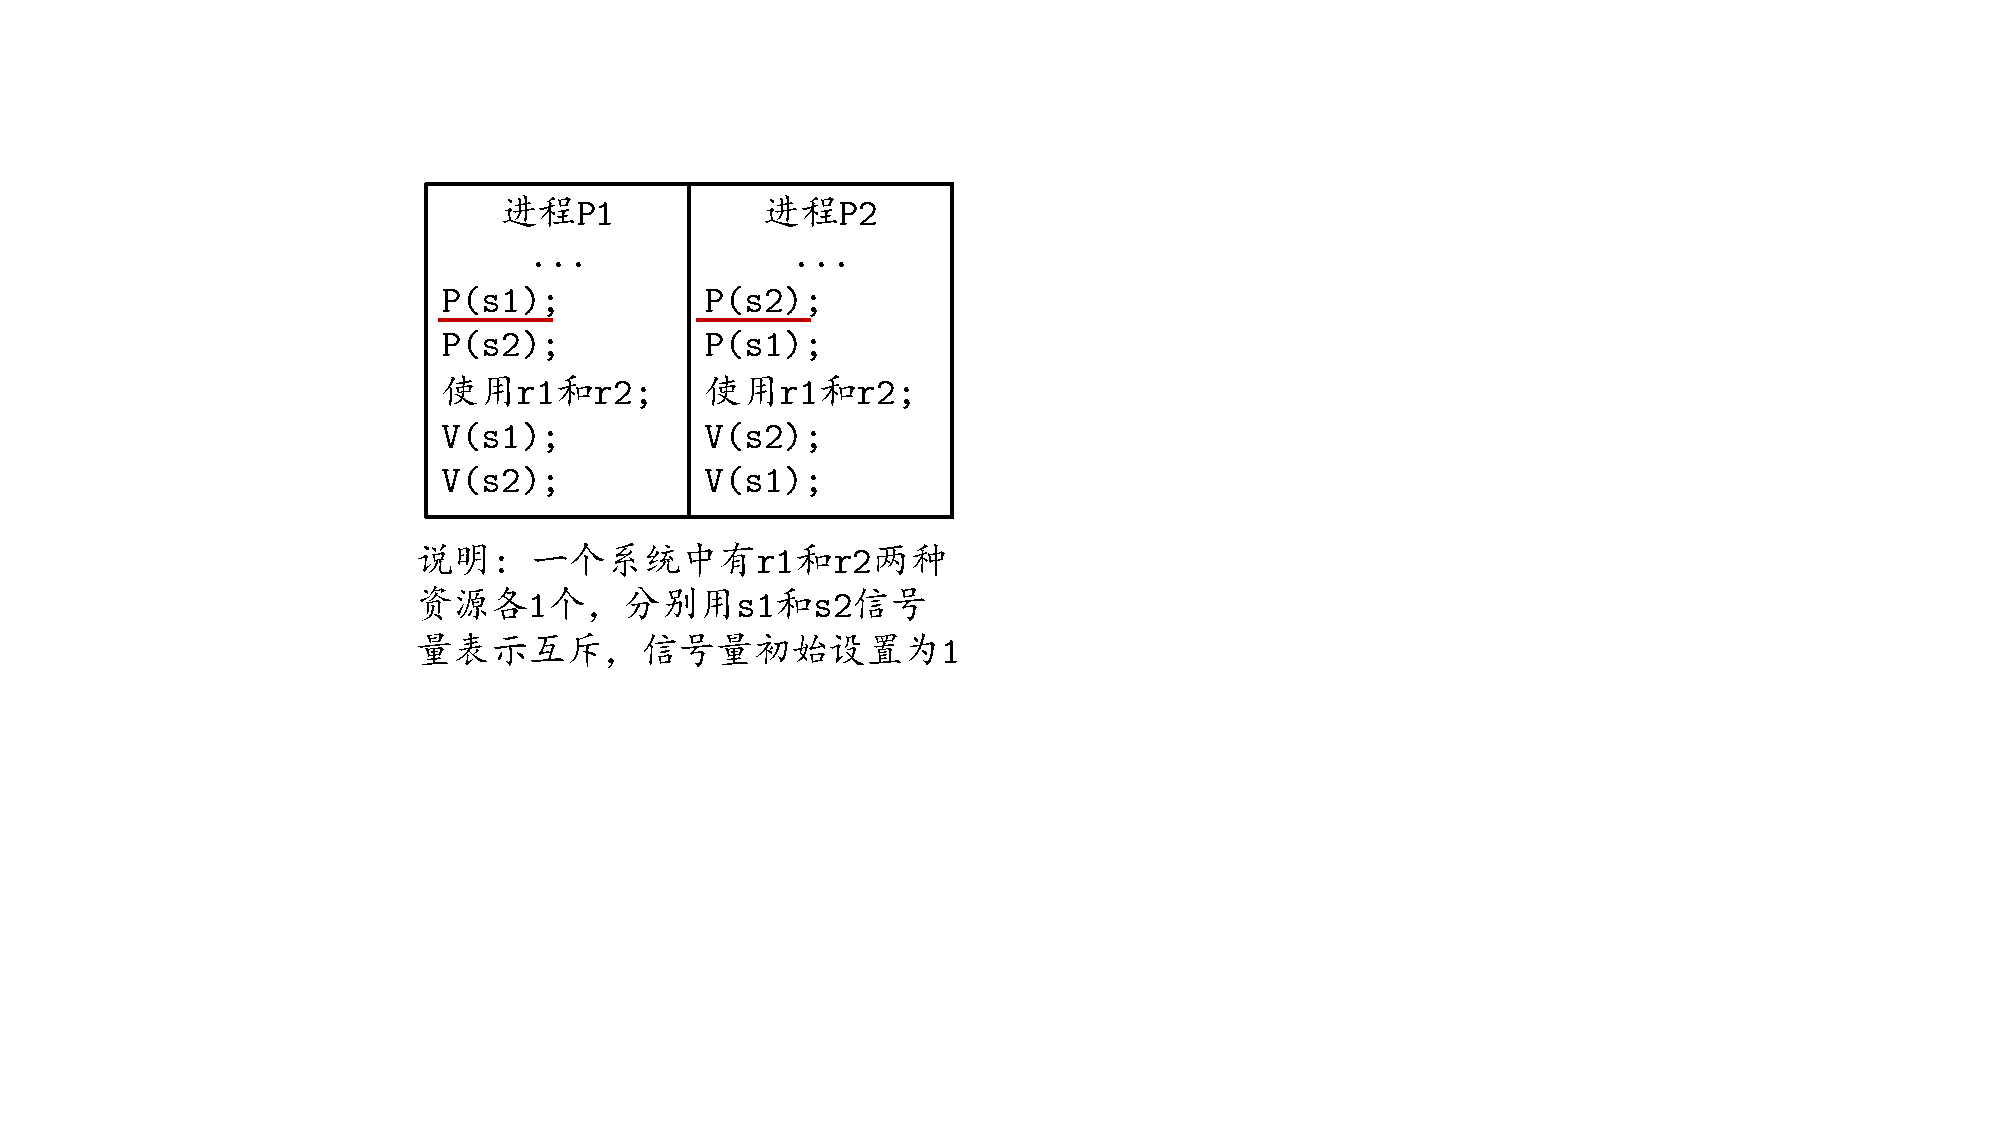
\includegraphics[width=0.3\textwidth]{img/PV操作使用不当产生死锁.pdf}
	\end{figure}

	\paragraph{资源分配不当引起死锁}~{}

	若系统中有$m$个资源被$n$个进程共享,每个进程都要求$K$个资源,而$m<nK$时,即资源数小于进程所要求的总数时,如果分配不当就可能引起死锁

	\paragraph{对临时性资源使用不加限制引起死锁}~{}

	进程通信使用的信件是一种临时性资源,如果对信件的发送和接收不加限制,可能引起死锁

	例如,进程$P_1$等待进程$P_3$的信件$S_3$来到后再向进程$P_2$发送信件$S_1$;$P_2$又要等待$P_1$的信件$S_1$来到后再向$P_3$发送信件$S_2$;而$P_3$也要等待$P_2$的信件$S_2$到来后才能发出信件$S_3$。这种情况下形成了循环等待,产生死锁

	\subsection{死锁的防止}

	\subsubsection{死锁产生的条件}
	系统形成死锁的四个必要条件:
	\begin{itemize}
		\item 互斥条件:系统中存在临界资源,进程应互斥地使用这些资源
		\item 占有和等待条件:进程请求资源得不到满足而等待时,不释放已占有的资源
		\item 不剥夺条件:已被占用的资源只能由属主释放,不允许被其它进程剥夺
		\item 循环等待条件:存在循环等待链,其中,每个进程都在链中等待下一个进程所持有的资源,造成这组进程永远等待
		\item 前三个条件是死锁存在的必要条件,但不是充分条件,第四个条件是前三个条件同时存在时所产生的结果
	\end{itemize}

	\subsubsection{死锁的防止}
	只要能破坏上述4个必要条件之一,就可防止死锁
	\begin{itemize}
		\item 破坏第一个条件,把独占型资源改造成共享性资源,使资源可同时访问而不是互斥使用。这是一个简单的办法,但对许多资源往往是不能做到的
		\item 采用剥夺式调度方法可以破坏第三个条件,但剥夺式调度方法目前只适用于对主存资源和处理器资源的分配,而不适用于所有资源
	\end{itemize}

	由于上述死锁的防止办法施加于资源的限制条件太严格,会造成资源利用率下降。下面介绍两种比较实用的死锁防止方法,它们能破坏占有和等待条件或循环等待条件

	\paragraph{静态分配策略}~{}

	静态分配是指一个进程必须在执行前就申请它需要的全部资源,并且直到它需要的资源都得到满足后才开始执行
	\begin{itemize}
		\item 破坏了占有和等待条件
		\item 该策略实现简单,被许多操作系统采用
		\item 但该策略严重地降低了资源利用率,因为在每个进程所占有的资源中,有些资源在进程较后的执行时间里才使用,甚至有些资源在例外的情况下才被使用
		\item 可能导致一个进程占有了一些在其执行周期中使用率很低的资源,而使其他想用这些资源的进程产生等待的结果
	\end{itemize}


	\paragraph{层次分配策略}~{}

	在层次分配策略下,资源被分成多个层次,一个进程得到某一层的一个资源后,它只能再申请较高一层的资源;当一个进程要释放某层的一个资源时,必须先释放所占用的较高层的资源;当另一个进程获得某一层的一个资源后,它想再申请该层中的另一个资源,必须先释放该层中的已占资源。
	\begin{itemize}
		\item 层次分配策略旨在阻止循环等待条件的出现
		\item 层次分配比静态分配在实现上要多花一点代价,但它提高了资源使用率
		\item 然而,如果一个进程使用资源的次序和系统内规定的各层资源的次序不同时,这种提高可能不明显
		\begin{itemize}
			\item 假如系统中的资源从高到低按序排列为:卡片输入机、行式打印机、卡片输出机、绘图仪和磁带机。若一个进程在执行中较早地使用绘图仪,而仅到快结束时才使用磁带机。但是,若系统规定磁带机所在层次低于绘图仪所在层次,则进程使用绘图仪前就必须先申请到磁带机,该磁带机就在很长一段时间里处于空闲状态直到进程执行到结束前才使用,这无疑是低效率的。
		\end{itemize}
	\end{itemize}


	\subsection{死锁的避免}
	当不能防止死锁的产生时,如果能掌握并发进程中与每个进程有关的资源申请情况,仍然可以避免死锁的发生

	银行家算法是由Dijkstra在1965年提出的一种资源分配算法:
	\begin{itemize}
		\item 检查申请者对各类资源的最大需求量,如果系统现存的各类资源可以满足它的最大需求量时,就满足当前的申请
		\item 换言之,仅仅在申请者可能无条件地归还它所申请的全部资源时,才分配资源给它
	\end{itemize}

	\subsubsection{银行家算法的数据结构}
	一个系统有$n$个进程和$m$种不同类型的资源,定义包含以下向量和矩阵的数据结构:
	\begin{itemize}
		\item 系统中每类资源总数向量:$\mathrm{Resource}=(R_1,R_2,...,R_m)$
		\item 系统中每类资源当前可用数向量:$\mathrm{Available}=(V_1,V_2,...,V_m)$
		\item 每个进程对各类资源的最大需求矩阵:$\mathrm{Claim}[i,j]$,对于$\mathrm{Claim}[i,j]=k$表示进程$P_i$需要$R_j$类资源的最大数目为$k$个
		\item 每个进程已占有各类资源数量矩阵:$\mathrm{Allocation}[i,j]$,对于$\mathrm{Allocation}[i,j] = k$表示进程$P_i$占有$R_j$类资源$k$个,初始值为0
		\item 每个进程尚需要各类资源数量矩阵$\mathrm{Need}[i,j]$,对于$\mathrm{Need}[i,j] = k$表示进程$P_i$还需要$R_j$类资源$k$个,$\mathrm{Need}[i,j] =\mathrm{Claim}[i,j] - \mathrm{Allocation}[i,j]$
		\item 每个进程从当前申请各类资源数量矩阵$\mathrm{Request}[i,j]$,对于$\mathrm{Request}[i,j] = k$,表示进程$P_i$当前申请$R_j$类资源$k$个
	\end{itemize}

	在银行家算法中下列关系式确保成立:
	\begin{itemize}
		\item 系统要启动一个新进程工作,对于资源$\mathrm{Resource}[i]$即$R_i$的需求满足不等式:
		$$R_i \geq \mathrm{Claim}[(n+1), i] + \sum\limits_{k=1}\limits^n \mathrm{Claim}[k, i]$$
		也就是应当满足当前系统中所有进程对资源$R_i$的最大需求数,加上启动的新进程的资源最大需求数,不超过系统拥有的最大资源数时才启动该进程(进程拒绝启动法)
		\item 所有资源要么被分配,要么尚可分配:
		$$R_i=V_i+\sum A_{ki},\quad  i=1,\cdots,m,\ k=1,\cdots,n$$
		\item 进程申请资源数不能超过系统拥有的资源总数:
		$$C_{ki} \leq R_i,\quad i=1,\cdots,m,\ k=1,\cdots,n$$
		\item 进程申请任何类资源数不能超过声明的最大资源需求数:
		$$A_{ki} \leq C_{ki},\quad i=1,\cdots,m,\ k=1,\cdots,n$$
	\end{itemize}
	

	\subsubsection{银行家算法的思想与实现}
	系统安全性:在时刻$T_0$系统是安全的,当且仅当存在一个进程序列$P_1,..,P_n$,对进程$P_k$满足公式:
	$$ \mathrm{Need}[k, i] \leq \mathrm{Available}[i](V_i) + \sum\limits_{j=1}\limits^{k-1}\mathrm{Allocation}[j, i]\quad i = 1,\cdots,m;\ k = 1,\cdots,n$$

	银行家算法的基本思想\footnote{安全序列并不是唯一的}
	\begin{enumerate}[label=\arabic*.]
		\item 系统中的所有进程进入进程集合
		\item 在安全状态下系统收到进程的资源请求后,先把资源试探性分配给它
		\item 系统用剩下的可用资源和进程集合中其他进程还要的资源数作比较,在进程集合中找到剩余资源能满足最大需求量的进程,从而,保证这个进程运行完毕并归还全部资源
		\item 把这个进程从集合中去掉,系统的剩余资源更多了,反复执行上述步骤(进程退出系统,资源回收)
		\item 最后,检查进程集合,若为空表明本次申请可行,系统处于安全状态,可实施本次分配;否则,有进程执行不完,系统处于不安全状态,本次资源分配暂不实施,让申请进程等待	
	\end{enumerate}

	银行家算法的程序及实现:
	\begin{enumerate}[label=\arabic*.]
		\item 如果$Request[i, *]\leq Need[i, *]$,转步骤2;否则,进程申请量超过最大需求量,出错处理
		\item 如果$Request[i, *]\leq Available[*]$,转步骤3;否则,申请量超过当前系统所拥有的可分配量,让进程$P_i$等待
		\item 系统对$P_i$进程请求资源执行试探性分配,执行
		$$\begin{aligned}
			Allocation[i,*] & = Allocation[i,*] + Request[i,*] \\
			Available[*] & = Available[*] - Request[i,*] \\
			Need[i,*] & = Need[i,*] - Request[i,*] 
		\end{aligned}$$
		\item 转向5去执行安全性测试算法,如果返回安全状态则承认试分配,否则抛弃试分配,进程$P_i$等待,并执行		
		$$\begin{aligned}
			Allocation[i,*] & = Allocation[i,*] - Request[i,*] \\
			Available[*] & = Available[*] + Request[i,*] \\
			Need[i,*] & = Need[i,*] + Request[i,*] 
		\end{aligned}$$
		\item 安全性测试算法
		\begin{enumerate}[label=(\arabic*)]
			\item 定义工作向量$Work[i]$、布尔型标志$possible$和进程集合$rest$
			\item 执行初始化操作:让全部进程进入$rest$集合,并让
			$$Work[*] = Available[*],\quad possible = true$$
			\item 保持$possible=true$,从进程集合$rest$中找出满足下列条件的进程$P_k$
			$$Need[k,*]\leq Work[*]$$
			\item 如果不存在,则转向(5);如果找到,则释放进程$P_k$所占用的资源,并执行以下操作:
			$$Work[*] = Work[*] + Allocation[k,*]$$
			把$P_k$从进程集合中去掉,即$rest = rest - \{P_k\}$,再转向(3)
			\item 置$possible = false$,停止执行本算法
			\item 最后查看进程集合$rest$,若为空则返回安全标记,否则返回不安全标记
		\end{enumerate}
	\end{enumerate}

	\begin{lstlisting}[language=C,keywordstyle=\color{black}]
typedef struct state { //全局数据结构
	int resource[m];
	int available[m];
	int claim[n][m];
	int allocation[n][m];
};

void resource_allocation( ) { //资源分配算法
   	if(allocation[i, *] + request[*] > claim[i, *])
    	{error}; //申请量超过最大需求值
	else {
    	if(request[*] > available[*])
    		{suspend process};
    	else{ //尝试分配,define newstate by:
        	allocation[i, *] = allocation[i, *] + request[*];
        	available[*] = available[*] - request[*];
      	}
   }
	if(safe(newstate))
		{carry out allocation};
	else{
		{restore original state};
		{suspend process};
   }
}

bool safe(state s) { //安全性测试算法
	int currentavail[m];
	set<process> rest;
	currentavail[*] = available[*];
	rest = {all process};
	possible = true;
	while(possible){ //rest中找一个Pk,满足以下条件
		claim[k, *] - allocation[k, *] <= currentavail[*];
		if(found){
			currentavail[*] = currentavail[*] + allocation[k, *];
			rest = rest – {Pk};
		}else{
			possible = false;
		}
	}
	return(rest = null);
}
	\end{lstlisting}

	\textbf{例:}如果系统中共有五个进程和$A$、$B$、$C$三类资源,$A$类资源共有10个,$B$类资源共有5个,$C$类资源共有7个,在时刻$T_0$,系统目前资源分配情况如下:

	\begin{table}[H]
	\centering
	\begin{tabular}{c|ccc|ccc|ccc|ccc}
	\hline
	\multirow{2}{*}{process} & \multicolumn{3}{c|}{Allocation} & \multicolumn{3}{c|}{Claim} & \multicolumn{3}{c|}{Available} & \multicolumn{3}{c}{Need} \\ \cline{2-13} 
							 & A         & B        & C        & A       & B       & C      & A        & B        & C        & A      & B      & C      \\ \hline
	$P_0$                    & 0         & 1        & 0        & 7       & 5       & 3      & 3        & 3        & 2        & 7      & 4      & 3      \\ \hline
	$P_1$                    & 2         & 0        & 0        & 3       & 2       & 2      &          &          &          & 1      & 2      & 2      \\ \hline
	$P_2$                    & 3         & 0        & 2        & 9       & 0       & 2      &          &          &          & 6      & 0      & 0      \\ \hline
	$P_3$                    & 2         & 1        & 1        & 2       & 2       & 2      &          &          &          & 0      & 1      & 1      \\ \hline
	$P_4$                    & 0         & 0        & 2        & 4       & 3       & 3      &          &          &          & 4      & 3      & 1      \\ \hline
	\end{tabular}
	\end{table}

	可以断言目前系统处于安全状态,因为序列$\{P_1,P_3,P_4,P_2,P_0\}$能满足安全性条件
	\begin{table}[H]
	\centering
	\begin{tabular}{c|ccc|ccc|ccc|ccc|c}
	\hline
	\multirow{2}{*}{process} & \multicolumn{3}{c|}{Work} & \multicolumn{3}{c|}{Need} & \multicolumn{3}{c|}{Allocation} & \multicolumn{3}{c|}{Work+Allocation} & \multirow{2}{*}{possible} \\ \cline{2-13}
							 & A       & B      & C      & A       & B      & C      & A         & B        & C        & A           & B          & C         &                           \\ \hline
	$P_1$                    & 3       & 3      & 2      & 1       & 2      & 2      & 2         & 0        & 0        & 5           & 3          & 2         & true                      \\ \hline
	$P_3$                    & 5       & 3      & 2      & 0       & 1      & 1      & 2         & 1        & 1        & 7           & 4          & 3         & true                      \\ \hline
	$P_4$                    & 7       & 4      & 3      & 4       & 3      & 1      & 0         & 0        & 2        & 7           & 4          & 5         & true                      \\ \hline
	$P_2$                    & 7       & 4      & 5      & 6       & 0      & 0      & 3         & 0        & 2        & 10          & 4          & 7         & true                      \\ \hline
	$P_0$                    & 10      & 4      & 7      & 7       & 4      & 3      & 0         & 1        & 0        & 10          & 5          & 7         & true                      \\ \hline
	\end{tabular}
	\end{table}

	假设$P_1$又请求1个$A$类资源和2个$C$类资源,得到新的状态如下图所示:
	$$Request1(1,0,2)\leq Need(1,2,2) \quad Request1(1, 0, 2) \leq Available(3, 3, 2)$$
	\begin{table}[H]
	\centering
	\begin{tabular}{c|ccc|ccc|ccc}
	\hline
	\multirow{2}{*}{process} & \multicolumn{3}{c|}{Allocation} & \multicolumn{3}{c|}{Need} & \multicolumn{3}{c}{Available} \\ \cline{2-10} 
							 & A         & B        & C        & A       & B      & C      & A        & B        & C       \\ \hline
	$P_0$                    & 0         & 1        & 0        & 7       & 4      & 3      & 2        & 3        & 0       \\ \hline
	$P_1$                    & 3         & 0        & 2        & 0       & 2      & 0      &          &          &         \\ \hline
	$P_2$                    & 3         & 0        & 2        & 6       & 0      & 0      &          &          &         \\ \hline
	$P_3$                    & 2         & 1        & 1        & 0       & 1      & 1      &          &          &         \\ \hline
	$P_4$                    & 0         & 0        & 2        & 4       & 3      & 1      &          &          &         \\ \hline
	\end{tabular}
	\end{table}


	判定新状态是否安全:执行安全性测试算法,找到一个进程序列$\{P_1,P_3,P_4,P_0,P_2\}$能满足安全性条件,所以可正式把资源分配给进程$P_1$
	\begin{table}[H]
	\centering
	\begin{tabular}{c|ccc|ccc|ccc|ccc|c}
	\hline
	\multirow{2}{*}{process} & \multicolumn{3}{c|}{Work} & \multicolumn{3}{c|}{Need} & \multicolumn{3}{c|}{Allocation} & \multicolumn{3}{c|}{Work+Allocation} & \multirow{2}{*}{possible} \\ \cline{2-13}
							 & A       & B      & C      & A       & B      & C      & A         & B        & C        & A           & B          & C         &                           \\ \hline
	$P_1$                    & 2       & 3      & 0      & 0       & 2      & 0      & 3         & 0        & 2        & 5           & 3          & 2         & true                      \\ \hline
	$P_3$                    & 5       & 3      & 2      & 0       & 1      & 1      & 2         & 1        & 1        & 7           & 4          & 3         & true                      \\ \hline
	$P_4$                    & 7       & 4      & 3      & 4       & 3      & 1      & 0         & 0        & 2        & 7           & 4          & 5         & true                      \\ \hline
	$P_0$                    & 7       & 4      & 5      & 7       & 4      & 3      & 0         & 1        & 0        & 7           & 5          & 5         & true                      \\ \hline
	$P_2$                    & 7       & 5      & 5      & 6       & 0      & 0      & 3         & 0        & 2        & 10          & 5          & 7         & true                      \\ \hline
	\end{tabular}
	\end{table}

	假设$P_4$发起资源请求,按照银行家算法检查,资源不足不予以分配
	$$Request4(3, 3, 0) \leq Need(4, 3, 1) \quad Request4(3, 3, 0) > Available(2, 3, 0)$$


	假设$P_0$发起资源请求,按照银行家算法检查,得到中间结果如下
	$$Request0(0, 2, 0) \leq Need(7, 3, 1) \quad Request0(0, 2, 0) \leq Available(2, 3, 0)$$
	\begin{table}[H]
	\centering
	\begin{tabular}{c|ccc|ccc|ccc}
	\hline
	\multirow{2}{*}{process} & \multicolumn{3}{c|}{Allocation} & \multicolumn{3}{c|}{Need} & \multicolumn{3}{c}{Available} \\ \cline{2-10} 
							 & A         & B        & C        & A       & B      & C      & A        & B        & C       \\ \hline
	$P_0$                    & 0         & 3        & 0        & 7       & 2      & 3      & 2        & 1        & 0       \\ \hline
	$P_1$                    & 3         & 0        & 2        & 0       & 2      & 0      &          &          &         \\ \hline
	$P_2$                    & 3         & 0        & 2        & 6       & 0      & 0      &          &          &         \\ \hline
	$P_3$                    & 2         & 1        & 1        & 0       & 1      & 1      &          &          &         \\ \hline
	$P_4$                    & 0         & 0        & 2        & 4       & 3      & 1      &          &          &         \\ \hline
	\end{tabular}
	\end{table}
	但可以看出系统已处于不安全状态了。

	\subsection{死锁的检测}
	解决死锁问题的一条途径是死锁的检测和解除
	\begin{itemize}
		\item 这种方法对资源的分配不加任何限制,也不采取死锁的避免措施
		\item 系统定时地运行一个死锁的检测程序,判断系统内是否已出现死锁,如果检测到系统已发生了死锁,再采取措施解除
	\end{itemize}

	死锁的检测可设置两张表格来记录进程使用资源的情况,其中等待资源表记录每个被阻塞进程等待的资源,占用资源表记录每个进程占有的资源
	\begin{itemize}
		\item 任一进程申请资源时,先检查该资源是否为其他进程所占用
		\item 若资源空闲,则将该资源分配给申请者且登入占用资源表
		\item 若该资源被其他进程占用,则登入进程等待资源表
	\end{itemize}
	\begin{center}
		\begin{minipage}[c]{0.2\textwidth}
			\centering
				\begin{tabular}{|c|c|}
				\hline
				资源       & 占用进程     \\ \hline
				$r_1$    & $P_1$    \\ \hline
				$r_2$    & $P_2$    \\ \hline
				$r_3$    & $P_3$    \\ \hline
				$r_4$    & $P_4$    \\ \hline
				$r_5$    & $P_5$    \\ \hline
				$\cdots$ & $\cdots$ \\ \hline
				\end{tabular}
		\end{minipage}
		\hspace{.15in}
		\begin{minipage}[c]{0.2\textwidth}
			\centering
				\begin{tabular}{|c|c|}
				\hline
				进程       & 等待资源     \\ \hline
				$P_1$    & $r_1$    \\ \hline
				$P_2$    & $r_2$    \\ \hline
				$P_3$    & $r_3$    \\ \hline
				$\cdots$ & $\cdots$ \\ \hline
				\end{tabular}
		\end{minipage}
	\end{center}
	死锁检测程序定时检测这两张表,如果有进程$P_i$等待资源$r_k$,且$r_k$被进程$P_j$占用,则说明$P_i$和$P_j$具有等待占用关系,记为$W(P_i,P_j)$。死锁检测程序反复检测这两张表列出所有的等待占用关系,当出现$W(P_i,P_j),W(P_j,P_k),\cdots,W(P_1,P_m),W(P_m,P_i)$时,系统中就存在一组循环等待资源的进程$P_i,P_j,P_k,$\\$\cdots,P_1,P_m$,也就表明系统出现了死锁。

	\subsubsection{利用等待资源表和占用资源表进行死锁检测}
	将等待资源表和占用资源表中记录的进程使用和资源等待的情况用一个矩阵$\boldsymbol{A}$来表示
	$$
	\boldsymbol{A}[b_{ij}]=\left(
		\begin{array}{cccc}
			b_{11} & b_{12} & \cdots & b_{1n} \\
			b_{21} & b_{22} & \cdots & b_{2n} \\
			\vdots & \vdots &        & \vdots \\
			b_{n1} & b_{n2} & \cdots & b_{nn} \\
		\end{array}
	\right)
	$$
	当$P_i$等待被$P_j$占用的资源时,$b_{ij}$的值记为1;当$P_i$和$P_j$不存在资源等待占用关系时,$b_{ij}$的值记为0

	死锁检测程序可用Warshall的传递闭包算法来检测系统是否有死锁发生
	\begin{itemize}
		\item Warshall的传递闭包算法基于状态矩阵$\boldsymbol{A}$构成传递闭包$\boldsymbol{A} *[b_{ij}]$
		\item $\boldsymbol{A} *[b_{ij}]$中的每个$b_{ij}$是对$\boldsymbol{A}[b_{ij}]$执行如下算法得到的
		\begin{lstlisting}[language=C, keywordstyle=\color{black}]
for(int k = 1; k <= n; k++)
	for(int i = 1; i <= n; i++)
    	for(int j = 1; j <= n; j++)
			bij = bij OR (bik AND bkj)
		\end{lstlisting}
		\item 其中,$b_{ij}$表示进程$P_i$与进程$P_j$存在直接等待关系
		\item 当进程$P_i$等待进程$P_k$所占用的资源且进程$P_k$等待进程$P_j$所占用的资源时,$b_{ik} \land b_{kj} $取值为1。也就是说,进程$P_i$进程$P_j$之间具有间接等待关系
		\item Warshall传递闭包算法循环检测了矩阵$\boldsymbol{A}$中的各个元素,将直接等待资源关系和间接等待资源关系都在传递闭包$\boldsymbol{A}*$中表示出来
		\item 显然,当$\boldsymbol{A}*$中存在一个$b_{ii} = 1(i=1,2,\cdots,n)$时,就说明存在一组进程处于循环等待资源状态,即系统出现了死锁
	\end{itemize}


	\subsubsection{进程-资源分配图与死锁的检测}
	进程-资源分配图
	\begin{itemize}
		\item 约定$P_i \to R_j$为请求边,表示进程$P_i$申请资源类$R_j$中的一个资源得不到满足而处于等待$R_j$类资源的状态,该有向边从进程开始指到方框的边缘,表示进程$P_i$申请$R_j$类中的一个资源。
		\item 约定$R_j \to P_i$为分配边,表示$R_j$类中的一个资源已被进程$P_i$占用,由于已把一个具体的资源分给了进程$P_i$,故该有向边从方框内的某个黑圆点出发指向进程。
	\end{itemize}

	\begin{figure}[H]
		\centering
		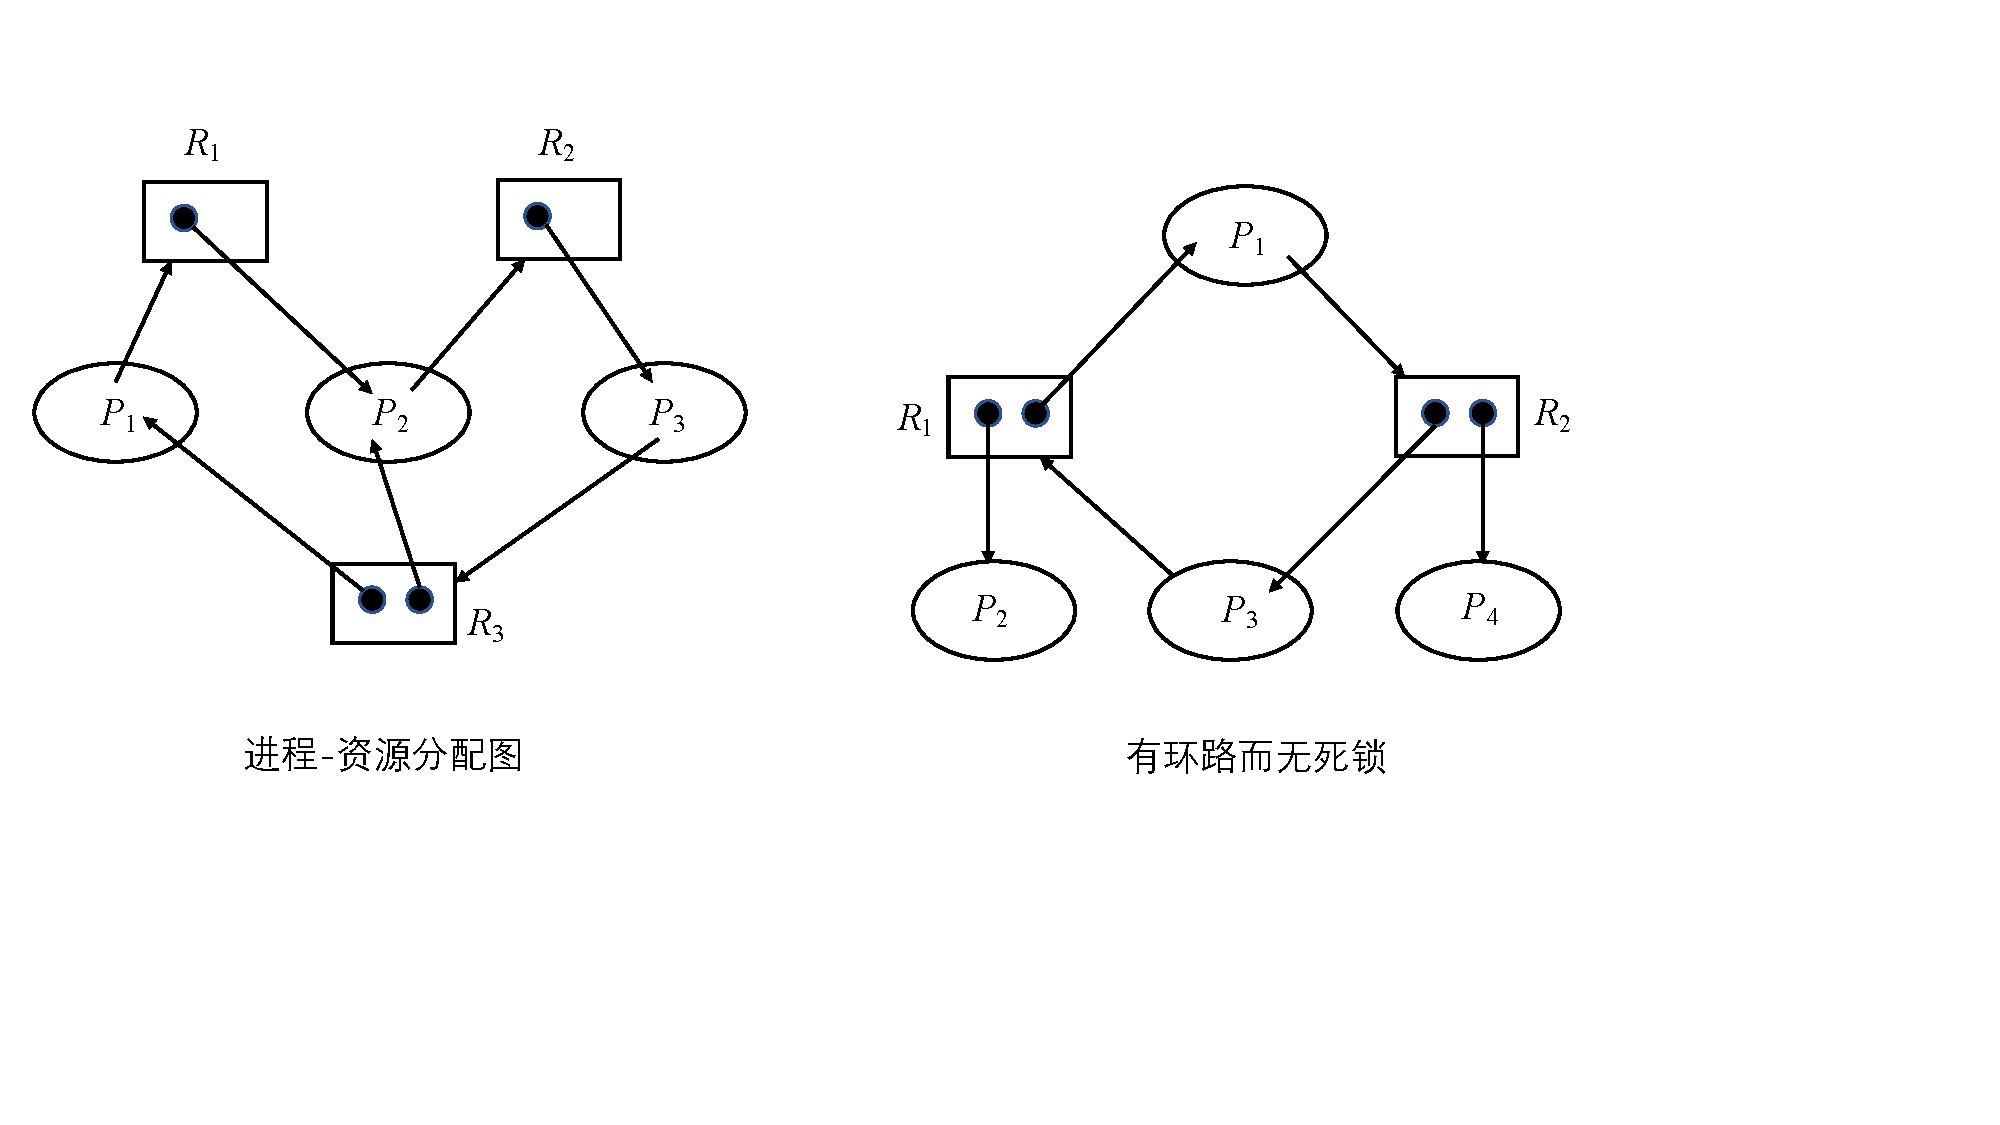
\includegraphics[width=0.7\textwidth]{img/进程-资源分配图.pdf}
	\end{figure}

	利用资源分配图检测系统是否处于死锁状态
	\begin{itemize}
		\item 如果进程-资源分配图中无环路,则此时系统没有发生死锁
		\item 如果进程-资源分配图中有环路,且每个资源类中仅有一个资源,则系统中发生了死锁,此时,环路是系统发生死锁的充要条件,环路中的进程便为死锁进程
		\item 如果进程-资源分配图中有环路,且涉及的资源类中有多个资源,则环路的存在只是产生死锁的必要条件而不是充分条件
		\begin{itemize}
			\item 如果能在进程-资源分配图中消去此进程的所有请求边和分配边,这样的进程称为孤立结点。经一系列简化,使所有进程成为孤立结点,则该图是可完全简化的;否则则称该图是不可完全简化的。
			\item 系统为死锁状态的充分条件是:当且仅当该状态的进程-资源分配图是不可完全简化的,该充分条件称为死锁定理。
		\end{itemize}
	\end{itemize}

	死锁检测算法相应的数据结构:
	\begin{enumerate}[label=\arabic*.]
		\item $Available[m]$是长度为$m$的向量,说明每类资源中可供分配的资源数目
		\item $Allocation[n,m]$是$n\times m$矩阵,说明已分配给每个进程的每类资源数目
		\item $Request[n,m]$是$n\times m$矩阵,说明当前每个进程对每类资源的申请数目
		\item $Work[m]$是长度为$m$的工作向量
		\item $finish[n]$是长度为$n$的布尔型工作向量
	\end{enumerate}
	令$k=1,2,\cdots,n$,死锁检测算法的步骤如下:
	\begin{enumerate}[label=\arabic*.]
		\item $Work[*] = Available[*]$
		\item 如果$Allocation[k,*] \neq 0$,令$finish[k]=false$;否则$finish[k]=true$
		\item 寻找一个$k$,应满足条件
		$$(finish[k]==false)\&\&(Request[k,*]\leq Work[*])$$
		若找不到这样的$k$,则转向5
		\item 修改$Work[*] = Work[*]+Allocation[k,*],finish[k]=true$,然后转向3
		\item 如果存在$k(1\leq k\leq n),finish[k]=false$,则系统处于死锁状态,并且$finish[k]=false$的$P_k$是处于死锁的进程
	\end{enumerate}
	

	\subsubsection{死锁的解除}
	\begin{itemize}
		\item 结束所有进程的执行,重新启动操作系统。该方法简单,但以前的工作全部作废,损失很大。
		\item 撤销陷于死锁的所有进程,解除死锁,重新启动执行。这种方法的代价也相当大。
		\item 逐个撤销陷于死锁的进程,回收其资源重新分派,直至死锁解除。
		\item 剥夺陷于死锁的进程占用的资源,但并不撤销它,直至死锁解除。可仿照撤销陷于死锁进程的条件来选择剥夺资源的进程。
		\item 根据系统保存的检查点,让所有进程回退,直到足以解除死锁,这种措施要求系统建立保存检查点、回退及重启机制。
		\item 当检测到死锁时,如果存在某些未卷入死锁的进程,而随着这些进程执行到结束,有可能释放足够的资 源来解除死锁。
	\end{itemize}




	

\end{document}


